\documentclass[twoside]{book}

% Packages required by doxygen
\usepackage{fixltx2e}
\usepackage{calc}
\usepackage{doxygen}
\usepackage[export]{adjustbox} % also loads graphicx
\usepackage{graphicx}
\usepackage[utf8]{inputenc}
\usepackage{makeidx}
\usepackage{multicol}
\usepackage{multirow}
\PassOptionsToPackage{warn}{textcomp}
\usepackage{textcomp}
\usepackage[nointegrals]{wasysym}
\usepackage[table]{xcolor}

% Font selection
\usepackage[T1]{fontenc}
\usepackage[scaled=.90]{helvet}
\usepackage{courier}
\usepackage{amssymb}
\usepackage{sectsty}
\renewcommand{\familydefault}{\sfdefault}
\allsectionsfont{%
  \fontseries{bc}\selectfont%
  \color{darkgray}%
}
\renewcommand{\DoxyLabelFont}{%
  \fontseries{bc}\selectfont%
  \color{darkgray}%
}
\newcommand{\+}{\discretionary{\mbox{\scriptsize$\hookleftarrow$}}{}{}}

% Page & text layout
\usepackage{geometry}
\geometry{%
  a4paper,%
  top=2.5cm,%
  bottom=2.5cm,%
  left=2.5cm,%
  right=2.5cm%
}
\tolerance=750
\hfuzz=15pt
\hbadness=750
\setlength{\emergencystretch}{15pt}
\setlength{\parindent}{0cm}
\setlength{\parskip}{3ex plus 2ex minus 2ex}
\makeatletter
\renewcommand{\paragraph}{%
  \@startsection{paragraph}{4}{0ex}{-1.0ex}{1.0ex}{%
    \normalfont\normalsize\bfseries\SS@parafont%
  }%
}
\renewcommand{\subparagraph}{%
  \@startsection{subparagraph}{5}{0ex}{-1.0ex}{1.0ex}{%
    \normalfont\normalsize\bfseries\SS@subparafont%
  }%
}
\makeatother

% Headers & footers
\usepackage{fancyhdr}
\pagestyle{fancyplain}
\fancyhead[LE]{\fancyplain{}{\bfseries\thepage}}
\fancyhead[CE]{\fancyplain{}{}}
\fancyhead[RE]{\fancyplain{}{\bfseries\leftmark}}
\fancyhead[LO]{\fancyplain{}{\bfseries\rightmark}}
\fancyhead[CO]{\fancyplain{}{}}
\fancyhead[RO]{\fancyplain{}{\bfseries\thepage}}
\fancyfoot[LE]{\fancyplain{}{}}
\fancyfoot[CE]{\fancyplain{}{}}
\fancyfoot[RE]{\fancyplain{}{\bfseries\scriptsize Generated by Doxygen }}
\fancyfoot[LO]{\fancyplain{}{\bfseries\scriptsize Generated by Doxygen }}
\fancyfoot[CO]{\fancyplain{}{}}
\fancyfoot[RO]{\fancyplain{}{}}
\renewcommand{\footrulewidth}{0.4pt}
\renewcommand{\chaptermark}[1]{%
  \markboth{#1}{}%
}
\renewcommand{\sectionmark}[1]{%
  \markright{\thesection\ #1}%
}

% Indices & bibliography
\usepackage{natbib}
\usepackage[titles]{tocloft}
\setcounter{tocdepth}{3}
\setcounter{secnumdepth}{5}
\makeindex

% Hyperlinks (required, but should be loaded last)
\usepackage{ifpdf}
\ifpdf
  \usepackage[pdftex,pagebackref=true]{hyperref}
\else
  \usepackage[ps2pdf,pagebackref=true]{hyperref}
\fi
\hypersetup{%
  colorlinks=true,%
  linkcolor=blue,%
  citecolor=blue,%
  unicode%
}

% Custom commands
\newcommand{\clearemptydoublepage}{%
  \newpage{\pagestyle{empty}\cleardoublepage}%
}

\usepackage{caption}
\captionsetup{labelsep=space,justification=centering,font={bf},singlelinecheck=off,skip=4pt,position=top}

%===== C O N T E N T S =====

\begin{document}

% Titlepage & ToC
\hypersetup{pageanchor=false,
             bookmarksnumbered=true,
             pdfencoding=unicode
            }
\pagenumbering{alph}
\begin{titlepage}
\vspace*{7cm}
\begin{center}%
{\Large tictactoe\+\_\+mcts \\[1ex]\large 1.\+0 }\\
\vspace*{1cm}
{\large Generated by Doxygen 1.8.13}\\
\end{center}
\end{titlepage}
\clearemptydoublepage
\pagenumbering{roman}
\tableofcontents
\clearemptydoublepage
\pagenumbering{arabic}
\hypersetup{pageanchor=true}

%--- Begin generated contents ---
\chapter{Namespace Index}
\section{Namespace List}
Here is a list of all namespaces with brief descriptions\+:\begin{DoxyCompactList}
\item\contentsline{section}{\hyperlink{namespacedbg}{dbg} }{\pageref{namespacedbg}}{}
\item\contentsline{section}{\hyperlink{namespacedbg_1_1detail}{dbg\+::detail} }{\pageref{namespacedbg_1_1detail}}{}
\item\contentsline{section}{\hyperlink{namespacedbg_1_1detail__detector}{dbg\+::detail\+\_\+detector} }{\pageref{namespacedbg_1_1detail__detector}}{}
\item\contentsline{section}{\hyperlink{namespacedbg_1_1pretty__function}{dbg\+::pretty\+\_\+function} }{\pageref{namespacedbg_1_1pretty__function}}{}
\item\contentsline{section}{\hyperlink{namespacegame}{game} }{\pageref{namespacegame}}{}
\item\contentsline{section}{\hyperlink{namespacegame_1_1penguin}{game\+::penguin} }{\pageref{namespacegame_1_1penguin}}{}
\item\contentsline{section}{\hyperlink{namespacegame_1_1tic__tac__toe}{game\+::tic\+\_\+tac\+\_\+toe} }{\pageref{namespacegame_1_1tic__tac__toe}}{}
\item\contentsline{section}{\hyperlink{namespacemcts}{mcts} }{\pageref{namespacemcts}}{}
\end{DoxyCompactList}

\chapter{Hierarchical Index}
\section{Class Hierarchy}
This inheritance list is sorted roughly, but not completely, alphabetically\+:\begin{DoxyCompactList}
\item \contentsline{section}{game\+:\+:Abstract\+Board$<$ CellT, PlayerT, PawnT $>$}{\pageref{classgame_1_1_abstract_board}}{}
\item \contentsline{section}{game\+:\+:Abstract\+Board$<$ Board\+Cell, Human\+Player, Penguin\+Pawn $>$}{\pageref{classgame_1_1_abstract_board}}{}
\begin{DoxyCompactList}
\item \contentsline{section}{game\+:\+:penguin\+:\+:Board}{\pageref{classgame_1_1penguin_1_1_board}}{}
\end{DoxyCompactList}
\item \contentsline{section}{game\+:\+:Abstract\+Board$<$ Board\+Cell, Player, Player $>$}{\pageref{classgame_1_1_abstract_board}}{}
\begin{DoxyCompactList}
\item \contentsline{section}{game\+:\+:tic\+\_\+tac\+\_\+toe\+:\+:Board}{\pageref{classgame_1_1tic__tac__toe_1_1_board}}{}
\end{DoxyCompactList}
\item \contentsline{section}{game\+:\+:Abstract\+Board\+Cell}{\pageref{classgame_1_1_abstract_board_cell}}{}
\begin{DoxyCompactList}
\item \contentsline{section}{game\+:\+:penguin\+:\+:Board\+Cell}{\pageref{classgame_1_1penguin_1_1_board_cell}}{}
\item \contentsline{section}{game\+:\+:tic\+\_\+tac\+\_\+toe\+:\+:Board\+Cell}{\pageref{classgame_1_1tic__tac__toe_1_1_board_cell}}{}
\end{DoxyCompactList}
\item \contentsline{section}{game\+:\+:Abstract\+Game$<$ CellT, PlayerT, PawnT $>$}{\pageref{classgame_1_1_abstract_game}}{}
\item \contentsline{section}{game\+:\+:Abstract\+Game$<$ Board\+Cell, Human\+Player, Penguin\+Pawn $>$}{\pageref{classgame_1_1_abstract_game}}{}
\begin{DoxyCompactList}
\item \contentsline{section}{game\+:\+:penguin\+:\+:Penguin\+Game}{\pageref{classgame_1_1penguin_1_1_penguin_game}}{}
\end{DoxyCompactList}
\item \contentsline{section}{game\+:\+:Abstract\+Game$<$ Board\+Cell, Player, Player $>$}{\pageref{classgame_1_1_abstract_game}}{}
\begin{DoxyCompactList}
\item \contentsline{section}{game\+:\+:tic\+\_\+tac\+\_\+toe\+:\+:Tic\+Tac\+Toe}{\pageref{classgame_1_1tic__tac__toe_1_1_tic_tac_toe}}{}
\begin{DoxyCompactList}
\item \contentsline{section}{game\+:\+:tic\+\_\+tac\+\_\+toe\+:\+:Console\+Game}{\pageref{classgame_1_1tic__tac__toe_1_1_console_game}}{}
\end{DoxyCompactList}
\end{DoxyCompactList}
\item \contentsline{section}{game\+:\+:Abstract\+Interface}{\pageref{classgame_1_1_abstract_interface}}{}
\begin{DoxyCompactList}
\item \contentsline{section}{game\+:\+:penguin\+:\+:Console\+Game}{\pageref{classgame_1_1penguin_1_1_console_game}}{}
\item \contentsline{section}{game\+:\+:tic\+\_\+tac\+\_\+toe\+:\+:Console\+Game}{\pageref{classgame_1_1tic__tac__toe_1_1_console_game}}{}
\end{DoxyCompactList}
\item \contentsline{section}{game\+:\+:Abstract\+Pawn$<$ PlayerT, CellT $>$}{\pageref{classgame_1_1_abstract_pawn}}{}
\item \contentsline{section}{game\+:\+:Abstract\+Pawn$<$ Human\+Player, Board\+Cell $>$}{\pageref{classgame_1_1_abstract_pawn}}{}
\begin{DoxyCompactList}
\item \contentsline{section}{game\+:\+:penguin\+:\+:Penguin\+Pawn}{\pageref{classgame_1_1penguin_1_1_penguin_pawn}}{}
\end{DoxyCompactList}
\item \contentsline{section}{game\+:\+:Abstract\+Pawn$<$ Player, Board\+Cell $>$}{\pageref{classgame_1_1_abstract_pawn}}{}
\begin{DoxyCompactList}
\item \contentsline{section}{game\+:\+:tic\+\_\+tac\+\_\+toe\+:\+:Player}{\pageref{classgame_1_1tic__tac__toe_1_1_player}}{}
\end{DoxyCompactList}
\item \contentsline{section}{game\+:\+:Abstract\+Player}{\pageref{classgame_1_1_abstract_player}}{}
\begin{DoxyCompactList}
\item \contentsline{section}{game\+:\+:penguin\+:\+:Human\+Player}{\pageref{classgame_1_1penguin_1_1_human_player}}{}
\item \contentsline{section}{game\+:\+:tic\+\_\+tac\+\_\+toe\+:\+:Player}{\pageref{classgame_1_1tic__tac__toe_1_1_player}}{}
\end{DoxyCompactList}
\item \contentsline{section}{dbg\+:\+:Debug\+Output}{\pageref{classdbg_1_1_debug_output}}{}
\item \contentsline{section}{dbg\+:\+:detail\+\_\+detector\+:\+:detector$<$ Default, Always\+Void, Op, Args $>$}{\pageref{structdbg_1_1detail__detector_1_1detector}}{}
\item \contentsline{section}{dbg\+:\+:detail\+\_\+detector\+:\+:detector$<$ Default, void\+\_\+t$<$ Op$<$ Args... $>$ $>$, Op, Args... $>$}{\pageref{structdbg_1_1detail__detector_1_1detector_3_01_default_00_01void__t_3_01_op_3_01_args_8_8_8_01_4b82e02bb2aa06b0130d0ab9c715e6bdd}}{}
\item \contentsline{section}{game\+:\+:History$<$ CellT, PawnT $>$}{\pageref{classgame_1_1_history}}{}
\item \contentsline{section}{game\+:\+:History$<$ Board\+Cell, Penguin\+Pawn $>$}{\pageref{classgame_1_1_history}}{}
\item \contentsline{section}{game\+:\+:History$<$ Board\+Cell, Player $>$}{\pageref{classgame_1_1_history}}{}
\item \contentsline{section}{dbg\+:\+:detail\+:\+:is\+\_\+container$<$ T $>$}{\pageref{structdbg_1_1detail_1_1is__container}}{}
\item \contentsline{section}{is\+\_\+detected}{\pageref{classis__detected}}{}
\begin{DoxyCompactList}
\item \contentsline{section}{dbg\+:\+:detail\+:\+:has\+\_\+ostream\+\_\+operator$<$ T $>$}{\pageref{structdbg_1_1detail_1_1has__ostream__operator}}{}
\end{DoxyCompactList}
\item \contentsline{section}{mcts\+:\+:M\+C\+TS$<$ CellT, PlayerT, PawnT $>$}{\pageref{classmcts_1_1_m_c_t_s}}{}
\item \contentsline{section}{mcts\+:\+:M\+C\+T\+S\+Constraints}{\pageref{structmcts_1_1_m_c_t_s_constraints}}{}
\item \contentsline{section}{mcts\+:\+:M\+C\+T\+S\+Player$<$ CellT, PlayerT, PawnT $>$}{\pageref{classmcts_1_1_m_c_t_s_player}}{}
\item \contentsline{section}{game\+:\+:Move$<$ CellT, PawnT $>$}{\pageref{structgame_1_1_move}}{}
\item \contentsline{section}{mcts\+:\+:Node$<$ CellT, PawnT $>$}{\pageref{structmcts_1_1_node}}{}
\item \contentsline{section}{dbg\+:\+:detail\+\_\+detector\+:\+:nonesuch}{\pageref{structdbg_1_1detail__detector_1_1nonesuch}}{}
\item \contentsline{section}{game\+:\+:Position}{\pageref{structgame_1_1_position}}{}
\item \contentsline{section}{game\+:\+:Position3D}{\pageref{structgame_1_1_position3_d}}{}
\item \contentsline{section}{game\+:\+:position\+\_\+3\+D\+\_\+hash\+\_\+function}{\pageref{structgame_1_1position__3_d__hash__function}}{}
\item \contentsline{section}{game\+:\+:position\+\_\+hash\+\_\+function}{\pageref{structgame_1_1position__hash__function}}{}
\item \contentsline{section}{dbg\+:\+:pretty\+\_\+print\+\_\+tuple$<$ Idx $>$}{\pageref{structdbg_1_1pretty__print__tuple}}{}
\item \contentsline{section}{dbg\+:\+:pretty\+\_\+print\+\_\+tuple$<$ 0 $>$}{\pageref{structdbg_1_1pretty__print__tuple_3_010_01_4}}{}
\item \contentsline{section}{dbg\+:\+:print\+\_\+formatted$<$ T $>$}{\pageref{structdbg_1_1print__formatted}}{}
\item \contentsline{section}{dbg\+:\+:print\+\_\+type$<$ T $>$}{\pageref{structdbg_1_1print__type}}{}
\item \contentsline{section}{game\+:\+:penguin\+:\+:Print\+Hex}{\pageref{classgame_1_1penguin_1_1_print_hex}}{}
\item \contentsline{section}{mcts\+:\+:Result$<$ CellT, PawnT $>$}{\pageref{structmcts_1_1_result}}{}
\item \contentsline{section}{dbg\+:\+:time}{\pageref{structdbg_1_1time}}{}
\item \contentsline{section}{mcts\+:\+:timer}{\pageref{structmcts_1_1timer}}{}
\item \contentsline{section}{mcts\+:\+:Tree$<$ CellT, PlayerT, PawnT $>$}{\pageref{classmcts_1_1_tree}}{}
\item \contentsline{section}{dbg\+:\+:type\+\_\+tag$<$ T $>$}{\pageref{structdbg_1_1type__tag}}{}
\item \contentsline{section}{stack$<$ game\+:\+:Move$<$ Board\+Cell, Penguin\+Pawn $>$ $>$}{\pageref{classstd_1_1stack_3_01game_1_1_move_3_01_board_cell_00_01_penguin_pawn_01_4_01_4}}{}
\item \contentsline{section}{stack$<$ game\+:\+:Move$<$ Board\+Cell, Player $>$ $>$}{\pageref{classstd_1_1stack_3_01game_1_1_move_3_01_board_cell_00_01_player_01_4_01_4}}{}
\end{DoxyCompactList}

\chapter{Class Index}
\section{Class List}
Here are the classes, structs, unions and interfaces with brief descriptions\+:\begin{DoxyCompactList}
\item\contentsline{section}{\hyperlink{classgame_1_1_abstract_board}{game\+::\+Abstract\+Board$<$ Cell\+T, Player\+T, Pawn\+T $>$} \\*Describe the basics of a Board }{\pageref{classgame_1_1_abstract_board}}{}
\item\contentsline{section}{\hyperlink{classgame_1_1_abstract_board_cell}{game\+::\+Abstract\+Board\+Cell} }{\pageref{classgame_1_1_abstract_board_cell}}{}
\item\contentsline{section}{\hyperlink{classgame_1_1_abstract_game}{game\+::\+Abstract\+Game$<$ Cell\+T, Player\+T, Pawn\+T $>$} }{\pageref{classgame_1_1_abstract_game}}{}
\item\contentsline{section}{\hyperlink{classgame_1_1_abstract_interface}{game\+::\+Abstract\+Interface} }{\pageref{classgame_1_1_abstract_interface}}{}
\item\contentsline{section}{\hyperlink{classgame_1_1_abstract_pawn}{game\+::\+Abstract\+Pawn$<$ Player\+T, Cell\+T $>$} }{\pageref{classgame_1_1_abstract_pawn}}{}
\item\contentsline{section}{\hyperlink{classgame_1_1_abstract_player}{game\+::\+Abstract\+Player} }{\pageref{classgame_1_1_abstract_player}}{}
\item\contentsline{section}{\hyperlink{classgame_1_1penguin_1_1_board}{game\+::penguin\+::\+Board} \\*Describes the hexagonal board of the game, based on an axial coordinate system }{\pageref{classgame_1_1penguin_1_1_board}}{}
\item\contentsline{section}{\hyperlink{classgame_1_1tic__tac__toe_1_1_board}{game\+::tic\+\_\+tac\+\_\+toe\+::\+Board} }{\pageref{classgame_1_1tic__tac__toe_1_1_board}}{}
\item\contentsline{section}{\hyperlink{classgame_1_1penguin_1_1_board_cell}{game\+::penguin\+::\+Board\+Cell} }{\pageref{classgame_1_1penguin_1_1_board_cell}}{}
\item\contentsline{section}{\hyperlink{classgame_1_1tic__tac__toe_1_1_board_cell}{game\+::tic\+\_\+tac\+\_\+toe\+::\+Board\+Cell} }{\pageref{classgame_1_1tic__tac__toe_1_1_board_cell}}{}
\item\contentsline{section}{\hyperlink{classgame_1_1penguin_1_1_console_game}{game\+::penguin\+::\+Console\+Game} }{\pageref{classgame_1_1penguin_1_1_console_game}}{}
\item\contentsline{section}{\hyperlink{classgame_1_1tic__tac__toe_1_1_console_game}{game\+::tic\+\_\+tac\+\_\+toe\+::\+Console\+Game} }{\pageref{classgame_1_1tic__tac__toe_1_1_console_game}}{}
\item\contentsline{section}{\hyperlink{classdbg_1_1_debug_output}{dbg\+::\+Debug\+Output} }{\pageref{classdbg_1_1_debug_output}}{}
\item\contentsline{section}{\hyperlink{structdbg_1_1detail__detector_1_1detector}{dbg\+::detail\+\_\+detector\+::detector$<$ Default, Always\+Void, Op, Args $>$} }{\pageref{structdbg_1_1detail__detector_1_1detector}}{}
\item\contentsline{section}{\hyperlink{structdbg_1_1detail__detector_1_1detector_3_01_default_00_01void__t_3_01_op_3_01_args_8_8_8_01_4b82e02bb2aa06b0130d0ab9c715e6bdd}{dbg\+::detail\+\_\+detector\+::detector$<$ Default, void\+\_\+t$<$ Op$<$ Args... $>$ $>$, Op, Args... $>$} }{\pageref{structdbg_1_1detail__detector_1_1detector_3_01_default_00_01void__t_3_01_op_3_01_args_8_8_8_01_4b82e02bb2aa06b0130d0ab9c715e6bdd}}{}
\item\contentsline{section}{\hyperlink{structdbg_1_1detail_1_1has__ostream__operator}{dbg\+::detail\+::has\+\_\+ostream\+\_\+operator$<$ T $>$} }{\pageref{structdbg_1_1detail_1_1has__ostream__operator}}{}
\item\contentsline{section}{\hyperlink{classgame_1_1_history}{game\+::\+History$<$ Cell\+T, Pawn\+T $>$} }{\pageref{classgame_1_1_history}}{}
\item\contentsline{section}{\hyperlink{classgame_1_1penguin_1_1_human_player}{game\+::penguin\+::\+Human\+Player} }{\pageref{classgame_1_1penguin_1_1_human_player}}{}
\item\contentsline{section}{\hyperlink{structdbg_1_1detail_1_1is__container}{dbg\+::detail\+::is\+\_\+container$<$ T $>$} }{\pageref{structdbg_1_1detail_1_1is__container}}{}
\item\contentsline{section}{\hyperlink{classis__detected}{is\+\_\+detected} }{\pageref{classis__detected}}{}
\item\contentsline{section}{\hyperlink{classmcts_1_1_m_c_t_s}{mcts\+::\+M\+C\+T\+S$<$ Cell\+T, Player\+T, Pawn\+T $>$} }{\pageref{classmcts_1_1_m_c_t_s}}{}
\item\contentsline{section}{\hyperlink{structmcts_1_1_m_c_t_s_constraints}{mcts\+::\+M\+C\+T\+S\+Constraints} }{\pageref{structmcts_1_1_m_c_t_s_constraints}}{}
\item\contentsline{section}{\hyperlink{classmcts_1_1_m_c_t_s_player}{mcts\+::\+M\+C\+T\+S\+Player$<$ Cell\+T, Player\+T, Pawn\+T $>$} }{\pageref{classmcts_1_1_m_c_t_s_player}}{}
\item\contentsline{section}{\hyperlink{structgame_1_1_move}{game\+::\+Move$<$ Cell\+T, Pawn\+T $>$} }{\pageref{structgame_1_1_move}}{}
\item\contentsline{section}{\hyperlink{structmcts_1_1_node}{mcts\+::\+Node$<$ Cell\+T, Pawn\+T $>$} }{\pageref{structmcts_1_1_node}}{}
\item\contentsline{section}{\hyperlink{structdbg_1_1detail__detector_1_1nonesuch}{dbg\+::detail\+\_\+detector\+::nonesuch} }{\pageref{structdbg_1_1detail__detector_1_1nonesuch}}{}
\item\contentsline{section}{\hyperlink{classgame_1_1penguin_1_1_penguin_game}{game\+::penguin\+::\+Penguin\+Game} }{\pageref{classgame_1_1penguin_1_1_penguin_game}}{}
\item\contentsline{section}{\hyperlink{classgame_1_1penguin_1_1_penguin_pawn}{game\+::penguin\+::\+Penguin\+Pawn} }{\pageref{classgame_1_1penguin_1_1_penguin_pawn}}{}
\item\contentsline{section}{\hyperlink{classgame_1_1tic__tac__toe_1_1_player}{game\+::tic\+\_\+tac\+\_\+toe\+::\+Player} }{\pageref{classgame_1_1tic__tac__toe_1_1_player}}{}
\item\contentsline{section}{\hyperlink{structgame_1_1_position}{game\+::\+Position} }{\pageref{structgame_1_1_position}}{}
\item\contentsline{section}{\hyperlink{structgame_1_1_position3_d}{game\+::\+Position3D} }{\pageref{structgame_1_1_position3_d}}{}
\item\contentsline{section}{\hyperlink{structgame_1_1position__3_d__hash__function}{game\+::position\+\_\+3\+D\+\_\+hash\+\_\+function} \\*Proper hash function specialized for \hyperlink{structgame_1_1_position}{Position} }{\pageref{structgame_1_1position__3_d__hash__function}}{}
\item\contentsline{section}{\hyperlink{structgame_1_1position__hash__function}{game\+::position\+\_\+hash\+\_\+function} \\*Proper hash function specialized for \hyperlink{structgame_1_1_position}{Position} }{\pageref{structgame_1_1position__hash__function}}{}
\item\contentsline{section}{\hyperlink{structdbg_1_1pretty__print__tuple}{dbg\+::pretty\+\_\+print\+\_\+tuple$<$ Idx $>$} }{\pageref{structdbg_1_1pretty__print__tuple}}{}
\item\contentsline{section}{\hyperlink{structdbg_1_1pretty__print__tuple_3_010_01_4}{dbg\+::pretty\+\_\+print\+\_\+tuple$<$ 0 $>$} }{\pageref{structdbg_1_1pretty__print__tuple_3_010_01_4}}{}
\item\contentsline{section}{\hyperlink{structdbg_1_1print__formatted}{dbg\+::print\+\_\+formatted$<$ T $>$} }{\pageref{structdbg_1_1print__formatted}}{}
\item\contentsline{section}{\hyperlink{structdbg_1_1print__type}{dbg\+::print\+\_\+type$<$ T $>$} }{\pageref{structdbg_1_1print__type}}{}
\item\contentsline{section}{\hyperlink{classgame_1_1penguin_1_1_print_hex}{game\+::penguin\+::\+Print\+Hex} }{\pageref{classgame_1_1penguin_1_1_print_hex}}{}
\item\contentsline{section}{\hyperlink{structmcts_1_1_result}{mcts\+::\+Result$<$ Cell\+T, Pawn\+T $>$} }{\pageref{structmcts_1_1_result}}{}
\item\contentsline{section}{\hyperlink{classgame_1_1tic__tac__toe_1_1_tic_tac_toe}{game\+::tic\+\_\+tac\+\_\+toe\+::\+Tic\+Tac\+Toe} }{\pageref{classgame_1_1tic__tac__toe_1_1_tic_tac_toe}}{}
\item\contentsline{section}{\hyperlink{structdbg_1_1time}{dbg\+::time} }{\pageref{structdbg_1_1time}}{}
\item\contentsline{section}{\hyperlink{structmcts_1_1timer}{mcts\+::timer} }{\pageref{structmcts_1_1timer}}{}
\item\contentsline{section}{\hyperlink{classmcts_1_1_tree}{mcts\+::\+Tree$<$ Cell\+T, Player\+T, Pawn\+T $>$} }{\pageref{classmcts_1_1_tree}}{}
\item\contentsline{section}{\hyperlink{structdbg_1_1type__tag}{dbg\+::type\+\_\+tag$<$ T $>$} }{\pageref{structdbg_1_1type__tag}}{}
\end{DoxyCompactList}

\chapter{File Index}
\section{File List}
Here is a list of all files with brief descriptions\+:\begin{DoxyCompactList}
\item\contentsline{section}{/workspace/src/\hyperlink{dbg_8h}{dbg.\+h} }{\pageref{dbg_8h}}{}
\item\contentsline{section}{/workspace/src/\hyperlink{main_8cpp}{main.\+cpp} }{\pageref{main_8cpp}}{}
\item\contentsline{section}{/workspace/src/game\+\_\+logic/\hyperlink{__game__logic_8bind_8cpp}{\+\_\+game\+\_\+logic.\+bind.\+cpp} }{\pageref{__game__logic_8bind_8cpp}}{}
\item\contentsline{section}{/workspace/src/game\+\_\+logic/\hyperlink{_abstract_board_8cpp}{Abstract\+Board.\+cpp} }{\pageref{_abstract_board_8cpp}}{}
\item\contentsline{section}{/workspace/src/game\+\_\+logic/\hyperlink{_abstract_board_8hpp}{Abstract\+Board.\+hpp} }{\pageref{_abstract_board_8hpp}}{}
\item\contentsline{section}{/workspace/src/game\+\_\+logic/\hyperlink{_abstract_board_cell_8cpp}{Abstract\+Board\+Cell.\+cpp} }{\pageref{_abstract_board_cell_8cpp}}{}
\item\contentsline{section}{/workspace/src/game\+\_\+logic/\hyperlink{_abstract_board_cell_8hpp}{Abstract\+Board\+Cell.\+hpp} }{\pageref{_abstract_board_cell_8hpp}}{}
\item\contentsline{section}{/workspace/src/game\+\_\+logic/\hyperlink{_abstract_game_8cpp}{Abstract\+Game.\+cpp} }{\pageref{_abstract_game_8cpp}}{}
\item\contentsline{section}{/workspace/src/game\+\_\+logic/\hyperlink{_abstract_game_8hpp}{Abstract\+Game.\+hpp} }{\pageref{_abstract_game_8hpp}}{}
\item\contentsline{section}{/workspace/src/game\+\_\+logic/\hyperlink{_abstract_interface_8cpp}{Abstract\+Interface.\+cpp} }{\pageref{_abstract_interface_8cpp}}{}
\item\contentsline{section}{/workspace/src/game\+\_\+logic/\hyperlink{_abstract_interface_8hpp}{Abstract\+Interface.\+hpp} }{\pageref{_abstract_interface_8hpp}}{}
\item\contentsline{section}{/workspace/src/game\+\_\+logic/\hyperlink{_abstract_pawn_8cpp}{Abstract\+Pawn.\+cpp} }{\pageref{_abstract_pawn_8cpp}}{}
\item\contentsline{section}{/workspace/src/game\+\_\+logic/\hyperlink{_abstract_pawn_8hpp}{Abstract\+Pawn.\+hpp} }{\pageref{_abstract_pawn_8hpp}}{}
\item\contentsline{section}{/workspace/src/game\+\_\+logic/\hyperlink{_abstract_player_8cpp}{Abstract\+Player.\+cpp} }{\pageref{_abstract_player_8cpp}}{}
\item\contentsline{section}{/workspace/src/game\+\_\+logic/\hyperlink{_abstract_player_8hpp}{Abstract\+Player.\+hpp} }{\pageref{_abstract_player_8hpp}}{}
\item\contentsline{section}{/workspace/src/game\+\_\+logic/\hyperlink{_history_8cpp}{History.\+cpp} }{\pageref{_history_8cpp}}{}
\item\contentsline{section}{/workspace/src/game\+\_\+logic/\hyperlink{_history_8hpp}{History.\+hpp} }{\pageref{_history_8hpp}}{}
\item\contentsline{section}{/workspace/src/game\+\_\+logic/penguin/\hyperlink{__penguin_8bind_8cpp}{\+\_\+penguin.\+bind.\+cpp} }{\pageref{__penguin_8bind_8cpp}}{}
\item\contentsline{section}{/workspace/src/game\+\_\+logic/penguin/\hyperlink{penguin_2_board_8cpp}{Board.\+cpp} }{\pageref{penguin_2_board_8cpp}}{}
\item\contentsline{section}{/workspace/src/game\+\_\+logic/penguin/\hyperlink{penguin_2_board_8hpp}{Board.\+hpp} }{\pageref{penguin_2_board_8hpp}}{}
\item\contentsline{section}{/workspace/src/game\+\_\+logic/penguin/\hyperlink{penguin_2_board_cell_8cpp}{Board\+Cell.\+cpp} }{\pageref{penguin_2_board_cell_8cpp}}{}
\item\contentsline{section}{/workspace/src/game\+\_\+logic/penguin/\hyperlink{penguin_2_board_cell_8hpp}{Board\+Cell.\+hpp} }{\pageref{penguin_2_board_cell_8hpp}}{}
\item\contentsline{section}{/workspace/src/game\+\_\+logic/penguin/\hyperlink{penguin_2_console_game_8cpp}{Console\+Game.\+cpp} }{\pageref{penguin_2_console_game_8cpp}}{}
\item\contentsline{section}{/workspace/src/game\+\_\+logic/penguin/\hyperlink{penguin_2_console_game_8hpp}{Console\+Game.\+hpp} }{\pageref{penguin_2_console_game_8hpp}}{}
\item\contentsline{section}{/workspace/src/game\+\_\+logic/penguin/\hyperlink{_human_player_8cpp}{Human\+Player.\+cpp} }{\pageref{_human_player_8cpp}}{}
\item\contentsline{section}{/workspace/src/game\+\_\+logic/penguin/\hyperlink{_human_player_8hpp}{Human\+Player.\+hpp} }{\pageref{_human_player_8hpp}}{}
\item\contentsline{section}{/workspace/src/game\+\_\+logic/penguin/\hyperlink{_penguin_game_8cpp}{Penguin\+Game.\+cpp} }{\pageref{_penguin_game_8cpp}}{}
\item\contentsline{section}{/workspace/src/game\+\_\+logic/penguin/\hyperlink{_penguin_game_8hpp}{Penguin\+Game.\+hpp} }{\pageref{_penguin_game_8hpp}}{}
\item\contentsline{section}{/workspace/src/game\+\_\+logic/penguin/\hyperlink{_penguin_pawn_8cpp}{Penguin\+Pawn.\+cpp} }{\pageref{_penguin_pawn_8cpp}}{}
\item\contentsline{section}{/workspace/src/game\+\_\+logic/penguin/\hyperlink{_penguin_pawn_8hpp}{Penguin\+Pawn.\+hpp} }{\pageref{_penguin_pawn_8hpp}}{}
\item\contentsline{section}{/workspace/src/game\+\_\+logic/penguin/\hyperlink{_print_hex_8cpp}{Print\+Hex.\+cpp} }{\pageref{_print_hex_8cpp}}{}
\item\contentsline{section}{/workspace/src/game\+\_\+logic/penguin/\hyperlink{_print_hex_8hpp}{Print\+Hex.\+hpp} }{\pageref{_print_hex_8hpp}}{}
\item\contentsline{section}{/workspace/src/game\+\_\+logic/tic\+\_\+tac\+\_\+toe/\hyperlink{tic__tac__toe_2_board_8cpp}{Board.\+cpp} }{\pageref{tic__tac__toe_2_board_8cpp}}{}
\item\contentsline{section}{/workspace/src/game\+\_\+logic/tic\+\_\+tac\+\_\+toe/\hyperlink{tic__tac__toe_2_board_8hpp}{Board.\+hpp} }{\pageref{tic__tac__toe_2_board_8hpp}}{}
\item\contentsline{section}{/workspace/src/game\+\_\+logic/tic\+\_\+tac\+\_\+toe/\hyperlink{tic__tac__toe_2_board_cell_8cpp}{Board\+Cell.\+cpp} }{\pageref{tic__tac__toe_2_board_cell_8cpp}}{}
\item\contentsline{section}{/workspace/src/game\+\_\+logic/tic\+\_\+tac\+\_\+toe/\hyperlink{tic__tac__toe_2_board_cell_8hpp}{Board\+Cell.\+hpp} }{\pageref{tic__tac__toe_2_board_cell_8hpp}}{}
\item\contentsline{section}{/workspace/src/game\+\_\+logic/tic\+\_\+tac\+\_\+toe/\hyperlink{tic__tac__toe_2_console_game_8cpp}{Console\+Game.\+cpp} }{\pageref{tic__tac__toe_2_console_game_8cpp}}{}
\item\contentsline{section}{/workspace/src/game\+\_\+logic/tic\+\_\+tac\+\_\+toe/\hyperlink{tic__tac__toe_2_console_game_8hpp}{Console\+Game.\+hpp} }{\pageref{tic__tac__toe_2_console_game_8hpp}}{}
\item\contentsline{section}{/workspace/src/game\+\_\+logic/tic\+\_\+tac\+\_\+toe/\hyperlink{_player_8cpp}{Player.\+cpp} }{\pageref{_player_8cpp}}{}
\item\contentsline{section}{/workspace/src/game\+\_\+logic/tic\+\_\+tac\+\_\+toe/\hyperlink{_player_8hpp}{Player.\+hpp} }{\pageref{_player_8hpp}}{}
\item\contentsline{section}{/workspace/src/game\+\_\+logic/tic\+\_\+tac\+\_\+toe/\hyperlink{_tic_tac_toe_8cpp}{Tic\+Tac\+Toe.\+cpp} }{\pageref{_tic_tac_toe_8cpp}}{}
\item\contentsline{section}{/workspace/src/game\+\_\+logic/tic\+\_\+tac\+\_\+toe/\hyperlink{_tic_tac_toe_8hpp}{Tic\+Tac\+Toe.\+hpp} }{\pageref{_tic_tac_toe_8hpp}}{}
\item\contentsline{section}{/workspace/src/game\+\_\+logic/utils/\hyperlink{__utils_8bind_8cpp}{\+\_\+utils.\+bind.\+cpp} }{\pageref{__utils_8bind_8cpp}}{}
\item\contentsline{section}{/workspace/src/game\+\_\+logic/utils/\hyperlink{conversions_8cpp}{conversions.\+cpp} }{\pageref{conversions_8cpp}}{}
\item\contentsline{section}{/workspace/src/game\+\_\+logic/utils/\hyperlink{conversions_8hpp}{conversions.\+hpp} }{\pageref{conversions_8hpp}}{}
\item\contentsline{section}{/workspace/src/game\+\_\+logic/utils/\hyperlink{_move_8cpp}{Move.\+cpp} }{\pageref{_move_8cpp}}{}
\item\contentsline{section}{/workspace/src/game\+\_\+logic/utils/\hyperlink{_move_8hpp}{Move.\+hpp} }{\pageref{_move_8hpp}}{}
\item\contentsline{section}{/workspace/src/game\+\_\+logic/utils/\hyperlink{_position_8cpp}{Position.\+cpp} }{\pageref{_position_8cpp}}{}
\item\contentsline{section}{/workspace/src/game\+\_\+logic/utils/\hyperlink{_position_8hpp}{Position.\+hpp} }{\pageref{_position_8hpp}}{}
\item\contentsline{section}{/workspace/src/game\+\_\+logic/utils/\hyperlink{_position3_d_8cpp}{Position3\+D.\+cpp} }{\pageref{_position3_d_8cpp}}{}
\item\contentsline{section}{/workspace/src/game\+\_\+logic/utils/\hyperlink{_position3_d_8hpp}{Position3\+D.\+hpp} }{\pageref{_position3_d_8hpp}}{}
\item\contentsline{section}{/workspace/src/mcts/\hyperlink{__mcts_8bind_8cpp}{\+\_\+mcts.\+bind.\+cpp} }{\pageref{__mcts_8bind_8cpp}}{}
\item\contentsline{section}{/workspace/src/mcts/\hyperlink{_m_c_t_s_8cpp}{M\+C\+T\+S.\+cpp} }{\pageref{_m_c_t_s_8cpp}}{}
\item\contentsline{section}{/workspace/src/mcts/\hyperlink{_m_c_t_s_8hpp}{M\+C\+T\+S.\+hpp} }{\pageref{_m_c_t_s_8hpp}}{}
\item\contentsline{section}{/workspace/src/mcts/\hyperlink{_m_c_t_s_player_8cpp}{M\+C\+T\+S\+Player.\+cpp} }{\pageref{_m_c_t_s_player_8cpp}}{}
\item\contentsline{section}{/workspace/src/mcts/\hyperlink{_m_c_t_s_player_8hpp}{M\+C\+T\+S\+Player.\+hpp} }{\pageref{_m_c_t_s_player_8hpp}}{}
\item\contentsline{section}{/workspace/src/mcts/\hyperlink{_tree_8cpp}{Tree.\+cpp} }{\pageref{_tree_8cpp}}{}
\item\contentsline{section}{/workspace/src/mcts/\hyperlink{_tree_8hpp}{Tree.\+hpp} }{\pageref{_tree_8hpp}}{}
\end{DoxyCompactList}

\chapter{Namespace Documentation}
\hypertarget{namespacedbg}{}\section{dbg Namespace Reference}
\label{namespacedbg}\index{dbg@{dbg}}
\subsection*{Namespaces}
\begin{DoxyCompactItemize}
\item 
 \hyperlink{namespacedbg_1_1detail}{detail}
\item 
 \hyperlink{namespacedbg_1_1detail__detector}{detail\+\_\+detector}
\item 
 \hyperlink{namespacedbg_1_1pretty__function}{pretty\+\_\+function}
\end{DoxyCompactItemize}
\subsection*{Classes}
\begin{DoxyCompactItemize}
\item 
class \hyperlink{classdbg_1_1_debug_output}{Debug\+Output}
\item 
struct \hyperlink{structdbg_1_1pretty__print__tuple}{pretty\+\_\+print\+\_\+tuple}
\item 
struct \hyperlink{structdbg_1_1pretty__print__tuple_3_010_01_4}{pretty\+\_\+print\+\_\+tuple$<$ 0 $>$}
\item 
struct \hyperlink{structdbg_1_1print__formatted}{print\+\_\+formatted}
\item 
struct \hyperlink{structdbg_1_1print__type}{print\+\_\+type}
\item 
struct \hyperlink{structdbg_1_1time}{time}
\item 
struct \hyperlink{structdbg_1_1type__tag}{type\+\_\+tag}
\end{DoxyCompactItemize}
\subsection*{Typedefs}
\begin{DoxyCompactItemize}
\item 
{\footnotesize template$<$template$<$ class... $>$ class Op, class... Args$>$ }\\using \hyperlink{namespacedbg_a4fff29dc9282f3e887a7c1290477708c}{is\+\_\+detected} = typename \hyperlink{structdbg_1_1detail__detector_1_1detector}{detail\+\_\+detector\+::detector}$<$ \hyperlink{structdbg_1_1detail__detector_1_1nonesuch}{detail\+\_\+detector\+::nonesuch}, void, Op, Args... $>$\+::value\+\_\+t
\end{DoxyCompactItemize}
\subsection*{Functions}
\begin{DoxyCompactItemize}
\item 
bool \hyperlink{namespacedbg_a4dffa8fa9b0dd86306608691d534a050}{is\+Colorized\+Output\+Enabled} ()
\item 
{\footnotesize template$<$typename T $>$ }\\\hyperlink{structdbg_1_1print__formatted}{print\+\_\+formatted}$<$ T $>$ \hyperlink{namespacedbg_afe9f0e1588144f8bb978cdc78d346682}{hex} (T value)
\item 
{\footnotesize template$<$typename T $>$ }\\\hyperlink{structdbg_1_1print__formatted}{print\+\_\+formatted}$<$ T $>$ \hyperlink{namespacedbg_af52f01dbdbb25506c5cfecab4c57d52a}{oct} (T value)
\item 
{\footnotesize template$<$typename T $>$ }\\\hyperlink{structdbg_1_1print__formatted}{print\+\_\+formatted}$<$ T $>$ \hyperlink{namespacedbg_a554c31997738273466a9f1fd426a3369}{bin} (T value)
\item 
{\footnotesize template$<$typename T $>$ }\\const char $\ast$ \hyperlink{namespacedbg_aaf90b7c26aa95f1666f2446996973cac}{type\+\_\+name\+\_\+impl} ()
\item 
{\footnotesize template$<$int \&... Explicit\+Argument\+Barrier, typename T $>$ }\\std\+::string \hyperlink{namespacedbg_a20edc7ca4e92e4b3bddc6b983384aa00}{get\+\_\+type\+\_\+name} (\hyperlink{structdbg_1_1type__tag}{type\+\_\+tag}$<$ T $>$)
\item 
{\footnotesize template$<$typename T $>$ }\\std\+::string \hyperlink{namespacedbg_aab63fa619583229308f148088ffac7a0}{type\+\_\+name} ()
\item 
std\+::string \hyperlink{namespacedbg_a77b693006b8b158eb9a4604fba56a782}{get\+\_\+type\+\_\+name} (\hyperlink{structdbg_1_1type__tag}{type\+\_\+tag}$<$ short $>$)
\item 
std\+::string \hyperlink{namespacedbg_ae70efee8c9a9d398975f71b216602097}{get\+\_\+type\+\_\+name} (\hyperlink{structdbg_1_1type__tag}{type\+\_\+tag}$<$ unsigned short $>$)
\item 
std\+::string \hyperlink{namespacedbg_a380f1bf409dda5e8c67a269b27d14aee}{get\+\_\+type\+\_\+name} (\hyperlink{structdbg_1_1type__tag}{type\+\_\+tag}$<$ long $>$)
\item 
std\+::string \hyperlink{namespacedbg_a5316d9f58e72c20cfbb14496326d89f1}{get\+\_\+type\+\_\+name} (\hyperlink{structdbg_1_1type__tag}{type\+\_\+tag}$<$ unsigned long $>$)
\item 
std\+::string \hyperlink{namespacedbg_a3bcf58cf4aba1da7a34e79b0fb2ce036}{get\+\_\+type\+\_\+name} (\hyperlink{structdbg_1_1type__tag}{type\+\_\+tag}$<$ std\+::string $>$)
\item 
{\footnotesize template$<$typename T $>$ }\\std\+::string \hyperlink{namespacedbg_a09680fe23089b62fd2879bd1f38897a6}{get\+\_\+type\+\_\+name} (\hyperlink{structdbg_1_1type__tag}{type\+\_\+tag}$<$ std\+::vector$<$ T, std\+::allocator$<$ T $>$$>$$>$)
\item 
{\footnotesize template$<$typename T1 , typename T2 $>$ }\\std\+::string \hyperlink{namespacedbg_aa4daf4ad755b0a3b4206debc162f064d}{get\+\_\+type\+\_\+name} (\hyperlink{structdbg_1_1type__tag}{type\+\_\+tag}$<$ std\+::pair$<$ T1, T2 $>$$>$)
\item 
{\footnotesize template$<$typename... T$>$ }\\std\+::string \hyperlink{namespacedbg_aef0097e53230ee373eaabc4981048cac}{type\+\_\+list\+\_\+to\+\_\+string} ()
\item 
{\footnotesize template$<$typename... T$>$ }\\std\+::string \hyperlink{namespacedbg_a1d187f8063d8c8c024e57a7985bcac78}{get\+\_\+type\+\_\+name} (\hyperlink{structdbg_1_1type__tag}{type\+\_\+tag}$<$ std\+::tuple$<$ T... $>$$>$)
\item 
{\footnotesize template$<$typename T $>$ }\\std\+::string \hyperlink{namespacedbg_a6224c816a1c695160e869f427854d569}{get\+\_\+type\+\_\+name} (\hyperlink{structdbg_1_1type__tag}{type\+\_\+tag}$<$ \hyperlink{structdbg_1_1print__formatted}{print\+\_\+formatted}$<$ T $>$$>$)
\item 
{\footnotesize template$<$typename T $>$ }\\\hyperlink{structdbg_1_1print__type}{print\+\_\+type}$<$ T $>$ \hyperlink{namespacedbg_a2365d80e3a3525e6025040383ff8661b}{type} ()
\item 
{\footnotesize template$<$typename T $>$ }\\void \hyperlink{namespacedbg_a4ba5b016ce65b09fef3935a945310904}{pretty\+\_\+print} (std\+::ostream \&stream, const T \&value, std\+::true\+\_\+type)
\item 
{\footnotesize template$<$typename T $>$ }\\void \hyperlink{namespacedbg_ab875770941388a1d8279e9b5257e5a93}{pretty\+\_\+print} (std\+::ostream \&, const T \&, std\+::false\+\_\+type)
\item 
{\footnotesize template$<$typename T $>$ }\\std\+::enable\+\_\+if$<$!\hyperlink{structdbg_1_1detail_1_1is__container}{detail\+::is\+\_\+container}$<$ const T \& $>$\+::value \&\&!std\+::is\+\_\+enum$<$ T $>$\+::value, bool $>$\+::\hyperlink{namespacedbg_a2365d80e3a3525e6025040383ff8661b}{type} \hyperlink{namespacedbg_a4920208faa7096e0333f9d14119a9c2f}{pretty\+\_\+print} (std\+::ostream \&stream, const T \&value)
\item 
bool \hyperlink{namespacedbg_a4f9989bfef507d5034cc50d015654ca4}{pretty\+\_\+print} (std\+::ostream \&stream, const bool \&value)
\item 
bool \hyperlink{namespacedbg_acc6a678f0c3954671e247468e249e5a4}{pretty\+\_\+print} (std\+::ostream \&stream, const char \&value)
\item 
{\footnotesize template$<$typename P $>$ }\\bool \hyperlink{namespacedbg_a2194ca6a2105fd8c57e5cb43f688d240}{pretty\+\_\+print} (std\+::ostream \&stream, P $\ast$const \&value)
\item 
{\footnotesize template$<$typename T , typename Deleter $>$ }\\bool \hyperlink{namespacedbg_a6cbcb99c1fdd640925d80c390af3954a}{pretty\+\_\+print} (std\+::ostream \&stream, std\+::unique\+\_\+ptr$<$ T, Deleter $>$ \&value)
\item 
{\footnotesize template$<$typename T $>$ }\\bool \hyperlink{namespacedbg_ae36a726fc12c4b6c13878e051f4f3ad7}{pretty\+\_\+print} (std\+::ostream \&stream, std\+::shared\+\_\+ptr$<$ T $>$ \&value)
\item 
{\footnotesize template$<$size\+\_\+t N$>$ }\\bool \hyperlink{namespacedbg_adb407af036065563d2e8ef131305475a}{pretty\+\_\+print} (std\+::ostream \&stream, const char(\&value)\mbox{[}N\mbox{]})
\item 
{\footnotesize template$<$$>$ }\\bool \hyperlink{namespacedbg_a17cebbee60948a473318356a59d7f825}{pretty\+\_\+print} (std\+::ostream \&stream, const char $\ast$const \&value)
\item 
{\footnotesize template$<$typename... Ts$>$ }\\bool \hyperlink{namespacedbg_a48e38a2e7f91709c4eac1c3ff1532f35}{pretty\+\_\+print} (std\+::ostream \&stream, const std\+::tuple$<$ Ts... $>$ \&value)
\item 
{\footnotesize template$<$$>$ }\\bool \hyperlink{namespacedbg_a077f3d4254963a89c600b07eb1b8608b}{pretty\+\_\+print} (std\+::ostream \&stream, const std\+::tuple$<$$>$ \&)
\item 
{\footnotesize template$<$$>$ }\\bool \hyperlink{namespacedbg_a43fb1da62bd4a702ea7ca37e665c53c9}{pretty\+\_\+print} (std\+::ostream \&stream, const \hyperlink{structdbg_1_1time}{time} \&)
\item 
{\footnotesize template$<$typename T $>$ }\\std\+::string \hyperlink{namespacedbg_acbbd001b36aaa78716ea7d9d2aeb3e46}{decimal\+To\+Binary} (T n)
\item 
{\footnotesize template$<$typename T $>$ }\\bool \hyperlink{namespacedbg_a3f0682f5939ac9a18ba7ee86a5c63243}{pretty\+\_\+print} (std\+::ostream \&stream, const \hyperlink{structdbg_1_1print__formatted}{print\+\_\+formatted}$<$ T $>$ \&value)
\item 
{\footnotesize template$<$typename T $>$ }\\bool \hyperlink{namespacedbg_abb85fb70314b6ada2e66eebeafcd15bf}{pretty\+\_\+print} (std\+::ostream \&stream, const \hyperlink{structdbg_1_1print__type}{print\+\_\+type}$<$ T $>$ \&)
\item 
{\footnotesize template$<$typename Container $>$ }\\std\+::enable\+\_\+if$<$ \hyperlink{structdbg_1_1detail_1_1is__container}{detail\+::is\+\_\+container}$<$ const Container \& $>$\+::value, bool $>$\+::\hyperlink{namespacedbg_a2365d80e3a3525e6025040383ff8661b}{type} \hyperlink{namespacedbg_a1212dc990d58f20efcf5d66eb4a5781c}{pretty\+\_\+print} (std\+::ostream \&stream, const Container \&value)
\item 
{\footnotesize template$<$typename Enum $>$ }\\std\+::enable\+\_\+if$<$ std\+::is\+\_\+enum$<$ Enum $>$\+::value, bool $>$\+::\hyperlink{namespacedbg_a2365d80e3a3525e6025040383ff8661b}{type} \hyperlink{namespacedbg_acd3034b7476cdf474e46eb2bbca6e0d1}{pretty\+\_\+print} (std\+::ostream \&stream, Enum const \&value)
\item 
bool \hyperlink{namespacedbg_ae620aa6031e088dc11e1df853e38f5fa}{pretty\+\_\+print} (std\+::ostream \&stream, const std\+::string \&value)
\item 
{\footnotesize template$<$typename T1 , typename T2 $>$ }\\bool \hyperlink{namespacedbg_adf02078069da78815c208dd638a01640}{pretty\+\_\+print} (std\+::ostream \&stream, const std\+::pair$<$ T1, T2 $>$ \&value)
\item 
{\footnotesize template$<$typename T $>$ }\\T \&\& \hyperlink{namespacedbg_a23f10decf1edf2d34e226437e5562452}{identity} (T \&\&t)
\end{DoxyCompactItemize}


\subsection{Typedef Documentation}
\mbox{\Hypertarget{namespacedbg_a4fff29dc9282f3e887a7c1290477708c}\label{namespacedbg_a4fff29dc9282f3e887a7c1290477708c}} 
\index{dbg@{dbg}!is\+\_\+detected@{is\+\_\+detected}}
\index{is\+\_\+detected@{is\+\_\+detected}!dbg@{dbg}}
\subsubsection{\texorpdfstring{is\+\_\+detected}{is\_detected}}
{\footnotesize\ttfamily template$<$template$<$ class... $>$ class Op, class... Args$>$ \\
using \hyperlink{namespacedbg_a4fff29dc9282f3e887a7c1290477708c}{dbg\+::is\+\_\+detected} = typedef typename detail\+\_\+detector\+:: detector$<$\hyperlink{structdbg_1_1detail__detector_1_1nonesuch}{detail\+\_\+detector\+::nonesuch}, void, Op, Args...$>$\+::value\+\_\+t}



\subsection{Function Documentation}
\mbox{\Hypertarget{namespacedbg_a554c31997738273466a9f1fd426a3369}\label{namespacedbg_a554c31997738273466a9f1fd426a3369}} 
\index{dbg@{dbg}!bin@{bin}}
\index{bin@{bin}!dbg@{dbg}}
\subsubsection{\texorpdfstring{bin()}{bin()}}
{\footnotesize\ttfamily template$<$typename T $>$ \\
\hyperlink{structdbg_1_1print__formatted}{print\+\_\+formatted}$<$T$>$ dbg\+::bin (\begin{DoxyParamCaption}\item[{T}]{value }\end{DoxyParamCaption})}

\mbox{\Hypertarget{namespacedbg_acbbd001b36aaa78716ea7d9d2aeb3e46}\label{namespacedbg_acbbd001b36aaa78716ea7d9d2aeb3e46}} 
\index{dbg@{dbg}!decimal\+To\+Binary@{decimal\+To\+Binary}}
\index{decimal\+To\+Binary@{decimal\+To\+Binary}!dbg@{dbg}}
\subsubsection{\texorpdfstring{decimal\+To\+Binary()}{decimalToBinary()}}
{\footnotesize\ttfamily template$<$typename T $>$ \\
std\+::string dbg\+::decimal\+To\+Binary (\begin{DoxyParamCaption}\item[{T}]{n }\end{DoxyParamCaption})}

Here is the caller graph for this function\+:
\nopagebreak
\begin{figure}[H]
\begin{center}
\leavevmode
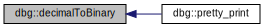
\includegraphics[width=336pt]{namespacedbg_acbbd001b36aaa78716ea7d9d2aeb3e46_icgraph}
\end{center}
\end{figure}
\mbox{\Hypertarget{namespacedbg_a20edc7ca4e92e4b3bddc6b983384aa00}\label{namespacedbg_a20edc7ca4e92e4b3bddc6b983384aa00}} 
\index{dbg@{dbg}!get\+\_\+type\+\_\+name@{get\+\_\+type\+\_\+name}}
\index{get\+\_\+type\+\_\+name@{get\+\_\+type\+\_\+name}!dbg@{dbg}}
\subsubsection{\texorpdfstring{get\+\_\+type\+\_\+name()}{get\_type\_name()}\hspace{0.1cm}{\footnotesize\ttfamily [1/10]}}
{\footnotesize\ttfamily template$<$int \&... Explicit\+Argument\+Barrier, typename T $>$ \\
std\+::string dbg\+::get\+\_\+type\+\_\+name (\begin{DoxyParamCaption}\item[{\hyperlink{structdbg_1_1type__tag}{type\+\_\+tag}$<$ T $>$}]{ }\end{DoxyParamCaption})}

Here is the call graph for this function\+:
\nopagebreak
\begin{figure}[H]
\begin{center}
\leavevmode
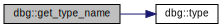
\includegraphics[width=294pt]{namespacedbg_a20edc7ca4e92e4b3bddc6b983384aa00_cgraph}
\end{center}
\end{figure}
Here is the caller graph for this function\+:
\nopagebreak
\begin{figure}[H]
\begin{center}
\leavevmode
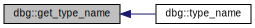
\includegraphics[width=327pt]{namespacedbg_a20edc7ca4e92e4b3bddc6b983384aa00_icgraph}
\end{center}
\end{figure}
\mbox{\Hypertarget{namespacedbg_a77b693006b8b158eb9a4604fba56a782}\label{namespacedbg_a77b693006b8b158eb9a4604fba56a782}} 
\index{dbg@{dbg}!get\+\_\+type\+\_\+name@{get\+\_\+type\+\_\+name}}
\index{get\+\_\+type\+\_\+name@{get\+\_\+type\+\_\+name}!dbg@{dbg}}
\subsubsection{\texorpdfstring{get\+\_\+type\+\_\+name()}{get\_type\_name()}\hspace{0.1cm}{\footnotesize\ttfamily [2/10]}}
{\footnotesize\ttfamily std\+::string dbg\+::get\+\_\+type\+\_\+name (\begin{DoxyParamCaption}\item[{\hyperlink{structdbg_1_1type__tag}{type\+\_\+tag}$<$ short $>$}]{ }\end{DoxyParamCaption})\hspace{0.3cm}{\ttfamily [inline]}}

\mbox{\Hypertarget{namespacedbg_ae70efee8c9a9d398975f71b216602097}\label{namespacedbg_ae70efee8c9a9d398975f71b216602097}} 
\index{dbg@{dbg}!get\+\_\+type\+\_\+name@{get\+\_\+type\+\_\+name}}
\index{get\+\_\+type\+\_\+name@{get\+\_\+type\+\_\+name}!dbg@{dbg}}
\subsubsection{\texorpdfstring{get\+\_\+type\+\_\+name()}{get\_type\_name()}\hspace{0.1cm}{\footnotesize\ttfamily [3/10]}}
{\footnotesize\ttfamily std\+::string dbg\+::get\+\_\+type\+\_\+name (\begin{DoxyParamCaption}\item[{\hyperlink{structdbg_1_1type__tag}{type\+\_\+tag}$<$ unsigned short $>$}]{ }\end{DoxyParamCaption})\hspace{0.3cm}{\ttfamily [inline]}}

\mbox{\Hypertarget{namespacedbg_a380f1bf409dda5e8c67a269b27d14aee}\label{namespacedbg_a380f1bf409dda5e8c67a269b27d14aee}} 
\index{dbg@{dbg}!get\+\_\+type\+\_\+name@{get\+\_\+type\+\_\+name}}
\index{get\+\_\+type\+\_\+name@{get\+\_\+type\+\_\+name}!dbg@{dbg}}
\subsubsection{\texorpdfstring{get\+\_\+type\+\_\+name()}{get\_type\_name()}\hspace{0.1cm}{\footnotesize\ttfamily [4/10]}}
{\footnotesize\ttfamily std\+::string dbg\+::get\+\_\+type\+\_\+name (\begin{DoxyParamCaption}\item[{\hyperlink{structdbg_1_1type__tag}{type\+\_\+tag}$<$ long $>$}]{ }\end{DoxyParamCaption})\hspace{0.3cm}{\ttfamily [inline]}}

\mbox{\Hypertarget{namespacedbg_a5316d9f58e72c20cfbb14496326d89f1}\label{namespacedbg_a5316d9f58e72c20cfbb14496326d89f1}} 
\index{dbg@{dbg}!get\+\_\+type\+\_\+name@{get\+\_\+type\+\_\+name}}
\index{get\+\_\+type\+\_\+name@{get\+\_\+type\+\_\+name}!dbg@{dbg}}
\subsubsection{\texorpdfstring{get\+\_\+type\+\_\+name()}{get\_type\_name()}\hspace{0.1cm}{\footnotesize\ttfamily [5/10]}}
{\footnotesize\ttfamily std\+::string dbg\+::get\+\_\+type\+\_\+name (\begin{DoxyParamCaption}\item[{\hyperlink{structdbg_1_1type__tag}{type\+\_\+tag}$<$ unsigned long $>$}]{ }\end{DoxyParamCaption})\hspace{0.3cm}{\ttfamily [inline]}}

\mbox{\Hypertarget{namespacedbg_a3bcf58cf4aba1da7a34e79b0fb2ce036}\label{namespacedbg_a3bcf58cf4aba1da7a34e79b0fb2ce036}} 
\index{dbg@{dbg}!get\+\_\+type\+\_\+name@{get\+\_\+type\+\_\+name}}
\index{get\+\_\+type\+\_\+name@{get\+\_\+type\+\_\+name}!dbg@{dbg}}
\subsubsection{\texorpdfstring{get\+\_\+type\+\_\+name()}{get\_type\_name()}\hspace{0.1cm}{\footnotesize\ttfamily [6/10]}}
{\footnotesize\ttfamily std\+::string dbg\+::get\+\_\+type\+\_\+name (\begin{DoxyParamCaption}\item[{\hyperlink{structdbg_1_1type__tag}{type\+\_\+tag}$<$ std\+::string $>$}]{ }\end{DoxyParamCaption})\hspace{0.3cm}{\ttfamily [inline]}}

\mbox{\Hypertarget{namespacedbg_a09680fe23089b62fd2879bd1f38897a6}\label{namespacedbg_a09680fe23089b62fd2879bd1f38897a6}} 
\index{dbg@{dbg}!get\+\_\+type\+\_\+name@{get\+\_\+type\+\_\+name}}
\index{get\+\_\+type\+\_\+name@{get\+\_\+type\+\_\+name}!dbg@{dbg}}
\subsubsection{\texorpdfstring{get\+\_\+type\+\_\+name()}{get\_type\_name()}\hspace{0.1cm}{\footnotesize\ttfamily [7/10]}}
{\footnotesize\ttfamily template$<$typename T $>$ \\
std\+::string dbg\+::get\+\_\+type\+\_\+name (\begin{DoxyParamCaption}\item[{\hyperlink{structdbg_1_1type__tag}{type\+\_\+tag}$<$ std\+::vector$<$ T, std\+::allocator$<$ T $>$$>$$>$}]{ }\end{DoxyParamCaption})}

\mbox{\Hypertarget{namespacedbg_aa4daf4ad755b0a3b4206debc162f064d}\label{namespacedbg_aa4daf4ad755b0a3b4206debc162f064d}} 
\index{dbg@{dbg}!get\+\_\+type\+\_\+name@{get\+\_\+type\+\_\+name}}
\index{get\+\_\+type\+\_\+name@{get\+\_\+type\+\_\+name}!dbg@{dbg}}
\subsubsection{\texorpdfstring{get\+\_\+type\+\_\+name()}{get\_type\_name()}\hspace{0.1cm}{\footnotesize\ttfamily [8/10]}}
{\footnotesize\ttfamily template$<$typename T1 , typename T2 $>$ \\
std\+::string dbg\+::get\+\_\+type\+\_\+name (\begin{DoxyParamCaption}\item[{\hyperlink{structdbg_1_1type__tag}{type\+\_\+tag}$<$ std\+::pair$<$ T1, T2 $>$$>$}]{ }\end{DoxyParamCaption})}

\mbox{\Hypertarget{namespacedbg_a1d187f8063d8c8c024e57a7985bcac78}\label{namespacedbg_a1d187f8063d8c8c024e57a7985bcac78}} 
\index{dbg@{dbg}!get\+\_\+type\+\_\+name@{get\+\_\+type\+\_\+name}}
\index{get\+\_\+type\+\_\+name@{get\+\_\+type\+\_\+name}!dbg@{dbg}}
\subsubsection{\texorpdfstring{get\+\_\+type\+\_\+name()}{get\_type\_name()}\hspace{0.1cm}{\footnotesize\ttfamily [9/10]}}
{\footnotesize\ttfamily template$<$typename... T$>$ \\
std\+::string dbg\+::get\+\_\+type\+\_\+name (\begin{DoxyParamCaption}\item[{\hyperlink{structdbg_1_1type__tag}{type\+\_\+tag}$<$ std\+::tuple$<$ T... $>$$>$}]{ }\end{DoxyParamCaption})}

Here is the call graph for this function\+:
\nopagebreak
\begin{figure}[H]
\begin{center}
\leavevmode
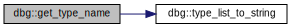
\includegraphics[width=350pt]{namespacedbg_a1d187f8063d8c8c024e57a7985bcac78_cgraph}
\end{center}
\end{figure}
\mbox{\Hypertarget{namespacedbg_a6224c816a1c695160e869f427854d569}\label{namespacedbg_a6224c816a1c695160e869f427854d569}} 
\index{dbg@{dbg}!get\+\_\+type\+\_\+name@{get\+\_\+type\+\_\+name}}
\index{get\+\_\+type\+\_\+name@{get\+\_\+type\+\_\+name}!dbg@{dbg}}
\subsubsection{\texorpdfstring{get\+\_\+type\+\_\+name()}{get\_type\_name()}\hspace{0.1cm}{\footnotesize\ttfamily [10/10]}}
{\footnotesize\ttfamily template$<$typename T $>$ \\
std\+::string dbg\+::get\+\_\+type\+\_\+name (\begin{DoxyParamCaption}\item[{\hyperlink{structdbg_1_1type__tag}{type\+\_\+tag}$<$ \hyperlink{structdbg_1_1print__formatted}{print\+\_\+formatted}$<$ T $>$$>$}]{ }\end{DoxyParamCaption})\hspace{0.3cm}{\ttfamily [inline]}}

\mbox{\Hypertarget{namespacedbg_afe9f0e1588144f8bb978cdc78d346682}\label{namespacedbg_afe9f0e1588144f8bb978cdc78d346682}} 
\index{dbg@{dbg}!hex@{hex}}
\index{hex@{hex}!dbg@{dbg}}
\subsubsection{\texorpdfstring{hex()}{hex()}}
{\footnotesize\ttfamily template$<$typename T $>$ \\
\hyperlink{structdbg_1_1print__formatted}{print\+\_\+formatted}$<$T$>$ dbg\+::hex (\begin{DoxyParamCaption}\item[{T}]{value }\end{DoxyParamCaption})}

Here is the caller graph for this function\+:
\nopagebreak
\begin{figure}[H]
\begin{center}
\leavevmode
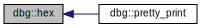
\includegraphics[width=273pt]{namespacedbg_afe9f0e1588144f8bb978cdc78d346682_icgraph}
\end{center}
\end{figure}
\mbox{\Hypertarget{namespacedbg_a23f10decf1edf2d34e226437e5562452}\label{namespacedbg_a23f10decf1edf2d34e226437e5562452}} 
\index{dbg@{dbg}!identity@{identity}}
\index{identity@{identity}!dbg@{dbg}}
\subsubsection{\texorpdfstring{identity()}{identity()}}
{\footnotesize\ttfamily template$<$typename T $>$ \\
T\&\& dbg\+::identity (\begin{DoxyParamCaption}\item[{T \&\&}]{t }\end{DoxyParamCaption})}

\mbox{\Hypertarget{namespacedbg_a4dffa8fa9b0dd86306608691d534a050}\label{namespacedbg_a4dffa8fa9b0dd86306608691d534a050}} 
\index{dbg@{dbg}!is\+Colorized\+Output\+Enabled@{is\+Colorized\+Output\+Enabled}}
\index{is\+Colorized\+Output\+Enabled@{is\+Colorized\+Output\+Enabled}!dbg@{dbg}}
\subsubsection{\texorpdfstring{is\+Colorized\+Output\+Enabled()}{isColorizedOutputEnabled()}}
{\footnotesize\ttfamily bool dbg\+::is\+Colorized\+Output\+Enabled (\begin{DoxyParamCaption}{ }\end{DoxyParamCaption})\hspace{0.3cm}{\ttfamily [inline]}}

\mbox{\Hypertarget{namespacedbg_af52f01dbdbb25506c5cfecab4c57d52a}\label{namespacedbg_af52f01dbdbb25506c5cfecab4c57d52a}} 
\index{dbg@{dbg}!oct@{oct}}
\index{oct@{oct}!dbg@{dbg}}
\subsubsection{\texorpdfstring{oct()}{oct()}}
{\footnotesize\ttfamily template$<$typename T $>$ \\
\hyperlink{structdbg_1_1print__formatted}{print\+\_\+formatted}$<$T$>$ dbg\+::oct (\begin{DoxyParamCaption}\item[{T}]{value }\end{DoxyParamCaption})}

\mbox{\Hypertarget{namespacedbg_a4ba5b016ce65b09fef3935a945310904}\label{namespacedbg_a4ba5b016ce65b09fef3935a945310904}} 
\index{dbg@{dbg}!pretty\+\_\+print@{pretty\+\_\+print}}
\index{pretty\+\_\+print@{pretty\+\_\+print}!dbg@{dbg}}
\subsubsection{\texorpdfstring{pretty\+\_\+print()}{pretty\_print()}\hspace{0.1cm}{\footnotesize\ttfamily [1/19]}}
{\footnotesize\ttfamily template$<$typename T $>$ \\
void dbg\+::pretty\+\_\+print (\begin{DoxyParamCaption}\item[{std\+::ostream \&}]{stream,  }\item[{const T \&}]{value,  }\item[{std\+::true\+\_\+type}]{ }\end{DoxyParamCaption})\hspace{0.3cm}{\ttfamily [inline]}}

Here is the caller graph for this function\+:
\nopagebreak
\begin{figure}[H]
\begin{center}
\leavevmode
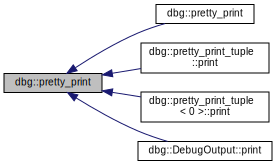
\includegraphics[width=348pt]{namespacedbg_a4ba5b016ce65b09fef3935a945310904_icgraph}
\end{center}
\end{figure}
\mbox{\Hypertarget{namespacedbg_ab875770941388a1d8279e9b5257e5a93}\label{namespacedbg_ab875770941388a1d8279e9b5257e5a93}} 
\index{dbg@{dbg}!pretty\+\_\+print@{pretty\+\_\+print}}
\index{pretty\+\_\+print@{pretty\+\_\+print}!dbg@{dbg}}
\subsubsection{\texorpdfstring{pretty\+\_\+print()}{pretty\_print()}\hspace{0.1cm}{\footnotesize\ttfamily [2/19]}}
{\footnotesize\ttfamily template$<$typename T $>$ \\
void dbg\+::pretty\+\_\+print (\begin{DoxyParamCaption}\item[{std\+::ostream \&}]{,  }\item[{const T \&}]{,  }\item[{std\+::false\+\_\+type}]{ }\end{DoxyParamCaption})\hspace{0.3cm}{\ttfamily [inline]}}

Here is the call graph for this function\+:
\nopagebreak
\begin{figure}[H]
\begin{center}
\leavevmode
\includegraphics[width=276pt]{namespacedbg_ab875770941388a1d8279e9b5257e5a93_cgraph}
\end{center}
\end{figure}
\mbox{\Hypertarget{namespacedbg_a4920208faa7096e0333f9d14119a9c2f}\label{namespacedbg_a4920208faa7096e0333f9d14119a9c2f}} 
\index{dbg@{dbg}!pretty\+\_\+print@{pretty\+\_\+print}}
\index{pretty\+\_\+print@{pretty\+\_\+print}!dbg@{dbg}}
\subsubsection{\texorpdfstring{pretty\+\_\+print()}{pretty\_print()}\hspace{0.1cm}{\footnotesize\ttfamily [3/19]}}
{\footnotesize\ttfamily template$<$typename T $>$ \\
std\+::enable\+\_\+if$<$!\hyperlink{structdbg_1_1detail_1_1is__container}{detail\+::is\+\_\+container}$<$const T\&$>$\+::value \&\& !std\+::is\+\_\+enum$<$T$>$\+::value, bool$>$\+::\hyperlink{namespacedbg_a2365d80e3a3525e6025040383ff8661b}{type} dbg\+::pretty\+\_\+print (\begin{DoxyParamCaption}\item[{std\+::ostream \&}]{stream,  }\item[{const T \&}]{value }\end{DoxyParamCaption})\hspace{0.3cm}{\ttfamily [inline]}}

Here is the call graph for this function\+:
\nopagebreak
\begin{figure}[H]
\begin{center}
\leavevmode
\includegraphics[width=312pt]{namespacedbg_a4920208faa7096e0333f9d14119a9c2f_cgraph}
\end{center}
\end{figure}
\mbox{\Hypertarget{namespacedbg_a4f9989bfef507d5034cc50d015654ca4}\label{namespacedbg_a4f9989bfef507d5034cc50d015654ca4}} 
\index{dbg@{dbg}!pretty\+\_\+print@{pretty\+\_\+print}}
\index{pretty\+\_\+print@{pretty\+\_\+print}!dbg@{dbg}}
\subsubsection{\texorpdfstring{pretty\+\_\+print()}{pretty\_print()}\hspace{0.1cm}{\footnotesize\ttfamily [4/19]}}
{\footnotesize\ttfamily bool dbg\+::pretty\+\_\+print (\begin{DoxyParamCaption}\item[{std\+::ostream \&}]{stream,  }\item[{const bool \&}]{value }\end{DoxyParamCaption})\hspace{0.3cm}{\ttfamily [inline]}}

\mbox{\Hypertarget{namespacedbg_acc6a678f0c3954671e247468e249e5a4}\label{namespacedbg_acc6a678f0c3954671e247468e249e5a4}} 
\index{dbg@{dbg}!pretty\+\_\+print@{pretty\+\_\+print}}
\index{pretty\+\_\+print@{pretty\+\_\+print}!dbg@{dbg}}
\subsubsection{\texorpdfstring{pretty\+\_\+print()}{pretty\_print()}\hspace{0.1cm}{\footnotesize\ttfamily [5/19]}}
{\footnotesize\ttfamily bool dbg\+::pretty\+\_\+print (\begin{DoxyParamCaption}\item[{std\+::ostream \&}]{stream,  }\item[{const char \&}]{value }\end{DoxyParamCaption})\hspace{0.3cm}{\ttfamily [inline]}}

Here is the call graph for this function\+:
\nopagebreak
\begin{figure}[H]
\begin{center}
\leavevmode
\includegraphics[width=273pt]{namespacedbg_acc6a678f0c3954671e247468e249e5a4_cgraph}
\end{center}
\end{figure}
\mbox{\Hypertarget{namespacedbg_a2194ca6a2105fd8c57e5cb43f688d240}\label{namespacedbg_a2194ca6a2105fd8c57e5cb43f688d240}} 
\index{dbg@{dbg}!pretty\+\_\+print@{pretty\+\_\+print}}
\index{pretty\+\_\+print@{pretty\+\_\+print}!dbg@{dbg}}
\subsubsection{\texorpdfstring{pretty\+\_\+print()}{pretty\_print()}\hspace{0.1cm}{\footnotesize\ttfamily [6/19]}}
{\footnotesize\ttfamily template$<$typename P $>$ \\
bool dbg\+::pretty\+\_\+print (\begin{DoxyParamCaption}\item[{std\+::ostream \&}]{stream,  }\item[{P $\ast$const \&}]{value }\end{DoxyParamCaption})\hspace{0.3cm}{\ttfamily [inline]}}

\mbox{\Hypertarget{namespacedbg_a6cbcb99c1fdd640925d80c390af3954a}\label{namespacedbg_a6cbcb99c1fdd640925d80c390af3954a}} 
\index{dbg@{dbg}!pretty\+\_\+print@{pretty\+\_\+print}}
\index{pretty\+\_\+print@{pretty\+\_\+print}!dbg@{dbg}}
\subsubsection{\texorpdfstring{pretty\+\_\+print()}{pretty\_print()}\hspace{0.1cm}{\footnotesize\ttfamily [7/19]}}
{\footnotesize\ttfamily template$<$typename T , typename Deleter $>$ \\
bool dbg\+::pretty\+\_\+print (\begin{DoxyParamCaption}\item[{std\+::ostream \&}]{stream,  }\item[{std\+::unique\+\_\+ptr$<$ T, Deleter $>$ \&}]{value }\end{DoxyParamCaption})\hspace{0.3cm}{\ttfamily [inline]}}

Here is the call graph for this function\+:
\nopagebreak
\begin{figure}[H]
\begin{center}
\leavevmode
\includegraphics[width=312pt]{namespacedbg_a6cbcb99c1fdd640925d80c390af3954a_cgraph}
\end{center}
\end{figure}
\mbox{\Hypertarget{namespacedbg_ae36a726fc12c4b6c13878e051f4f3ad7}\label{namespacedbg_ae36a726fc12c4b6c13878e051f4f3ad7}} 
\index{dbg@{dbg}!pretty\+\_\+print@{pretty\+\_\+print}}
\index{pretty\+\_\+print@{pretty\+\_\+print}!dbg@{dbg}}
\subsubsection{\texorpdfstring{pretty\+\_\+print()}{pretty\_print()}\hspace{0.1cm}{\footnotesize\ttfamily [8/19]}}
{\footnotesize\ttfamily template$<$typename T $>$ \\
bool dbg\+::pretty\+\_\+print (\begin{DoxyParamCaption}\item[{std\+::ostream \&}]{stream,  }\item[{std\+::shared\+\_\+ptr$<$ T $>$ \&}]{value }\end{DoxyParamCaption})\hspace{0.3cm}{\ttfamily [inline]}}

Here is the call graph for this function\+:
\nopagebreak
\begin{figure}[H]
\begin{center}
\leavevmode
\includegraphics[width=312pt]{namespacedbg_ae36a726fc12c4b6c13878e051f4f3ad7_cgraph}
\end{center}
\end{figure}
\mbox{\Hypertarget{namespacedbg_adb407af036065563d2e8ef131305475a}\label{namespacedbg_adb407af036065563d2e8ef131305475a}} 
\index{dbg@{dbg}!pretty\+\_\+print@{pretty\+\_\+print}}
\index{pretty\+\_\+print@{pretty\+\_\+print}!dbg@{dbg}}
\subsubsection{\texorpdfstring{pretty\+\_\+print()}{pretty\_print()}\hspace{0.1cm}{\footnotesize\ttfamily [9/19]}}
{\footnotesize\ttfamily template$<$size\+\_\+t N$>$ \\
bool dbg\+::pretty\+\_\+print (\begin{DoxyParamCaption}\item[{std\+::ostream \&}]{stream,  }\item[{const char(\&)}]{value\mbox{[}\+N\mbox{]} }\end{DoxyParamCaption})\hspace{0.3cm}{\ttfamily [inline]}}

\mbox{\Hypertarget{namespacedbg_a17cebbee60948a473318356a59d7f825}\label{namespacedbg_a17cebbee60948a473318356a59d7f825}} 
\index{dbg@{dbg}!pretty\+\_\+print@{pretty\+\_\+print}}
\index{pretty\+\_\+print@{pretty\+\_\+print}!dbg@{dbg}}
\subsubsection{\texorpdfstring{pretty\+\_\+print()}{pretty\_print()}\hspace{0.1cm}{\footnotesize\ttfamily [10/19]}}
{\footnotesize\ttfamily template$<$$>$ \\
bool dbg\+::pretty\+\_\+print (\begin{DoxyParamCaption}\item[{std\+::ostream \&}]{stream,  }\item[{const char $\ast$const \&}]{value }\end{DoxyParamCaption})\hspace{0.3cm}{\ttfamily [inline]}}

\mbox{\Hypertarget{namespacedbg_a48e38a2e7f91709c4eac1c3ff1532f35}\label{namespacedbg_a48e38a2e7f91709c4eac1c3ff1532f35}} 
\index{dbg@{dbg}!pretty\+\_\+print@{pretty\+\_\+print}}
\index{pretty\+\_\+print@{pretty\+\_\+print}!dbg@{dbg}}
\subsubsection{\texorpdfstring{pretty\+\_\+print()}{pretty\_print()}\hspace{0.1cm}{\footnotesize\ttfamily [11/19]}}
{\footnotesize\ttfamily template$<$typename... Ts$>$ \\
bool dbg\+::pretty\+\_\+print (\begin{DoxyParamCaption}\item[{std\+::ostream \&}]{stream,  }\item[{const std\+::tuple$<$ Ts... $>$ \&}]{value }\end{DoxyParamCaption})\hspace{0.3cm}{\ttfamily [inline]}}

\mbox{\Hypertarget{namespacedbg_a077f3d4254963a89c600b07eb1b8608b}\label{namespacedbg_a077f3d4254963a89c600b07eb1b8608b}} 
\index{dbg@{dbg}!pretty\+\_\+print@{pretty\+\_\+print}}
\index{pretty\+\_\+print@{pretty\+\_\+print}!dbg@{dbg}}
\subsubsection{\texorpdfstring{pretty\+\_\+print()}{pretty\_print()}\hspace{0.1cm}{\footnotesize\ttfamily [12/19]}}
{\footnotesize\ttfamily template$<$$>$ \\
bool dbg\+::pretty\+\_\+print (\begin{DoxyParamCaption}\item[{std\+::ostream \&}]{stream,  }\item[{const std\+::tuple$<$$>$ \&}]{ }\end{DoxyParamCaption})\hspace{0.3cm}{\ttfamily [inline]}}

\mbox{\Hypertarget{namespacedbg_a43fb1da62bd4a702ea7ca37e665c53c9}\label{namespacedbg_a43fb1da62bd4a702ea7ca37e665c53c9}} 
\index{dbg@{dbg}!pretty\+\_\+print@{pretty\+\_\+print}}
\index{pretty\+\_\+print@{pretty\+\_\+print}!dbg@{dbg}}
\subsubsection{\texorpdfstring{pretty\+\_\+print()}{pretty\_print()}\hspace{0.1cm}{\footnotesize\ttfamily [13/19]}}
{\footnotesize\ttfamily template$<$$>$ \\
bool dbg\+::pretty\+\_\+print (\begin{DoxyParamCaption}\item[{std\+::ostream \&}]{stream,  }\item[{const \hyperlink{structdbg_1_1time}{time} \&}]{ }\end{DoxyParamCaption})\hspace{0.3cm}{\ttfamily [inline]}}

\mbox{\Hypertarget{namespacedbg_a3f0682f5939ac9a18ba7ee86a5c63243}\label{namespacedbg_a3f0682f5939ac9a18ba7ee86a5c63243}} 
\index{dbg@{dbg}!pretty\+\_\+print@{pretty\+\_\+print}}
\index{pretty\+\_\+print@{pretty\+\_\+print}!dbg@{dbg}}
\subsubsection{\texorpdfstring{pretty\+\_\+print()}{pretty\_print()}\hspace{0.1cm}{\footnotesize\ttfamily [14/19]}}
{\footnotesize\ttfamily template$<$typename T $>$ \\
bool dbg\+::pretty\+\_\+print (\begin{DoxyParamCaption}\item[{std\+::ostream \&}]{stream,  }\item[{const \hyperlink{structdbg_1_1print__formatted}{print\+\_\+formatted}$<$ T $>$ \&}]{value }\end{DoxyParamCaption})\hspace{0.3cm}{\ttfamily [inline]}}

Here is the call graph for this function\+:
\nopagebreak
\begin{figure}[H]
\begin{center}
\leavevmode
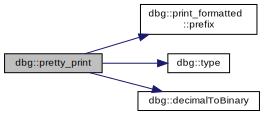
\includegraphics[width=336pt]{namespacedbg_a3f0682f5939ac9a18ba7ee86a5c63243_cgraph}
\end{center}
\end{figure}
\mbox{\Hypertarget{namespacedbg_abb85fb70314b6ada2e66eebeafcd15bf}\label{namespacedbg_abb85fb70314b6ada2e66eebeafcd15bf}} 
\index{dbg@{dbg}!pretty\+\_\+print@{pretty\+\_\+print}}
\index{pretty\+\_\+print@{pretty\+\_\+print}!dbg@{dbg}}
\subsubsection{\texorpdfstring{pretty\+\_\+print()}{pretty\_print()}\hspace{0.1cm}{\footnotesize\ttfamily [15/19]}}
{\footnotesize\ttfamily template$<$typename T $>$ \\
bool dbg\+::pretty\+\_\+print (\begin{DoxyParamCaption}\item[{std\+::ostream \&}]{stream,  }\item[{const \hyperlink{structdbg_1_1print__type}{print\+\_\+type}$<$ T $>$ \&}]{ }\end{DoxyParamCaption})\hspace{0.3cm}{\ttfamily [inline]}}

Here is the call graph for this function\+:
\nopagebreak
\begin{figure}[H]
\begin{center}
\leavevmode
\includegraphics[width=276pt]{namespacedbg_abb85fb70314b6ada2e66eebeafcd15bf_cgraph}
\end{center}
\end{figure}
\mbox{\Hypertarget{namespacedbg_a1212dc990d58f20efcf5d66eb4a5781c}\label{namespacedbg_a1212dc990d58f20efcf5d66eb4a5781c}} 
\index{dbg@{dbg}!pretty\+\_\+print@{pretty\+\_\+print}}
\index{pretty\+\_\+print@{pretty\+\_\+print}!dbg@{dbg}}
\subsubsection{\texorpdfstring{pretty\+\_\+print()}{pretty\_print()}\hspace{0.1cm}{\footnotesize\ttfamily [16/19]}}
{\footnotesize\ttfamily template$<$typename Container $>$ \\
std\+::enable\+\_\+if$<$\hyperlink{structdbg_1_1detail_1_1is__container}{detail\+::is\+\_\+container}$<$const Container\&$>$\+::value, bool$>$\+::\hyperlink{namespacedbg_a2365d80e3a3525e6025040383ff8661b}{type} dbg\+::pretty\+\_\+print (\begin{DoxyParamCaption}\item[{std\+::ostream \&}]{stream,  }\item[{const Container \&}]{value }\end{DoxyParamCaption})\hspace{0.3cm}{\ttfamily [inline]}}

Here is the call graph for this function\+:
\nopagebreak
\begin{figure}[H]
\begin{center}
\leavevmode
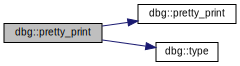
\includegraphics[width=312pt]{namespacedbg_a1212dc990d58f20efcf5d66eb4a5781c_cgraph}
\end{center}
\end{figure}
\mbox{\Hypertarget{namespacedbg_acd3034b7476cdf474e46eb2bbca6e0d1}\label{namespacedbg_acd3034b7476cdf474e46eb2bbca6e0d1}} 
\index{dbg@{dbg}!pretty\+\_\+print@{pretty\+\_\+print}}
\index{pretty\+\_\+print@{pretty\+\_\+print}!dbg@{dbg}}
\subsubsection{\texorpdfstring{pretty\+\_\+print()}{pretty\_print()}\hspace{0.1cm}{\footnotesize\ttfamily [17/19]}}
{\footnotesize\ttfamily template$<$typename Enum $>$ \\
std\+::enable\+\_\+if$<$std\+::is\+\_\+enum$<$Enum$>$\+::value, bool$>$\+::\hyperlink{namespacedbg_a2365d80e3a3525e6025040383ff8661b}{type} dbg\+::pretty\+\_\+print (\begin{DoxyParamCaption}\item[{std\+::ostream \&}]{stream,  }\item[{Enum const \&}]{value }\end{DoxyParamCaption})\hspace{0.3cm}{\ttfamily [inline]}}

Here is the call graph for this function\+:
\nopagebreak
\begin{figure}[H]
\begin{center}
\leavevmode
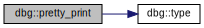
\includegraphics[width=276pt]{namespacedbg_acd3034b7476cdf474e46eb2bbca6e0d1_cgraph}
\end{center}
\end{figure}
\mbox{\Hypertarget{namespacedbg_ae620aa6031e088dc11e1df853e38f5fa}\label{namespacedbg_ae620aa6031e088dc11e1df853e38f5fa}} 
\index{dbg@{dbg}!pretty\+\_\+print@{pretty\+\_\+print}}
\index{pretty\+\_\+print@{pretty\+\_\+print}!dbg@{dbg}}
\subsubsection{\texorpdfstring{pretty\+\_\+print()}{pretty\_print()}\hspace{0.1cm}{\footnotesize\ttfamily [18/19]}}
{\footnotesize\ttfamily bool dbg\+::pretty\+\_\+print (\begin{DoxyParamCaption}\item[{std\+::ostream \&}]{stream,  }\item[{const std\+::string \&}]{value }\end{DoxyParamCaption})\hspace{0.3cm}{\ttfamily [inline]}}

\mbox{\Hypertarget{namespacedbg_adf02078069da78815c208dd638a01640}\label{namespacedbg_adf02078069da78815c208dd638a01640}} 
\index{dbg@{dbg}!pretty\+\_\+print@{pretty\+\_\+print}}
\index{pretty\+\_\+print@{pretty\+\_\+print}!dbg@{dbg}}
\subsubsection{\texorpdfstring{pretty\+\_\+print()}{pretty\_print()}\hspace{0.1cm}{\footnotesize\ttfamily [19/19]}}
{\footnotesize\ttfamily template$<$typename T1 , typename T2 $>$ \\
bool dbg\+::pretty\+\_\+print (\begin{DoxyParamCaption}\item[{std\+::ostream \&}]{stream,  }\item[{const std\+::pair$<$ T1, T2 $>$ \&}]{value }\end{DoxyParamCaption})\hspace{0.3cm}{\ttfamily [inline]}}

Here is the call graph for this function\+:
\nopagebreak
\begin{figure}[H]
\begin{center}
\leavevmode
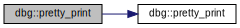
\includegraphics[width=312pt]{namespacedbg_adf02078069da78815c208dd638a01640_cgraph}
\end{center}
\end{figure}
\mbox{\Hypertarget{namespacedbg_a2365d80e3a3525e6025040383ff8661b}\label{namespacedbg_a2365d80e3a3525e6025040383ff8661b}} 
\index{dbg@{dbg}!type@{type}}
\index{type@{type}!dbg@{dbg}}
\subsubsection{\texorpdfstring{type()}{type()}}
{\footnotesize\ttfamily template$<$typename T $>$ \\
\hyperlink{structdbg_1_1print__type}{print\+\_\+type}$<$T$>$ dbg\+::type (\begin{DoxyParamCaption}{ }\end{DoxyParamCaption})}

Here is the caller graph for this function\+:
\nopagebreak
\begin{figure}[H]
\begin{center}
\leavevmode
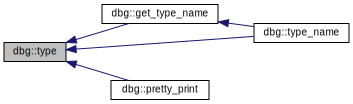
\includegraphics[width=350pt]{namespacedbg_a2365d80e3a3525e6025040383ff8661b_icgraph}
\end{center}
\end{figure}
\mbox{\Hypertarget{namespacedbg_aef0097e53230ee373eaabc4981048cac}\label{namespacedbg_aef0097e53230ee373eaabc4981048cac}} 
\index{dbg@{dbg}!type\+\_\+list\+\_\+to\+\_\+string@{type\+\_\+list\+\_\+to\+\_\+string}}
\index{type\+\_\+list\+\_\+to\+\_\+string@{type\+\_\+list\+\_\+to\+\_\+string}!dbg@{dbg}}
\subsubsection{\texorpdfstring{type\+\_\+list\+\_\+to\+\_\+string()}{type\_list\_to\_string()}}
{\footnotesize\ttfamily template$<$typename... T$>$ \\
std\+::string dbg\+::type\+\_\+list\+\_\+to\+\_\+string (\begin{DoxyParamCaption}{ }\end{DoxyParamCaption})}

Here is the caller graph for this function\+:
\nopagebreak
\begin{figure}[H]
\begin{center}
\leavevmode
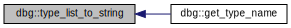
\includegraphics[width=350pt]{namespacedbg_aef0097e53230ee373eaabc4981048cac_icgraph}
\end{center}
\end{figure}
\mbox{\Hypertarget{namespacedbg_aab63fa619583229308f148088ffac7a0}\label{namespacedbg_aab63fa619583229308f148088ffac7a0}} 
\index{dbg@{dbg}!type\+\_\+name@{type\+\_\+name}}
\index{type\+\_\+name@{type\+\_\+name}!dbg@{dbg}}
\subsubsection{\texorpdfstring{type\+\_\+name()}{type\_name()}}
{\footnotesize\ttfamily template$<$typename T $>$ \\
std\+::string dbg\+::type\+\_\+name (\begin{DoxyParamCaption}{ }\end{DoxyParamCaption})}

Here is the call graph for this function\+:
\nopagebreak
\begin{figure}[H]
\begin{center}
\leavevmode
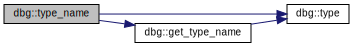
\includegraphics[width=350pt]{namespacedbg_aab63fa619583229308f148088ffac7a0_cgraph}
\end{center}
\end{figure}
\mbox{\Hypertarget{namespacedbg_aaf90b7c26aa95f1666f2446996973cac}\label{namespacedbg_aaf90b7c26aa95f1666f2446996973cac}} 
\index{dbg@{dbg}!type\+\_\+name\+\_\+impl@{type\+\_\+name\+\_\+impl}}
\index{type\+\_\+name\+\_\+impl@{type\+\_\+name\+\_\+impl}!dbg@{dbg}}
\subsubsection{\texorpdfstring{type\+\_\+name\+\_\+impl()}{type\_name\_impl()}}
{\footnotesize\ttfamily template$<$typename T $>$ \\
const char$\ast$ dbg\+::type\+\_\+name\+\_\+impl (\begin{DoxyParamCaption}{ }\end{DoxyParamCaption})}


\hypertarget{namespacedbg_1_1detail}{}\section{dbg\+:\+:detail Namespace Reference}
\label{namespacedbg_1_1detail}\index{dbg\+::detail@{dbg\+::detail}}
\subsection*{Classes}
\begin{DoxyCompactItemize}
\item 
struct \hyperlink{structdbg_1_1detail_1_1has__ostream__operator}{has\+\_\+ostream\+\_\+operator}
\item 
struct \hyperlink{structdbg_1_1detail_1_1is__container}{is\+\_\+container}
\end{DoxyCompactItemize}
\subsection*{Typedefs}
\begin{DoxyCompactItemize}
\item 
{\footnotesize template$<$typename T $>$ }\\using \hyperlink{namespacedbg_1_1detail_acfad41bd0b116575799b79d85fc5c883}{detect\+\_\+begin\+\_\+t} = decltype(detail\+::begin(std\+::declval$<$ T $>$()))
\item 
{\footnotesize template$<$typename T $>$ }\\using \hyperlink{namespacedbg_1_1detail_ab462e0c9e2d1686d323d638613692839}{detect\+\_\+end\+\_\+t} = decltype(detail\+::end(std\+::declval$<$ T $>$()))
\item 
{\footnotesize template$<$typename T $>$ }\\using \hyperlink{namespacedbg_1_1detail_a19adefcfcaddecb9f32e810ebcae4856}{detect\+\_\+size\+\_\+t} = decltype(detail\+::size(std\+::declval$<$ T $>$()))
\item 
{\footnotesize template$<$typename T $>$ }\\using \hyperlink{namespacedbg_1_1detail_a2c6a2bc0c8581b3b0d285d1d2971e44d}{ostream\+\_\+operator\+\_\+t} = decltype(std\+::declval$<$ std\+::ostream \& $>$()$<$$<$ std\+::declval$<$ T $>$())
\end{DoxyCompactItemize}


\subsection{Typedef Documentation}
\mbox{\Hypertarget{namespacedbg_1_1detail_acfad41bd0b116575799b79d85fc5c883}\label{namespacedbg_1_1detail_acfad41bd0b116575799b79d85fc5c883}} 
\index{dbg\+::detail@{dbg\+::detail}!detect\+\_\+begin\+\_\+t@{detect\+\_\+begin\+\_\+t}}
\index{detect\+\_\+begin\+\_\+t@{detect\+\_\+begin\+\_\+t}!dbg\+::detail@{dbg\+::detail}}
\subsubsection{\texorpdfstring{detect\+\_\+begin\+\_\+t}{detect\_begin\_t}}
{\footnotesize\ttfamily template$<$typename T $>$ \\
using \hyperlink{namespacedbg_1_1detail_acfad41bd0b116575799b79d85fc5c883}{dbg\+::detail\+::detect\+\_\+begin\+\_\+t} = typedef decltype(detail\+::begin(std\+::declval$<$T$>$()))}

\mbox{\Hypertarget{namespacedbg_1_1detail_ab462e0c9e2d1686d323d638613692839}\label{namespacedbg_1_1detail_ab462e0c9e2d1686d323d638613692839}} 
\index{dbg\+::detail@{dbg\+::detail}!detect\+\_\+end\+\_\+t@{detect\+\_\+end\+\_\+t}}
\index{detect\+\_\+end\+\_\+t@{detect\+\_\+end\+\_\+t}!dbg\+::detail@{dbg\+::detail}}
\subsubsection{\texorpdfstring{detect\+\_\+end\+\_\+t}{detect\_end\_t}}
{\footnotesize\ttfamily template$<$typename T $>$ \\
using \hyperlink{namespacedbg_1_1detail_ab462e0c9e2d1686d323d638613692839}{dbg\+::detail\+::detect\+\_\+end\+\_\+t} = typedef decltype(detail\+::end(std\+::declval$<$T$>$()))}

\mbox{\Hypertarget{namespacedbg_1_1detail_a19adefcfcaddecb9f32e810ebcae4856}\label{namespacedbg_1_1detail_a19adefcfcaddecb9f32e810ebcae4856}} 
\index{dbg\+::detail@{dbg\+::detail}!detect\+\_\+size\+\_\+t@{detect\+\_\+size\+\_\+t}}
\index{detect\+\_\+size\+\_\+t@{detect\+\_\+size\+\_\+t}!dbg\+::detail@{dbg\+::detail}}
\subsubsection{\texorpdfstring{detect\+\_\+size\+\_\+t}{detect\_size\_t}}
{\footnotesize\ttfamily template$<$typename T $>$ \\
using \hyperlink{namespacedbg_1_1detail_a19adefcfcaddecb9f32e810ebcae4856}{dbg\+::detail\+::detect\+\_\+size\+\_\+t} = typedef decltype(detail\+::size(std\+::declval$<$T$>$()))}

\mbox{\Hypertarget{namespacedbg_1_1detail_a2c6a2bc0c8581b3b0d285d1d2971e44d}\label{namespacedbg_1_1detail_a2c6a2bc0c8581b3b0d285d1d2971e44d}} 
\index{dbg\+::detail@{dbg\+::detail}!ostream\+\_\+operator\+\_\+t@{ostream\+\_\+operator\+\_\+t}}
\index{ostream\+\_\+operator\+\_\+t@{ostream\+\_\+operator\+\_\+t}!dbg\+::detail@{dbg\+::detail}}
\subsubsection{\texorpdfstring{ostream\+\_\+operator\+\_\+t}{ostream\_operator\_t}}
{\footnotesize\ttfamily template$<$typename T $>$ \\
using \hyperlink{namespacedbg_1_1detail_a2c6a2bc0c8581b3b0d285d1d2971e44d}{dbg\+::detail\+::ostream\+\_\+operator\+\_\+t} = typedef decltype(std\+::declval$<$std\+::ostream\&$>$() $<$$<$ std\+::declval$<$T$>$())}


\hypertarget{namespacedbg_1_1detail__detector}{}\section{dbg\+:\+:detail\+\_\+detector Namespace Reference}
\label{namespacedbg_1_1detail__detector}\index{dbg\+::detail\+\_\+detector@{dbg\+::detail\+\_\+detector}}
\subsection*{Classes}
\begin{DoxyCompactItemize}
\item 
struct \hyperlink{structdbg_1_1detail__detector_1_1detector}{detector}
\item 
struct \hyperlink{structdbg_1_1detail__detector_1_1detector_3_01_default_00_01void__t_3_01_op_3_01_args_8_8_8_01_4b82e02bb2aa06b0130d0ab9c715e6bdd}{detector$<$ Default, void\+\_\+t$<$ Op$<$ Args... $>$ $>$, Op, Args... $>$}
\item 
struct \hyperlink{structdbg_1_1detail__detector_1_1nonesuch}{nonesuch}
\end{DoxyCompactItemize}
\subsection*{Typedefs}
\begin{DoxyCompactItemize}
\item 
{\footnotesize template$<$typename... $>$ }\\using \hyperlink{namespacedbg_1_1detail__detector_a1dbadccf461338e71c55ea392d4ed47c}{void\+\_\+t} = void
\end{DoxyCompactItemize}


\subsection{Typedef Documentation}
\mbox{\Hypertarget{namespacedbg_1_1detail__detector_a1dbadccf461338e71c55ea392d4ed47c}\label{namespacedbg_1_1detail__detector_a1dbadccf461338e71c55ea392d4ed47c}} 
\index{dbg\+::detail\+\_\+detector@{dbg\+::detail\+\_\+detector}!void\+\_\+t@{void\+\_\+t}}
\index{void\+\_\+t@{void\+\_\+t}!dbg\+::detail\+\_\+detector@{dbg\+::detail\+\_\+detector}}
\subsubsection{\texorpdfstring{void\+\_\+t}{void\_t}}
{\footnotesize\ttfamily template$<$typename... $>$ \\
using \hyperlink{namespacedbg_1_1detail__detector_a1dbadccf461338e71c55ea392d4ed47c}{dbg\+::detail\+\_\+detector\+::void\+\_\+t} = typedef void}


\hypertarget{namespacedbg_1_1pretty__function}{}\section{dbg\+:\+:pretty\+\_\+function Namespace Reference}
\label{namespacedbg_1_1pretty__function}\index{dbg\+::pretty\+\_\+function@{dbg\+::pretty\+\_\+function}}

\hypertarget{namespacegame}{}\section{game Namespace Reference}
\label{namespacegame}\index{game@{game}}
\subsection*{Namespaces}
\begin{DoxyCompactItemize}
\item 
 \hyperlink{namespacegame_1_1penguin}{penguin}
\item 
 \hyperlink{namespacegame_1_1tic__tac__toe}{tic\+\_\+tac\+\_\+toe}
\end{DoxyCompactItemize}
\subsection*{Classes}
\begin{DoxyCompactItemize}
\item 
class \hyperlink{classgame_1_1_abstract_board}{Abstract\+Board}
\begin{DoxyCompactList}\small\item\em Describe the basics of a Board. \end{DoxyCompactList}\item 
class \hyperlink{classgame_1_1_abstract_board_cell}{Abstract\+Board\+Cell}
\item 
class \hyperlink{classgame_1_1_abstract_game}{Abstract\+Game}
\item 
class \hyperlink{classgame_1_1_abstract_interface}{Abstract\+Interface}
\item 
class \hyperlink{classgame_1_1_abstract_pawn}{Abstract\+Pawn}
\item 
class \hyperlink{classgame_1_1_abstract_player}{Abstract\+Player}
\item 
class \hyperlink{classgame_1_1_history}{History}
\item 
struct \hyperlink{structgame_1_1_move}{Move}
\item 
struct \hyperlink{structgame_1_1_position}{Position}
\item 
struct \hyperlink{structgame_1_1_position3_d}{Position3D}
\item 
struct \hyperlink{structgame_1_1position__3_d__hash__function}{position\+\_\+3\+D\+\_\+hash\+\_\+function}
\begin{DoxyCompactList}\small\item\em Proper hash function specialized for \hyperlink{structgame_1_1_position}{Position}. \end{DoxyCompactList}\item 
struct \hyperlink{structgame_1_1position__hash__function}{position\+\_\+hash\+\_\+function}
\begin{DoxyCompactList}\small\item\em Proper hash function specialized for \hyperlink{structgame_1_1_position}{Position}. \end{DoxyCompactList}\end{DoxyCompactItemize}
\subsection*{Functions}
\begin{DoxyCompactItemize}
\item 
\hyperlink{structgame_1_1_position3_d}{Position3D} \hyperlink{namespacegame_a758b3d0eea6eae0e6ce5ea1b8dc90ed9}{hex\+\_\+axial\+\_\+to\+\_\+cube} (const \hyperlink{structgame_1_1_position}{Position} \&position)
\begin{DoxyCompactList}\small\item\em Converts an axial position to a cube position in an hexagonal grid. \end{DoxyCompactList}\item 
\hyperlink{structgame_1_1_position}{Position} \hyperlink{namespacegame_a850c02ba5e94fc33424e8d7a34c93e9f}{hex\+\_\+cube\+\_\+to\+\_\+axial} (const \hyperlink{structgame_1_1_position3_d}{Position3D} \&position)
\begin{DoxyCompactList}\small\item\em Converts position in a cube coordinate system to position in an axial system for a hexagonal grid. \end{DoxyCompactList}\item 
\hyperlink{structgame_1_1_position}{Position} \hyperlink{namespacegame_a0fb03836882da582210ce59b390ad61f}{hex\+\_\+cube\+\_\+to\+\_\+offset} (const \hyperlink{structgame_1_1_position3_d}{Position3D} \&position)
\begin{DoxyCompactList}\small\item\em Converts a cube position in an offset system. \end{DoxyCompactList}\end{DoxyCompactItemize}


\subsection{Function Documentation}
\mbox{\Hypertarget{namespacegame_a758b3d0eea6eae0e6ce5ea1b8dc90ed9}\label{namespacegame_a758b3d0eea6eae0e6ce5ea1b8dc90ed9}} 
\index{game@{game}!hex\+\_\+axial\+\_\+to\+\_\+cube@{hex\+\_\+axial\+\_\+to\+\_\+cube}}
\index{hex\+\_\+axial\+\_\+to\+\_\+cube@{hex\+\_\+axial\+\_\+to\+\_\+cube}!game@{game}}
\subsubsection{\texorpdfstring{hex\+\_\+axial\+\_\+to\+\_\+cube()}{hex\_axial\_to\_cube()}}
{\footnotesize\ttfamily \hyperlink{structgame_1_1_position3_d}{Position3D} game\+::hex\+\_\+axial\+\_\+to\+\_\+cube (\begin{DoxyParamCaption}\item[{const \hyperlink{structgame_1_1_position}{Position} \&}]{position }\end{DoxyParamCaption})}



Converts an axial position to a cube position in an hexagonal grid. 


\begin{DoxyParams}{Parameters}
{\em position} & the postion to be converted \\
\hline
\end{DoxyParams}
\begin{DoxyReturn}{Returns}
\hyperlink{structgame_1_1_position3_d}{Position3D} the resulting position 
\end{DoxyReturn}
Here is the caller graph for this function\+:
\nopagebreak
\begin{figure}[H]
\begin{center}
\leavevmode
\includegraphics[width=350pt]{namespacegame_a758b3d0eea6eae0e6ce5ea1b8dc90ed9_icgraph}
\end{center}
\end{figure}
\mbox{\Hypertarget{namespacegame_a850c02ba5e94fc33424e8d7a34c93e9f}\label{namespacegame_a850c02ba5e94fc33424e8d7a34c93e9f}} 
\index{game@{game}!hex\+\_\+cube\+\_\+to\+\_\+axial@{hex\+\_\+cube\+\_\+to\+\_\+axial}}
\index{hex\+\_\+cube\+\_\+to\+\_\+axial@{hex\+\_\+cube\+\_\+to\+\_\+axial}!game@{game}}
\subsubsection{\texorpdfstring{hex\+\_\+cube\+\_\+to\+\_\+axial()}{hex\_cube\_to\_axial()}}
{\footnotesize\ttfamily \hyperlink{structgame_1_1_position}{Position} game\+::hex\+\_\+cube\+\_\+to\+\_\+axial (\begin{DoxyParamCaption}\item[{const \hyperlink{structgame_1_1_position3_d}{Position3D} \&}]{position }\end{DoxyParamCaption})}



Converts position in a cube coordinate system to position in an axial system for a hexagonal grid. 


\begin{DoxyParams}{Parameters}
{\em position} & the postion to be converted \\
\hline
\end{DoxyParams}
\begin{DoxyReturn}{Returns}
\hyperlink{structgame_1_1_position3_d}{Position3D} the resulting position 
\end{DoxyReturn}
\mbox{\Hypertarget{namespacegame_a0fb03836882da582210ce59b390ad61f}\label{namespacegame_a0fb03836882da582210ce59b390ad61f}} 
\index{game@{game}!hex\+\_\+cube\+\_\+to\+\_\+offset@{hex\+\_\+cube\+\_\+to\+\_\+offset}}
\index{hex\+\_\+cube\+\_\+to\+\_\+offset@{hex\+\_\+cube\+\_\+to\+\_\+offset}!game@{game}}
\subsubsection{\texorpdfstring{hex\+\_\+cube\+\_\+to\+\_\+offset()}{hex\_cube\_to\_offset()}}
{\footnotesize\ttfamily \hyperlink{structgame_1_1_position}{Position} game\+::hex\+\_\+cube\+\_\+to\+\_\+offset (\begin{DoxyParamCaption}\item[{const \hyperlink{structgame_1_1_position3_d}{Position3D} \&}]{position }\end{DoxyParamCaption})}



Converts a cube position in an offset system. 


\begin{DoxyParams}{Parameters}
{\em position} & the position to be converted \\
\hline
\end{DoxyParams}
\begin{DoxyReturn}{Returns}
\hyperlink{structgame_1_1_position}{Position} the position, in an offset fashion 
\end{DoxyReturn}
Here is the caller graph for this function\+:
\nopagebreak
\begin{figure}[H]
\begin{center}
\leavevmode
\includegraphics[width=350pt]{namespacegame_a0fb03836882da582210ce59b390ad61f_icgraph}
\end{center}
\end{figure}

\hypertarget{namespacegame_1_1penguin}{}\section{game\+:\+:penguin Namespace Reference}
\label{namespacegame_1_1penguin}\index{game\+::penguin@{game\+::penguin}}
\subsection*{Classes}
\begin{DoxyCompactItemize}
\item 
class \hyperlink{classgame_1_1penguin_1_1_board}{Board}
\begin{DoxyCompactList}\small\item\em Describes the hexagonal board of the game, based on an axial coordinate system. \end{DoxyCompactList}\item 
class \hyperlink{classgame_1_1penguin_1_1_board_cell}{Board\+Cell}
\item 
class \hyperlink{classgame_1_1penguin_1_1_console_game}{Console\+Game}
\item 
class \hyperlink{classgame_1_1penguin_1_1_human_player}{Human\+Player}
\item 
class \hyperlink{classgame_1_1penguin_1_1_penguin_game}{Penguin\+Game}
\item 
class \hyperlink{classgame_1_1penguin_1_1_penguin_pawn}{Penguin\+Pawn}
\item 
class \hyperlink{classgame_1_1penguin_1_1_print_hex}{Print\+Hex}
\end{DoxyCompactItemize}
\subsection*{Typedefs}
\begin{DoxyCompactItemize}
\item 
using \hyperlink{namespacegame_1_1penguin_a6ea7c0fc4c04931bf39fcac439c92735}{penguin\+\_\+board\+\_\+map\+\_\+t} = std\+::unordered\+\_\+map$<$ const \hyperlink{structgame_1_1_position}{Position}, \hyperlink{classgame_1_1penguin_1_1_board_cell}{Board\+Cell} $\ast$, \hyperlink{structgame_1_1position__hash__function}{position\+\_\+hash\+\_\+function} $>$
\end{DoxyCompactItemize}
\subsection*{Enumerations}
\begin{DoxyCompactItemize}
\item 
enum \hyperlink{namespacegame_1_1penguin_abede3b915ccaae3188a174adcfeaaf1f}{Game\+Status} \{ \hyperlink{namespacegame_1_1penguin_abede3b915ccaae3188a174adcfeaaf1fae6b9b95a7357f479db5bc6aeb7095326}{I\+N\+\_\+\+P\+R\+O\+G\+R\+E\+SS} = 0, 
\hyperlink{namespacegame_1_1penguin_abede3b915ccaae3188a174adcfeaaf1fa7e613d06f8efbc14d301845a962b44c4}{D\+R\+AW} = -\/1, 
\hyperlink{namespacegame_1_1penguin_abede3b915ccaae3188a174adcfeaaf1fa09b845adf1c0cc2907b94612181505d6}{P1\+\_\+\+W\+ON} = 1, 
\hyperlink{namespacegame_1_1penguin_abede3b915ccaae3188a174adcfeaaf1fab5231e5293e5a97fc383444a428ab31c}{P2\+\_\+\+W\+ON} = 2
 \}\begin{DoxyCompactList}\small\item\em Describe possibles states of the game. \end{DoxyCompactList}
\end{DoxyCompactItemize}


\subsection{Typedef Documentation}
\mbox{\Hypertarget{namespacegame_1_1penguin_a6ea7c0fc4c04931bf39fcac439c92735}\label{namespacegame_1_1penguin_a6ea7c0fc4c04931bf39fcac439c92735}} 
\index{game\+::penguin@{game\+::penguin}!penguin\+\_\+board\+\_\+map\+\_\+t@{penguin\+\_\+board\+\_\+map\+\_\+t}}
\index{penguin\+\_\+board\+\_\+map\+\_\+t@{penguin\+\_\+board\+\_\+map\+\_\+t}!game\+::penguin@{game\+::penguin}}
\subsubsection{\texorpdfstring{penguin\+\_\+board\+\_\+map\+\_\+t}{penguin\_board\_map\_t}}
{\footnotesize\ttfamily using \hyperlink{namespacegame_1_1penguin_a6ea7c0fc4c04931bf39fcac439c92735}{game\+::penguin\+::penguin\+\_\+board\+\_\+map\+\_\+t} = typedef std\+::unordered\+\_\+map$<$const \hyperlink{structgame_1_1_position}{Position}, \hyperlink{classgame_1_1penguin_1_1_board_cell}{Board\+Cell} $\ast$, \hyperlink{structgame_1_1position__hash__function}{position\+\_\+hash\+\_\+function}$>$}



\subsection{Enumeration Type Documentation}
\mbox{\Hypertarget{namespacegame_1_1penguin_abede3b915ccaae3188a174adcfeaaf1f}\label{namespacegame_1_1penguin_abede3b915ccaae3188a174adcfeaaf1f}} 
\index{game\+::penguin@{game\+::penguin}!Game\+Status@{Game\+Status}}
\index{Game\+Status@{Game\+Status}!game\+::penguin@{game\+::penguin}}
\subsubsection{\texorpdfstring{Game\+Status}{GameStatus}}
{\footnotesize\ttfamily enum \hyperlink{namespacegame_1_1penguin_abede3b915ccaae3188a174adcfeaaf1f}{game\+::penguin\+::\+Game\+Status}}



Describe possibles states of the game. 

\begin{DoxyEnumFields}{Enumerator}
\raisebox{\heightof{T}}[0pt][0pt]{\index{I\+N\+\_\+\+P\+R\+O\+G\+R\+E\+SS@{I\+N\+\_\+\+P\+R\+O\+G\+R\+E\+SS}!game\+::penguin@{game\+::penguin}}\index{game\+::penguin@{game\+::penguin}!I\+N\+\_\+\+P\+R\+O\+G\+R\+E\+SS@{I\+N\+\_\+\+P\+R\+O\+G\+R\+E\+SS}}}\mbox{\Hypertarget{namespacegame_1_1penguin_abede3b915ccaae3188a174adcfeaaf1fae6b9b95a7357f479db5bc6aeb7095326}\label{namespacegame_1_1penguin_abede3b915ccaae3188a174adcfeaaf1fae6b9b95a7357f479db5bc6aeb7095326}} 
I\+N\+\_\+\+P\+R\+O\+G\+R\+E\+SS&Game in progress. \\
\hline

\raisebox{\heightof{T}}[0pt][0pt]{\index{D\+R\+AW@{D\+R\+AW}!game\+::penguin@{game\+::penguin}}\index{game\+::penguin@{game\+::penguin}!D\+R\+AW@{D\+R\+AW}}}\mbox{\Hypertarget{namespacegame_1_1penguin_abede3b915ccaae3188a174adcfeaaf1fa7e613d06f8efbc14d301845a962b44c4}\label{namespacegame_1_1penguin_abede3b915ccaae3188a174adcfeaaf1fa7e613d06f8efbc14d301845a962b44c4}} 
D\+R\+AW&Draw. \\
\hline

\raisebox{\heightof{T}}[0pt][0pt]{\index{P1\+\_\+\+W\+ON@{P1\+\_\+\+W\+ON}!game\+::penguin@{game\+::penguin}}\index{game\+::penguin@{game\+::penguin}!P1\+\_\+\+W\+ON@{P1\+\_\+\+W\+ON}}}\mbox{\Hypertarget{namespacegame_1_1penguin_abede3b915ccaae3188a174adcfeaaf1fa09b845adf1c0cc2907b94612181505d6}\label{namespacegame_1_1penguin_abede3b915ccaae3188a174adcfeaaf1fa09b845adf1c0cc2907b94612181505d6}} 
P1\+\_\+\+W\+ON&P1\textquotesingle{}s won. \\
\hline

\raisebox{\heightof{T}}[0pt][0pt]{\index{P2\+\_\+\+W\+ON@{P2\+\_\+\+W\+ON}!game\+::penguin@{game\+::penguin}}\index{game\+::penguin@{game\+::penguin}!P2\+\_\+\+W\+ON@{P2\+\_\+\+W\+ON}}}\mbox{\Hypertarget{namespacegame_1_1penguin_abede3b915ccaae3188a174adcfeaaf1fab5231e5293e5a97fc383444a428ab31c}\label{namespacegame_1_1penguin_abede3b915ccaae3188a174adcfeaaf1fab5231e5293e5a97fc383444a428ab31c}} 
P2\+\_\+\+W\+ON&P2\textquotesingle{}s won. \\
\hline

\end{DoxyEnumFields}

\hypertarget{namespacegame_1_1tic__tac__toe}{}\section{game\+:\+:tic\+\_\+tac\+\_\+toe Namespace Reference}
\label{namespacegame_1_1tic__tac__toe}\index{game\+::tic\+\_\+tac\+\_\+toe@{game\+::tic\+\_\+tac\+\_\+toe}}
\subsection*{Classes}
\begin{DoxyCompactItemize}
\item 
class \hyperlink{classgame_1_1tic__tac__toe_1_1_board}{Board}
\item 
class \hyperlink{classgame_1_1tic__tac__toe_1_1_board_cell}{Board\+Cell}
\item 
class \hyperlink{classgame_1_1tic__tac__toe_1_1_console_game}{Console\+Game}
\item 
class \hyperlink{classgame_1_1tic__tac__toe_1_1_player}{Player}
\item 
class \hyperlink{classgame_1_1tic__tac__toe_1_1_tic_tac_toe}{Tic\+Tac\+Toe}
\end{DoxyCompactItemize}
\subsection*{Typedefs}
\begin{DoxyCompactItemize}
\item 
using \hyperlink{namespacegame_1_1tic__tac__toe_a3959bb4b3346bd3cdbf5ae9a5c58cacb}{board\+\_\+line\+\_\+t} = std\+::array$<$ \hyperlink{classgame_1_1tic__tac__toe_1_1_board_cell}{Board\+Cell} $\ast$, \hyperlink{tic__tac__toe_2_board_8hpp_a1db39eb31d1315ce982608fe25587b6d}{B\+O\+A\+R\+D\+\_\+\+S\+I\+ZE} $>$
\item 
using \hyperlink{namespacegame_1_1tic__tac__toe_a58fc706fe9ae58c6e9045f6927230232}{board\+\_\+matrix\+\_\+t} = std\+::array$<$ \hyperlink{namespacegame_1_1tic__tac__toe_a3959bb4b3346bd3cdbf5ae9a5c58cacb}{board\+\_\+line\+\_\+t}, \hyperlink{tic__tac__toe_2_board_8hpp_a1db39eb31d1315ce982608fe25587b6d}{B\+O\+A\+R\+D\+\_\+\+S\+I\+ZE} $>$
\end{DoxyCompactItemize}
\subsection*{Enumerations}
\begin{DoxyCompactItemize}
\item 
enum \hyperlink{namespacegame_1_1tic__tac__toe_ad0db24b270912af1e5c2eedaa34409e5}{Game\+Status} \{ \hyperlink{namespacegame_1_1tic__tac__toe_ad0db24b270912af1e5c2eedaa34409e5ada0c2ecabe85165c0e767374ec3916a2}{I\+N\+\_\+\+P\+R\+O\+G\+R\+E\+SS} = 0, 
\hyperlink{namespacegame_1_1tic__tac__toe_ad0db24b270912af1e5c2eedaa34409e5a2c6d0232386e6edce2a3f4393745c4e9}{D\+R\+AW} = -\/1, 
\hyperlink{namespacegame_1_1tic__tac__toe_ad0db24b270912af1e5c2eedaa34409e5ac9693168ae3c964c72ef362e4d60123a}{P1\+\_\+\+W\+ON} = 1, 
\hyperlink{namespacegame_1_1tic__tac__toe_ad0db24b270912af1e5c2eedaa34409e5a9e843cf6a12f9af1997567910ec42387}{P2\+\_\+\+W\+ON} = 2
 \}\begin{DoxyCompactList}\small\item\em Describe possibles states of the game. \end{DoxyCompactList}
\end{DoxyCompactItemize}


\subsection{Typedef Documentation}
\mbox{\Hypertarget{namespacegame_1_1tic__tac__toe_a3959bb4b3346bd3cdbf5ae9a5c58cacb}\label{namespacegame_1_1tic__tac__toe_a3959bb4b3346bd3cdbf5ae9a5c58cacb}} 
\index{game\+::tic\+\_\+tac\+\_\+toe@{game\+::tic\+\_\+tac\+\_\+toe}!board\+\_\+line\+\_\+t@{board\+\_\+line\+\_\+t}}
\index{board\+\_\+line\+\_\+t@{board\+\_\+line\+\_\+t}!game\+::tic\+\_\+tac\+\_\+toe@{game\+::tic\+\_\+tac\+\_\+toe}}
\subsubsection{\texorpdfstring{board\+\_\+line\+\_\+t}{board\_line\_t}}
{\footnotesize\ttfamily using \hyperlink{namespacegame_1_1tic__tac__toe_a3959bb4b3346bd3cdbf5ae9a5c58cacb}{game\+::tic\+\_\+tac\+\_\+toe\+::board\+\_\+line\+\_\+t} = typedef std\+::array$<$\hyperlink{classgame_1_1tic__tac__toe_1_1_board_cell}{Board\+Cell} $\ast$, \hyperlink{tic__tac__toe_2_board_8hpp_a1db39eb31d1315ce982608fe25587b6d}{B\+O\+A\+R\+D\+\_\+\+S\+I\+ZE}$>$}

\mbox{\Hypertarget{namespacegame_1_1tic__tac__toe_a58fc706fe9ae58c6e9045f6927230232}\label{namespacegame_1_1tic__tac__toe_a58fc706fe9ae58c6e9045f6927230232}} 
\index{game\+::tic\+\_\+tac\+\_\+toe@{game\+::tic\+\_\+tac\+\_\+toe}!board\+\_\+matrix\+\_\+t@{board\+\_\+matrix\+\_\+t}}
\index{board\+\_\+matrix\+\_\+t@{board\+\_\+matrix\+\_\+t}!game\+::tic\+\_\+tac\+\_\+toe@{game\+::tic\+\_\+tac\+\_\+toe}}
\subsubsection{\texorpdfstring{board\+\_\+matrix\+\_\+t}{board\_matrix\_t}}
{\footnotesize\ttfamily using \hyperlink{namespacegame_1_1tic__tac__toe_a58fc706fe9ae58c6e9045f6927230232}{game\+::tic\+\_\+tac\+\_\+toe\+::board\+\_\+matrix\+\_\+t} = typedef std\+::array$<$\hyperlink{namespacegame_1_1tic__tac__toe_a3959bb4b3346bd3cdbf5ae9a5c58cacb}{board\+\_\+line\+\_\+t}, \hyperlink{tic__tac__toe_2_board_8hpp_a1db39eb31d1315ce982608fe25587b6d}{B\+O\+A\+R\+D\+\_\+\+S\+I\+ZE}$>$}



\subsection{Enumeration Type Documentation}
\mbox{\Hypertarget{namespacegame_1_1tic__tac__toe_ad0db24b270912af1e5c2eedaa34409e5}\label{namespacegame_1_1tic__tac__toe_ad0db24b270912af1e5c2eedaa34409e5}} 
\index{game\+::tic\+\_\+tac\+\_\+toe@{game\+::tic\+\_\+tac\+\_\+toe}!Game\+Status@{Game\+Status}}
\index{Game\+Status@{Game\+Status}!game\+::tic\+\_\+tac\+\_\+toe@{game\+::tic\+\_\+tac\+\_\+toe}}
\subsubsection{\texorpdfstring{Game\+Status}{GameStatus}}
{\footnotesize\ttfamily enum \hyperlink{namespacegame_1_1tic__tac__toe_ad0db24b270912af1e5c2eedaa34409e5}{game\+::tic\+\_\+tac\+\_\+toe\+::\+Game\+Status}}



Describe possibles states of the game. 

\begin{DoxyEnumFields}{Enumerator}
\raisebox{\heightof{T}}[0pt][0pt]{\index{I\+N\+\_\+\+P\+R\+O\+G\+R\+E\+SS@{I\+N\+\_\+\+P\+R\+O\+G\+R\+E\+SS}!game\+::tic\+\_\+tac\+\_\+toe@{game\+::tic\+\_\+tac\+\_\+toe}}\index{game\+::tic\+\_\+tac\+\_\+toe@{game\+::tic\+\_\+tac\+\_\+toe}!I\+N\+\_\+\+P\+R\+O\+G\+R\+E\+SS@{I\+N\+\_\+\+P\+R\+O\+G\+R\+E\+SS}}}\mbox{\Hypertarget{namespacegame_1_1tic__tac__toe_ad0db24b270912af1e5c2eedaa34409e5ada0c2ecabe85165c0e767374ec3916a2}\label{namespacegame_1_1tic__tac__toe_ad0db24b270912af1e5c2eedaa34409e5ada0c2ecabe85165c0e767374ec3916a2}} 
I\+N\+\_\+\+P\+R\+O\+G\+R\+E\+SS&Game in progress. \\
\hline

\raisebox{\heightof{T}}[0pt][0pt]{\index{D\+R\+AW@{D\+R\+AW}!game\+::tic\+\_\+tac\+\_\+toe@{game\+::tic\+\_\+tac\+\_\+toe}}\index{game\+::tic\+\_\+tac\+\_\+toe@{game\+::tic\+\_\+tac\+\_\+toe}!D\+R\+AW@{D\+R\+AW}}}\mbox{\Hypertarget{namespacegame_1_1tic__tac__toe_ad0db24b270912af1e5c2eedaa34409e5a2c6d0232386e6edce2a3f4393745c4e9}\label{namespacegame_1_1tic__tac__toe_ad0db24b270912af1e5c2eedaa34409e5a2c6d0232386e6edce2a3f4393745c4e9}} 
D\+R\+AW&Draw. \\
\hline

\raisebox{\heightof{T}}[0pt][0pt]{\index{P1\+\_\+\+W\+ON@{P1\+\_\+\+W\+ON}!game\+::tic\+\_\+tac\+\_\+toe@{game\+::tic\+\_\+tac\+\_\+toe}}\index{game\+::tic\+\_\+tac\+\_\+toe@{game\+::tic\+\_\+tac\+\_\+toe}!P1\+\_\+\+W\+ON@{P1\+\_\+\+W\+ON}}}\mbox{\Hypertarget{namespacegame_1_1tic__tac__toe_ad0db24b270912af1e5c2eedaa34409e5ac9693168ae3c964c72ef362e4d60123a}\label{namespacegame_1_1tic__tac__toe_ad0db24b270912af1e5c2eedaa34409e5ac9693168ae3c964c72ef362e4d60123a}} 
P1\+\_\+\+W\+ON&P1\textquotesingle{}s won. \\
\hline

\raisebox{\heightof{T}}[0pt][0pt]{\index{P2\+\_\+\+W\+ON@{P2\+\_\+\+W\+ON}!game\+::tic\+\_\+tac\+\_\+toe@{game\+::tic\+\_\+tac\+\_\+toe}}\index{game\+::tic\+\_\+tac\+\_\+toe@{game\+::tic\+\_\+tac\+\_\+toe}!P2\+\_\+\+W\+ON@{P2\+\_\+\+W\+ON}}}\mbox{\Hypertarget{namespacegame_1_1tic__tac__toe_ad0db24b270912af1e5c2eedaa34409e5a9e843cf6a12f9af1997567910ec42387}\label{namespacegame_1_1tic__tac__toe_ad0db24b270912af1e5c2eedaa34409e5a9e843cf6a12f9af1997567910ec42387}} 
P2\+\_\+\+W\+ON&P2\textquotesingle{}s won. \\
\hline

\end{DoxyEnumFields}

\hypertarget{namespacemcts}{}\section{mcts Namespace Reference}
\label{namespacemcts}\index{mcts@{mcts}}
\subsection*{Classes}
\begin{DoxyCompactItemize}
\item 
class \hyperlink{classmcts_1_1_m_c_t_s}{M\+C\+TS}
\item 
struct \hyperlink{structmcts_1_1_m_c_t_s_constraints}{M\+C\+T\+S\+Constraints}
\item 
class \hyperlink{classmcts_1_1_m_c_t_s_player}{M\+C\+T\+S\+Player}
\item 
struct \hyperlink{structmcts_1_1_node}{Node}
\item 
struct \hyperlink{structmcts_1_1_result}{Result}
\item 
struct \hyperlink{structmcts_1_1timer}{timer}
\item 
class \hyperlink{classmcts_1_1_tree}{Tree}
\end{DoxyCompactItemize}

\chapter{Class Documentation}
\hypertarget{classgame_1_1_abstract_board}{}\section{game\+:\+:Abstract\+Board$<$ CellT, PlayerT, PawnT $>$ Class Template Reference}
\label{classgame_1_1_abstract_board}\index{game\+::\+Abstract\+Board$<$ Cell\+T, Player\+T, Pawn\+T $>$@{game\+::\+Abstract\+Board$<$ Cell\+T, Player\+T, Pawn\+T $>$}}


Describe the basics of a Board.  




{\ttfamily \#include $<$Abstract\+Board.\+hpp$>$}



Inheritance diagram for game\+:\+:Abstract\+Board$<$ CellT, PlayerT, PawnT $>$\+:
\nopagebreak
\begin{figure}[H]
\begin{center}
\leavevmode
\includegraphics[height=550pt]{classgame_1_1_abstract_board__inherit__graph}
\end{center}
\end{figure}


Collaboration diagram for game\+:\+:Abstract\+Board$<$ CellT, PlayerT, PawnT $>$\+:
\nopagebreak
\begin{figure}[H]
\begin{center}
\leavevmode
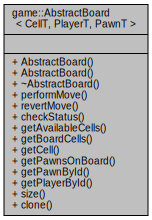
\includegraphics[width=224pt]{classgame_1_1_abstract_board__coll__graph}
\end{center}
\end{figure}
\subsection*{Public Member Functions}
\begin{DoxyCompactItemize}
\item 
\hyperlink{classgame_1_1_abstract_board_a09c49d38999e508f5bc1915209b3cb56}{Abstract\+Board} ()=default
\item 
\hyperlink{classgame_1_1_abstract_board_a648d91d9ffa74ec73fa0844903d9a0fa}{Abstract\+Board} (const \hyperlink{classgame_1_1_abstract_board}{Abstract\+Board}$<$ CellT, PlayerT, PawnT $>$ \&)=delete
\item 
virtual \hyperlink{classgame_1_1_abstract_board_a1331343872024287df1749cea4a96f5e}{$\sim$\+Abstract\+Board} ()
\item 
virtual bool \hyperlink{classgame_1_1_abstract_board_ac2b6d96389ad0ac58d22323d75f91f97}{perform\+Move} (PawnT $\ast$pawn, CellT $\ast$cell)
\begin{DoxyCompactList}\small\item\em perform a movement on the board, sets the current cell on the pawn \end{DoxyCompactList}\item 
virtual const \hyperlink{structgame_1_1_move}{Move}$<$ CellT, PawnT $>$ \hyperlink{classgame_1_1_abstract_board_acc2d5fac68ec019e42fe166b727b7299}{revert\+Move} ()
\begin{DoxyCompactList}\small\item\em revert\+Move \& sets the current cell on the pawn \end{DoxyCompactList}\item 
virtual int \hyperlink{classgame_1_1_abstract_board_a689982e6640633d78008157906c6d63a}{check\+Status} ()=0
\begin{DoxyCompactList}\small\item\em Status of the game. \end{DoxyCompactList}\item 
virtual std\+::vector$<$ CellT $\ast$ $>$ \hyperlink{classgame_1_1_abstract_board_a8def8902ce65947b506ecb129cb7b918}{get\+Available\+Cells} (PawnT $\ast$pawn)=0
\begin{DoxyCompactList}\small\item\em Get the Empty \hyperlink{classgame_1_1_abstract_board_cell}{Abstract\+Board\+Cell} Left. \end{DoxyCompactList}\item 
virtual std\+::vector$<$ CellT $\ast$ $>$ \hyperlink{classgame_1_1_abstract_board_a73d6bef66826688cd6e2bc0f37acb4b0}{get\+Board\+Cells} ()=0
\begin{DoxyCompactList}\small\item\em Get all of the \hyperlink{classgame_1_1_abstract_board_cell}{Abstract\+Board\+Cell}. \end{DoxyCompactList}\item 
virtual CellT $\ast$ \hyperlink{classgame_1_1_abstract_board_af02030d0ae3f44b95fff7c8012e7a066}{get\+Cell} (int line, int col)=0
\begin{DoxyCompactList}\small\item\em Get the Cell. \end{DoxyCompactList}\item 
virtual std\+::vector$<$ PawnT $\ast$ $>$ \hyperlink{classgame_1_1_abstract_board_a9c8a033b23ade01ecce24e95723ffd35}{get\+Pawns\+On\+Board} ()=0
\begin{DoxyCompactList}\small\item\em Get the Players that are presently palying on the board. \end{DoxyCompactList}\item 
virtual PawnT $\ast$ \hyperlink{classgame_1_1_abstract_board_a5d80fa5f0809c746349fc1bab1d8999b}{get\+Pawn\+By\+Id} (const unsigned int id)=0
\begin{DoxyCompactList}\small\item\em Get a player by it\textquotesingle{}s id. \end{DoxyCompactList}\item 
virtual PlayerT $\ast$ \hyperlink{classgame_1_1_abstract_board_a2ae30faf6d02d6d9757020a7ed7932cc}{get\+Player\+By\+Id} (const unsigned int id)=0
\begin{DoxyCompactList}\small\item\em Gets the player corresponding to a certain id. \end{DoxyCompactList}\item 
virtual size\+\_\+t \hyperlink{classgame_1_1_abstract_board_a17bd6905ded76d0005437d288fe8ac21}{size} () const =0
\item 
virtual \hyperlink{classgame_1_1_abstract_board}{Abstract\+Board}$<$ CellT, PlayerT, PawnT $>$ $\ast$ \hyperlink{classgame_1_1_abstract_board_abd467b64fd2c0dfbc0ce87200afb3e9e}{clone} () const =0
\end{DoxyCompactItemize}


\subsection{Detailed Description}
\subsubsection*{template$<$class CellT, class PlayerT, class PawnT$>$\newline
class game\+::\+Abstract\+Board$<$ Cell\+T, Player\+T, Pawn\+T $>$}

Describe the basics of a Board. 


\begin{DoxyTemplParams}{Template Parameters}
{\em CellT} & The type of the cell composing the board \\
\hline
{\em PlayerT} & The type of player linked to the board itself (the player that moves directly on the board)$\ast$ \\
\hline
{\em PawnT} & the type of the pawn playing on the bord \\
\hline
\end{DoxyTemplParams}


\subsection{Constructor \& Destructor Documentation}
\mbox{\Hypertarget{classgame_1_1_abstract_board_a09c49d38999e508f5bc1915209b3cb56}\label{classgame_1_1_abstract_board_a09c49d38999e508f5bc1915209b3cb56}} 
\index{game\+::\+Abstract\+Board@{game\+::\+Abstract\+Board}!Abstract\+Board@{Abstract\+Board}}
\index{Abstract\+Board@{Abstract\+Board}!game\+::\+Abstract\+Board@{game\+::\+Abstract\+Board}}
\subsubsection{\texorpdfstring{Abstract\+Board()}{AbstractBoard()}\hspace{0.1cm}{\footnotesize\ttfamily [1/2]}}
{\footnotesize\ttfamily template$<$class CellT, class PlayerT, class PawnT$>$ \\
\hyperlink{classgame_1_1_abstract_board}{game\+::\+Abstract\+Board}$<$ CellT, PlayerT, PawnT $>$\+::\hyperlink{classgame_1_1_abstract_board}{Abstract\+Board} (\begin{DoxyParamCaption}{ }\end{DoxyParamCaption})\hspace{0.3cm}{\ttfamily [explicit]}, {\ttfamily [default]}}

\mbox{\Hypertarget{classgame_1_1_abstract_board_a648d91d9ffa74ec73fa0844903d9a0fa}\label{classgame_1_1_abstract_board_a648d91d9ffa74ec73fa0844903d9a0fa}} 
\index{game\+::\+Abstract\+Board@{game\+::\+Abstract\+Board}!Abstract\+Board@{Abstract\+Board}}
\index{Abstract\+Board@{Abstract\+Board}!game\+::\+Abstract\+Board@{game\+::\+Abstract\+Board}}
\subsubsection{\texorpdfstring{Abstract\+Board()}{AbstractBoard()}\hspace{0.1cm}{\footnotesize\ttfamily [2/2]}}
{\footnotesize\ttfamily template$<$class CellT, class PlayerT, class PawnT$>$ \\
\hyperlink{classgame_1_1_abstract_board}{game\+::\+Abstract\+Board}$<$ CellT, PlayerT, PawnT $>$\+::\hyperlink{classgame_1_1_abstract_board}{Abstract\+Board} (\begin{DoxyParamCaption}\item[{const \hyperlink{classgame_1_1_abstract_board}{Abstract\+Board}$<$ CellT, PlayerT, PawnT $>$ \&}]{ }\end{DoxyParamCaption})\hspace{0.3cm}{\ttfamily [explicit]}, {\ttfamily [delete]}}

\mbox{\Hypertarget{classgame_1_1_abstract_board_a1331343872024287df1749cea4a96f5e}\label{classgame_1_1_abstract_board_a1331343872024287df1749cea4a96f5e}} 
\index{game\+::\+Abstract\+Board@{game\+::\+Abstract\+Board}!````~Abstract\+Board@{$\sim$\+Abstract\+Board}}
\index{````~Abstract\+Board@{$\sim$\+Abstract\+Board}!game\+::\+Abstract\+Board@{game\+::\+Abstract\+Board}}
\subsubsection{\texorpdfstring{$\sim$\+Abstract\+Board()}{~AbstractBoard()}}
{\footnotesize\ttfamily template$<$class CellT, class PlayerT, class PawnT$>$ \\
virtual \hyperlink{classgame_1_1_abstract_board}{game\+::\+Abstract\+Board}$<$ CellT, PlayerT, PawnT $>$\+::$\sim$\hyperlink{classgame_1_1_abstract_board}{Abstract\+Board} (\begin{DoxyParamCaption}{ }\end{DoxyParamCaption})\hspace{0.3cm}{\ttfamily [inline]}, {\ttfamily [virtual]}}



\subsection{Member Function Documentation}
\mbox{\Hypertarget{classgame_1_1_abstract_board_a689982e6640633d78008157906c6d63a}\label{classgame_1_1_abstract_board_a689982e6640633d78008157906c6d63a}} 
\index{game\+::\+Abstract\+Board@{game\+::\+Abstract\+Board}!check\+Status@{check\+Status}}
\index{check\+Status@{check\+Status}!game\+::\+Abstract\+Board@{game\+::\+Abstract\+Board}}
\subsubsection{\texorpdfstring{check\+Status()}{checkStatus()}}
{\footnotesize\ttfamily template$<$class CellT, class PlayerT, class PawnT$>$ \\
virtual int \hyperlink{classgame_1_1_abstract_board}{game\+::\+Abstract\+Board}$<$ CellT, PlayerT, PawnT $>$\+::check\+Status (\begin{DoxyParamCaption}{ }\end{DoxyParamCaption})\hspace{0.3cm}{\ttfamily [pure virtual]}}



Status of the game. 

\begin{DoxyReturn}{Returns}
game\+\_\+status 
\end{DoxyReturn}


Implemented in \hyperlink{classgame_1_1penguin_1_1_board_a3d659743bc33b43168c82dc4e2d3b00e}{game\+::penguin\+::\+Board}, and \hyperlink{classgame_1_1tic__tac__toe_1_1_board_ae91180193e944c9c58d7d1d0f439918e}{game\+::tic\+\_\+tac\+\_\+toe\+::\+Board}.

Here is the caller graph for this function\+:
\nopagebreak
\begin{figure}[H]
\begin{center}
\leavevmode
\includegraphics[width=350pt]{classgame_1_1_abstract_board_a689982e6640633d78008157906c6d63a_icgraph}
\end{center}
\end{figure}
\mbox{\Hypertarget{classgame_1_1_abstract_board_abd467b64fd2c0dfbc0ce87200afb3e9e}\label{classgame_1_1_abstract_board_abd467b64fd2c0dfbc0ce87200afb3e9e}} 
\index{game\+::\+Abstract\+Board@{game\+::\+Abstract\+Board}!clone@{clone}}
\index{clone@{clone}!game\+::\+Abstract\+Board@{game\+::\+Abstract\+Board}}
\subsubsection{\texorpdfstring{clone()}{clone()}}
{\footnotesize\ttfamily template$<$class CellT, class PlayerT, class PawnT$>$ \\
virtual \hyperlink{classgame_1_1_abstract_board}{Abstract\+Board}$<$CellT, PlayerT, PawnT$>$$\ast$ \hyperlink{classgame_1_1_abstract_board}{game\+::\+Abstract\+Board}$<$ CellT, PlayerT, PawnT $>$\+::clone (\begin{DoxyParamCaption}{ }\end{DoxyParamCaption}) const\hspace{0.3cm}{\ttfamily [pure virtual]}}



Implemented in \hyperlink{classgame_1_1penguin_1_1_board_acad4a3c7bee2103aea4586356ceabb8e}{game\+::penguin\+::\+Board}, and \hyperlink{classgame_1_1tic__tac__toe_1_1_board_a9d7a2c225f06a3410b11b688d9d6bcf8}{game\+::tic\+\_\+tac\+\_\+toe\+::\+Board}.

Here is the caller graph for this function\+:
\nopagebreak
\begin{figure}[H]
\begin{center}
\leavevmode
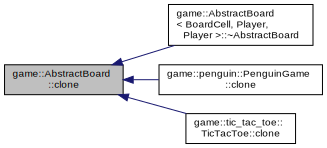
\includegraphics[width=350pt]{classgame_1_1_abstract_board_abd467b64fd2c0dfbc0ce87200afb3e9e_icgraph}
\end{center}
\end{figure}
\mbox{\Hypertarget{classgame_1_1_abstract_board_a8def8902ce65947b506ecb129cb7b918}\label{classgame_1_1_abstract_board_a8def8902ce65947b506ecb129cb7b918}} 
\index{game\+::\+Abstract\+Board@{game\+::\+Abstract\+Board}!get\+Available\+Cells@{get\+Available\+Cells}}
\index{get\+Available\+Cells@{get\+Available\+Cells}!game\+::\+Abstract\+Board@{game\+::\+Abstract\+Board}}
\subsubsection{\texorpdfstring{get\+Available\+Cells()}{getAvailableCells()}}
{\footnotesize\ttfamily template$<$class CellT, class PlayerT, class PawnT$>$ \\
virtual std\+::vector$<$CellT $\ast$$>$ \hyperlink{classgame_1_1_abstract_board}{game\+::\+Abstract\+Board}$<$ CellT, PlayerT, PawnT $>$\+::get\+Available\+Cells (\begin{DoxyParamCaption}\item[{PawnT $\ast$}]{pawn }\end{DoxyParamCaption})\hspace{0.3cm}{\ttfamily [pure virtual]}}



Get the Empty \hyperlink{classgame_1_1_abstract_board_cell}{Abstract\+Board\+Cell} Left. 

\begin{DoxyReturn}{Returns}
std\+::list$<$\+Cell\+T$>$ 
\end{DoxyReturn}
Here is the caller graph for this function\+:
\nopagebreak
\begin{figure}[H]
\begin{center}
\leavevmode
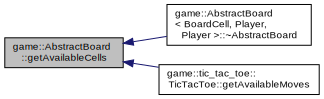
\includegraphics[width=350pt]{classgame_1_1_abstract_board_a8def8902ce65947b506ecb129cb7b918_icgraph}
\end{center}
\end{figure}
\mbox{\Hypertarget{classgame_1_1_abstract_board_a73d6bef66826688cd6e2bc0f37acb4b0}\label{classgame_1_1_abstract_board_a73d6bef66826688cd6e2bc0f37acb4b0}} 
\index{game\+::\+Abstract\+Board@{game\+::\+Abstract\+Board}!get\+Board\+Cells@{get\+Board\+Cells}}
\index{get\+Board\+Cells@{get\+Board\+Cells}!game\+::\+Abstract\+Board@{game\+::\+Abstract\+Board}}
\subsubsection{\texorpdfstring{get\+Board\+Cells()}{getBoardCells()}}
{\footnotesize\ttfamily template$<$class CellT, class PlayerT, class PawnT$>$ \\
virtual std\+::vector$<$CellT $\ast$$>$ \hyperlink{classgame_1_1_abstract_board}{game\+::\+Abstract\+Board}$<$ CellT, PlayerT, PawnT $>$\+::get\+Board\+Cells (\begin{DoxyParamCaption}{ }\end{DoxyParamCaption})\hspace{0.3cm}{\ttfamily [pure virtual]}}



Get all of the \hyperlink{classgame_1_1_abstract_board_cell}{Abstract\+Board\+Cell}. 

\begin{DoxyReturn}{Returns}
std\+::list$<$\+Abstract\+Board\+Cell$>$ 
\end{DoxyReturn}


Implemented in \hyperlink{classgame_1_1penguin_1_1_board_afae3ac9e82200303d28dd4cf7bfa12ec}{game\+::penguin\+::\+Board}, and \hyperlink{classgame_1_1tic__tac__toe_1_1_board_af8bc9dc8a2cfed68aa7d9adead27594e}{game\+::tic\+\_\+tac\+\_\+toe\+::\+Board}.

Here is the caller graph for this function\+:
\nopagebreak
\begin{figure}[H]
\begin{center}
\leavevmode
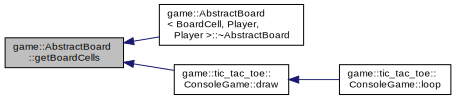
\includegraphics[width=350pt]{classgame_1_1_abstract_board_a73d6bef66826688cd6e2bc0f37acb4b0_icgraph}
\end{center}
\end{figure}
\mbox{\Hypertarget{classgame_1_1_abstract_board_af02030d0ae3f44b95fff7c8012e7a066}\label{classgame_1_1_abstract_board_af02030d0ae3f44b95fff7c8012e7a066}} 
\index{game\+::\+Abstract\+Board@{game\+::\+Abstract\+Board}!get\+Cell@{get\+Cell}}
\index{get\+Cell@{get\+Cell}!game\+::\+Abstract\+Board@{game\+::\+Abstract\+Board}}
\subsubsection{\texorpdfstring{get\+Cell()}{getCell()}}
{\footnotesize\ttfamily template$<$class CellT, class PlayerT, class PawnT$>$ \\
virtual CellT$\ast$ \hyperlink{classgame_1_1_abstract_board}{game\+::\+Abstract\+Board}$<$ CellT, PlayerT, PawnT $>$\+::get\+Cell (\begin{DoxyParamCaption}\item[{int}]{line,  }\item[{int}]{col }\end{DoxyParamCaption})\hspace{0.3cm}{\ttfamily [pure virtual]}}



Get the Cell. 


\begin{DoxyParams}{Parameters}
{\em line} & line coord \\
\hline
{\em col} & col coord \\
\hline
\end{DoxyParams}
\begin{DoxyReturn}{Returns}
the targeted cell 
\end{DoxyReturn}


Implemented in \hyperlink{classgame_1_1penguin_1_1_board_ac9fbe04a302208fcb5f66e717182b6d4}{game\+::penguin\+::\+Board}, and \hyperlink{classgame_1_1tic__tac__toe_1_1_board_ab5c00479b4dabd60bef9ea00fce23779}{game\+::tic\+\_\+tac\+\_\+toe\+::\+Board}.

Here is the caller graph for this function\+:
\nopagebreak
\begin{figure}[H]
\begin{center}
\leavevmode
\includegraphics[width=350pt]{classgame_1_1_abstract_board_af02030d0ae3f44b95fff7c8012e7a066_icgraph}
\end{center}
\end{figure}
\mbox{\Hypertarget{classgame_1_1_abstract_board_a5d80fa5f0809c746349fc1bab1d8999b}\label{classgame_1_1_abstract_board_a5d80fa5f0809c746349fc1bab1d8999b}} 
\index{game\+::\+Abstract\+Board@{game\+::\+Abstract\+Board}!get\+Pawn\+By\+Id@{get\+Pawn\+By\+Id}}
\index{get\+Pawn\+By\+Id@{get\+Pawn\+By\+Id}!game\+::\+Abstract\+Board@{game\+::\+Abstract\+Board}}
\subsubsection{\texorpdfstring{get\+Pawn\+By\+Id()}{getPawnById()}}
{\footnotesize\ttfamily template$<$class CellT, class PlayerT, class PawnT$>$ \\
virtual PawnT$\ast$ \hyperlink{classgame_1_1_abstract_board}{game\+::\+Abstract\+Board}$<$ CellT, PlayerT, PawnT $>$\+::get\+Pawn\+By\+Id (\begin{DoxyParamCaption}\item[{const unsigned int}]{id }\end{DoxyParamCaption})\hspace{0.3cm}{\ttfamily [pure virtual]}}



Get a player by it\textquotesingle{}s id. 


\begin{DoxyParams}{Parameters}
{\em id} & the id of the player wanted \\
\hline
\end{DoxyParams}
\begin{DoxyReturn}{Returns}
Pawn\+T$\ast$ the pawn wanted, or null if it doesn\textquotesingle{}t exists 
\end{DoxyReturn}


Implemented in \hyperlink{classgame_1_1penguin_1_1_board_acae84c13dacef3bd988d1ea9a41d055f}{game\+::penguin\+::\+Board}, and \hyperlink{classgame_1_1tic__tac__toe_1_1_board_a7f11ea8d48d9613057dd8164a7610f9a}{game\+::tic\+\_\+tac\+\_\+toe\+::\+Board}.

Here is the caller graph for this function\+:
\nopagebreak
\begin{figure}[H]
\begin{center}
\leavevmode
\includegraphics[width=350pt]{classgame_1_1_abstract_board_a5d80fa5f0809c746349fc1bab1d8999b_icgraph}
\end{center}
\end{figure}
\mbox{\Hypertarget{classgame_1_1_abstract_board_a9c8a033b23ade01ecce24e95723ffd35}\label{classgame_1_1_abstract_board_a9c8a033b23ade01ecce24e95723ffd35}} 
\index{game\+::\+Abstract\+Board@{game\+::\+Abstract\+Board}!get\+Pawns\+On\+Board@{get\+Pawns\+On\+Board}}
\index{get\+Pawns\+On\+Board@{get\+Pawns\+On\+Board}!game\+::\+Abstract\+Board@{game\+::\+Abstract\+Board}}
\subsubsection{\texorpdfstring{get\+Pawns\+On\+Board()}{getPawnsOnBoard()}}
{\footnotesize\ttfamily template$<$class CellT, class PlayerT, class PawnT$>$ \\
virtual std\+::vector$<$PawnT $\ast$$>$ \hyperlink{classgame_1_1_abstract_board}{game\+::\+Abstract\+Board}$<$ CellT, PlayerT, PawnT $>$\+::get\+Pawns\+On\+Board (\begin{DoxyParamCaption}{ }\end{DoxyParamCaption})\hspace{0.3cm}{\ttfamily [pure virtual]}}



Get the Players that are presently palying on the board. 

\begin{DoxyReturn}{Returns}
std\+::vector$<$\+Player\+T $\ast$$>$ a vector of the players 
\end{DoxyReturn}


Implemented in \hyperlink{classgame_1_1penguin_1_1_board_a13a38d7c935dd363d7ec9394488539ee}{game\+::penguin\+::\+Board}, and \hyperlink{classgame_1_1tic__tac__toe_1_1_board_a84cb90a6d844d80ecd5857fb4dc9ad1a}{game\+::tic\+\_\+tac\+\_\+toe\+::\+Board}.

Here is the caller graph for this function\+:
\nopagebreak
\begin{figure}[H]
\begin{center}
\leavevmode
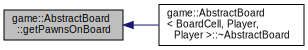
\includegraphics[width=350pt]{classgame_1_1_abstract_board_a9c8a033b23ade01ecce24e95723ffd35_icgraph}
\end{center}
\end{figure}
\mbox{\Hypertarget{classgame_1_1_abstract_board_a2ae30faf6d02d6d9757020a7ed7932cc}\label{classgame_1_1_abstract_board_a2ae30faf6d02d6d9757020a7ed7932cc}} 
\index{game\+::\+Abstract\+Board@{game\+::\+Abstract\+Board}!get\+Player\+By\+Id@{get\+Player\+By\+Id}}
\index{get\+Player\+By\+Id@{get\+Player\+By\+Id}!game\+::\+Abstract\+Board@{game\+::\+Abstract\+Board}}
\subsubsection{\texorpdfstring{get\+Player\+By\+Id()}{getPlayerById()}}
{\footnotesize\ttfamily template$<$class CellT, class PlayerT, class PawnT$>$ \\
virtual PlayerT$\ast$ \hyperlink{classgame_1_1_abstract_board}{game\+::\+Abstract\+Board}$<$ CellT, PlayerT, PawnT $>$\+::get\+Player\+By\+Id (\begin{DoxyParamCaption}\item[{const unsigned int}]{id }\end{DoxyParamCaption})\hspace{0.3cm}{\ttfamily [pure virtual]}}



Gets the player corresponding to a certain id. 


\begin{DoxyParams}{Parameters}
{\em id} & the id of the player \\
\hline
\end{DoxyParams}
\begin{DoxyReturn}{Returns}
Player\+T$\ast$ the player wanted 
\end{DoxyReturn}


Implemented in \hyperlink{classgame_1_1penguin_1_1_board_a8728b4381bc2e007710d275bb226cf95}{game\+::penguin\+::\+Board}, and \hyperlink{classgame_1_1tic__tac__toe_1_1_board_a7907b8fc363b7e33d585edbc7ec102ae}{game\+::tic\+\_\+tac\+\_\+toe\+::\+Board}.

Here is the caller graph for this function\+:
\nopagebreak
\begin{figure}[H]
\begin{center}
\leavevmode
\includegraphics[width=350pt]{classgame_1_1_abstract_board_a2ae30faf6d02d6d9757020a7ed7932cc_icgraph}
\end{center}
\end{figure}
\mbox{\Hypertarget{classgame_1_1_abstract_board_ac2b6d96389ad0ac58d22323d75f91f97}\label{classgame_1_1_abstract_board_ac2b6d96389ad0ac58d22323d75f91f97}} 
\index{game\+::\+Abstract\+Board@{game\+::\+Abstract\+Board}!perform\+Move@{perform\+Move}}
\index{perform\+Move@{perform\+Move}!game\+::\+Abstract\+Board@{game\+::\+Abstract\+Board}}
\subsubsection{\texorpdfstring{perform\+Move()}{performMove()}}
{\footnotesize\ttfamily template$<$class CellT, class PlayerT , class PawnT$>$ \\
bool \hyperlink{classgame_1_1_abstract_board}{game\+::\+Abstract\+Board}$<$ CellT, PlayerT, PawnT $>$\+::perform\+Move (\begin{DoxyParamCaption}\item[{PawnT $\ast$}]{pawn,  }\item[{CellT $\ast$}]{cell }\end{DoxyParamCaption})\hspace{0.3cm}{\ttfamily [virtual]}}



perform a movement on the board, sets the current cell on the pawn 


\begin{DoxyParams}{Parameters}
{\em player} & the player that realizes the movement \\
\hline
{\em cell} & the cell targeted\\
\hline
\end{DoxyParams}
\begin{DoxyReturn}{Returns}
true if the move is allowed, false otherwise 
\end{DoxyReturn}
Here is the caller graph for this function\+:
\nopagebreak
\begin{figure}[H]
\begin{center}
\leavevmode
\includegraphics[width=350pt]{classgame_1_1_abstract_board_ac2b6d96389ad0ac58d22323d75f91f97_icgraph}
\end{center}
\end{figure}
\mbox{\Hypertarget{classgame_1_1_abstract_board_acc2d5fac68ec019e42fe166b727b7299}\label{classgame_1_1_abstract_board_acc2d5fac68ec019e42fe166b727b7299}} 
\index{game\+::\+Abstract\+Board@{game\+::\+Abstract\+Board}!revert\+Move@{revert\+Move}}
\index{revert\+Move@{revert\+Move}!game\+::\+Abstract\+Board@{game\+::\+Abstract\+Board}}
\subsubsection{\texorpdfstring{revert\+Move()}{revertMove()}}
{\footnotesize\ttfamily template$<$class CellT , class PlayerT , class PawnT $>$ \\
const \hyperlink{structgame_1_1_move}{Move}$<$ CellT, PawnT $>$ \hyperlink{classgame_1_1_abstract_board}{game\+::\+Abstract\+Board}$<$ CellT, PlayerT, PawnT $>$\+::revert\+Move (\begin{DoxyParamCaption}{ }\end{DoxyParamCaption})\hspace{0.3cm}{\ttfamily [virtual]}}



revert\+Move \& sets the current cell on the pawn 

\begin{DoxyReturn}{Returns}
const Move$<$\+Cell\+T, Pawn\+T$>$ 
\end{DoxyReturn}


Reimplemented in \hyperlink{classgame_1_1penguin_1_1_board_a45ecb5bba50b4d03592ac4ddf9255b49}{game\+::penguin\+::\+Board}, and \hyperlink{classgame_1_1tic__tac__toe_1_1_board_ac77aad0bb0945d12a959bb8db0e31908}{game\+::tic\+\_\+tac\+\_\+toe\+::\+Board}.

Here is the caller graph for this function\+:
\nopagebreak
\begin{figure}[H]
\begin{center}
\leavevmode
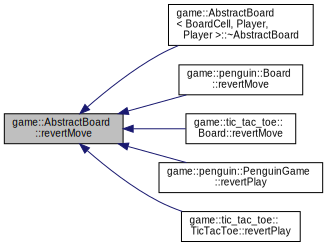
\includegraphics[width=350pt]{classgame_1_1_abstract_board_acc2d5fac68ec019e42fe166b727b7299_icgraph}
\end{center}
\end{figure}
\mbox{\Hypertarget{classgame_1_1_abstract_board_a17bd6905ded76d0005437d288fe8ac21}\label{classgame_1_1_abstract_board_a17bd6905ded76d0005437d288fe8ac21}} 
\index{game\+::\+Abstract\+Board@{game\+::\+Abstract\+Board}!size@{size}}
\index{size@{size}!game\+::\+Abstract\+Board@{game\+::\+Abstract\+Board}}
\subsubsection{\texorpdfstring{size()}{size()}}
{\footnotesize\ttfamily template$<$class CellT, class PlayerT, class PawnT$>$ \\
virtual size\+\_\+t \hyperlink{classgame_1_1_abstract_board}{game\+::\+Abstract\+Board}$<$ CellT, PlayerT, PawnT $>$\+::size (\begin{DoxyParamCaption}{ }\end{DoxyParamCaption}) const\hspace{0.3cm}{\ttfamily [pure virtual]}}



Implemented in \hyperlink{classgame_1_1penguin_1_1_board_a7636e3bdb2da72d2a6395b1a2d846394}{game\+::penguin\+::\+Board}, and \hyperlink{classgame_1_1tic__tac__toe_1_1_board_ac9d2d5da2263bb6166f93eec382380db}{game\+::tic\+\_\+tac\+\_\+toe\+::\+Board}.

Here is the caller graph for this function\+:
\nopagebreak
\begin{figure}[H]
\begin{center}
\leavevmode
\includegraphics[width=350pt]{classgame_1_1_abstract_board_a17bd6905ded76d0005437d288fe8ac21_icgraph}
\end{center}
\end{figure}


The documentation for this class was generated from the following files\+:\begin{DoxyCompactItemize}
\item 
/workspace/src/game\+\_\+logic/\hyperlink{_abstract_board_8hpp}{Abstract\+Board.\+hpp}\item 
/workspace/src/game\+\_\+logic/\hyperlink{_abstract_board_8cpp}{Abstract\+Board.\+cpp}\end{DoxyCompactItemize}

\hypertarget{classgame_1_1_abstract_board_cell}{}\section{game\+:\+:Abstract\+Board\+Cell Class Reference}
\label{classgame_1_1_abstract_board_cell}\index{game\+::\+Abstract\+Board\+Cell@{game\+::\+Abstract\+Board\+Cell}}


{\ttfamily \#include $<$Abstract\+Board\+Cell.\+hpp$>$}



Inheritance diagram for game\+:\+:Abstract\+Board\+Cell\+:
\nopagebreak
\begin{figure}[H]
\begin{center}
\leavevmode
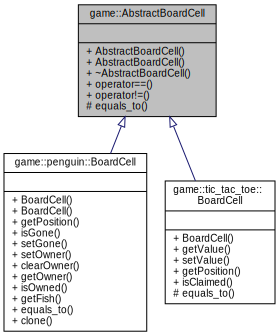
\includegraphics[width=350pt]{classgame_1_1_abstract_board_cell__inherit__graph}
\end{center}
\end{figure}


Collaboration diagram for game\+:\+:Abstract\+Board\+Cell\+:
\nopagebreak
\begin{figure}[H]
\begin{center}
\leavevmode
\includegraphics[width=218pt]{classgame_1_1_abstract_board_cell__coll__graph}
\end{center}
\end{figure}
\subsection*{Public Member Functions}
\begin{DoxyCompactItemize}
\item 
\hyperlink{classgame_1_1_abstract_board_cell_a7270efe993a1dfeafc93b41b21590b18}{Abstract\+Board\+Cell} ()=default
\item 
\hyperlink{classgame_1_1_abstract_board_cell_ae4e615cb466fa0ce4fa028c8f840e065}{Abstract\+Board\+Cell} (const \hyperlink{classgame_1_1_abstract_board_cell}{Abstract\+Board\+Cell} \&)=default
\item 
virtual \hyperlink{classgame_1_1_abstract_board_cell_a5b1ce48a00a25ad6485af754f3c57b66}{$\sim$\+Abstract\+Board\+Cell} ()
\item 
bool \hyperlink{classgame_1_1_abstract_board_cell_ad2e86ef567d46428275e9eb4372d788f}{operator==} (const \hyperlink{classgame_1_1_abstract_board_cell}{Abstract\+Board\+Cell} \&cell)
\item 
bool \hyperlink{classgame_1_1_abstract_board_cell_a4a649f51a349dad0246fed9e8faee922}{operator!=} (const \hyperlink{classgame_1_1_abstract_board_cell}{Abstract\+Board\+Cell} \&cell)
\end{DoxyCompactItemize}
\subsection*{Protected Member Functions}
\begin{DoxyCompactItemize}
\item 
virtual bool \hyperlink{classgame_1_1_abstract_board_cell_a3939330bed75f3a408af228e86ec93af}{equals\+\_\+to} (const \hyperlink{classgame_1_1_abstract_board_cell}{Abstract\+Board\+Cell} \&cell) const =0
\end{DoxyCompactItemize}


\subsection{Constructor \& Destructor Documentation}
\mbox{\Hypertarget{classgame_1_1_abstract_board_cell_a7270efe993a1dfeafc93b41b21590b18}\label{classgame_1_1_abstract_board_cell_a7270efe993a1dfeafc93b41b21590b18}} 
\index{game\+::\+Abstract\+Board\+Cell@{game\+::\+Abstract\+Board\+Cell}!Abstract\+Board\+Cell@{Abstract\+Board\+Cell}}
\index{Abstract\+Board\+Cell@{Abstract\+Board\+Cell}!game\+::\+Abstract\+Board\+Cell@{game\+::\+Abstract\+Board\+Cell}}
\subsubsection{\texorpdfstring{Abstract\+Board\+Cell()}{AbstractBoardCell()}\hspace{0.1cm}{\footnotesize\ttfamily [1/2]}}
{\footnotesize\ttfamily game\+::\+Abstract\+Board\+Cell\+::\+Abstract\+Board\+Cell (\begin{DoxyParamCaption}{ }\end{DoxyParamCaption})\hspace{0.3cm}{\ttfamily [explicit]}, {\ttfamily [default]}}

\mbox{\Hypertarget{classgame_1_1_abstract_board_cell_ae4e615cb466fa0ce4fa028c8f840e065}\label{classgame_1_1_abstract_board_cell_ae4e615cb466fa0ce4fa028c8f840e065}} 
\index{game\+::\+Abstract\+Board\+Cell@{game\+::\+Abstract\+Board\+Cell}!Abstract\+Board\+Cell@{Abstract\+Board\+Cell}}
\index{Abstract\+Board\+Cell@{Abstract\+Board\+Cell}!game\+::\+Abstract\+Board\+Cell@{game\+::\+Abstract\+Board\+Cell}}
\subsubsection{\texorpdfstring{Abstract\+Board\+Cell()}{AbstractBoardCell()}\hspace{0.1cm}{\footnotesize\ttfamily [2/2]}}
{\footnotesize\ttfamily game\+::\+Abstract\+Board\+Cell\+::\+Abstract\+Board\+Cell (\begin{DoxyParamCaption}\item[{const \hyperlink{classgame_1_1_abstract_board_cell}{Abstract\+Board\+Cell} \&}]{ }\end{DoxyParamCaption})\hspace{0.3cm}{\ttfamily [explicit]}, {\ttfamily [default]}}

\mbox{\Hypertarget{classgame_1_1_abstract_board_cell_a5b1ce48a00a25ad6485af754f3c57b66}\label{classgame_1_1_abstract_board_cell_a5b1ce48a00a25ad6485af754f3c57b66}} 
\index{game\+::\+Abstract\+Board\+Cell@{game\+::\+Abstract\+Board\+Cell}!````~Abstract\+Board\+Cell@{$\sim$\+Abstract\+Board\+Cell}}
\index{````~Abstract\+Board\+Cell@{$\sim$\+Abstract\+Board\+Cell}!game\+::\+Abstract\+Board\+Cell@{game\+::\+Abstract\+Board\+Cell}}
\subsubsection{\texorpdfstring{$\sim$\+Abstract\+Board\+Cell()}{~AbstractBoardCell()}}
{\footnotesize\ttfamily virtual game\+::\+Abstract\+Board\+Cell\+::$\sim$\+Abstract\+Board\+Cell (\begin{DoxyParamCaption}{ }\end{DoxyParamCaption})\hspace{0.3cm}{\ttfamily [inline]}, {\ttfamily [virtual]}}



\subsection{Member Function Documentation}
\mbox{\Hypertarget{classgame_1_1_abstract_board_cell_a3939330bed75f3a408af228e86ec93af}\label{classgame_1_1_abstract_board_cell_a3939330bed75f3a408af228e86ec93af}} 
\index{game\+::\+Abstract\+Board\+Cell@{game\+::\+Abstract\+Board\+Cell}!equals\+\_\+to@{equals\+\_\+to}}
\index{equals\+\_\+to@{equals\+\_\+to}!game\+::\+Abstract\+Board\+Cell@{game\+::\+Abstract\+Board\+Cell}}
\subsubsection{\texorpdfstring{equals\+\_\+to()}{equals\_to()}}
{\footnotesize\ttfamily virtual bool game\+::\+Abstract\+Board\+Cell\+::equals\+\_\+to (\begin{DoxyParamCaption}\item[{const \hyperlink{classgame_1_1_abstract_board_cell}{Abstract\+Board\+Cell} \&}]{cell }\end{DoxyParamCaption}) const\hspace{0.3cm}{\ttfamily [protected]}, {\ttfamily [pure virtual]}}



Implemented in \hyperlink{classgame_1_1penguin_1_1_board_cell_a1ed5a3134f831bef111c6294c07388bf}{game\+::penguin\+::\+Board\+Cell}, and \hyperlink{classgame_1_1tic__tac__toe_1_1_board_cell_a909bb91d32553cebbe9749bd6814b8f4}{game\+::tic\+\_\+tac\+\_\+toe\+::\+Board\+Cell}.

Here is the caller graph for this function\+:
\nopagebreak
\begin{figure}[H]
\begin{center}
\leavevmode
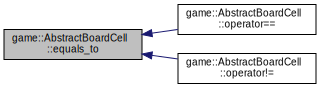
\includegraphics[width=350pt]{classgame_1_1_abstract_board_cell_a3939330bed75f3a408af228e86ec93af_icgraph}
\end{center}
\end{figure}
\mbox{\Hypertarget{classgame_1_1_abstract_board_cell_a4a649f51a349dad0246fed9e8faee922}\label{classgame_1_1_abstract_board_cell_a4a649f51a349dad0246fed9e8faee922}} 
\index{game\+::\+Abstract\+Board\+Cell@{game\+::\+Abstract\+Board\+Cell}!operator"!=@{operator"!=}}
\index{operator"!=@{operator"!=}!game\+::\+Abstract\+Board\+Cell@{game\+::\+Abstract\+Board\+Cell}}
\subsubsection{\texorpdfstring{operator"!=()}{operator!=()}}
{\footnotesize\ttfamily bool game\+::\+Abstract\+Board\+Cell\+::operator!= (\begin{DoxyParamCaption}\item[{const \hyperlink{classgame_1_1_abstract_board_cell}{Abstract\+Board\+Cell} \&}]{cell }\end{DoxyParamCaption})\hspace{0.3cm}{\ttfamily [inline]}}

Here is the call graph for this function\+:
\nopagebreak
\begin{figure}[H]
\begin{center}
\leavevmode
\includegraphics[width=350pt]{classgame_1_1_abstract_board_cell_a4a649f51a349dad0246fed9e8faee922_cgraph}
\end{center}
\end{figure}
\mbox{\Hypertarget{classgame_1_1_abstract_board_cell_ad2e86ef567d46428275e9eb4372d788f}\label{classgame_1_1_abstract_board_cell_ad2e86ef567d46428275e9eb4372d788f}} 
\index{game\+::\+Abstract\+Board\+Cell@{game\+::\+Abstract\+Board\+Cell}!operator==@{operator==}}
\index{operator==@{operator==}!game\+::\+Abstract\+Board\+Cell@{game\+::\+Abstract\+Board\+Cell}}
\subsubsection{\texorpdfstring{operator==()}{operator==()}}
{\footnotesize\ttfamily bool game\+::\+Abstract\+Board\+Cell\+::operator== (\begin{DoxyParamCaption}\item[{const \hyperlink{classgame_1_1_abstract_board_cell}{Abstract\+Board\+Cell} \&}]{cell }\end{DoxyParamCaption})\hspace{0.3cm}{\ttfamily [inline]}}

Here is the call graph for this function\+:
\nopagebreak
\begin{figure}[H]
\begin{center}
\leavevmode
\includegraphics[width=350pt]{classgame_1_1_abstract_board_cell_ad2e86ef567d46428275e9eb4372d788f_cgraph}
\end{center}
\end{figure}


The documentation for this class was generated from the following file\+:\begin{DoxyCompactItemize}
\item 
/workspace/src/game\+\_\+logic/\hyperlink{_abstract_board_cell_8hpp}{Abstract\+Board\+Cell.\+hpp}\end{DoxyCompactItemize}

\hypertarget{classgame_1_1_abstract_game}{}\section{game\+:\+:Abstract\+Game$<$ CellT, PlayerT, PawnT $>$ Class Template Reference}
\label{classgame_1_1_abstract_game}\index{game\+::\+Abstract\+Game$<$ Cell\+T, Player\+T, Pawn\+T $>$@{game\+::\+Abstract\+Game$<$ Cell\+T, Player\+T, Pawn\+T $>$}}


{\ttfamily \#include $<$Abstract\+Game.\+hpp$>$}



Inheritance diagram for game\+:\+:Abstract\+Game$<$ CellT, PlayerT, PawnT $>$\+:
\nopagebreak
\begin{figure}[H]
\begin{center}
\leavevmode
\includegraphics[height=550pt]{classgame_1_1_abstract_game__inherit__graph}
\end{center}
\end{figure}


Collaboration diagram for game\+:\+:Abstract\+Game$<$ CellT, PlayerT, PawnT $>$\+:
\nopagebreak
\begin{figure}[H]
\begin{center}
\leavevmode
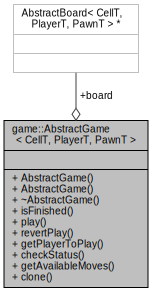
\includegraphics[width=224pt]{classgame_1_1_abstract_game__coll__graph}
\end{center}
\end{figure}
\subsection*{Public Member Functions}
\begin{DoxyCompactItemize}
\item 
\hyperlink{classgame_1_1_abstract_game_ae01d0d7523f6958450a404e6aafa5cd0}{Abstract\+Game} (\hyperlink{classgame_1_1_abstract_board}{Abstract\+Board}$<$ CellT, PlayerT, PawnT $>$ $\ast$\hyperlink{classgame_1_1_abstract_game_a6df5f611daa1731c4c8d3d5e6289e7e5}{board})
\item 
\hyperlink{classgame_1_1_abstract_game_a4947b8268696a1d6d2d15bfad1cbe197}{Abstract\+Game} (const \hyperlink{classgame_1_1_abstract_game}{Abstract\+Game}$<$ CellT, PlayerT, PawnT $>$ \&)=default
\item 
virtual \hyperlink{classgame_1_1_abstract_game_aadcf523d247e4f8beccc539a08f40464}{$\sim$\+Abstract\+Game} ()
\item 
virtual bool \hyperlink{classgame_1_1_abstract_game_a598679eebf40ccc300e9065bce875fd1}{is\+Finished} () const =0
\begin{DoxyCompactList}\small\item\em Tells if the game is finished yet. \end{DoxyCompactList}\item 
virtual bool \hyperlink{classgame_1_1_abstract_game_a5eb974a047c5179c28cf77ec60d77cdc}{play} (PawnT $\ast$pawn, CellT $\ast$cell)=0
\begin{DoxyCompactList}\small\item\em play one round of the game \end{DoxyCompactList}\item 
virtual const \hyperlink{structgame_1_1_move}{Move}$<$ CellT, PawnT $>$ \hyperlink{classgame_1_1_abstract_game_af6088ae12ed47989dde7f8869e79d934}{revert\+Play} ()=0
\item 
virtual unsigned int \hyperlink{classgame_1_1_abstract_game_a059d72564d4658be3c246d8865080d92}{get\+Player\+To\+Play} ()=0
\begin{DoxyCompactList}\small\item\em Get the player who hadn\textquotesingle{}t play yet. \end{DoxyCompactList}\item 
virtual int \hyperlink{classgame_1_1_abstract_game_a3683d4f37908f769a470af6ebf73d849}{check\+Status} () const =0
\begin{DoxyCompactList}\small\item\em Checks the status of the game, if won, draw. \end{DoxyCompactList}\item 
virtual std\+::vector$<$ \hyperlink{structgame_1_1_move}{Move}$<$ CellT, PawnT $>$ $>$ \hyperlink{classgame_1_1_abstract_game_a01bbff0af90cc978203726bc7f914a7b}{get\+Available\+Moves} (PlayerT $\ast$player)=0
\begin{DoxyCompactList}\small\item\em Get the available moves to a player. \end{DoxyCompactList}\item 
virtual \hyperlink{classgame_1_1_abstract_game}{Abstract\+Game}$<$ CellT, PlayerT, PawnT $>$ $\ast$ \hyperlink{classgame_1_1_abstract_game_a226baac1f32a8f6672d922675ffddbf6}{clone} () const =0
\begin{DoxyCompactList}\small\item\em Clone function for clonning games. \end{DoxyCompactList}\end{DoxyCompactItemize}
\subsection*{Public Attributes}
\begin{DoxyCompactItemize}
\item 
\hyperlink{classgame_1_1_abstract_board}{Abstract\+Board}$<$ CellT, PlayerT, PawnT $>$ $\ast$ \hyperlink{classgame_1_1_abstract_game_a6df5f611daa1731c4c8d3d5e6289e7e5}{board}
\end{DoxyCompactItemize}


\subsection{Constructor \& Destructor Documentation}
\mbox{\Hypertarget{classgame_1_1_abstract_game_ae01d0d7523f6958450a404e6aafa5cd0}\label{classgame_1_1_abstract_game_ae01d0d7523f6958450a404e6aafa5cd0}} 
\index{game\+::\+Abstract\+Game@{game\+::\+Abstract\+Game}!Abstract\+Game@{Abstract\+Game}}
\index{Abstract\+Game@{Abstract\+Game}!game\+::\+Abstract\+Game@{game\+::\+Abstract\+Game}}
\subsubsection{\texorpdfstring{Abstract\+Game()}{AbstractGame()}\hspace{0.1cm}{\footnotesize\ttfamily [1/2]}}
{\footnotesize\ttfamily template$<$class CellT, class PlayerT, class PawnT$>$ \\
\hyperlink{classgame_1_1_abstract_game}{game\+::\+Abstract\+Game}$<$ CellT, PlayerT, PawnT $>$\+::\hyperlink{classgame_1_1_abstract_game}{Abstract\+Game} (\begin{DoxyParamCaption}\item[{\hyperlink{classgame_1_1_abstract_board}{Abstract\+Board}$<$ CellT, PlayerT, PawnT $>$ $\ast$}]{board }\end{DoxyParamCaption})\hspace{0.3cm}{\ttfamily [explicit]}}

\mbox{\Hypertarget{classgame_1_1_abstract_game_a4947b8268696a1d6d2d15bfad1cbe197}\label{classgame_1_1_abstract_game_a4947b8268696a1d6d2d15bfad1cbe197}} 
\index{game\+::\+Abstract\+Game@{game\+::\+Abstract\+Game}!Abstract\+Game@{Abstract\+Game}}
\index{Abstract\+Game@{Abstract\+Game}!game\+::\+Abstract\+Game@{game\+::\+Abstract\+Game}}
\subsubsection{\texorpdfstring{Abstract\+Game()}{AbstractGame()}\hspace{0.1cm}{\footnotesize\ttfamily [2/2]}}
{\footnotesize\ttfamily template$<$class CellT, class PlayerT, class PawnT$>$ \\
\hyperlink{classgame_1_1_abstract_game}{game\+::\+Abstract\+Game}$<$ CellT, PlayerT, PawnT $>$\+::\hyperlink{classgame_1_1_abstract_game}{Abstract\+Game} (\begin{DoxyParamCaption}\item[{const \hyperlink{classgame_1_1_abstract_game}{Abstract\+Game}$<$ CellT, PlayerT, PawnT $>$ \&}]{ }\end{DoxyParamCaption})\hspace{0.3cm}{\ttfamily [explicit]}, {\ttfamily [default]}}

\mbox{\Hypertarget{classgame_1_1_abstract_game_aadcf523d247e4f8beccc539a08f40464}\label{classgame_1_1_abstract_game_aadcf523d247e4f8beccc539a08f40464}} 
\index{game\+::\+Abstract\+Game@{game\+::\+Abstract\+Game}!````~Abstract\+Game@{$\sim$\+Abstract\+Game}}
\index{````~Abstract\+Game@{$\sim$\+Abstract\+Game}!game\+::\+Abstract\+Game@{game\+::\+Abstract\+Game}}
\subsubsection{\texorpdfstring{$\sim$\+Abstract\+Game()}{~AbstractGame()}}
{\footnotesize\ttfamily template$<$class CellT, class PlayerT, class PawnT$>$ \\
virtual \hyperlink{classgame_1_1_abstract_game}{game\+::\+Abstract\+Game}$<$ CellT, PlayerT, PawnT $>$\+::$\sim$\hyperlink{classgame_1_1_abstract_game}{Abstract\+Game} (\begin{DoxyParamCaption}{ }\end{DoxyParamCaption})\hspace{0.3cm}{\ttfamily [inline]}, {\ttfamily [virtual]}}



\subsection{Member Function Documentation}
\mbox{\Hypertarget{classgame_1_1_abstract_game_a3683d4f37908f769a470af6ebf73d849}\label{classgame_1_1_abstract_game_a3683d4f37908f769a470af6ebf73d849}} 
\index{game\+::\+Abstract\+Game@{game\+::\+Abstract\+Game}!check\+Status@{check\+Status}}
\index{check\+Status@{check\+Status}!game\+::\+Abstract\+Game@{game\+::\+Abstract\+Game}}
\subsubsection{\texorpdfstring{check\+Status()}{checkStatus()}}
{\footnotesize\ttfamily template$<$class CellT, class PlayerT, class PawnT$>$ \\
virtual int \hyperlink{classgame_1_1_abstract_game}{game\+::\+Abstract\+Game}$<$ CellT, PlayerT, PawnT $>$\+::check\+Status (\begin{DoxyParamCaption}{ }\end{DoxyParamCaption}) const\hspace{0.3cm}{\ttfamily [pure virtual]}}



Checks the status of the game, if won, draw. 

\begin{DoxyReturn}{Returns}
int when won \+: the id of the winner, -\/1 if draw, 0 otherwise 
\end{DoxyReturn}


Implemented in \hyperlink{classgame_1_1penguin_1_1_penguin_game_af255dc5b05ef5244ac864d4aa2d3be2e}{game\+::penguin\+::\+Penguin\+Game}, and \hyperlink{classgame_1_1tic__tac__toe_1_1_tic_tac_toe_a033d73237ae31a39c23a0e887adbce2f}{game\+::tic\+\_\+tac\+\_\+toe\+::\+Tic\+Tac\+Toe}.

Here is the caller graph for this function\+:
\nopagebreak
\begin{figure}[H]
\begin{center}
\leavevmode
\includegraphics[width=350pt]{classgame_1_1_abstract_game_a3683d4f37908f769a470af6ebf73d849_icgraph}
\end{center}
\end{figure}
\mbox{\Hypertarget{classgame_1_1_abstract_game_a226baac1f32a8f6672d922675ffddbf6}\label{classgame_1_1_abstract_game_a226baac1f32a8f6672d922675ffddbf6}} 
\index{game\+::\+Abstract\+Game@{game\+::\+Abstract\+Game}!clone@{clone}}
\index{clone@{clone}!game\+::\+Abstract\+Game@{game\+::\+Abstract\+Game}}
\subsubsection{\texorpdfstring{clone()}{clone()}}
{\footnotesize\ttfamily template$<$class CellT, class PlayerT, class PawnT$>$ \\
virtual \hyperlink{classgame_1_1_abstract_game}{Abstract\+Game}$<$CellT, PlayerT, PawnT$>$$\ast$ \hyperlink{classgame_1_1_abstract_game}{game\+::\+Abstract\+Game}$<$ CellT, PlayerT, PawnT $>$\+::clone (\begin{DoxyParamCaption}{ }\end{DoxyParamCaption}) const\hspace{0.3cm}{\ttfamily [pure virtual]}}



Clone function for clonning games. 

\begin{DoxyReturn}{Returns}
Abstract\+Game$\ast$ 
\end{DoxyReturn}


Implemented in \hyperlink{classgame_1_1penguin_1_1_penguin_game_af4277cfe44814a9b99051348f25ce264}{game\+::penguin\+::\+Penguin\+Game}, and \hyperlink{classgame_1_1tic__tac__toe_1_1_tic_tac_toe_a11f31f44ee9ebe8c394bcc9f2a74fab4}{game\+::tic\+\_\+tac\+\_\+toe\+::\+Tic\+Tac\+Toe}.

Here is the caller graph for this function\+:
\nopagebreak
\begin{figure}[H]
\begin{center}
\leavevmode
\includegraphics[width=350pt]{classgame_1_1_abstract_game_a226baac1f32a8f6672d922675ffddbf6_icgraph}
\end{center}
\end{figure}
\mbox{\Hypertarget{classgame_1_1_abstract_game_a01bbff0af90cc978203726bc7f914a7b}\label{classgame_1_1_abstract_game_a01bbff0af90cc978203726bc7f914a7b}} 
\index{game\+::\+Abstract\+Game@{game\+::\+Abstract\+Game}!get\+Available\+Moves@{get\+Available\+Moves}}
\index{get\+Available\+Moves@{get\+Available\+Moves}!game\+::\+Abstract\+Game@{game\+::\+Abstract\+Game}}
\subsubsection{\texorpdfstring{get\+Available\+Moves()}{getAvailableMoves()}}
{\footnotesize\ttfamily template$<$class CellT, class PlayerT, class PawnT$>$ \\
virtual std\+::vector$<$\hyperlink{structgame_1_1_move}{Move}$<$CellT, PawnT$>$ $>$ \hyperlink{classgame_1_1_abstract_game}{game\+::\+Abstract\+Game}$<$ CellT, PlayerT, PawnT $>$\+::get\+Available\+Moves (\begin{DoxyParamCaption}\item[{PlayerT $\ast$}]{player }\end{DoxyParamCaption})\hspace{0.3cm}{\ttfamily [pure virtual]}}



Get the available moves to a player. 


\begin{DoxyParams}{Parameters}
{\em player} & the player (the human one) \\
\hline
\end{DoxyParams}
\begin{DoxyReturn}{Returns}
\hyperlink{structgame_1_1_move}{Move} containing all the necessary informations 
\end{DoxyReturn}
Here is the caller graph for this function\+:
\nopagebreak
\begin{figure}[H]
\begin{center}
\leavevmode
\includegraphics[width=350pt]{classgame_1_1_abstract_game_a01bbff0af90cc978203726bc7f914a7b_icgraph}
\end{center}
\end{figure}
\mbox{\Hypertarget{classgame_1_1_abstract_game_a059d72564d4658be3c246d8865080d92}\label{classgame_1_1_abstract_game_a059d72564d4658be3c246d8865080d92}} 
\index{game\+::\+Abstract\+Game@{game\+::\+Abstract\+Game}!get\+Player\+To\+Play@{get\+Player\+To\+Play}}
\index{get\+Player\+To\+Play@{get\+Player\+To\+Play}!game\+::\+Abstract\+Game@{game\+::\+Abstract\+Game}}
\subsubsection{\texorpdfstring{get\+Player\+To\+Play()}{getPlayerToPlay()}}
{\footnotesize\ttfamily template$<$class CellT, class PlayerT, class PawnT$>$ \\
virtual unsigned int \hyperlink{classgame_1_1_abstract_game}{game\+::\+Abstract\+Game}$<$ CellT, PlayerT, PawnT $>$\+::get\+Player\+To\+Play (\begin{DoxyParamCaption}{ }\end{DoxyParamCaption})\hspace{0.3cm}{\ttfamily [pure virtual]}}



Get the player who hadn\textquotesingle{}t play yet. 

\begin{DoxyReturn}{Returns}
const int the player id 
\end{DoxyReturn}


Implemented in \hyperlink{classgame_1_1penguin_1_1_penguin_game_aac449b76f27098b1d2218cc51e7f70b4}{game\+::penguin\+::\+Penguin\+Game}, and \hyperlink{classgame_1_1tic__tac__toe_1_1_tic_tac_toe_ae460add5608bc785e202c876dea8f9ba}{game\+::tic\+\_\+tac\+\_\+toe\+::\+Tic\+Tac\+Toe}.

Here is the caller graph for this function\+:
\nopagebreak
\begin{figure}[H]
\begin{center}
\leavevmode
\includegraphics[width=350pt]{classgame_1_1_abstract_game_a059d72564d4658be3c246d8865080d92_icgraph}
\end{center}
\end{figure}
\mbox{\Hypertarget{classgame_1_1_abstract_game_a598679eebf40ccc300e9065bce875fd1}\label{classgame_1_1_abstract_game_a598679eebf40ccc300e9065bce875fd1}} 
\index{game\+::\+Abstract\+Game@{game\+::\+Abstract\+Game}!is\+Finished@{is\+Finished}}
\index{is\+Finished@{is\+Finished}!game\+::\+Abstract\+Game@{game\+::\+Abstract\+Game}}
\subsubsection{\texorpdfstring{is\+Finished()}{isFinished()}}
{\footnotesize\ttfamily template$<$class CellT, class PlayerT, class PawnT$>$ \\
virtual bool \hyperlink{classgame_1_1_abstract_game}{game\+::\+Abstract\+Game}$<$ CellT, PlayerT, PawnT $>$\+::is\+Finished (\begin{DoxyParamCaption}{ }\end{DoxyParamCaption}) const\hspace{0.3cm}{\ttfamily [pure virtual]}}



Tells if the game is finished yet. 

\begin{DoxyReturn}{Returns}
true 

false 
\end{DoxyReturn}


Implemented in \hyperlink{classgame_1_1penguin_1_1_penguin_game_ae5e55157da5e8a1ed2ccc2c9cbbad50d}{game\+::penguin\+::\+Penguin\+Game}, and \hyperlink{classgame_1_1tic__tac__toe_1_1_tic_tac_toe_a06463011bee6de3d33946f9162970989}{game\+::tic\+\_\+tac\+\_\+toe\+::\+Tic\+Tac\+Toe}.

Here is the caller graph for this function\+:
\nopagebreak
\begin{figure}[H]
\begin{center}
\leavevmode
\includegraphics[width=350pt]{classgame_1_1_abstract_game_a598679eebf40ccc300e9065bce875fd1_icgraph}
\end{center}
\end{figure}
\mbox{\Hypertarget{classgame_1_1_abstract_game_a5eb974a047c5179c28cf77ec60d77cdc}\label{classgame_1_1_abstract_game_a5eb974a047c5179c28cf77ec60d77cdc}} 
\index{game\+::\+Abstract\+Game@{game\+::\+Abstract\+Game}!play@{play}}
\index{play@{play}!game\+::\+Abstract\+Game@{game\+::\+Abstract\+Game}}
\subsubsection{\texorpdfstring{play()}{play()}}
{\footnotesize\ttfamily template$<$class CellT, class PlayerT, class PawnT$>$ \\
virtual bool \hyperlink{classgame_1_1_abstract_game}{game\+::\+Abstract\+Game}$<$ CellT, PlayerT, PawnT $>$\+::play (\begin{DoxyParamCaption}\item[{PawnT $\ast$}]{pawn,  }\item[{CellT $\ast$}]{cell }\end{DoxyParamCaption})\hspace{0.3cm}{\ttfamily [pure virtual]}}



play one round of the game 

\begin{DoxyReturn}{Returns}
the played cell 
\end{DoxyReturn}
Here is the caller graph for this function\+:
\nopagebreak
\begin{figure}[H]
\begin{center}
\leavevmode
\includegraphics[width=350pt]{classgame_1_1_abstract_game_a5eb974a047c5179c28cf77ec60d77cdc_icgraph}
\end{center}
\end{figure}
\mbox{\Hypertarget{classgame_1_1_abstract_game_af6088ae12ed47989dde7f8869e79d934}\label{classgame_1_1_abstract_game_af6088ae12ed47989dde7f8869e79d934}} 
\index{game\+::\+Abstract\+Game@{game\+::\+Abstract\+Game}!revert\+Play@{revert\+Play}}
\index{revert\+Play@{revert\+Play}!game\+::\+Abstract\+Game@{game\+::\+Abstract\+Game}}
\subsubsection{\texorpdfstring{revert\+Play()}{revertPlay()}}
{\footnotesize\ttfamily template$<$class CellT, class PlayerT, class PawnT$>$ \\
virtual const \hyperlink{structgame_1_1_move}{Move}$<$CellT, PawnT$>$ \hyperlink{classgame_1_1_abstract_game}{game\+::\+Abstract\+Game}$<$ CellT, PlayerT, PawnT $>$\+::revert\+Play (\begin{DoxyParamCaption}{ }\end{DoxyParamCaption})\hspace{0.3cm}{\ttfamily [pure virtual]}}



Implemented in \hyperlink{classgame_1_1penguin_1_1_penguin_game_a16aabdfdf43ad7b5b417b58eb593e063}{game\+::penguin\+::\+Penguin\+Game}, and \hyperlink{classgame_1_1tic__tac__toe_1_1_tic_tac_toe_a38a848001838eb4ccbafa9800f3cbfd4}{game\+::tic\+\_\+tac\+\_\+toe\+::\+Tic\+Tac\+Toe}.

Here is the caller graph for this function\+:
\nopagebreak
\begin{figure}[H]
\begin{center}
\leavevmode
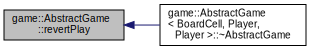
\includegraphics[width=350pt]{classgame_1_1_abstract_game_af6088ae12ed47989dde7f8869e79d934_icgraph}
\end{center}
\end{figure}


\subsection{Member Data Documentation}
\mbox{\Hypertarget{classgame_1_1_abstract_game_a6df5f611daa1731c4c8d3d5e6289e7e5}\label{classgame_1_1_abstract_game_a6df5f611daa1731c4c8d3d5e6289e7e5}} 
\index{game\+::\+Abstract\+Game@{game\+::\+Abstract\+Game}!board@{board}}
\index{board@{board}!game\+::\+Abstract\+Game@{game\+::\+Abstract\+Game}}
\subsubsection{\texorpdfstring{board}{board}}
{\footnotesize\ttfamily template$<$class CellT, class PlayerT, class PawnT$>$ \\
\hyperlink{classgame_1_1_abstract_board}{Abstract\+Board}$<$CellT, PlayerT, PawnT$>$$\ast$ \hyperlink{classgame_1_1_abstract_game}{game\+::\+Abstract\+Game}$<$ CellT, PlayerT, PawnT $>$\+::board}



The documentation for this class was generated from the following files\+:\begin{DoxyCompactItemize}
\item 
/workspace/src/game\+\_\+logic/\hyperlink{_abstract_game_8hpp}{Abstract\+Game.\+hpp}\item 
/workspace/src/game\+\_\+logic/\hyperlink{_abstract_game_8cpp}{Abstract\+Game.\+cpp}\end{DoxyCompactItemize}

\hypertarget{classgame_1_1_abstract_interface}{}\section{game\+:\+:Abstract\+Interface Class Reference}
\label{classgame_1_1_abstract_interface}\index{game\+::\+Abstract\+Interface@{game\+::\+Abstract\+Interface}}


{\ttfamily \#include $<$Abstract\+Interface.\+hpp$>$}



Inheritance diagram for game\+:\+:Abstract\+Interface\+:
\nopagebreak
\begin{figure}[H]
\begin{center}
\leavevmode
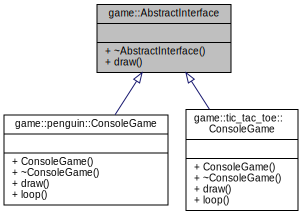
\includegraphics[width=350pt]{classgame_1_1_abstract_interface__inherit__graph}
\end{center}
\end{figure}


Collaboration diagram for game\+:\+:Abstract\+Interface\+:
\nopagebreak
\begin{figure}[H]
\begin{center}
\leavevmode
\includegraphics[width=214pt]{classgame_1_1_abstract_interface__coll__graph}
\end{center}
\end{figure}
\subsection*{Public Member Functions}
\begin{DoxyCompactItemize}
\item 
virtual \hyperlink{classgame_1_1_abstract_interface_a29480586421a44d384932f48aa05f97f}{$\sim$\+Abstract\+Interface} ()
\item 
virtual void \hyperlink{classgame_1_1_abstract_interface_af4330557019768a4be424165e4cf008f}{draw} ()=0
\end{DoxyCompactItemize}


\subsection{Constructor \& Destructor Documentation}
\mbox{\Hypertarget{classgame_1_1_abstract_interface_a29480586421a44d384932f48aa05f97f}\label{classgame_1_1_abstract_interface_a29480586421a44d384932f48aa05f97f}} 
\index{game\+::\+Abstract\+Interface@{game\+::\+Abstract\+Interface}!````~Abstract\+Interface@{$\sim$\+Abstract\+Interface}}
\index{````~Abstract\+Interface@{$\sim$\+Abstract\+Interface}!game\+::\+Abstract\+Interface@{game\+::\+Abstract\+Interface}}
\subsubsection{\texorpdfstring{$\sim$\+Abstract\+Interface()}{~AbstractInterface()}}
{\footnotesize\ttfamily virtual game\+::\+Abstract\+Interface\+::$\sim$\+Abstract\+Interface (\begin{DoxyParamCaption}{ }\end{DoxyParamCaption})\hspace{0.3cm}{\ttfamily [inline]}, {\ttfamily [virtual]}}

Here is the call graph for this function\+:
\nopagebreak
\begin{figure}[H]
\begin{center}
\leavevmode
\includegraphics[width=350pt]{classgame_1_1_abstract_interface_a29480586421a44d384932f48aa05f97f_cgraph}
\end{center}
\end{figure}


\subsection{Member Function Documentation}
\mbox{\Hypertarget{classgame_1_1_abstract_interface_af4330557019768a4be424165e4cf008f}\label{classgame_1_1_abstract_interface_af4330557019768a4be424165e4cf008f}} 
\index{game\+::\+Abstract\+Interface@{game\+::\+Abstract\+Interface}!draw@{draw}}
\index{draw@{draw}!game\+::\+Abstract\+Interface@{game\+::\+Abstract\+Interface}}
\subsubsection{\texorpdfstring{draw()}{draw()}}
{\footnotesize\ttfamily virtual void game\+::\+Abstract\+Interface\+::draw (\begin{DoxyParamCaption}{ }\end{DoxyParamCaption})\hspace{0.3cm}{\ttfamily [pure virtual]}}



Implemented in \hyperlink{classgame_1_1penguin_1_1_console_game_a71c697742201f71b29327bf8554c2ef0}{game\+::penguin\+::\+Console\+Game}, and \hyperlink{classgame_1_1tic__tac__toe_1_1_console_game_a209ec289b23e0325417d50a31a323b37}{game\+::tic\+\_\+tac\+\_\+toe\+::\+Console\+Game}.

Here is the caller graph for this function\+:
\nopagebreak
\begin{figure}[H]
\begin{center}
\leavevmode
\includegraphics[width=350pt]{classgame_1_1_abstract_interface_af4330557019768a4be424165e4cf008f_icgraph}
\end{center}
\end{figure}


The documentation for this class was generated from the following file\+:\begin{DoxyCompactItemize}
\item 
/workspace/src/game\+\_\+logic/\hyperlink{_abstract_interface_8hpp}{Abstract\+Interface.\+hpp}\end{DoxyCompactItemize}

\hypertarget{classgame_1_1_abstract_pawn}{}\section{game\+:\+:Abstract\+Pawn$<$ PlayerT, CellT $>$ Class Template Reference}
\label{classgame_1_1_abstract_pawn}\index{game\+::\+Abstract\+Pawn$<$ Player\+T, Cell\+T $>$@{game\+::\+Abstract\+Pawn$<$ Player\+T, Cell\+T $>$}}


{\ttfamily \#include $<$Abstract\+Pawn.\+hpp$>$}



Inheritance diagram for game\+:\+:Abstract\+Pawn$<$ PlayerT, CellT $>$\+:
\nopagebreak
\begin{figure}[H]
\begin{center}
\leavevmode
\includegraphics[width=350pt]{classgame_1_1_abstract_pawn__inherit__graph}
\end{center}
\end{figure}


Collaboration diagram for game\+:\+:Abstract\+Pawn$<$ PlayerT, CellT $>$\+:
\nopagebreak
\begin{figure}[H]
\begin{center}
\leavevmode
\includegraphics[width=196pt]{classgame_1_1_abstract_pawn__coll__graph}
\end{center}
\end{figure}
\subsection*{Public Member Functions}
\begin{DoxyCompactItemize}
\item 
\hyperlink{classgame_1_1_abstract_pawn_af1bc0b6647a170f6d4be38a6475757e3}{Abstract\+Pawn} (unsigned int id, PlayerT \&owner)
\item 
\hyperlink{classgame_1_1_abstract_pawn_af83fab32ac2e13daf3c693d465a061ed}{Abstract\+Pawn} (const \hyperlink{classgame_1_1_abstract_pawn}{Abstract\+Pawn}$<$ PlayerT, CellT $>$ \&)=delete
\item 
virtual \hyperlink{classgame_1_1_abstract_pawn_a3fa5336d077fb00b3b3df2bc662e62eb}{$\sim$\+Abstract\+Pawn} ()
\item 
PlayerT $\ast$ \hyperlink{classgame_1_1_abstract_pawn_aac49fdd8bd4aa4386fd47d3f6993b8df}{get\+Owner} () const
\item 
unsigned int \hyperlink{classgame_1_1_abstract_pawn_a49354506912d0e1bf5272627aa2bc86e}{get\+Id} () const
\begin{DoxyCompactList}\small\item\em Get pawn\textquotesingle{}s id. \end{DoxyCompactList}\item 
void \hyperlink{classgame_1_1_abstract_pawn_a678ab4c2f0191bafa3e1e16cf04fa9d0}{set\+Current\+Cell} (CellT $\ast$cell)
\begin{DoxyCompactList}\small\item\em Queue the move done at the top of the stack. \end{DoxyCompactList}\item 
CellT $\ast$ \hyperlink{classgame_1_1_abstract_pawn_ae9ad3bf0ee738571d0dd5992feae6bb7}{get\+Current\+Cell} () const
\item 
bool \hyperlink{classgame_1_1_abstract_pawn_a65dada55fadc0df1169d8a6b0661c05a}{operator==} (const \hyperlink{classgame_1_1_abstract_pawn}{Abstract\+Pawn}$<$ PlayerT, CellT $>$ \&pawn) const
\item 
bool \hyperlink{classgame_1_1_abstract_pawn_a8c5ef6187be3592d15ba9cf6a433c91c}{operator!=} (const \hyperlink{classgame_1_1_abstract_pawn}{Abstract\+Pawn}$<$ PlayerT, CellT $>$ \&pawn) const
\end{DoxyCompactItemize}
\subsection*{Protected Member Functions}
\begin{DoxyCompactItemize}
\item 
virtual bool \hyperlink{classgame_1_1_abstract_pawn_aa1911c1f88d6b345a4a004cded7e6904}{equals\+\_\+to} (const \hyperlink{classgame_1_1_abstract_pawn}{Abstract\+Pawn}$<$ PlayerT, CellT $>$ \&pawn) const
\end{DoxyCompactItemize}


\subsection{Constructor \& Destructor Documentation}
\mbox{\Hypertarget{classgame_1_1_abstract_pawn_af1bc0b6647a170f6d4be38a6475757e3}\label{classgame_1_1_abstract_pawn_af1bc0b6647a170f6d4be38a6475757e3}} 
\index{game\+::\+Abstract\+Pawn@{game\+::\+Abstract\+Pawn}!Abstract\+Pawn@{Abstract\+Pawn}}
\index{Abstract\+Pawn@{Abstract\+Pawn}!game\+::\+Abstract\+Pawn@{game\+::\+Abstract\+Pawn}}
\subsubsection{\texorpdfstring{Abstract\+Pawn()}{AbstractPawn()}\hspace{0.1cm}{\footnotesize\ttfamily [1/2]}}
{\footnotesize\ttfamily template$<$class PlayerT, class CellT $>$ \\
\hyperlink{classgame_1_1_abstract_pawn}{game\+::\+Abstract\+Pawn}$<$ PlayerT, CellT $>$\+::\hyperlink{classgame_1_1_abstract_pawn}{Abstract\+Pawn} (\begin{DoxyParamCaption}\item[{unsigned int}]{id,  }\item[{PlayerT \&}]{owner }\end{DoxyParamCaption})\hspace{0.3cm}{\ttfamily [explicit]}}

\mbox{\Hypertarget{classgame_1_1_abstract_pawn_af83fab32ac2e13daf3c693d465a061ed}\label{classgame_1_1_abstract_pawn_af83fab32ac2e13daf3c693d465a061ed}} 
\index{game\+::\+Abstract\+Pawn@{game\+::\+Abstract\+Pawn}!Abstract\+Pawn@{Abstract\+Pawn}}
\index{Abstract\+Pawn@{Abstract\+Pawn}!game\+::\+Abstract\+Pawn@{game\+::\+Abstract\+Pawn}}
\subsubsection{\texorpdfstring{Abstract\+Pawn()}{AbstractPawn()}\hspace{0.1cm}{\footnotesize\ttfamily [2/2]}}
{\footnotesize\ttfamily template$<$class PlayerT, class CellT$>$ \\
\hyperlink{classgame_1_1_abstract_pawn}{game\+::\+Abstract\+Pawn}$<$ PlayerT, CellT $>$\+::\hyperlink{classgame_1_1_abstract_pawn}{Abstract\+Pawn} (\begin{DoxyParamCaption}\item[{const \hyperlink{classgame_1_1_abstract_pawn}{Abstract\+Pawn}$<$ PlayerT, CellT $>$ \&}]{ }\end{DoxyParamCaption})\hspace{0.3cm}{\ttfamily [explicit]}, {\ttfamily [delete]}}

\mbox{\Hypertarget{classgame_1_1_abstract_pawn_a3fa5336d077fb00b3b3df2bc662e62eb}\label{classgame_1_1_abstract_pawn_a3fa5336d077fb00b3b3df2bc662e62eb}} 
\index{game\+::\+Abstract\+Pawn@{game\+::\+Abstract\+Pawn}!````~Abstract\+Pawn@{$\sim$\+Abstract\+Pawn}}
\index{````~Abstract\+Pawn@{$\sim$\+Abstract\+Pawn}!game\+::\+Abstract\+Pawn@{game\+::\+Abstract\+Pawn}}
\subsubsection{\texorpdfstring{$\sim$\+Abstract\+Pawn()}{~AbstractPawn()}}
{\footnotesize\ttfamily template$<$class PlayerT, class CellT$>$ \\
virtual \hyperlink{classgame_1_1_abstract_pawn}{game\+::\+Abstract\+Pawn}$<$ PlayerT, CellT $>$\+::$\sim$\hyperlink{classgame_1_1_abstract_pawn}{Abstract\+Pawn} (\begin{DoxyParamCaption}{ }\end{DoxyParamCaption})\hspace{0.3cm}{\ttfamily [inline]}, {\ttfamily [virtual]}}



\subsection{Member Function Documentation}
\mbox{\Hypertarget{classgame_1_1_abstract_pawn_aa1911c1f88d6b345a4a004cded7e6904}\label{classgame_1_1_abstract_pawn_aa1911c1f88d6b345a4a004cded7e6904}} 
\index{game\+::\+Abstract\+Pawn@{game\+::\+Abstract\+Pawn}!equals\+\_\+to@{equals\+\_\+to}}
\index{equals\+\_\+to@{equals\+\_\+to}!game\+::\+Abstract\+Pawn@{game\+::\+Abstract\+Pawn}}
\subsubsection{\texorpdfstring{equals\+\_\+to()}{equals\_to()}}
{\footnotesize\ttfamily template$<$class PlayerT, class CellT$>$ \\
bool \hyperlink{classgame_1_1_abstract_pawn}{game\+::\+Abstract\+Pawn}$<$ PlayerT, CellT $>$\+::equals\+\_\+to (\begin{DoxyParamCaption}\item[{const \hyperlink{classgame_1_1_abstract_pawn}{Abstract\+Pawn}$<$ PlayerT, CellT $>$ \&}]{pawn }\end{DoxyParamCaption}) const\hspace{0.3cm}{\ttfamily [protected]}, {\ttfamily [virtual]}}

Here is the caller graph for this function\+:
\nopagebreak
\begin{figure}[H]
\begin{center}
\leavevmode
\includegraphics[width=348pt]{classgame_1_1_abstract_pawn_aa1911c1f88d6b345a4a004cded7e6904_icgraph}
\end{center}
\end{figure}
\mbox{\Hypertarget{classgame_1_1_abstract_pawn_ae9ad3bf0ee738571d0dd5992feae6bb7}\label{classgame_1_1_abstract_pawn_ae9ad3bf0ee738571d0dd5992feae6bb7}} 
\index{game\+::\+Abstract\+Pawn@{game\+::\+Abstract\+Pawn}!get\+Current\+Cell@{get\+Current\+Cell}}
\index{get\+Current\+Cell@{get\+Current\+Cell}!game\+::\+Abstract\+Pawn@{game\+::\+Abstract\+Pawn}}
\subsubsection{\texorpdfstring{get\+Current\+Cell()}{getCurrentCell()}}
{\footnotesize\ttfamily template$<$class PlayerT , class CellT $>$ \\
CellT $\ast$ \hyperlink{classgame_1_1_abstract_pawn}{game\+::\+Abstract\+Pawn}$<$ PlayerT, CellT $>$\+::get\+Current\+Cell (\begin{DoxyParamCaption}{ }\end{DoxyParamCaption}) const}

Here is the caller graph for this function\+:
\nopagebreak
\begin{figure}[H]
\begin{center}
\leavevmode
\includegraphics[width=350pt]{classgame_1_1_abstract_pawn_ae9ad3bf0ee738571d0dd5992feae6bb7_icgraph}
\end{center}
\end{figure}
\mbox{\Hypertarget{classgame_1_1_abstract_pawn_a49354506912d0e1bf5272627aa2bc86e}\label{classgame_1_1_abstract_pawn_a49354506912d0e1bf5272627aa2bc86e}} 
\index{game\+::\+Abstract\+Pawn@{game\+::\+Abstract\+Pawn}!get\+Id@{get\+Id}}
\index{get\+Id@{get\+Id}!game\+::\+Abstract\+Pawn@{game\+::\+Abstract\+Pawn}}
\subsubsection{\texorpdfstring{get\+Id()}{getId()}}
{\footnotesize\ttfamily template$<$class PlayerT, class CellT$>$ \\
unsigned int \hyperlink{classgame_1_1_abstract_pawn}{game\+::\+Abstract\+Pawn}$<$ PlayerT, CellT $>$\+::get\+Id (\begin{DoxyParamCaption}{ }\end{DoxyParamCaption}) const\hspace{0.3cm}{\ttfamily [inline]}}



Get pawn\textquotesingle{}s id. 

\begin{DoxyReturn}{Returns}
constexpr unsigned int the id 
\end{DoxyReturn}
Here is the caller graph for this function\+:
\nopagebreak
\begin{figure}[H]
\begin{center}
\leavevmode
\includegraphics[width=350pt]{classgame_1_1_abstract_pawn_a49354506912d0e1bf5272627aa2bc86e_icgraph}
\end{center}
\end{figure}
\mbox{\Hypertarget{classgame_1_1_abstract_pawn_aac49fdd8bd4aa4386fd47d3f6993b8df}\label{classgame_1_1_abstract_pawn_aac49fdd8bd4aa4386fd47d3f6993b8df}} 
\index{game\+::\+Abstract\+Pawn@{game\+::\+Abstract\+Pawn}!get\+Owner@{get\+Owner}}
\index{get\+Owner@{get\+Owner}!game\+::\+Abstract\+Pawn@{game\+::\+Abstract\+Pawn}}
\subsubsection{\texorpdfstring{get\+Owner()}{getOwner()}}
{\footnotesize\ttfamily template$<$class PlayerT, class CellT$>$ \\
PlayerT$\ast$ \hyperlink{classgame_1_1_abstract_pawn}{game\+::\+Abstract\+Pawn}$<$ PlayerT, CellT $>$\+::get\+Owner (\begin{DoxyParamCaption}{ }\end{DoxyParamCaption}) const\hspace{0.3cm}{\ttfamily [inline]}}

Here is the caller graph for this function\+:
\nopagebreak
\begin{figure}[H]
\begin{center}
\leavevmode
\includegraphics[width=350pt]{classgame_1_1_abstract_pawn_aac49fdd8bd4aa4386fd47d3f6993b8df_icgraph}
\end{center}
\end{figure}
\mbox{\Hypertarget{classgame_1_1_abstract_pawn_a8c5ef6187be3592d15ba9cf6a433c91c}\label{classgame_1_1_abstract_pawn_a8c5ef6187be3592d15ba9cf6a433c91c}} 
\index{game\+::\+Abstract\+Pawn@{game\+::\+Abstract\+Pawn}!operator"!=@{operator"!=}}
\index{operator"!=@{operator"!=}!game\+::\+Abstract\+Pawn@{game\+::\+Abstract\+Pawn}}
\subsubsection{\texorpdfstring{operator"!=()}{operator!=()}}
{\footnotesize\ttfamily template$<$class PlayerT, class CellT$>$ \\
bool \hyperlink{classgame_1_1_abstract_pawn}{game\+::\+Abstract\+Pawn}$<$ PlayerT, CellT $>$\+::operator!= (\begin{DoxyParamCaption}\item[{const \hyperlink{classgame_1_1_abstract_pawn}{Abstract\+Pawn}$<$ PlayerT, CellT $>$ \&}]{pawn }\end{DoxyParamCaption}) const\hspace{0.3cm}{\ttfamily [inline]}}

\mbox{\Hypertarget{classgame_1_1_abstract_pawn_a65dada55fadc0df1169d8a6b0661c05a}\label{classgame_1_1_abstract_pawn_a65dada55fadc0df1169d8a6b0661c05a}} 
\index{game\+::\+Abstract\+Pawn@{game\+::\+Abstract\+Pawn}!operator==@{operator==}}
\index{operator==@{operator==}!game\+::\+Abstract\+Pawn@{game\+::\+Abstract\+Pawn}}
\subsubsection{\texorpdfstring{operator==()}{operator==()}}
{\footnotesize\ttfamily template$<$class PlayerT, class CellT$>$ \\
bool \hyperlink{classgame_1_1_abstract_pawn}{game\+::\+Abstract\+Pawn}$<$ PlayerT, CellT $>$\+::operator== (\begin{DoxyParamCaption}\item[{const \hyperlink{classgame_1_1_abstract_pawn}{Abstract\+Pawn}$<$ PlayerT, CellT $>$ \&}]{pawn }\end{DoxyParamCaption}) const\hspace{0.3cm}{\ttfamily [inline]}}

\mbox{\Hypertarget{classgame_1_1_abstract_pawn_a678ab4c2f0191bafa3e1e16cf04fa9d0}\label{classgame_1_1_abstract_pawn_a678ab4c2f0191bafa3e1e16cf04fa9d0}} 
\index{game\+::\+Abstract\+Pawn@{game\+::\+Abstract\+Pawn}!set\+Current\+Cell@{set\+Current\+Cell}}
\index{set\+Current\+Cell@{set\+Current\+Cell}!game\+::\+Abstract\+Pawn@{game\+::\+Abstract\+Pawn}}
\subsubsection{\texorpdfstring{set\+Current\+Cell()}{setCurrentCell()}}
{\footnotesize\ttfamily template$<$class PlayerT , class CellT$>$ \\
void \hyperlink{classgame_1_1_abstract_pawn}{game\+::\+Abstract\+Pawn}$<$ PlayerT, CellT $>$\+::set\+Current\+Cell (\begin{DoxyParamCaption}\item[{CellT $\ast$}]{cell }\end{DoxyParamCaption})}



Queue the move done at the top of the stack. 


\begin{DoxyParams}{Parameters}
{\em move} & the move to stack \\
\hline
\end{DoxyParams}
Here is the caller graph for this function\+:
\nopagebreak
\begin{figure}[H]
\begin{center}
\leavevmode
\includegraphics[width=350pt]{classgame_1_1_abstract_pawn_a678ab4c2f0191bafa3e1e16cf04fa9d0_icgraph}
\end{center}
\end{figure}


The documentation for this class was generated from the following files\+:\begin{DoxyCompactItemize}
\item 
/workspace/src/game\+\_\+logic/\hyperlink{_abstract_pawn_8hpp}{Abstract\+Pawn.\+hpp}\item 
/workspace/src/game\+\_\+logic/\hyperlink{_abstract_pawn_8cpp}{Abstract\+Pawn.\+cpp}\end{DoxyCompactItemize}

\hypertarget{classgame_1_1_abstract_player}{}\section{game\+:\+:Abstract\+Player Class Reference}
\label{classgame_1_1_abstract_player}\index{game\+::\+Abstract\+Player@{game\+::\+Abstract\+Player}}


{\ttfamily \#include $<$Abstract\+Player.\+hpp$>$}



Inheritance diagram for game\+:\+:Abstract\+Player\+:
\nopagebreak
\begin{figure}[H]
\begin{center}
\leavevmode
\includegraphics[width=350pt]{classgame_1_1_abstract_player__inherit__graph}
\end{center}
\end{figure}


Collaboration diagram for game\+:\+:Abstract\+Player\+:
\nopagebreak
\begin{figure}[H]
\begin{center}
\leavevmode
\includegraphics[width=202pt]{classgame_1_1_abstract_player__coll__graph}
\end{center}
\end{figure}
\subsection*{Public Member Functions}
\begin{DoxyCompactItemize}
\item 
\hyperlink{classgame_1_1_abstract_player_a7164932ca617a90d1b67a58b6d32e095}{Abstract\+Player} (unsigned int id)
\begin{DoxyCompactList}\small\item\em Construct a new Abstract Player object. \end{DoxyCompactList}\item 
\hyperlink{classgame_1_1_abstract_player_aa2ee6723a58b2432368d845c16ca978f}{Abstract\+Player} (const \hyperlink{classgame_1_1_abstract_player}{Abstract\+Player} \&)=default
\item 
virtual \hyperlink{classgame_1_1_abstract_player_a0943c270c648d668b696757004955d72}{$\sim$\+Abstract\+Player} ()
\item 
unsigned int \hyperlink{classgame_1_1_abstract_player_a88e33e40f98283588a535f66bf1b6640}{get\+Id} () const
\begin{DoxyCompactList}\small\item\em Get player\textquotesingle{}s id. \end{DoxyCompactList}\item 
bool \hyperlink{classgame_1_1_abstract_player_aaffd1859f7b8b2cd3a00fc47432800e4}{operator==} (const \hyperlink{classgame_1_1_abstract_player}{Abstract\+Player} \&player) const
\item 
bool \hyperlink{classgame_1_1_abstract_player_a3c88c5ef8f89fd74b3e48ff636049c94}{operator!=} (const \hyperlink{classgame_1_1_abstract_player}{Abstract\+Player} \&player) const
\end{DoxyCompactItemize}
\subsection*{Protected Member Functions}
\begin{DoxyCompactItemize}
\item 
virtual bool \hyperlink{classgame_1_1_abstract_player_adacb7220ee80c15058b9e2619bd9c72b}{equals\+\_\+to} (const \hyperlink{classgame_1_1_abstract_player}{Abstract\+Player} \&player) const
\end{DoxyCompactItemize}


\subsection{Constructor \& Destructor Documentation}
\mbox{\Hypertarget{classgame_1_1_abstract_player_a7164932ca617a90d1b67a58b6d32e095}\label{classgame_1_1_abstract_player_a7164932ca617a90d1b67a58b6d32e095}} 
\index{game\+::\+Abstract\+Player@{game\+::\+Abstract\+Player}!Abstract\+Player@{Abstract\+Player}}
\index{Abstract\+Player@{Abstract\+Player}!game\+::\+Abstract\+Player@{game\+::\+Abstract\+Player}}
\subsubsection{\texorpdfstring{Abstract\+Player()}{AbstractPlayer()}\hspace{0.1cm}{\footnotesize\ttfamily [1/2]}}
{\footnotesize\ttfamily game\+::\+Abstract\+Player\+::\+Abstract\+Player (\begin{DoxyParamCaption}\item[{unsigned int}]{id }\end{DoxyParamCaption})\hspace{0.3cm}{\ttfamily [explicit]}}



Construct a new Abstract Player object. 


\begin{DoxyParams}{Parameters}
{\em id} & the id of the player \\
\hline
\end{DoxyParams}
\mbox{\Hypertarget{classgame_1_1_abstract_player_aa2ee6723a58b2432368d845c16ca978f}\label{classgame_1_1_abstract_player_aa2ee6723a58b2432368d845c16ca978f}} 
\index{game\+::\+Abstract\+Player@{game\+::\+Abstract\+Player}!Abstract\+Player@{Abstract\+Player}}
\index{Abstract\+Player@{Abstract\+Player}!game\+::\+Abstract\+Player@{game\+::\+Abstract\+Player}}
\subsubsection{\texorpdfstring{Abstract\+Player()}{AbstractPlayer()}\hspace{0.1cm}{\footnotesize\ttfamily [2/2]}}
{\footnotesize\ttfamily game\+::\+Abstract\+Player\+::\+Abstract\+Player (\begin{DoxyParamCaption}\item[{const \hyperlink{classgame_1_1_abstract_player}{Abstract\+Player} \&}]{ }\end{DoxyParamCaption})\hspace{0.3cm}{\ttfamily [explicit]}, {\ttfamily [default]}}

\mbox{\Hypertarget{classgame_1_1_abstract_player_a0943c270c648d668b696757004955d72}\label{classgame_1_1_abstract_player_a0943c270c648d668b696757004955d72}} 
\index{game\+::\+Abstract\+Player@{game\+::\+Abstract\+Player}!````~Abstract\+Player@{$\sim$\+Abstract\+Player}}
\index{````~Abstract\+Player@{$\sim$\+Abstract\+Player}!game\+::\+Abstract\+Player@{game\+::\+Abstract\+Player}}
\subsubsection{\texorpdfstring{$\sim$\+Abstract\+Player()}{~AbstractPlayer()}}
{\footnotesize\ttfamily virtual game\+::\+Abstract\+Player\+::$\sim$\+Abstract\+Player (\begin{DoxyParamCaption}{ }\end{DoxyParamCaption})\hspace{0.3cm}{\ttfamily [inline]}, {\ttfamily [virtual]}}



\subsection{Member Function Documentation}
\mbox{\Hypertarget{classgame_1_1_abstract_player_adacb7220ee80c15058b9e2619bd9c72b}\label{classgame_1_1_abstract_player_adacb7220ee80c15058b9e2619bd9c72b}} 
\index{game\+::\+Abstract\+Player@{game\+::\+Abstract\+Player}!equals\+\_\+to@{equals\+\_\+to}}
\index{equals\+\_\+to@{equals\+\_\+to}!game\+::\+Abstract\+Player@{game\+::\+Abstract\+Player}}
\subsubsection{\texorpdfstring{equals\+\_\+to()}{equals\_to()}}
{\footnotesize\ttfamily bool game\+::\+Abstract\+Player\+::equals\+\_\+to (\begin{DoxyParamCaption}\item[{const \hyperlink{classgame_1_1_abstract_player}{Abstract\+Player} \&}]{player }\end{DoxyParamCaption}) const\hspace{0.3cm}{\ttfamily [protected]}, {\ttfamily [virtual]}}



Reimplemented in \hyperlink{classgame_1_1penguin_1_1_human_player_ad0f5548eee1fb7b866c592da4b529b69}{game\+::penguin\+::\+Human\+Player}.

Here is the caller graph for this function\+:
\nopagebreak
\begin{figure}[H]
\begin{center}
\leavevmode
\includegraphics[width=350pt]{classgame_1_1_abstract_player_adacb7220ee80c15058b9e2619bd9c72b_icgraph}
\end{center}
\end{figure}
\mbox{\Hypertarget{classgame_1_1_abstract_player_a88e33e40f98283588a535f66bf1b6640}\label{classgame_1_1_abstract_player_a88e33e40f98283588a535f66bf1b6640}} 
\index{game\+::\+Abstract\+Player@{game\+::\+Abstract\+Player}!get\+Id@{get\+Id}}
\index{get\+Id@{get\+Id}!game\+::\+Abstract\+Player@{game\+::\+Abstract\+Player}}
\subsubsection{\texorpdfstring{get\+Id()}{getId()}}
{\footnotesize\ttfamily unsigned int game\+::\+Abstract\+Player\+::get\+Id (\begin{DoxyParamCaption}{ }\end{DoxyParamCaption}) const\hspace{0.3cm}{\ttfamily [inline]}}



Get player\textquotesingle{}s id. 

\begin{DoxyReturn}{Returns}
constexpr unsigned int the id 
\end{DoxyReturn}
Here is the caller graph for this function\+:
\nopagebreak
\begin{figure}[H]
\begin{center}
\leavevmode
\includegraphics[width=350pt]{classgame_1_1_abstract_player_a88e33e40f98283588a535f66bf1b6640_icgraph}
\end{center}
\end{figure}
\mbox{\Hypertarget{classgame_1_1_abstract_player_a3c88c5ef8f89fd74b3e48ff636049c94}\label{classgame_1_1_abstract_player_a3c88c5ef8f89fd74b3e48ff636049c94}} 
\index{game\+::\+Abstract\+Player@{game\+::\+Abstract\+Player}!operator"!=@{operator"!=}}
\index{operator"!=@{operator"!=}!game\+::\+Abstract\+Player@{game\+::\+Abstract\+Player}}
\subsubsection{\texorpdfstring{operator"!=()}{operator!=()}}
{\footnotesize\ttfamily bool game\+::\+Abstract\+Player\+::operator!= (\begin{DoxyParamCaption}\item[{const \hyperlink{classgame_1_1_abstract_player}{Abstract\+Player} \&}]{player }\end{DoxyParamCaption}) const\hspace{0.3cm}{\ttfamily [inline]}}

Here is the call graph for this function\+:
\nopagebreak
\begin{figure}[H]
\begin{center}
\leavevmode
\includegraphics[width=350pt]{classgame_1_1_abstract_player_a3c88c5ef8f89fd74b3e48ff636049c94_cgraph}
\end{center}
\end{figure}
\mbox{\Hypertarget{classgame_1_1_abstract_player_aaffd1859f7b8b2cd3a00fc47432800e4}\label{classgame_1_1_abstract_player_aaffd1859f7b8b2cd3a00fc47432800e4}} 
\index{game\+::\+Abstract\+Player@{game\+::\+Abstract\+Player}!operator==@{operator==}}
\index{operator==@{operator==}!game\+::\+Abstract\+Player@{game\+::\+Abstract\+Player}}
\subsubsection{\texorpdfstring{operator==()}{operator==()}}
{\footnotesize\ttfamily bool game\+::\+Abstract\+Player\+::operator== (\begin{DoxyParamCaption}\item[{const \hyperlink{classgame_1_1_abstract_player}{Abstract\+Player} \&}]{player }\end{DoxyParamCaption}) const\hspace{0.3cm}{\ttfamily [inline]}}

Here is the call graph for this function\+:
\nopagebreak
\begin{figure}[H]
\begin{center}
\leavevmode
\includegraphics[width=350pt]{classgame_1_1_abstract_player_aaffd1859f7b8b2cd3a00fc47432800e4_cgraph}
\end{center}
\end{figure}


The documentation for this class was generated from the following files\+:\begin{DoxyCompactItemize}
\item 
/workspace/src/game\+\_\+logic/\hyperlink{_abstract_player_8hpp}{Abstract\+Player.\+hpp}\item 
/workspace/src/game\+\_\+logic/\hyperlink{_abstract_player_8cpp}{Abstract\+Player.\+cpp}\end{DoxyCompactItemize}

\hypertarget{classgame_1_1penguin_1_1_board}{}\section{game\+:\+:penguin\+:\+:Board Class Reference}
\label{classgame_1_1penguin_1_1_board}\index{game\+::penguin\+::\+Board@{game\+::penguin\+::\+Board}}


Describes the hexagonal board of the game, based on an axial coordinate system.  




{\ttfamily \#include $<$Board.\+hpp$>$}



Inheritance diagram for game\+:\+:penguin\+:\+:Board\+:
\nopagebreak
\begin{figure}[H]
\begin{center}
\leavevmode
\includegraphics[height=550pt]{classgame_1_1penguin_1_1_board__inherit__graph}
\end{center}
\end{figure}


Collaboration diagram for game\+:\+:penguin\+:\+:Board\+:
\nopagebreak
\begin{figure}[H]
\begin{center}
\leavevmode
\includegraphics[height=550pt]{classgame_1_1penguin_1_1_board__coll__graph}
\end{center}
\end{figure}
\subsection*{Public Member Functions}
\begin{DoxyCompactItemize}
\item 
\hyperlink{classgame_1_1penguin_1_1_board_aea5bd314dbc295e71759baf2051409c5}{Board} (const size\+\_\+t dimension, const size\+\_\+t number\+\_\+of\+\_\+penguins\+\_\+per\+\_\+team)
\begin{DoxyCompactList}\small\item\em Construct a new \hyperlink{classgame_1_1penguin_1_1_board}{Board} object. \end{DoxyCompactList}\item 
\hyperlink{classgame_1_1penguin_1_1_board_a7768c6b6dab42e72a3f3853af2ad1f5a}{$\sim$\+Board} ()
\begin{DoxyCompactList}\small\item\em Destroy the \hyperlink{classgame_1_1penguin_1_1_board}{Board} object. \end{DoxyCompactList}\item 
bool \hyperlink{classgame_1_1penguin_1_1_board_af297dc572afb02dafc61e3b8e849338f}{perform\+Move} (\hyperlink{classgame_1_1penguin_1_1_penguin_pawn}{Penguin\+Pawn} $\ast$pawn, \hyperlink{classgame_1_1penguin_1_1_board_cell}{Board\+Cell} $\ast$cell) override
\begin{DoxyCompactList}\small\item\em Performs a particular move. \end{DoxyCompactList}\item 
const \hyperlink{structgame_1_1_move}{Move}$<$ \hyperlink{classgame_1_1penguin_1_1_board_cell}{Board\+Cell}, \hyperlink{classgame_1_1penguin_1_1_penguin_pawn}{Penguin\+Pawn} $>$ \hyperlink{classgame_1_1penguin_1_1_board_a45ecb5bba50b4d03592ac4ddf9255b49}{revert\+Move} () override
\begin{DoxyCompactList}\small\item\em Revert the last move made on the behalf of the human player. \end{DoxyCompactList}\item 
int \hyperlink{classgame_1_1penguin_1_1_board_a3d659743bc33b43168c82dc4e2d3b00e}{check\+Status} () override
\begin{DoxyCompactList}\small\item\em Chek wether or not the game is finished. \end{DoxyCompactList}\item 
bool \hyperlink{classgame_1_1penguin_1_1_board_ae85ef3019829098c5ad5afb1c3ebceb5}{is\+Able\+To\+Move} (const \hyperlink{classgame_1_1penguin_1_1_human_player}{Human\+Player} $\ast$const \&player)
\begin{DoxyCompactList}\small\item\em Is the player able to move. \end{DoxyCompactList}\item 
std\+::vector$<$ \hyperlink{classgame_1_1penguin_1_1_board_cell}{Board\+Cell} $\ast$ $>$ \hyperlink{classgame_1_1penguin_1_1_board_a26bc6f1c2da1197d9b68f9b4c4e3126b}{get\+Available\+Cells} (\hyperlink{classgame_1_1penguin_1_1_penguin_pawn}{Penguin\+Pawn} $\ast$penguin) override
\begin{DoxyCompactList}\small\item\em Get a list of available cells, ie player can move onto. \end{DoxyCompactList}\item 
std\+::vector$<$ \hyperlink{classgame_1_1penguin_1_1_board_cell}{Board\+Cell} $\ast$ $>$ \hyperlink{classgame_1_1penguin_1_1_board_afae3ac9e82200303d28dd4cf7bfa12ec}{get\+Board\+Cells} () override
\begin{DoxyCompactList}\small\item\em Get a list of all cells. \end{DoxyCompactList}\item 
size\+\_\+t \hyperlink{classgame_1_1penguin_1_1_board_a7636e3bdb2da72d2a6395b1a2d846394}{size} () const override
\item 
\hyperlink{classgame_1_1penguin_1_1_board_cell}{Board\+Cell} $\ast$ \hyperlink{classgame_1_1penguin_1_1_board_ac9fbe04a302208fcb5f66e717182b6d4}{get\+Cell} (int xx, int yy) override
\begin{DoxyCompactList}\small\item\em Get the Cell. \end{DoxyCompactList}\item 
std\+::vector$<$ \hyperlink{classgame_1_1penguin_1_1_penguin_pawn}{Penguin\+Pawn} $\ast$ $>$ \hyperlink{classgame_1_1penguin_1_1_board_a13a38d7c935dd363d7ec9394488539ee}{get\+Pawns\+On\+Board} () override
\begin{DoxyCompactList}\small\item\em Get the Players that are presently palying on the board. \end{DoxyCompactList}\item 
\hyperlink{classgame_1_1penguin_1_1_penguin_pawn}{Penguin\+Pawn} $\ast$ \hyperlink{classgame_1_1penguin_1_1_board_acae84c13dacef3bd988d1ea9a41d055f}{get\+Pawn\+By\+Id} (const unsigned int penguin\+\_\+id) override
\begin{DoxyCompactList}\small\item\em Get a player by it\textquotesingle{}s id. \end{DoxyCompactList}\item 
\hyperlink{classgame_1_1penguin_1_1_penguin_pawn}{Penguin\+Pawn} $\ast$ \hyperlink{classgame_1_1penguin_1_1_board_a169a4af29387bc09929e12af674adc62}{get\+Pawn\+By\+Id} (const unsigned int \&penguin\+\_\+id) const
\item 
\hyperlink{classgame_1_1penguin_1_1_human_player}{Human\+Player} $\ast$ \hyperlink{classgame_1_1penguin_1_1_board_a8728b4381bc2e007710d275bb226cf95}{get\+Player\+By\+Id} (const unsigned int human\+\_\+player\+\_\+id) override
\begin{DoxyCompactList}\small\item\em Gets the player corresponding to a certain id. \end{DoxyCompactList}\item 
\hyperlink{classgame_1_1_abstract_board}{Abstract\+Board}$<$ \hyperlink{classgame_1_1penguin_1_1_board_cell}{Board\+Cell}, \hyperlink{classgame_1_1penguin_1_1_human_player}{Human\+Player}, \hyperlink{classgame_1_1penguin_1_1_penguin_pawn}{Penguin\+Pawn} $>$ $\ast$ \hyperlink{classgame_1_1penguin_1_1_board_acad4a3c7bee2103aea4586356ceabb8e}{clone} () const override
\end{DoxyCompactItemize}
\subsection*{Protected Member Functions}
\begin{DoxyCompactItemize}
\item 
bool \hyperlink{classgame_1_1penguin_1_1_board_a2864b1af9dbdf19273185c504257435c}{check\+For\+Correctness} (const \hyperlink{structgame_1_1_position}{Position} \&start, const \hyperlink{structgame_1_1_position}{Position} \&destination)
\begin{DoxyCompactList}\small\item\em Checks wether or not the move is allowed to be performed. \end{DoxyCompactList}\end{DoxyCompactItemize}
\subsection*{Protected Attributes}
\begin{DoxyCompactItemize}
\item 
\hyperlink{namespacegame_1_1penguin_a6ea7c0fc4c04931bf39fcac439c92735}{penguin\+\_\+board\+\_\+map\+\_\+t} \hyperlink{classgame_1_1penguin_1_1_board_ab89d4ad0fcac9a4cb2ebebb3d0aa3eed}{board\+Values}
\begin{DoxyCompactList}\small\item\em Array of the cell const pointers to variable element indexed in board\+Values. \end{DoxyCompactList}\end{DoxyCompactItemize}


\subsection{Detailed Description}
Describes the hexagonal board of the game, based on an axial coordinate system. 

\subsection{Constructor \& Destructor Documentation}
\mbox{\Hypertarget{classgame_1_1penguin_1_1_board_aea5bd314dbc295e71759baf2051409c5}\label{classgame_1_1penguin_1_1_board_aea5bd314dbc295e71759baf2051409c5}} 
\index{game\+::penguin\+::\+Board@{game\+::penguin\+::\+Board}!Board@{Board}}
\index{Board@{Board}!game\+::penguin\+::\+Board@{game\+::penguin\+::\+Board}}
\subsubsection{\texorpdfstring{Board()}{Board()}}
{\footnotesize\ttfamily game\+::penguin\+::\+Board\+::\+Board (\begin{DoxyParamCaption}\item[{const size\+\_\+t}]{dimension,  }\item[{const size\+\_\+t}]{number\+\_\+of\+\_\+penguins\+\_\+per\+\_\+team }\end{DoxyParamCaption})}



Construct a new \hyperlink{classgame_1_1penguin_1_1_board}{Board} object. 


\begin{DoxyParams}{Parameters}
{\em dimension} & the board dimensions \\
\hline
{\em number\+\_\+of\+\_\+penguins\+\_\+per\+\_\+team} & the number of penguins available in 1 team \\
\hline
\end{DoxyParams}
Here is the caller graph for this function\+:
\nopagebreak
\begin{figure}[H]
\begin{center}
\leavevmode
\includegraphics[width=350pt]{classgame_1_1penguin_1_1_board_aea5bd314dbc295e71759baf2051409c5_icgraph}
\end{center}
\end{figure}
\mbox{\Hypertarget{classgame_1_1penguin_1_1_board_a7768c6b6dab42e72a3f3853af2ad1f5a}\label{classgame_1_1penguin_1_1_board_a7768c6b6dab42e72a3f3853af2ad1f5a}} 
\index{game\+::penguin\+::\+Board@{game\+::penguin\+::\+Board}!````~Board@{$\sim$\+Board}}
\index{````~Board@{$\sim$\+Board}!game\+::penguin\+::\+Board@{game\+::penguin\+::\+Board}}
\subsubsection{\texorpdfstring{$\sim$\+Board()}{~Board()}}
{\footnotesize\ttfamily game\+::penguin\+::\+Board\+::$\sim$\+Board (\begin{DoxyParamCaption}{ }\end{DoxyParamCaption})}



Destroy the \hyperlink{classgame_1_1penguin_1_1_board}{Board} object. 



\subsection{Member Function Documentation}
\mbox{\Hypertarget{classgame_1_1penguin_1_1_board_a2864b1af9dbdf19273185c504257435c}\label{classgame_1_1penguin_1_1_board_a2864b1af9dbdf19273185c504257435c}} 
\index{game\+::penguin\+::\+Board@{game\+::penguin\+::\+Board}!check\+For\+Correctness@{check\+For\+Correctness}}
\index{check\+For\+Correctness@{check\+For\+Correctness}!game\+::penguin\+::\+Board@{game\+::penguin\+::\+Board}}
\subsubsection{\texorpdfstring{check\+For\+Correctness()}{checkForCorrectness()}}
{\footnotesize\ttfamily bool game\+::penguin\+::\+Board\+::check\+For\+Correctness (\begin{DoxyParamCaption}\item[{const \hyperlink{structgame_1_1_position}{Position} \&}]{start,  }\item[{const \hyperlink{structgame_1_1_position}{Position} \&}]{destination }\end{DoxyParamCaption})\hspace{0.3cm}{\ttfamily [protected]}}



Checks wether or not the move is allowed to be performed. 


\begin{DoxyParams}{Parameters}
{\em start} & the starting position \\
\hline
{\em destination} & the destination position \\
\hline
\end{DoxyParams}
\begin{DoxyReturn}{Returns}
true the move can be performed 

false the move is illegal 
\end{DoxyReturn}
Here is the call graph for this function\+:
\nopagebreak
\begin{figure}[H]
\begin{center}
\leavevmode
\includegraphics[width=350pt]{classgame_1_1penguin_1_1_board_a2864b1af9dbdf19273185c504257435c_cgraph}
\end{center}
\end{figure}
Here is the caller graph for this function\+:
\nopagebreak
\begin{figure}[H]
\begin{center}
\leavevmode
\includegraphics[width=350pt]{classgame_1_1penguin_1_1_board_a2864b1af9dbdf19273185c504257435c_icgraph}
\end{center}
\end{figure}
\mbox{\Hypertarget{classgame_1_1penguin_1_1_board_a3d659743bc33b43168c82dc4e2d3b00e}\label{classgame_1_1penguin_1_1_board_a3d659743bc33b43168c82dc4e2d3b00e}} 
\index{game\+::penguin\+::\+Board@{game\+::penguin\+::\+Board}!check\+Status@{check\+Status}}
\index{check\+Status@{check\+Status}!game\+::penguin\+::\+Board@{game\+::penguin\+::\+Board}}
\subsubsection{\texorpdfstring{check\+Status()}{checkStatus()}}
{\footnotesize\ttfamily int game\+::penguin\+::\+Board\+::check\+Status (\begin{DoxyParamCaption}{ }\end{DoxyParamCaption})\hspace{0.3cm}{\ttfamily [override]}, {\ttfamily [virtual]}}



Chek wether or not the game is finished. 

\begin{DoxyReturn}{Returns}
If not finised it will return 0, otherwise the id of the winning player or -\/1 if a draw 
\end{DoxyReturn}


Implements \hyperlink{classgame_1_1_abstract_board_a689982e6640633d78008157906c6d63a}{game\+::\+Abstract\+Board$<$ Board\+Cell, Human\+Player, Penguin\+Pawn $>$}.

Here is the call graph for this function\+:
\nopagebreak
\begin{figure}[H]
\begin{center}
\leavevmode
\includegraphics[width=350pt]{classgame_1_1penguin_1_1_board_a3d659743bc33b43168c82dc4e2d3b00e_cgraph}
\end{center}
\end{figure}
\mbox{\Hypertarget{classgame_1_1penguin_1_1_board_acad4a3c7bee2103aea4586356ceabb8e}\label{classgame_1_1penguin_1_1_board_acad4a3c7bee2103aea4586356ceabb8e}} 
\index{game\+::penguin\+::\+Board@{game\+::penguin\+::\+Board}!clone@{clone}}
\index{clone@{clone}!game\+::penguin\+::\+Board@{game\+::penguin\+::\+Board}}
\subsubsection{\texorpdfstring{clone()}{clone()}}
{\footnotesize\ttfamily \hyperlink{classgame_1_1_abstract_board}{Abstract\+Board}$<$ \hyperlink{classgame_1_1penguin_1_1_board_cell}{Board\+Cell}, \hyperlink{classgame_1_1penguin_1_1_human_player}{Human\+Player}, \hyperlink{classgame_1_1penguin_1_1_penguin_pawn}{Penguin\+Pawn} $>$ $\ast$ game\+::penguin\+::\+Board\+::clone (\begin{DoxyParamCaption}{ }\end{DoxyParamCaption}) const\hspace{0.3cm}{\ttfamily [override]}, {\ttfamily [virtual]}}



Implements \hyperlink{classgame_1_1_abstract_board_abd467b64fd2c0dfbc0ce87200afb3e9e}{game\+::\+Abstract\+Board$<$ Board\+Cell, Human\+Player, Penguin\+Pawn $>$}.

Here is the call graph for this function\+:
\nopagebreak
\begin{figure}[H]
\begin{center}
\leavevmode
\includegraphics[width=350pt]{classgame_1_1penguin_1_1_board_acad4a3c7bee2103aea4586356ceabb8e_cgraph}
\end{center}
\end{figure}
Here is the caller graph for this function\+:
\nopagebreak
\begin{figure}[H]
\begin{center}
\leavevmode
\includegraphics[width=350pt]{classgame_1_1penguin_1_1_board_acad4a3c7bee2103aea4586356ceabb8e_icgraph}
\end{center}
\end{figure}
\mbox{\Hypertarget{classgame_1_1penguin_1_1_board_a26bc6f1c2da1197d9b68f9b4c4e3126b}\label{classgame_1_1penguin_1_1_board_a26bc6f1c2da1197d9b68f9b4c4e3126b}} 
\index{game\+::penguin\+::\+Board@{game\+::penguin\+::\+Board}!get\+Available\+Cells@{get\+Available\+Cells}}
\index{get\+Available\+Cells@{get\+Available\+Cells}!game\+::penguin\+::\+Board@{game\+::penguin\+::\+Board}}
\subsubsection{\texorpdfstring{get\+Available\+Cells()}{getAvailableCells()}}
{\footnotesize\ttfamily std\+::vector$<$ \hyperlink{classgame_1_1penguin_1_1_board_cell}{Board\+Cell} $\ast$ $>$ game\+::penguin\+::\+Board\+::get\+Available\+Cells (\begin{DoxyParamCaption}\item[{\hyperlink{classgame_1_1penguin_1_1_penguin_pawn}{Penguin\+Pawn} $\ast$}]{penguin }\end{DoxyParamCaption})\hspace{0.3cm}{\ttfamily [override]}}



Get a list of available cells, ie player can move onto. 

\begin{DoxyReturn}{Returns}
the list of available cells to move onto 
\end{DoxyReturn}
Here is the call graph for this function\+:
\nopagebreak
\begin{figure}[H]
\begin{center}
\leavevmode
\includegraphics[width=350pt]{classgame_1_1penguin_1_1_board_a26bc6f1c2da1197d9b68f9b4c4e3126b_cgraph}
\end{center}
\end{figure}
Here is the caller graph for this function\+:
\nopagebreak
\begin{figure}[H]
\begin{center}
\leavevmode
\includegraphics[width=350pt]{classgame_1_1penguin_1_1_board_a26bc6f1c2da1197d9b68f9b4c4e3126b_icgraph}
\end{center}
\end{figure}
\mbox{\Hypertarget{classgame_1_1penguin_1_1_board_afae3ac9e82200303d28dd4cf7bfa12ec}\label{classgame_1_1penguin_1_1_board_afae3ac9e82200303d28dd4cf7bfa12ec}} 
\index{game\+::penguin\+::\+Board@{game\+::penguin\+::\+Board}!get\+Board\+Cells@{get\+Board\+Cells}}
\index{get\+Board\+Cells@{get\+Board\+Cells}!game\+::penguin\+::\+Board@{game\+::penguin\+::\+Board}}
\subsubsection{\texorpdfstring{get\+Board\+Cells()}{getBoardCells()}}
{\footnotesize\ttfamily std\+::vector$<$ \hyperlink{classgame_1_1penguin_1_1_board_cell}{Board\+Cell} $\ast$ $>$ game\+::penguin\+::\+Board\+::get\+Board\+Cells (\begin{DoxyParamCaption}{ }\end{DoxyParamCaption})\hspace{0.3cm}{\ttfamily [override]}, {\ttfamily [virtual]}}



Get a list of all cells. 

\begin{DoxyReturn}{Returns}
the list of all cells 
\end{DoxyReturn}


Implements \hyperlink{classgame_1_1_abstract_board_a73d6bef66826688cd6e2bc0f37acb4b0}{game\+::\+Abstract\+Board$<$ Board\+Cell, Human\+Player, Penguin\+Pawn $>$}.

\mbox{\Hypertarget{classgame_1_1penguin_1_1_board_ac9fbe04a302208fcb5f66e717182b6d4}\label{classgame_1_1penguin_1_1_board_ac9fbe04a302208fcb5f66e717182b6d4}} 
\index{game\+::penguin\+::\+Board@{game\+::penguin\+::\+Board}!get\+Cell@{get\+Cell}}
\index{get\+Cell@{get\+Cell}!game\+::penguin\+::\+Board@{game\+::penguin\+::\+Board}}
\subsubsection{\texorpdfstring{get\+Cell()}{getCell()}}
{\footnotesize\ttfamily \hyperlink{classgame_1_1penguin_1_1_board_cell}{Board\+Cell} $\ast$ game\+::penguin\+::\+Board\+::get\+Cell (\begin{DoxyParamCaption}\item[{int}]{line,  }\item[{int}]{col }\end{DoxyParamCaption})\hspace{0.3cm}{\ttfamily [override]}, {\ttfamily [virtual]}}



Get the Cell. 


\begin{DoxyParams}{Parameters}
{\em line} & line coord \\
\hline
{\em col} & col coord \\
\hline
\end{DoxyParams}
\begin{DoxyReturn}{Returns}
the targeted cell 
\end{DoxyReturn}


Implements \hyperlink{classgame_1_1_abstract_board_af02030d0ae3f44b95fff7c8012e7a066}{game\+::\+Abstract\+Board$<$ Board\+Cell, Human\+Player, Penguin\+Pawn $>$}.

Here is the caller graph for this function\+:
\nopagebreak
\begin{figure}[H]
\begin{center}
\leavevmode
\includegraphics[width=350pt]{classgame_1_1penguin_1_1_board_ac9fbe04a302208fcb5f66e717182b6d4_icgraph}
\end{center}
\end{figure}
\mbox{\Hypertarget{classgame_1_1penguin_1_1_board_acae84c13dacef3bd988d1ea9a41d055f}\label{classgame_1_1penguin_1_1_board_acae84c13dacef3bd988d1ea9a41d055f}} 
\index{game\+::penguin\+::\+Board@{game\+::penguin\+::\+Board}!get\+Pawn\+By\+Id@{get\+Pawn\+By\+Id}}
\index{get\+Pawn\+By\+Id@{get\+Pawn\+By\+Id}!game\+::penguin\+::\+Board@{game\+::penguin\+::\+Board}}
\subsubsection{\texorpdfstring{get\+Pawn\+By\+Id()}{getPawnById()}\hspace{0.1cm}{\footnotesize\ttfamily [1/2]}}
{\footnotesize\ttfamily \hyperlink{classgame_1_1penguin_1_1_penguin_pawn}{Penguin\+Pawn} $\ast$ game\+::penguin\+::\+Board\+::get\+Pawn\+By\+Id (\begin{DoxyParamCaption}\item[{const unsigned int}]{id }\end{DoxyParamCaption})\hspace{0.3cm}{\ttfamily [override]}, {\ttfamily [virtual]}}



Get a player by it\textquotesingle{}s id. 


\begin{DoxyParams}{Parameters}
{\em id} & the id of the player wanted \\
\hline
\end{DoxyParams}
\begin{DoxyReturn}{Returns}
Pawn\+T$\ast$ the pawn wanted, or null if it doesn\textquotesingle{}t exists 
\end{DoxyReturn}


Implements \hyperlink{classgame_1_1_abstract_board_a5d80fa5f0809c746349fc1bab1d8999b}{game\+::\+Abstract\+Board$<$ Board\+Cell, Human\+Player, Penguin\+Pawn $>$}.

Here is the caller graph for this function\+:
\nopagebreak
\begin{figure}[H]
\begin{center}
\leavevmode
\includegraphics[width=350pt]{classgame_1_1penguin_1_1_board_acae84c13dacef3bd988d1ea9a41d055f_icgraph}
\end{center}
\end{figure}
\mbox{\Hypertarget{classgame_1_1penguin_1_1_board_a169a4af29387bc09929e12af674adc62}\label{classgame_1_1penguin_1_1_board_a169a4af29387bc09929e12af674adc62}} 
\index{game\+::penguin\+::\+Board@{game\+::penguin\+::\+Board}!get\+Pawn\+By\+Id@{get\+Pawn\+By\+Id}}
\index{get\+Pawn\+By\+Id@{get\+Pawn\+By\+Id}!game\+::penguin\+::\+Board@{game\+::penguin\+::\+Board}}
\subsubsection{\texorpdfstring{get\+Pawn\+By\+Id()}{getPawnById()}\hspace{0.1cm}{\footnotesize\ttfamily [2/2]}}
{\footnotesize\ttfamily \hyperlink{classgame_1_1penguin_1_1_penguin_pawn}{Penguin\+Pawn} $\ast$ game\+::penguin\+::\+Board\+::get\+Pawn\+By\+Id (\begin{DoxyParamCaption}\item[{const unsigned int \&}]{penguin\+\_\+id }\end{DoxyParamCaption}) const}

\mbox{\Hypertarget{classgame_1_1penguin_1_1_board_a13a38d7c935dd363d7ec9394488539ee}\label{classgame_1_1penguin_1_1_board_a13a38d7c935dd363d7ec9394488539ee}} 
\index{game\+::penguin\+::\+Board@{game\+::penguin\+::\+Board}!get\+Pawns\+On\+Board@{get\+Pawns\+On\+Board}}
\index{get\+Pawns\+On\+Board@{get\+Pawns\+On\+Board}!game\+::penguin\+::\+Board@{game\+::penguin\+::\+Board}}
\subsubsection{\texorpdfstring{get\+Pawns\+On\+Board()}{getPawnsOnBoard()}}
{\footnotesize\ttfamily std\+::vector$<$ \hyperlink{classgame_1_1penguin_1_1_penguin_pawn}{Penguin\+Pawn} $\ast$ $>$ game\+::penguin\+::\+Board\+::get\+Pawns\+On\+Board (\begin{DoxyParamCaption}{ }\end{DoxyParamCaption})\hspace{0.3cm}{\ttfamily [override]}, {\ttfamily [virtual]}}



Get the Players that are presently palying on the board. 

\begin{DoxyReturn}{Returns}
std\+::vector$<$\+Player\+T $\ast$$>$ a vector of the players 
\end{DoxyReturn}


Implements \hyperlink{classgame_1_1_abstract_board_a9c8a033b23ade01ecce24e95723ffd35}{game\+::\+Abstract\+Board$<$ Board\+Cell, Human\+Player, Penguin\+Pawn $>$}.

Here is the caller graph for this function\+:
\nopagebreak
\begin{figure}[H]
\begin{center}
\leavevmode
\includegraphics[width=350pt]{classgame_1_1penguin_1_1_board_a13a38d7c935dd363d7ec9394488539ee_icgraph}
\end{center}
\end{figure}
\mbox{\Hypertarget{classgame_1_1penguin_1_1_board_a8728b4381bc2e007710d275bb226cf95}\label{classgame_1_1penguin_1_1_board_a8728b4381bc2e007710d275bb226cf95}} 
\index{game\+::penguin\+::\+Board@{game\+::penguin\+::\+Board}!get\+Player\+By\+Id@{get\+Player\+By\+Id}}
\index{get\+Player\+By\+Id@{get\+Player\+By\+Id}!game\+::penguin\+::\+Board@{game\+::penguin\+::\+Board}}
\subsubsection{\texorpdfstring{get\+Player\+By\+Id()}{getPlayerById()}}
{\footnotesize\ttfamily \hyperlink{classgame_1_1penguin_1_1_human_player}{Human\+Player} $\ast$ game\+::penguin\+::\+Board\+::get\+Player\+By\+Id (\begin{DoxyParamCaption}\item[{const unsigned int}]{id }\end{DoxyParamCaption})\hspace{0.3cm}{\ttfamily [override]}, {\ttfamily [virtual]}}



Gets the player corresponding to a certain id. 


\begin{DoxyParams}{Parameters}
{\em id} & the id of the player \\
\hline
\end{DoxyParams}
\begin{DoxyReturn}{Returns}
Player\+T$\ast$ the player wanted 
\end{DoxyReturn}


Implements \hyperlink{classgame_1_1_abstract_board_a2ae30faf6d02d6d9757020a7ed7932cc}{game\+::\+Abstract\+Board$<$ Board\+Cell, Human\+Player, Penguin\+Pawn $>$}.

Here is the caller graph for this function\+:
\nopagebreak
\begin{figure}[H]
\begin{center}
\leavevmode
\includegraphics[width=350pt]{classgame_1_1penguin_1_1_board_a8728b4381bc2e007710d275bb226cf95_icgraph}
\end{center}
\end{figure}
\mbox{\Hypertarget{classgame_1_1penguin_1_1_board_ae85ef3019829098c5ad5afb1c3ebceb5}\label{classgame_1_1penguin_1_1_board_ae85ef3019829098c5ad5afb1c3ebceb5}} 
\index{game\+::penguin\+::\+Board@{game\+::penguin\+::\+Board}!is\+Able\+To\+Move@{is\+Able\+To\+Move}}
\index{is\+Able\+To\+Move@{is\+Able\+To\+Move}!game\+::penguin\+::\+Board@{game\+::penguin\+::\+Board}}
\subsubsection{\texorpdfstring{is\+Able\+To\+Move()}{isAbleToMove()}}
{\footnotesize\ttfamily bool game\+::penguin\+::\+Board\+::is\+Able\+To\+Move (\begin{DoxyParamCaption}\item[{const \hyperlink{classgame_1_1penguin_1_1_human_player}{Human\+Player} $\ast$const \&}]{player }\end{DoxyParamCaption})}



Is the player able to move. 


\begin{DoxyParams}{Parameters}
{\em player} & the refered player \\
\hline
\end{DoxyParams}
\begin{DoxyReturn}{Returns}
true if he can 

false if he cannot 
\end{DoxyReturn}
Here is the call graph for this function\+:
\nopagebreak
\begin{figure}[H]
\begin{center}
\leavevmode
\includegraphics[width=350pt]{classgame_1_1penguin_1_1_board_ae85ef3019829098c5ad5afb1c3ebceb5_cgraph}
\end{center}
\end{figure}
Here is the caller graph for this function\+:
\nopagebreak
\begin{figure}[H]
\begin{center}
\leavevmode
\includegraphics[width=350pt]{classgame_1_1penguin_1_1_board_ae85ef3019829098c5ad5afb1c3ebceb5_icgraph}
\end{center}
\end{figure}
\mbox{\Hypertarget{classgame_1_1penguin_1_1_board_af297dc572afb02dafc61e3b8e849338f}\label{classgame_1_1penguin_1_1_board_af297dc572afb02dafc61e3b8e849338f}} 
\index{game\+::penguin\+::\+Board@{game\+::penguin\+::\+Board}!perform\+Move@{perform\+Move}}
\index{perform\+Move@{perform\+Move}!game\+::penguin\+::\+Board@{game\+::penguin\+::\+Board}}
\subsubsection{\texorpdfstring{perform\+Move()}{performMove()}}
{\footnotesize\ttfamily bool game\+::penguin\+::\+Board\+::perform\+Move (\begin{DoxyParamCaption}\item[{\hyperlink{classgame_1_1penguin_1_1_penguin_pawn}{Penguin\+Pawn} $\ast$}]{pawn,  }\item[{\hyperlink{classgame_1_1penguin_1_1_board_cell}{Board\+Cell} $\ast$}]{cell }\end{DoxyParamCaption})\hspace{0.3cm}{\ttfamily [override]}}



Performs a particular move. 


\begin{DoxyParams}{Parameters}
{\em player} & the player who moves \\
\hline
{\em pos} & the destination position \\
\hline
\end{DoxyParams}
Here is the call graph for this function\+:
\nopagebreak
\begin{figure}[H]
\begin{center}
\leavevmode
\includegraphics[width=350pt]{classgame_1_1penguin_1_1_board_af297dc572afb02dafc61e3b8e849338f_cgraph}
\end{center}
\end{figure}
Here is the caller graph for this function\+:
\nopagebreak
\begin{figure}[H]
\begin{center}
\leavevmode
\includegraphics[width=350pt]{classgame_1_1penguin_1_1_board_af297dc572afb02dafc61e3b8e849338f_icgraph}
\end{center}
\end{figure}
\mbox{\Hypertarget{classgame_1_1penguin_1_1_board_a45ecb5bba50b4d03592ac4ddf9255b49}\label{classgame_1_1penguin_1_1_board_a45ecb5bba50b4d03592ac4ddf9255b49}} 
\index{game\+::penguin\+::\+Board@{game\+::penguin\+::\+Board}!revert\+Move@{revert\+Move}}
\index{revert\+Move@{revert\+Move}!game\+::penguin\+::\+Board@{game\+::penguin\+::\+Board}}
\subsubsection{\texorpdfstring{revert\+Move()}{revertMove()}}
{\footnotesize\ttfamily const \hyperlink{structgame_1_1_move}{Move}$<$ \hyperlink{classgame_1_1penguin_1_1_board_cell}{Board\+Cell}, \hyperlink{classgame_1_1penguin_1_1_penguin_pawn}{Penguin\+Pawn} $>$ game\+::penguin\+::\+Board\+::revert\+Move (\begin{DoxyParamCaption}{ }\end{DoxyParamCaption})\hspace{0.3cm}{\ttfamily [override]}, {\ttfamily [virtual]}}



Revert the last move made on the behalf of the human player. 


\begin{DoxyParams}{Parameters}
{\em human\+\_\+player\+\_\+id} & the human player id \\
\hline
\end{DoxyParams}


Reimplemented from \hyperlink{classgame_1_1_abstract_board_acc2d5fac68ec019e42fe166b727b7299}{game\+::\+Abstract\+Board$<$ Board\+Cell, Human\+Player, Penguin\+Pawn $>$}.

Here is the call graph for this function\+:
\nopagebreak
\begin{figure}[H]
\begin{center}
\leavevmode
\includegraphics[width=350pt]{classgame_1_1penguin_1_1_board_a45ecb5bba50b4d03592ac4ddf9255b49_cgraph}
\end{center}
\end{figure}
\mbox{\Hypertarget{classgame_1_1penguin_1_1_board_a7636e3bdb2da72d2a6395b1a2d846394}\label{classgame_1_1penguin_1_1_board_a7636e3bdb2da72d2a6395b1a2d846394}} 
\index{game\+::penguin\+::\+Board@{game\+::penguin\+::\+Board}!size@{size}}
\index{size@{size}!game\+::penguin\+::\+Board@{game\+::penguin\+::\+Board}}
\subsubsection{\texorpdfstring{size()}{size()}}
{\footnotesize\ttfamily size\+\_\+t game\+::penguin\+::\+Board\+::size (\begin{DoxyParamCaption}{ }\end{DoxyParamCaption}) const\hspace{0.3cm}{\ttfamily [inline]}, {\ttfamily [override]}, {\ttfamily [virtual]}}



Implements \hyperlink{classgame_1_1_abstract_board_a17bd6905ded76d0005437d288fe8ac21}{game\+::\+Abstract\+Board$<$ Board\+Cell, Human\+Player, Penguin\+Pawn $>$}.

Here is the call graph for this function\+:
\nopagebreak
\begin{figure}[H]
\begin{center}
\leavevmode
\includegraphics[width=350pt]{classgame_1_1penguin_1_1_board_a7636e3bdb2da72d2a6395b1a2d846394_cgraph}
\end{center}
\end{figure}
Here is the caller graph for this function\+:
\nopagebreak
\begin{figure}[H]
\begin{center}
\leavevmode
\includegraphics[width=350pt]{classgame_1_1penguin_1_1_board_a7636e3bdb2da72d2a6395b1a2d846394_icgraph}
\end{center}
\end{figure}


\subsection{Member Data Documentation}
\mbox{\Hypertarget{classgame_1_1penguin_1_1_board_ab89d4ad0fcac9a4cb2ebebb3d0aa3eed}\label{classgame_1_1penguin_1_1_board_ab89d4ad0fcac9a4cb2ebebb3d0aa3eed}} 
\index{game\+::penguin\+::\+Board@{game\+::penguin\+::\+Board}!board\+Values@{board\+Values}}
\index{board\+Values@{board\+Values}!game\+::penguin\+::\+Board@{game\+::penguin\+::\+Board}}
\subsubsection{\texorpdfstring{board\+Values}{boardValues}}
{\footnotesize\ttfamily \hyperlink{namespacegame_1_1penguin_a6ea7c0fc4c04931bf39fcac439c92735}{penguin\+\_\+board\+\_\+map\+\_\+t} game\+::penguin\+::\+Board\+::board\+Values\hspace{0.3cm}{\ttfamily [protected]}}



Array of the cell const pointers to variable element indexed in board\+Values. 



The documentation for this class was generated from the following files\+:\begin{DoxyCompactItemize}
\item 
/workspace/src/game\+\_\+logic/penguin/\hyperlink{penguin_2_board_8hpp}{Board.\+hpp}\item 
/workspace/src/game\+\_\+logic/penguin/\hyperlink{penguin_2_board_8cpp}{Board.\+cpp}\end{DoxyCompactItemize}

\hypertarget{classgame_1_1tic__tac__toe_1_1_board}{}\section{game\+:\+:tic\+\_\+tac\+\_\+toe\+:\+:Board Class Reference}
\label{classgame_1_1tic__tac__toe_1_1_board}\index{game\+::tic\+\_\+tac\+\_\+toe\+::\+Board@{game\+::tic\+\_\+tac\+\_\+toe\+::\+Board}}


{\ttfamily \#include $<$Board.\+hpp$>$}



Inheritance diagram for game\+:\+:tic\+\_\+tac\+\_\+toe\+:\+:Board\+:
\nopagebreak
\begin{figure}[H]
\begin{center}
\leavevmode
\includegraphics[height=550pt]{classgame_1_1tic__tac__toe_1_1_board__inherit__graph}
\end{center}
\end{figure}


Collaboration diagram for game\+:\+:tic\+\_\+tac\+\_\+toe\+:\+:Board\+:
\nopagebreak
\begin{figure}[H]
\begin{center}
\leavevmode
\includegraphics[height=550pt]{classgame_1_1tic__tac__toe_1_1_board__coll__graph}
\end{center}
\end{figure}
\subsection*{Public Member Functions}
\begin{DoxyCompactItemize}
\item 
\hyperlink{classgame_1_1tic__tac__toe_1_1_board_a90e2255675eacaefca2cd89aea681096}{Board} ()
\begin{DoxyCompactList}\small\item\em Construct a new \hyperlink{classgame_1_1tic__tac__toe_1_1_board}{Board} object. \end{DoxyCompactList}\item 
\hyperlink{classgame_1_1tic__tac__toe_1_1_board_a9711ce067abe1b2f022fde57106c0425}{$\sim$\+Board} ()
\begin{DoxyCompactList}\small\item\em Destroy the \hyperlink{classgame_1_1tic__tac__toe_1_1_board}{Board} object. \end{DoxyCompactList}\item 
bool \hyperlink{classgame_1_1tic__tac__toe_1_1_board_a08d914b0a618b2e35dcd5016ceba1b23}{perform\+Move} (\hyperlink{classgame_1_1tic__tac__toe_1_1_player}{Player} $\ast$player, \hyperlink{classgame_1_1tic__tac__toe_1_1_board_cell}{Board\+Cell} $\ast$cell) override
\begin{DoxyCompactList}\small\item\em Performs a particular move. \end{DoxyCompactList}\item 
const \hyperlink{structgame_1_1_move}{Move}$<$ \hyperlink{classgame_1_1tic__tac__toe_1_1_board_cell}{Board\+Cell}, \hyperlink{classgame_1_1tic__tac__toe_1_1_player}{Player} $>$ \hyperlink{classgame_1_1tic__tac__toe_1_1_board_ac77aad0bb0945d12a959bb8db0e31908}{revert\+Move} () override
\begin{DoxyCompactList}\small\item\em revert\+Move \& sets the current cell on the pawn \end{DoxyCompactList}\item 
int \hyperlink{classgame_1_1tic__tac__toe_1_1_board_ae91180193e944c9c58d7d1d0f439918e}{check\+Status} () override
\begin{DoxyCompactList}\small\item\em Chek wether or not the game is finished. \end{DoxyCompactList}\item 
std\+::vector$<$ \hyperlink{classgame_1_1tic__tac__toe_1_1_board_cell}{Board\+Cell} $\ast$ $>$ \hyperlink{classgame_1_1tic__tac__toe_1_1_board_a68eea4b31da1c8b4cf90ff0d6bc9d232}{get\+Available\+Cells} (\hyperlink{classgame_1_1tic__tac__toe_1_1_player}{Player} $\ast$player) override
\begin{DoxyCompactList}\small\item\em Get a list of empty cells, ie player not passed yet. \end{DoxyCompactList}\item 
std\+::vector$<$ \hyperlink{classgame_1_1tic__tac__toe_1_1_board_cell}{Board\+Cell} $\ast$ $>$ \hyperlink{classgame_1_1tic__tac__toe_1_1_board_af8bc9dc8a2cfed68aa7d9adead27594e}{get\+Board\+Cells} () override
\begin{DoxyCompactList}\small\item\em Get a list of all cells. \end{DoxyCompactList}\item 
size\+\_\+t \hyperlink{classgame_1_1tic__tac__toe_1_1_board_ac9d2d5da2263bb6166f93eec382380db}{size} () const override
\item 
\hyperlink{classgame_1_1tic__tac__toe_1_1_board_cell}{Board\+Cell} $\ast$ \hyperlink{classgame_1_1tic__tac__toe_1_1_board_ab5c00479b4dabd60bef9ea00fce23779}{get\+Cell} (int line, int col) override
\begin{DoxyCompactList}\small\item\em Get the Cell. \end{DoxyCompactList}\item 
std\+::vector$<$ \hyperlink{classgame_1_1tic__tac__toe_1_1_player}{Player} $\ast$ $>$ \hyperlink{classgame_1_1tic__tac__toe_1_1_board_a84cb90a6d844d80ecd5857fb4dc9ad1a}{get\+Pawns\+On\+Board} () override
\begin{DoxyCompactList}\small\item\em Get the Players that are presently palying on the board. \end{DoxyCompactList}\item 
\hyperlink{classgame_1_1tic__tac__toe_1_1_player}{Player} $\ast$ \hyperlink{classgame_1_1tic__tac__toe_1_1_board_a7f11ea8d48d9613057dd8164a7610f9a}{get\+Pawn\+By\+Id} (const unsigned int id) override
\begin{DoxyCompactList}\small\item\em Get a player by it\textquotesingle{}s id. \end{DoxyCompactList}\item 
\hyperlink{classgame_1_1tic__tac__toe_1_1_player}{Player} $\ast$ \hyperlink{classgame_1_1tic__tac__toe_1_1_board_a7907b8fc363b7e33d585edbc7ec102ae}{get\+Player\+By\+Id} (const unsigned int id) override
\begin{DoxyCompactList}\small\item\em Gets the player corresponding to a certain id. \end{DoxyCompactList}\item 
\hyperlink{classgame_1_1_abstract_board}{Abstract\+Board}$<$ \hyperlink{classgame_1_1tic__tac__toe_1_1_board_cell}{Board\+Cell}, \hyperlink{classgame_1_1tic__tac__toe_1_1_player}{Player}, \hyperlink{classgame_1_1tic__tac__toe_1_1_player}{Player} $>$ $\ast$ \hyperlink{classgame_1_1tic__tac__toe_1_1_board_a9d7a2c225f06a3410b11b688d9d6bcf8}{clone} () const override
\end{DoxyCompactItemize}
\subsection*{Protected Member Functions}
\begin{DoxyCompactItemize}
\item 
int \hyperlink{classgame_1_1tic__tac__toe_1_1_board_ac100c056a65c288951f7ffec0f3fd4ad}{check\+For\+Win} (const \hyperlink{namespacegame_1_1tic__tac__toe_a3959bb4b3346bd3cdbf5ae9a5c58cacb}{board\+\_\+line\+\_\+t} \&line) const
\begin{DoxyCompactList}\small\item\em Check a line (col or row) for a win. \end{DoxyCompactList}\item 
bool \hyperlink{classgame_1_1tic__tac__toe_1_1_board_acd788fca5054228f6d44f4c0b5ffca1e}{check\+For\+Correctness} (const \hyperlink{structgame_1_1_position}{Position} \&pos) const
\begin{DoxyCompactList}\small\item\em Check if the pos is allowed to move to. \end{DoxyCompactList}\end{DoxyCompactItemize}
\subsection*{Protected Attributes}
\begin{DoxyCompactItemize}
\item 
\hyperlink{namespacegame_1_1tic__tac__toe_a58fc706fe9ae58c6e9045f6927230232}{board\+\_\+matrix\+\_\+t} \hyperlink{classgame_1_1tic__tac__toe_1_1_board_a56dbed9e12d5e8aa2db2526669201c58}{board\+Values}
\begin{DoxyCompactList}\small\item\em Array of the cell const pointers to variable element indexed in board\+Values. \end{DoxyCompactList}\end{DoxyCompactItemize}


\subsection{Constructor \& Destructor Documentation}
\mbox{\Hypertarget{classgame_1_1tic__tac__toe_1_1_board_a90e2255675eacaefca2cd89aea681096}\label{classgame_1_1tic__tac__toe_1_1_board_a90e2255675eacaefca2cd89aea681096}} 
\index{game\+::tic\+\_\+tac\+\_\+toe\+::\+Board@{game\+::tic\+\_\+tac\+\_\+toe\+::\+Board}!Board@{Board}}
\index{Board@{Board}!game\+::tic\+\_\+tac\+\_\+toe\+::\+Board@{game\+::tic\+\_\+tac\+\_\+toe\+::\+Board}}
\subsubsection{\texorpdfstring{Board()}{Board()}}
{\footnotesize\ttfamily game\+::tic\+\_\+tac\+\_\+toe\+::\+Board\+::\+Board (\begin{DoxyParamCaption}{ }\end{DoxyParamCaption})}



Construct a new \hyperlink{classgame_1_1tic__tac__toe_1_1_board}{Board} object. 

Here is the caller graph for this function\+:
\nopagebreak
\begin{figure}[H]
\begin{center}
\leavevmode
\includegraphics[width=350pt]{classgame_1_1tic__tac__toe_1_1_board_a90e2255675eacaefca2cd89aea681096_icgraph}
\end{center}
\end{figure}
\mbox{\Hypertarget{classgame_1_1tic__tac__toe_1_1_board_a9711ce067abe1b2f022fde57106c0425}\label{classgame_1_1tic__tac__toe_1_1_board_a9711ce067abe1b2f022fde57106c0425}} 
\index{game\+::tic\+\_\+tac\+\_\+toe\+::\+Board@{game\+::tic\+\_\+tac\+\_\+toe\+::\+Board}!````~Board@{$\sim$\+Board}}
\index{````~Board@{$\sim$\+Board}!game\+::tic\+\_\+tac\+\_\+toe\+::\+Board@{game\+::tic\+\_\+tac\+\_\+toe\+::\+Board}}
\subsubsection{\texorpdfstring{$\sim$\+Board()}{~Board()}}
{\footnotesize\ttfamily game\+::tic\+\_\+tac\+\_\+toe\+::\+Board\+::$\sim$\+Board (\begin{DoxyParamCaption}{ }\end{DoxyParamCaption})}



Destroy the \hyperlink{classgame_1_1tic__tac__toe_1_1_board}{Board} object. 



\subsection{Member Function Documentation}
\mbox{\Hypertarget{classgame_1_1tic__tac__toe_1_1_board_acd788fca5054228f6d44f4c0b5ffca1e}\label{classgame_1_1tic__tac__toe_1_1_board_acd788fca5054228f6d44f4c0b5ffca1e}} 
\index{game\+::tic\+\_\+tac\+\_\+toe\+::\+Board@{game\+::tic\+\_\+tac\+\_\+toe\+::\+Board}!check\+For\+Correctness@{check\+For\+Correctness}}
\index{check\+For\+Correctness@{check\+For\+Correctness}!game\+::tic\+\_\+tac\+\_\+toe\+::\+Board@{game\+::tic\+\_\+tac\+\_\+toe\+::\+Board}}
\subsubsection{\texorpdfstring{check\+For\+Correctness()}{checkForCorrectness()}}
{\footnotesize\ttfamily bool game\+::tic\+\_\+tac\+\_\+toe\+::\+Board\+::check\+For\+Correctness (\begin{DoxyParamCaption}\item[{const \hyperlink{structgame_1_1_position}{Position} \&}]{pos }\end{DoxyParamCaption}) const\hspace{0.3cm}{\ttfamily [protected]}}



Check if the pos is allowed to move to. 


\begin{DoxyParams}{Parameters}
{\em pos} & the requested position \\
\hline
\end{DoxyParams}
\begin{DoxyReturn}{Returns}
true if correct 

false otherwise 
\end{DoxyReturn}
Here is the caller graph for this function\+:
\nopagebreak
\begin{figure}[H]
\begin{center}
\leavevmode
\includegraphics[width=350pt]{classgame_1_1tic__tac__toe_1_1_board_acd788fca5054228f6d44f4c0b5ffca1e_icgraph}
\end{center}
\end{figure}
\mbox{\Hypertarget{classgame_1_1tic__tac__toe_1_1_board_ac100c056a65c288951f7ffec0f3fd4ad}\label{classgame_1_1tic__tac__toe_1_1_board_ac100c056a65c288951f7ffec0f3fd4ad}} 
\index{game\+::tic\+\_\+tac\+\_\+toe\+::\+Board@{game\+::tic\+\_\+tac\+\_\+toe\+::\+Board}!check\+For\+Win@{check\+For\+Win}}
\index{check\+For\+Win@{check\+For\+Win}!game\+::tic\+\_\+tac\+\_\+toe\+::\+Board@{game\+::tic\+\_\+tac\+\_\+toe\+::\+Board}}
\subsubsection{\texorpdfstring{check\+For\+Win()}{checkForWin()}}
{\footnotesize\ttfamily int game\+::tic\+\_\+tac\+\_\+toe\+::\+Board\+::check\+For\+Win (\begin{DoxyParamCaption}\item[{const \hyperlink{namespacegame_1_1tic__tac__toe_a3959bb4b3346bd3cdbf5ae9a5c58cacb}{board\+\_\+line\+\_\+t} \&}]{line }\end{DoxyParamCaption}) const\hspace{0.3cm}{\ttfamily [protected]}}



Check a line (col or row) for a win. 


\begin{DoxyParams}{Parameters}
{\em line} & array\+: col or row or diag \\
\hline
\end{DoxyParams}
\begin{DoxyReturn}{Returns}
int the player who won, 0 if nobody has won at the call 
\end{DoxyReturn}
Here is the caller graph for this function\+:
\nopagebreak
\begin{figure}[H]
\begin{center}
\leavevmode
\includegraphics[width=339pt]{classgame_1_1tic__tac__toe_1_1_board_ac100c056a65c288951f7ffec0f3fd4ad_icgraph}
\end{center}
\end{figure}
\mbox{\Hypertarget{classgame_1_1tic__tac__toe_1_1_board_ae91180193e944c9c58d7d1d0f439918e}\label{classgame_1_1tic__tac__toe_1_1_board_ae91180193e944c9c58d7d1d0f439918e}} 
\index{game\+::tic\+\_\+tac\+\_\+toe\+::\+Board@{game\+::tic\+\_\+tac\+\_\+toe\+::\+Board}!check\+Status@{check\+Status}}
\index{check\+Status@{check\+Status}!game\+::tic\+\_\+tac\+\_\+toe\+::\+Board@{game\+::tic\+\_\+tac\+\_\+toe\+::\+Board}}
\subsubsection{\texorpdfstring{check\+Status()}{checkStatus()}}
{\footnotesize\ttfamily int game\+::tic\+\_\+tac\+\_\+toe\+::\+Board\+::check\+Status (\begin{DoxyParamCaption}{ }\end{DoxyParamCaption})\hspace{0.3cm}{\ttfamily [override]}, {\ttfamily [virtual]}}



Chek wether or not the game is finished. 

\begin{DoxyReturn}{Returns}
If not finised it will return 0, otherwise the id of the winning player or -\/1 if a draw 
\end{DoxyReturn}


Implements \hyperlink{classgame_1_1_abstract_board_a689982e6640633d78008157906c6d63a}{game\+::\+Abstract\+Board$<$ Board\+Cell, Player, Player $>$}.

Here is the call graph for this function\+:
\nopagebreak
\begin{figure}[H]
\begin{center}
\leavevmode
\includegraphics[width=350pt]{classgame_1_1tic__tac__toe_1_1_board_ae91180193e944c9c58d7d1d0f439918e_cgraph}
\end{center}
\end{figure}
\mbox{\Hypertarget{classgame_1_1tic__tac__toe_1_1_board_a9d7a2c225f06a3410b11b688d9d6bcf8}\label{classgame_1_1tic__tac__toe_1_1_board_a9d7a2c225f06a3410b11b688d9d6bcf8}} 
\index{game\+::tic\+\_\+tac\+\_\+toe\+::\+Board@{game\+::tic\+\_\+tac\+\_\+toe\+::\+Board}!clone@{clone}}
\index{clone@{clone}!game\+::tic\+\_\+tac\+\_\+toe\+::\+Board@{game\+::tic\+\_\+tac\+\_\+toe\+::\+Board}}
\subsubsection{\texorpdfstring{clone()}{clone()}}
{\footnotesize\ttfamily \hyperlink{classgame_1_1_abstract_board}{Abstract\+Board}$<$ \hyperlink{classgame_1_1tic__tac__toe_1_1_board_cell}{Board\+Cell}, \hyperlink{classgame_1_1tic__tac__toe_1_1_player}{Player}, \hyperlink{classgame_1_1tic__tac__toe_1_1_player}{Player} $>$ $\ast$ game\+::tic\+\_\+tac\+\_\+toe\+::\+Board\+::clone (\begin{DoxyParamCaption}{ }\end{DoxyParamCaption}) const\hspace{0.3cm}{\ttfamily [override]}, {\ttfamily [virtual]}}



Implements \hyperlink{classgame_1_1_abstract_board_abd467b64fd2c0dfbc0ce87200afb3e9e}{game\+::\+Abstract\+Board$<$ Board\+Cell, Player, Player $>$}.

Here is the call graph for this function\+:
\nopagebreak
\begin{figure}[H]
\begin{center}
\leavevmode
\includegraphics[width=350pt]{classgame_1_1tic__tac__toe_1_1_board_a9d7a2c225f06a3410b11b688d9d6bcf8_cgraph}
\end{center}
\end{figure}
Here is the caller graph for this function\+:
\nopagebreak
\begin{figure}[H]
\begin{center}
\leavevmode
\includegraphics[width=345pt]{classgame_1_1tic__tac__toe_1_1_board_a9d7a2c225f06a3410b11b688d9d6bcf8_icgraph}
\end{center}
\end{figure}
\mbox{\Hypertarget{classgame_1_1tic__tac__toe_1_1_board_a68eea4b31da1c8b4cf90ff0d6bc9d232}\label{classgame_1_1tic__tac__toe_1_1_board_a68eea4b31da1c8b4cf90ff0d6bc9d232}} 
\index{game\+::tic\+\_\+tac\+\_\+toe\+::\+Board@{game\+::tic\+\_\+tac\+\_\+toe\+::\+Board}!get\+Available\+Cells@{get\+Available\+Cells}}
\index{get\+Available\+Cells@{get\+Available\+Cells}!game\+::tic\+\_\+tac\+\_\+toe\+::\+Board@{game\+::tic\+\_\+tac\+\_\+toe\+::\+Board}}
\subsubsection{\texorpdfstring{get\+Available\+Cells()}{getAvailableCells()}}
{\footnotesize\ttfamily std\+::vector$<$ \hyperlink{classgame_1_1tic__tac__toe_1_1_board_cell}{Board\+Cell} $\ast$ $>$ game\+::tic\+\_\+tac\+\_\+toe\+::\+Board\+::get\+Available\+Cells (\begin{DoxyParamCaption}\item[{\hyperlink{classgame_1_1tic__tac__toe_1_1_player}{Player} $\ast$}]{player }\end{DoxyParamCaption})\hspace{0.3cm}{\ttfamily [override]}}



Get a list of empty cells, ie player not passed yet. 

\begin{DoxyReturn}{Returns}
the list of empty cells 
\end{DoxyReturn}
Here is the call graph for this function\+:
\nopagebreak
\begin{figure}[H]
\begin{center}
\leavevmode
\includegraphics[width=350pt]{classgame_1_1tic__tac__toe_1_1_board_a68eea4b31da1c8b4cf90ff0d6bc9d232_cgraph}
\end{center}
\end{figure}
Here is the caller graph for this function\+:
\nopagebreak
\begin{figure}[H]
\begin{center}
\leavevmode
\includegraphics[width=350pt]{classgame_1_1tic__tac__toe_1_1_board_a68eea4b31da1c8b4cf90ff0d6bc9d232_icgraph}
\end{center}
\end{figure}
\mbox{\Hypertarget{classgame_1_1tic__tac__toe_1_1_board_af8bc9dc8a2cfed68aa7d9adead27594e}\label{classgame_1_1tic__tac__toe_1_1_board_af8bc9dc8a2cfed68aa7d9adead27594e}} 
\index{game\+::tic\+\_\+tac\+\_\+toe\+::\+Board@{game\+::tic\+\_\+tac\+\_\+toe\+::\+Board}!get\+Board\+Cells@{get\+Board\+Cells}}
\index{get\+Board\+Cells@{get\+Board\+Cells}!game\+::tic\+\_\+tac\+\_\+toe\+::\+Board@{game\+::tic\+\_\+tac\+\_\+toe\+::\+Board}}
\subsubsection{\texorpdfstring{get\+Board\+Cells()}{getBoardCells()}}
{\footnotesize\ttfamily std\+::vector$<$ \hyperlink{classgame_1_1tic__tac__toe_1_1_board_cell}{Board\+Cell} $\ast$ $>$ game\+::tic\+\_\+tac\+\_\+toe\+::\+Board\+::get\+Board\+Cells (\begin{DoxyParamCaption}{ }\end{DoxyParamCaption})\hspace{0.3cm}{\ttfamily [override]}, {\ttfamily [virtual]}}



Get a list of all cells. 

\begin{DoxyReturn}{Returns}
the list of all cells 
\end{DoxyReturn}


Implements \hyperlink{classgame_1_1_abstract_board_a73d6bef66826688cd6e2bc0f37acb4b0}{game\+::\+Abstract\+Board$<$ Board\+Cell, Player, Player $>$}.

\mbox{\Hypertarget{classgame_1_1tic__tac__toe_1_1_board_ab5c00479b4dabd60bef9ea00fce23779}\label{classgame_1_1tic__tac__toe_1_1_board_ab5c00479b4dabd60bef9ea00fce23779}} 
\index{game\+::tic\+\_\+tac\+\_\+toe\+::\+Board@{game\+::tic\+\_\+tac\+\_\+toe\+::\+Board}!get\+Cell@{get\+Cell}}
\index{get\+Cell@{get\+Cell}!game\+::tic\+\_\+tac\+\_\+toe\+::\+Board@{game\+::tic\+\_\+tac\+\_\+toe\+::\+Board}}
\subsubsection{\texorpdfstring{get\+Cell()}{getCell()}}
{\footnotesize\ttfamily \hyperlink{classgame_1_1tic__tac__toe_1_1_board_cell}{Board\+Cell} $\ast$ game\+::tic\+\_\+tac\+\_\+toe\+::\+Board\+::get\+Cell (\begin{DoxyParamCaption}\item[{int}]{line,  }\item[{int}]{col }\end{DoxyParamCaption})\hspace{0.3cm}{\ttfamily [override]}, {\ttfamily [virtual]}}



Get the Cell. 


\begin{DoxyParams}{Parameters}
{\em line} & line coord \\
\hline
{\em col} & col coord \\
\hline
\end{DoxyParams}
\begin{DoxyReturn}{Returns}
the targeted cell 
\end{DoxyReturn}


Implements \hyperlink{classgame_1_1_abstract_board_af02030d0ae3f44b95fff7c8012e7a066}{game\+::\+Abstract\+Board$<$ Board\+Cell, Player, Player $>$}.

Here is the caller graph for this function\+:
\nopagebreak
\begin{figure}[H]
\begin{center}
\leavevmode
\includegraphics[width=350pt]{classgame_1_1tic__tac__toe_1_1_board_ab5c00479b4dabd60bef9ea00fce23779_icgraph}
\end{center}
\end{figure}
\mbox{\Hypertarget{classgame_1_1tic__tac__toe_1_1_board_a7f11ea8d48d9613057dd8164a7610f9a}\label{classgame_1_1tic__tac__toe_1_1_board_a7f11ea8d48d9613057dd8164a7610f9a}} 
\index{game\+::tic\+\_\+tac\+\_\+toe\+::\+Board@{game\+::tic\+\_\+tac\+\_\+toe\+::\+Board}!get\+Pawn\+By\+Id@{get\+Pawn\+By\+Id}}
\index{get\+Pawn\+By\+Id@{get\+Pawn\+By\+Id}!game\+::tic\+\_\+tac\+\_\+toe\+::\+Board@{game\+::tic\+\_\+tac\+\_\+toe\+::\+Board}}
\subsubsection{\texorpdfstring{get\+Pawn\+By\+Id()}{getPawnById()}}
{\footnotesize\ttfamily \hyperlink{classgame_1_1tic__tac__toe_1_1_player}{Player} $\ast$ game\+::tic\+\_\+tac\+\_\+toe\+::\+Board\+::get\+Pawn\+By\+Id (\begin{DoxyParamCaption}\item[{const unsigned int}]{id }\end{DoxyParamCaption})\hspace{0.3cm}{\ttfamily [override]}, {\ttfamily [virtual]}}



Get a player by it\textquotesingle{}s id. 


\begin{DoxyParams}{Parameters}
{\em id} & the id of the player wanted \\
\hline
\end{DoxyParams}
\begin{DoxyReturn}{Returns}
Pawn\+T$\ast$ the pawn wanted, or null if it doesn\textquotesingle{}t exists 
\end{DoxyReturn}


Implements \hyperlink{classgame_1_1_abstract_board_a5d80fa5f0809c746349fc1bab1d8999b}{game\+::\+Abstract\+Board$<$ Board\+Cell, Player, Player $>$}.

Here is the caller graph for this function\+:
\nopagebreak
\begin{figure}[H]
\begin{center}
\leavevmode
\includegraphics[width=349pt]{classgame_1_1tic__tac__toe_1_1_board_a7f11ea8d48d9613057dd8164a7610f9a_icgraph}
\end{center}
\end{figure}
\mbox{\Hypertarget{classgame_1_1tic__tac__toe_1_1_board_a84cb90a6d844d80ecd5857fb4dc9ad1a}\label{classgame_1_1tic__tac__toe_1_1_board_a84cb90a6d844d80ecd5857fb4dc9ad1a}} 
\index{game\+::tic\+\_\+tac\+\_\+toe\+::\+Board@{game\+::tic\+\_\+tac\+\_\+toe\+::\+Board}!get\+Pawns\+On\+Board@{get\+Pawns\+On\+Board}}
\index{get\+Pawns\+On\+Board@{get\+Pawns\+On\+Board}!game\+::tic\+\_\+tac\+\_\+toe\+::\+Board@{game\+::tic\+\_\+tac\+\_\+toe\+::\+Board}}
\subsubsection{\texorpdfstring{get\+Pawns\+On\+Board()}{getPawnsOnBoard()}}
{\footnotesize\ttfamily std\+::vector$<$ \hyperlink{classgame_1_1tic__tac__toe_1_1_player}{Player} $\ast$ $>$ game\+::tic\+\_\+tac\+\_\+toe\+::\+Board\+::get\+Pawns\+On\+Board (\begin{DoxyParamCaption}{ }\end{DoxyParamCaption})\hspace{0.3cm}{\ttfamily [override]}, {\ttfamily [virtual]}}



Get the Players that are presently palying on the board. 

\begin{DoxyReturn}{Returns}
std\+::vector$<$\+Player\+T $\ast$$>$ a vector of the players 
\end{DoxyReturn}


Implements \hyperlink{classgame_1_1_abstract_board_a9c8a033b23ade01ecce24e95723ffd35}{game\+::\+Abstract\+Board$<$ Board\+Cell, Player, Player $>$}.

Here is the caller graph for this function\+:
\nopagebreak
\begin{figure}[H]
\begin{center}
\leavevmode
\includegraphics[width=350pt]{classgame_1_1tic__tac__toe_1_1_board_a84cb90a6d844d80ecd5857fb4dc9ad1a_icgraph}
\end{center}
\end{figure}
\mbox{\Hypertarget{classgame_1_1tic__tac__toe_1_1_board_a7907b8fc363b7e33d585edbc7ec102ae}\label{classgame_1_1tic__tac__toe_1_1_board_a7907b8fc363b7e33d585edbc7ec102ae}} 
\index{game\+::tic\+\_\+tac\+\_\+toe\+::\+Board@{game\+::tic\+\_\+tac\+\_\+toe\+::\+Board}!get\+Player\+By\+Id@{get\+Player\+By\+Id}}
\index{get\+Player\+By\+Id@{get\+Player\+By\+Id}!game\+::tic\+\_\+tac\+\_\+toe\+::\+Board@{game\+::tic\+\_\+tac\+\_\+toe\+::\+Board}}
\subsubsection{\texorpdfstring{get\+Player\+By\+Id()}{getPlayerById()}}
{\footnotesize\ttfamily \hyperlink{classgame_1_1tic__tac__toe_1_1_player}{Player}$\ast$ game\+::tic\+\_\+tac\+\_\+toe\+::\+Board\+::get\+Player\+By\+Id (\begin{DoxyParamCaption}\item[{const unsigned int}]{id }\end{DoxyParamCaption})\hspace{0.3cm}{\ttfamily [inline]}, {\ttfamily [override]}, {\ttfamily [virtual]}}



Gets the player corresponding to a certain id. 


\begin{DoxyParams}{Parameters}
{\em id} & the id of the player \\
\hline
\end{DoxyParams}
\begin{DoxyReturn}{Returns}
Player\+T$\ast$ the player wanted 
\end{DoxyReturn}


Implements \hyperlink{classgame_1_1_abstract_board_a2ae30faf6d02d6d9757020a7ed7932cc}{game\+::\+Abstract\+Board$<$ Board\+Cell, Player, Player $>$}.

Here is the call graph for this function\+:
\nopagebreak
\begin{figure}[H]
\begin{center}
\leavevmode
\includegraphics[width=350pt]{classgame_1_1tic__tac__toe_1_1_board_a7907b8fc363b7e33d585edbc7ec102ae_cgraph}
\end{center}
\end{figure}
\mbox{\Hypertarget{classgame_1_1tic__tac__toe_1_1_board_a08d914b0a618b2e35dcd5016ceba1b23}\label{classgame_1_1tic__tac__toe_1_1_board_a08d914b0a618b2e35dcd5016ceba1b23}} 
\index{game\+::tic\+\_\+tac\+\_\+toe\+::\+Board@{game\+::tic\+\_\+tac\+\_\+toe\+::\+Board}!perform\+Move@{perform\+Move}}
\index{perform\+Move@{perform\+Move}!game\+::tic\+\_\+tac\+\_\+toe\+::\+Board@{game\+::tic\+\_\+tac\+\_\+toe\+::\+Board}}
\subsubsection{\texorpdfstring{perform\+Move()}{performMove()}}
{\footnotesize\ttfamily bool game\+::tic\+\_\+tac\+\_\+toe\+::\+Board\+::perform\+Move (\begin{DoxyParamCaption}\item[{\hyperlink{classgame_1_1tic__tac__toe_1_1_player}{Player} $\ast$}]{player,  }\item[{\hyperlink{classgame_1_1tic__tac__toe_1_1_board_cell}{Board\+Cell} $\ast$}]{cell }\end{DoxyParamCaption})\hspace{0.3cm}{\ttfamily [override]}}



Performs a particular move. 


\begin{DoxyParams}{Parameters}
{\em player} & the player who moves \\
\hline
{\em pos} & the destination position \\
\hline
\end{DoxyParams}
Here is the call graph for this function\+:
\nopagebreak
\begin{figure}[H]
\begin{center}
\leavevmode
\includegraphics[width=350pt]{classgame_1_1tic__tac__toe_1_1_board_a08d914b0a618b2e35dcd5016ceba1b23_cgraph}
\end{center}
\end{figure}
\mbox{\Hypertarget{classgame_1_1tic__tac__toe_1_1_board_ac77aad0bb0945d12a959bb8db0e31908}\label{classgame_1_1tic__tac__toe_1_1_board_ac77aad0bb0945d12a959bb8db0e31908}} 
\index{game\+::tic\+\_\+tac\+\_\+toe\+::\+Board@{game\+::tic\+\_\+tac\+\_\+toe\+::\+Board}!revert\+Move@{revert\+Move}}
\index{revert\+Move@{revert\+Move}!game\+::tic\+\_\+tac\+\_\+toe\+::\+Board@{game\+::tic\+\_\+tac\+\_\+toe\+::\+Board}}
\subsubsection{\texorpdfstring{revert\+Move()}{revertMove()}}
{\footnotesize\ttfamily const \hyperlink{structgame_1_1_move}{Move}$<$ \hyperlink{classgame_1_1tic__tac__toe_1_1_board_cell}{Board\+Cell}, \hyperlink{classgame_1_1tic__tac__toe_1_1_player}{Player} $>$ game\+::tic\+\_\+tac\+\_\+toe\+::\+Board\+::revert\+Move (\begin{DoxyParamCaption}{ }\end{DoxyParamCaption})\hspace{0.3cm}{\ttfamily [override]}, {\ttfamily [virtual]}}



revert\+Move \& sets the current cell on the pawn 

\begin{DoxyReturn}{Returns}
const Move$<$\+Cell\+T, Pawn\+T$>$ 
\end{DoxyReturn}


Reimplemented from \hyperlink{classgame_1_1_abstract_board_acc2d5fac68ec019e42fe166b727b7299}{game\+::\+Abstract\+Board$<$ Board\+Cell, Player, Player $>$}.

Here is the call graph for this function\+:
\nopagebreak
\begin{figure}[H]
\begin{center}
\leavevmode
\includegraphics[width=345pt]{classgame_1_1tic__tac__toe_1_1_board_ac77aad0bb0945d12a959bb8db0e31908_cgraph}
\end{center}
\end{figure}
\mbox{\Hypertarget{classgame_1_1tic__tac__toe_1_1_board_ac9d2d5da2263bb6166f93eec382380db}\label{classgame_1_1tic__tac__toe_1_1_board_ac9d2d5da2263bb6166f93eec382380db}} 
\index{game\+::tic\+\_\+tac\+\_\+toe\+::\+Board@{game\+::tic\+\_\+tac\+\_\+toe\+::\+Board}!size@{size}}
\index{size@{size}!game\+::tic\+\_\+tac\+\_\+toe\+::\+Board@{game\+::tic\+\_\+tac\+\_\+toe\+::\+Board}}
\subsubsection{\texorpdfstring{size()}{size()}}
{\footnotesize\ttfamily size\+\_\+t game\+::tic\+\_\+tac\+\_\+toe\+::\+Board\+::size (\begin{DoxyParamCaption}{ }\end{DoxyParamCaption}) const\hspace{0.3cm}{\ttfamily [inline]}, {\ttfamily [override]}, {\ttfamily [virtual]}}



Implements \hyperlink{classgame_1_1_abstract_board_a17bd6905ded76d0005437d288fe8ac21}{game\+::\+Abstract\+Board$<$ Board\+Cell, Player, Player $>$}.

Here is the call graph for this function\+:
\nopagebreak
\begin{figure}[H]
\begin{center}
\leavevmode
\includegraphics[width=350pt]{classgame_1_1tic__tac__toe_1_1_board_ac9d2d5da2263bb6166f93eec382380db_cgraph}
\end{center}
\end{figure}


\subsection{Member Data Documentation}
\mbox{\Hypertarget{classgame_1_1tic__tac__toe_1_1_board_a56dbed9e12d5e8aa2db2526669201c58}\label{classgame_1_1tic__tac__toe_1_1_board_a56dbed9e12d5e8aa2db2526669201c58}} 
\index{game\+::tic\+\_\+tac\+\_\+toe\+::\+Board@{game\+::tic\+\_\+tac\+\_\+toe\+::\+Board}!board\+Values@{board\+Values}}
\index{board\+Values@{board\+Values}!game\+::tic\+\_\+tac\+\_\+toe\+::\+Board@{game\+::tic\+\_\+tac\+\_\+toe\+::\+Board}}
\subsubsection{\texorpdfstring{board\+Values}{boardValues}}
{\footnotesize\ttfamily \hyperlink{namespacegame_1_1tic__tac__toe_a58fc706fe9ae58c6e9045f6927230232}{board\+\_\+matrix\+\_\+t} game\+::tic\+\_\+tac\+\_\+toe\+::\+Board\+::board\+Values\hspace{0.3cm}{\ttfamily [protected]}}



Array of the cell const pointers to variable element indexed in board\+Values. 



The documentation for this class was generated from the following files\+:\begin{DoxyCompactItemize}
\item 
/workspace/src/game\+\_\+logic/tic\+\_\+tac\+\_\+toe/\hyperlink{tic__tac__toe_2_board_8hpp}{Board.\+hpp}\item 
/workspace/src/game\+\_\+logic/tic\+\_\+tac\+\_\+toe/\hyperlink{tic__tac__toe_2_board_8cpp}{Board.\+cpp}\end{DoxyCompactItemize}

\hypertarget{classgame_1_1penguin_1_1_board_cell}{}\section{game\+:\+:penguin\+:\+:Board\+Cell Class Reference}
\label{classgame_1_1penguin_1_1_board_cell}\index{game\+::penguin\+::\+Board\+Cell@{game\+::penguin\+::\+Board\+Cell}}


{\ttfamily \#include $<$Board\+Cell.\+hpp$>$}



Inheritance diagram for game\+:\+:penguin\+:\+:Board\+Cell\+:
\nopagebreak
\begin{figure}[H]
\begin{center}
\leavevmode
\includegraphics[width=223pt]{classgame_1_1penguin_1_1_board_cell__inherit__graph}
\end{center}
\end{figure}


Collaboration diagram for game\+:\+:penguin\+:\+:Board\+Cell\+:
\nopagebreak
\begin{figure}[H]
\begin{center}
\leavevmode
\includegraphics[width=223pt]{classgame_1_1penguin_1_1_board_cell__coll__graph}
\end{center}
\end{figure}
\subsection*{Public Member Functions}
\begin{DoxyCompactItemize}
\item 
\hyperlink{classgame_1_1penguin_1_1_board_cell_a2c76e638f5d0d4374b422756b08cb61f}{Board\+Cell} (const \hyperlink{structgame_1_1_position}{Position} \&position, unsigned int number\+\_\+fish)
\begin{DoxyCompactList}\small\item\em Construct a new \hyperlink{classgame_1_1penguin_1_1_board}{Board} Cell object. \end{DoxyCompactList}\item 
\hyperlink{classgame_1_1penguin_1_1_board_cell_a5637880645cc7230fa2091aee3588bed}{Board\+Cell} (const \hyperlink{classgame_1_1penguin_1_1_board_cell}{Board\+Cell} \&)=delete
\item 
const \hyperlink{structgame_1_1_position}{Position} \& \hyperlink{classgame_1_1penguin_1_1_board_cell_a802b2f75d1e3136146625266f6a2c03a}{get\+Position} () const
\begin{DoxyCompactList}\small\item\em Get the \hyperlink{structgame_1_1_position}{Position} object. \end{DoxyCompactList}\item 
bool \hyperlink{classgame_1_1penguin_1_1_board_cell_a6a978b7e72ef20475771eb6e453e0a39}{is\+Gone} () const
\begin{DoxyCompactList}\small\item\em tells if the cell is gone or not \end{DoxyCompactList}\item 
void \hyperlink{classgame_1_1penguin_1_1_board_cell_a097c6986431cadcf0adac373fe01ccee}{set\+Gone} (bool gone)
\begin{DoxyCompactList}\small\item\em Sets the gone flag. \end{DoxyCompactList}\item 
void \hyperlink{classgame_1_1penguin_1_1_board_cell_a5d3fd7b5a5e170bd6fbc101f5240f4b1}{set\+Owner} (\hyperlink{classgame_1_1penguin_1_1_penguin_pawn}{Penguin\+Pawn} $\ast$penguin)
\begin{DoxyCompactList}\small\item\em Set the penguin who stands on the cell, ie the cell\textquotesingle{}s owner atm. \end{DoxyCompactList}\item 
void \hyperlink{classgame_1_1penguin_1_1_board_cell_a923c503caf2ed45b2fb0f49eb0cf3201}{clear\+Owner} ()
\begin{DoxyCompactList}\small\item\em Nobody owns the cell now. \end{DoxyCompactList}\item 
\hyperlink{classgame_1_1penguin_1_1_penguin_pawn}{Penguin\+Pawn} $\ast$ \hyperlink{classgame_1_1penguin_1_1_board_cell_a011487b961b356a891144edcccc1473f}{get\+Owner} () const
\begin{DoxyCompactList}\small\item\em Get the penguin standing on the cell. \end{DoxyCompactList}\item 
bool \hyperlink{classgame_1_1penguin_1_1_board_cell_a12cd55e333821bcecaa201dde758c1a1}{is\+Owned} () const
\begin{DoxyCompactList}\small\item\em Is a penguin on the cell. \end{DoxyCompactList}\item 
unsigned int \hyperlink{classgame_1_1penguin_1_1_board_cell_abe8f2dc0eef3aed1e8701dc0b021c5a6}{get\+Fish} () const
\begin{DoxyCompactList}\small\item\em Get the number of fish contained inside the cell. \end{DoxyCompactList}\item 
bool \hyperlink{classgame_1_1penguin_1_1_board_cell_a1ed5a3134f831bef111c6294c07388bf}{equals\+\_\+to} (const \hyperlink{classgame_1_1_abstract_board_cell}{Abstract\+Board\+Cell} \&cell) const override
\item 
\hyperlink{classgame_1_1penguin_1_1_board_cell}{Board\+Cell} $\ast$ \hyperlink{classgame_1_1penguin_1_1_board_cell_a4d3577488552bf0ba4822ac265532825}{clone} (const \hyperlink{classgame_1_1penguin_1_1_board}{Board} $\ast$const \&from) const
\end{DoxyCompactItemize}
\subsection*{Additional Inherited Members}


\subsection{Constructor \& Destructor Documentation}
\mbox{\Hypertarget{classgame_1_1penguin_1_1_board_cell_a2c76e638f5d0d4374b422756b08cb61f}\label{classgame_1_1penguin_1_1_board_cell_a2c76e638f5d0d4374b422756b08cb61f}} 
\index{game\+::penguin\+::\+Board\+Cell@{game\+::penguin\+::\+Board\+Cell}!Board\+Cell@{Board\+Cell}}
\index{Board\+Cell@{Board\+Cell}!game\+::penguin\+::\+Board\+Cell@{game\+::penguin\+::\+Board\+Cell}}
\subsubsection{\texorpdfstring{Board\+Cell()}{BoardCell()}\hspace{0.1cm}{\footnotesize\ttfamily [1/2]}}
{\footnotesize\ttfamily game\+::penguin\+::\+Board\+Cell\+::\+Board\+Cell (\begin{DoxyParamCaption}\item[{const \hyperlink{structgame_1_1_position}{Position} \&}]{position,  }\item[{unsigned int}]{number\+\_\+fish }\end{DoxyParamCaption})\hspace{0.3cm}{\ttfamily [explicit]}}



Construct a new \hyperlink{classgame_1_1penguin_1_1_board}{Board} Cell object. 


\begin{DoxyParams}{Parameters}
{\em position} & The position \\
\hline
{\em number\+\_\+fish} & the number of fish contained in this cell \\
\hline
\end{DoxyParams}
Here is the caller graph for this function\+:
\nopagebreak
\begin{figure}[H]
\begin{center}
\leavevmode
\includegraphics[width=350pt]{classgame_1_1penguin_1_1_board_cell_a2c76e638f5d0d4374b422756b08cb61f_icgraph}
\end{center}
\end{figure}
\mbox{\Hypertarget{classgame_1_1penguin_1_1_board_cell_a5637880645cc7230fa2091aee3588bed}\label{classgame_1_1penguin_1_1_board_cell_a5637880645cc7230fa2091aee3588bed}} 
\index{game\+::penguin\+::\+Board\+Cell@{game\+::penguin\+::\+Board\+Cell}!Board\+Cell@{Board\+Cell}}
\index{Board\+Cell@{Board\+Cell}!game\+::penguin\+::\+Board\+Cell@{game\+::penguin\+::\+Board\+Cell}}
\subsubsection{\texorpdfstring{Board\+Cell()}{BoardCell()}\hspace{0.1cm}{\footnotesize\ttfamily [2/2]}}
{\footnotesize\ttfamily game\+::penguin\+::\+Board\+Cell\+::\+Board\+Cell (\begin{DoxyParamCaption}\item[{const \hyperlink{classgame_1_1penguin_1_1_board_cell}{Board\+Cell} \&}]{ }\end{DoxyParamCaption})\hspace{0.3cm}{\ttfamily [explicit]}, {\ttfamily [delete]}}



\subsection{Member Function Documentation}
\mbox{\Hypertarget{classgame_1_1penguin_1_1_board_cell_a923c503caf2ed45b2fb0f49eb0cf3201}\label{classgame_1_1penguin_1_1_board_cell_a923c503caf2ed45b2fb0f49eb0cf3201}} 
\index{game\+::penguin\+::\+Board\+Cell@{game\+::penguin\+::\+Board\+Cell}!clear\+Owner@{clear\+Owner}}
\index{clear\+Owner@{clear\+Owner}!game\+::penguin\+::\+Board\+Cell@{game\+::penguin\+::\+Board\+Cell}}
\subsubsection{\texorpdfstring{clear\+Owner()}{clearOwner()}}
{\footnotesize\ttfamily void game\+::penguin\+::\+Board\+Cell\+::clear\+Owner (\begin{DoxyParamCaption}{ }\end{DoxyParamCaption})\hspace{0.3cm}{\ttfamily [inline]}}



Nobody owns the cell now. 

Here is the caller graph for this function\+:
\nopagebreak
\begin{figure}[H]
\begin{center}
\leavevmode
\includegraphics[width=350pt]{classgame_1_1penguin_1_1_board_cell_a923c503caf2ed45b2fb0f49eb0cf3201_icgraph}
\end{center}
\end{figure}
\mbox{\Hypertarget{classgame_1_1penguin_1_1_board_cell_a4d3577488552bf0ba4822ac265532825}\label{classgame_1_1penguin_1_1_board_cell_a4d3577488552bf0ba4822ac265532825}} 
\index{game\+::penguin\+::\+Board\+Cell@{game\+::penguin\+::\+Board\+Cell}!clone@{clone}}
\index{clone@{clone}!game\+::penguin\+::\+Board\+Cell@{game\+::penguin\+::\+Board\+Cell}}
\subsubsection{\texorpdfstring{clone()}{clone()}}
{\footnotesize\ttfamily \hyperlink{classgame_1_1penguin_1_1_board_cell}{Board\+Cell} $\ast$ game\+::penguin\+::\+Board\+Cell\+::clone (\begin{DoxyParamCaption}\item[{const \hyperlink{classgame_1_1penguin_1_1_board}{Board} $\ast$const \&}]{from }\end{DoxyParamCaption}) const}

Here is the call graph for this function\+:
\nopagebreak
\begin{figure}[H]
\begin{center}
\leavevmode
\includegraphics[width=350pt]{classgame_1_1penguin_1_1_board_cell_a4d3577488552bf0ba4822ac265532825_cgraph}
\end{center}
\end{figure}
Here is the caller graph for this function\+:
\nopagebreak
\begin{figure}[H]
\begin{center}
\leavevmode
\includegraphics[width=350pt]{classgame_1_1penguin_1_1_board_cell_a4d3577488552bf0ba4822ac265532825_icgraph}
\end{center}
\end{figure}
\mbox{\Hypertarget{classgame_1_1penguin_1_1_board_cell_a1ed5a3134f831bef111c6294c07388bf}\label{classgame_1_1penguin_1_1_board_cell_a1ed5a3134f831bef111c6294c07388bf}} 
\index{game\+::penguin\+::\+Board\+Cell@{game\+::penguin\+::\+Board\+Cell}!equals\+\_\+to@{equals\+\_\+to}}
\index{equals\+\_\+to@{equals\+\_\+to}!game\+::penguin\+::\+Board\+Cell@{game\+::penguin\+::\+Board\+Cell}}
\subsubsection{\texorpdfstring{equals\+\_\+to()}{equals\_to()}}
{\footnotesize\ttfamily bool game\+::penguin\+::\+Board\+Cell\+::equals\+\_\+to (\begin{DoxyParamCaption}\item[{const \hyperlink{classgame_1_1_abstract_board_cell}{Abstract\+Board\+Cell} \&}]{cell }\end{DoxyParamCaption}) const\hspace{0.3cm}{\ttfamily [override]}, {\ttfamily [virtual]}}



Implements \hyperlink{classgame_1_1_abstract_board_cell_a3939330bed75f3a408af228e86ec93af}{game\+::\+Abstract\+Board\+Cell}.

Here is the call graph for this function\+:
\nopagebreak
\begin{figure}[H]
\begin{center}
\leavevmode
\includegraphics[width=350pt]{classgame_1_1penguin_1_1_board_cell_a1ed5a3134f831bef111c6294c07388bf_cgraph}
\end{center}
\end{figure}
Here is the caller graph for this function\+:
\nopagebreak
\begin{figure}[H]
\begin{center}
\leavevmode
\includegraphics[width=350pt]{classgame_1_1penguin_1_1_board_cell_a1ed5a3134f831bef111c6294c07388bf_icgraph}
\end{center}
\end{figure}
\mbox{\Hypertarget{classgame_1_1penguin_1_1_board_cell_abe8f2dc0eef3aed1e8701dc0b021c5a6}\label{classgame_1_1penguin_1_1_board_cell_abe8f2dc0eef3aed1e8701dc0b021c5a6}} 
\index{game\+::penguin\+::\+Board\+Cell@{game\+::penguin\+::\+Board\+Cell}!get\+Fish@{get\+Fish}}
\index{get\+Fish@{get\+Fish}!game\+::penguin\+::\+Board\+Cell@{game\+::penguin\+::\+Board\+Cell}}
\subsubsection{\texorpdfstring{get\+Fish()}{getFish()}}
{\footnotesize\ttfamily unsigned int game\+::penguin\+::\+Board\+Cell\+::get\+Fish (\begin{DoxyParamCaption}{ }\end{DoxyParamCaption}) const\hspace{0.3cm}{\ttfamily [inline]}}



Get the number of fish contained inside the cell. 

\begin{DoxyReturn}{Returns}
int the number of fish 
\end{DoxyReturn}
Here is the call graph for this function\+:
\nopagebreak
\begin{figure}[H]
\begin{center}
\leavevmode
\includegraphics[width=350pt]{classgame_1_1penguin_1_1_board_cell_abe8f2dc0eef3aed1e8701dc0b021c5a6_cgraph}
\end{center}
\end{figure}
Here is the caller graph for this function\+:
\nopagebreak
\begin{figure}[H]
\begin{center}
\leavevmode
\includegraphics[width=350pt]{classgame_1_1penguin_1_1_board_cell_abe8f2dc0eef3aed1e8701dc0b021c5a6_icgraph}
\end{center}
\end{figure}
\mbox{\Hypertarget{classgame_1_1penguin_1_1_board_cell_a011487b961b356a891144edcccc1473f}\label{classgame_1_1penguin_1_1_board_cell_a011487b961b356a891144edcccc1473f}} 
\index{game\+::penguin\+::\+Board\+Cell@{game\+::penguin\+::\+Board\+Cell}!get\+Owner@{get\+Owner}}
\index{get\+Owner@{get\+Owner}!game\+::penguin\+::\+Board\+Cell@{game\+::penguin\+::\+Board\+Cell}}
\subsubsection{\texorpdfstring{get\+Owner()}{getOwner()}}
{\footnotesize\ttfamily \hyperlink{classgame_1_1penguin_1_1_penguin_pawn}{Penguin\+Pawn}$\ast$ game\+::penguin\+::\+Board\+Cell\+::get\+Owner (\begin{DoxyParamCaption}{ }\end{DoxyParamCaption}) const\hspace{0.3cm}{\ttfamily [inline]}}



Get the penguin standing on the cell. 

\begin{DoxyReturn}{Returns}
Penguin\+Pawn$\ast$ the penguin 
\end{DoxyReturn}
Here is the caller graph for this function\+:
\nopagebreak
\begin{figure}[H]
\begin{center}
\leavevmode
\includegraphics[width=350pt]{classgame_1_1penguin_1_1_board_cell_a011487b961b356a891144edcccc1473f_icgraph}
\end{center}
\end{figure}
\mbox{\Hypertarget{classgame_1_1penguin_1_1_board_cell_a802b2f75d1e3136146625266f6a2c03a}\label{classgame_1_1penguin_1_1_board_cell_a802b2f75d1e3136146625266f6a2c03a}} 
\index{game\+::penguin\+::\+Board\+Cell@{game\+::penguin\+::\+Board\+Cell}!get\+Position@{get\+Position}}
\index{get\+Position@{get\+Position}!game\+::penguin\+::\+Board\+Cell@{game\+::penguin\+::\+Board\+Cell}}
\subsubsection{\texorpdfstring{get\+Position()}{getPosition()}}
{\footnotesize\ttfamily const \hyperlink{structgame_1_1_position}{Position}\& game\+::penguin\+::\+Board\+Cell\+::get\+Position (\begin{DoxyParamCaption}{ }\end{DoxyParamCaption}) const\hspace{0.3cm}{\ttfamily [inline]}}



Get the \hyperlink{structgame_1_1_position}{Position} object. 

\begin{DoxyReturn}{Returns}
the position 
\end{DoxyReturn}
Here is the caller graph for this function\+:
\nopagebreak
\begin{figure}[H]
\begin{center}
\leavevmode
\includegraphics[width=350pt]{classgame_1_1penguin_1_1_board_cell_a802b2f75d1e3136146625266f6a2c03a_icgraph}
\end{center}
\end{figure}
\mbox{\Hypertarget{classgame_1_1penguin_1_1_board_cell_a6a978b7e72ef20475771eb6e453e0a39}\label{classgame_1_1penguin_1_1_board_cell_a6a978b7e72ef20475771eb6e453e0a39}} 
\index{game\+::penguin\+::\+Board\+Cell@{game\+::penguin\+::\+Board\+Cell}!is\+Gone@{is\+Gone}}
\index{is\+Gone@{is\+Gone}!game\+::penguin\+::\+Board\+Cell@{game\+::penguin\+::\+Board\+Cell}}
\subsubsection{\texorpdfstring{is\+Gone()}{isGone()}}
{\footnotesize\ttfamily bool game\+::penguin\+::\+Board\+Cell\+::is\+Gone (\begin{DoxyParamCaption}{ }\end{DoxyParamCaption}) const\hspace{0.3cm}{\ttfamily [inline]}}



tells if the cell is gone or not 

\begin{DoxyReturn}{Returns}
true the cell is gone 

false the cell is still available for the players to move onto 
\end{DoxyReturn}
Here is the caller graph for this function\+:
\nopagebreak
\begin{figure}[H]
\begin{center}
\leavevmode
\includegraphics[width=350pt]{classgame_1_1penguin_1_1_board_cell_a6a978b7e72ef20475771eb6e453e0a39_icgraph}
\end{center}
\end{figure}
\mbox{\Hypertarget{classgame_1_1penguin_1_1_board_cell_a12cd55e333821bcecaa201dde758c1a1}\label{classgame_1_1penguin_1_1_board_cell_a12cd55e333821bcecaa201dde758c1a1}} 
\index{game\+::penguin\+::\+Board\+Cell@{game\+::penguin\+::\+Board\+Cell}!is\+Owned@{is\+Owned}}
\index{is\+Owned@{is\+Owned}!game\+::penguin\+::\+Board\+Cell@{game\+::penguin\+::\+Board\+Cell}}
\subsubsection{\texorpdfstring{is\+Owned()}{isOwned()}}
{\footnotesize\ttfamily bool game\+::penguin\+::\+Board\+Cell\+::is\+Owned (\begin{DoxyParamCaption}{ }\end{DoxyParamCaption}) const\hspace{0.3cm}{\ttfamily [inline]}}



Is a penguin on the cell. 

\begin{DoxyReturn}{Returns}
true there is a penguin on the cell 

false there is no penguin on the cell 
\end{DoxyReturn}
Here is the caller graph for this function\+:
\nopagebreak
\begin{figure}[H]
\begin{center}
\leavevmode
\includegraphics[width=350pt]{classgame_1_1penguin_1_1_board_cell_a12cd55e333821bcecaa201dde758c1a1_icgraph}
\end{center}
\end{figure}
\mbox{\Hypertarget{classgame_1_1penguin_1_1_board_cell_a097c6986431cadcf0adac373fe01ccee}\label{classgame_1_1penguin_1_1_board_cell_a097c6986431cadcf0adac373fe01ccee}} 
\index{game\+::penguin\+::\+Board\+Cell@{game\+::penguin\+::\+Board\+Cell}!set\+Gone@{set\+Gone}}
\index{set\+Gone@{set\+Gone}!game\+::penguin\+::\+Board\+Cell@{game\+::penguin\+::\+Board\+Cell}}
\subsubsection{\texorpdfstring{set\+Gone()}{setGone()}}
{\footnotesize\ttfamily void game\+::penguin\+::\+Board\+Cell\+::set\+Gone (\begin{DoxyParamCaption}\item[{bool}]{gone }\end{DoxyParamCaption})\hspace{0.3cm}{\ttfamily [inline]}}



Sets the gone flag. 


\begin{DoxyParams}{Parameters}
{\em gone} & \\
\hline
\end{DoxyParams}
Here is the caller graph for this function\+:
\nopagebreak
\begin{figure}[H]
\begin{center}
\leavevmode
\includegraphics[width=350pt]{classgame_1_1penguin_1_1_board_cell_a097c6986431cadcf0adac373fe01ccee_icgraph}
\end{center}
\end{figure}
\mbox{\Hypertarget{classgame_1_1penguin_1_1_board_cell_a5d3fd7b5a5e170bd6fbc101f5240f4b1}\label{classgame_1_1penguin_1_1_board_cell_a5d3fd7b5a5e170bd6fbc101f5240f4b1}} 
\index{game\+::penguin\+::\+Board\+Cell@{game\+::penguin\+::\+Board\+Cell}!set\+Owner@{set\+Owner}}
\index{set\+Owner@{set\+Owner}!game\+::penguin\+::\+Board\+Cell@{game\+::penguin\+::\+Board\+Cell}}
\subsubsection{\texorpdfstring{set\+Owner()}{setOwner()}}
{\footnotesize\ttfamily void game\+::penguin\+::\+Board\+Cell\+::set\+Owner (\begin{DoxyParamCaption}\item[{\hyperlink{classgame_1_1penguin_1_1_penguin_pawn}{Penguin\+Pawn} $\ast$}]{penguin }\end{DoxyParamCaption})\hspace{0.3cm}{\ttfamily [inline]}}



Set the penguin who stands on the cell, ie the cell\textquotesingle{}s owner atm. 


\begin{DoxyParams}{Parameters}
{\em penguin} & The penguin that stands on top of the cell \\
\hline
\end{DoxyParams}
Here is the caller graph for this function\+:
\nopagebreak
\begin{figure}[H]
\begin{center}
\leavevmode
\includegraphics[width=350pt]{classgame_1_1penguin_1_1_board_cell_a5d3fd7b5a5e170bd6fbc101f5240f4b1_icgraph}
\end{center}
\end{figure}


The documentation for this class was generated from the following files\+:\begin{DoxyCompactItemize}
\item 
/workspace/src/game\+\_\+logic/penguin/\hyperlink{penguin_2_board_cell_8hpp}{Board\+Cell.\+hpp}\item 
/workspace/src/game\+\_\+logic/penguin/\hyperlink{penguin_2_board_cell_8cpp}{Board\+Cell.\+cpp}\end{DoxyCompactItemize}

\hypertarget{classgame_1_1tic__tac__toe_1_1_board_cell}{}\section{game\+:\+:tic\+\_\+tac\+\_\+toe\+:\+:Board\+Cell Class Reference}
\label{classgame_1_1tic__tac__toe_1_1_board_cell}\index{game\+::tic\+\_\+tac\+\_\+toe\+::\+Board\+Cell@{game\+::tic\+\_\+tac\+\_\+toe\+::\+Board\+Cell}}


{\ttfamily \#include $<$Board\+Cell.\+hpp$>$}



Inheritance diagram for game\+:\+:tic\+\_\+tac\+\_\+toe\+:\+:Board\+Cell\+:
\nopagebreak
\begin{figure}[H]
\begin{center}
\leavevmode
\includegraphics[width=218pt]{classgame_1_1tic__tac__toe_1_1_board_cell__inherit__graph}
\end{center}
\end{figure}


Collaboration diagram for game\+:\+:tic\+\_\+tac\+\_\+toe\+:\+:Board\+Cell\+:
\nopagebreak
\begin{figure}[H]
\begin{center}
\leavevmode
\includegraphics[width=218pt]{classgame_1_1tic__tac__toe_1_1_board_cell__coll__graph}
\end{center}
\end{figure}
\subsection*{Public Member Functions}
\begin{DoxyCompactItemize}
\item 
\hyperlink{classgame_1_1tic__tac__toe_1_1_board_cell_abef7037c86f1ca3bcac123fc9383ae90}{Board\+Cell} (const \hyperlink{structgame_1_1_position}{Position} \&position)
\begin{DoxyCompactList}\small\item\em Construct a new \hyperlink{classgame_1_1tic__tac__toe_1_1_board}{Board} Cell object. \end{DoxyCompactList}\item 
int \hyperlink{classgame_1_1tic__tac__toe_1_1_board_cell_a14b1c802c346bbeec7263b77ea6266c8}{get\+Value} () const
\begin{DoxyCompactList}\small\item\em Get the value of the cell. \end{DoxyCompactList}\item 
int \hyperlink{classgame_1_1tic__tac__toe_1_1_board_cell_a3ee72b5b70a0d0eb8abbe4cdcdf4038d}{set\+Value} (int value)
\begin{DoxyCompactList}\small\item\em Set the value of the cell. \end{DoxyCompactList}\item 
const \hyperlink{structgame_1_1_position}{Position} \& \hyperlink{classgame_1_1tic__tac__toe_1_1_board_cell_aa418994b5cdf5c74b105701193d72a1b}{get\+Position} () const
\begin{DoxyCompactList}\small\item\em Get the \hyperlink{structgame_1_1_position}{Position} object. \end{DoxyCompactList}\item 
bool \hyperlink{classgame_1_1tic__tac__toe_1_1_board_cell_a800b9a8409ad28086ad1e7cb275fa25e}{is\+Claimed} () const
\begin{DoxyCompactList}\small\item\em tells if the cell is claimed or not \end{DoxyCompactList}\end{DoxyCompactItemize}
\subsection*{Protected Member Functions}
\begin{DoxyCompactItemize}
\item 
bool \hyperlink{classgame_1_1tic__tac__toe_1_1_board_cell_a909bb91d32553cebbe9749bd6814b8f4}{equals\+\_\+to} (const \hyperlink{classgame_1_1_abstract_board_cell}{Abstract\+Board\+Cell} \&cell) const override
\end{DoxyCompactItemize}


\subsection{Constructor \& Destructor Documentation}
\mbox{\Hypertarget{classgame_1_1tic__tac__toe_1_1_board_cell_abef7037c86f1ca3bcac123fc9383ae90}\label{classgame_1_1tic__tac__toe_1_1_board_cell_abef7037c86f1ca3bcac123fc9383ae90}} 
\index{game\+::tic\+\_\+tac\+\_\+toe\+::\+Board\+Cell@{game\+::tic\+\_\+tac\+\_\+toe\+::\+Board\+Cell}!Board\+Cell@{Board\+Cell}}
\index{Board\+Cell@{Board\+Cell}!game\+::tic\+\_\+tac\+\_\+toe\+::\+Board\+Cell@{game\+::tic\+\_\+tac\+\_\+toe\+::\+Board\+Cell}}
\subsubsection{\texorpdfstring{Board\+Cell()}{BoardCell()}}
{\footnotesize\ttfamily game\+::tic\+\_\+tac\+\_\+toe\+::\+Board\+Cell\+::\+Board\+Cell (\begin{DoxyParamCaption}\item[{const \hyperlink{structgame_1_1_position}{Position} \&}]{position }\end{DoxyParamCaption})\hspace{0.3cm}{\ttfamily [explicit]}}



Construct a new \hyperlink{classgame_1_1tic__tac__toe_1_1_board}{Board} Cell object. 

Construct a new \hyperlink{classgame_1_1tic__tac__toe_1_1_board}{Board} Cell object


\begin{DoxyParams}{Parameters}
{\em position} & passed by value to guarantee copy \\
\hline
\end{DoxyParams}


\subsection{Member Function Documentation}
\mbox{\Hypertarget{classgame_1_1tic__tac__toe_1_1_board_cell_a909bb91d32553cebbe9749bd6814b8f4}\label{classgame_1_1tic__tac__toe_1_1_board_cell_a909bb91d32553cebbe9749bd6814b8f4}} 
\index{game\+::tic\+\_\+tac\+\_\+toe\+::\+Board\+Cell@{game\+::tic\+\_\+tac\+\_\+toe\+::\+Board\+Cell}!equals\+\_\+to@{equals\+\_\+to}}
\index{equals\+\_\+to@{equals\+\_\+to}!game\+::tic\+\_\+tac\+\_\+toe\+::\+Board\+Cell@{game\+::tic\+\_\+tac\+\_\+toe\+::\+Board\+Cell}}
\subsubsection{\texorpdfstring{equals\+\_\+to()}{equals\_to()}}
{\footnotesize\ttfamily bool game\+::tic\+\_\+tac\+\_\+toe\+::\+Board\+Cell\+::equals\+\_\+to (\begin{DoxyParamCaption}\item[{const \hyperlink{classgame_1_1_abstract_board_cell}{Abstract\+Board\+Cell} \&}]{cell }\end{DoxyParamCaption}) const\hspace{0.3cm}{\ttfamily [override]}, {\ttfamily [protected]}, {\ttfamily [virtual]}}



Implements \hyperlink{classgame_1_1_abstract_board_cell_a3939330bed75f3a408af228e86ec93af}{game\+::\+Abstract\+Board\+Cell}.

\mbox{\Hypertarget{classgame_1_1tic__tac__toe_1_1_board_cell_aa418994b5cdf5c74b105701193d72a1b}\label{classgame_1_1tic__tac__toe_1_1_board_cell_aa418994b5cdf5c74b105701193d72a1b}} 
\index{game\+::tic\+\_\+tac\+\_\+toe\+::\+Board\+Cell@{game\+::tic\+\_\+tac\+\_\+toe\+::\+Board\+Cell}!get\+Position@{get\+Position}}
\index{get\+Position@{get\+Position}!game\+::tic\+\_\+tac\+\_\+toe\+::\+Board\+Cell@{game\+::tic\+\_\+tac\+\_\+toe\+::\+Board\+Cell}}
\subsubsection{\texorpdfstring{get\+Position()}{getPosition()}}
{\footnotesize\ttfamily const \hyperlink{structgame_1_1_position}{Position}\& game\+::tic\+\_\+tac\+\_\+toe\+::\+Board\+Cell\+::get\+Position (\begin{DoxyParamCaption}{ }\end{DoxyParamCaption}) const\hspace{0.3cm}{\ttfamily [inline]}}



Get the \hyperlink{structgame_1_1_position}{Position} object. 

\begin{DoxyReturn}{Returns}
the position 
\end{DoxyReturn}
Here is the call graph for this function\+:
\nopagebreak
\begin{figure}[H]
\begin{center}
\leavevmode
\includegraphics[width=350pt]{classgame_1_1tic__tac__toe_1_1_board_cell_aa418994b5cdf5c74b105701193d72a1b_cgraph}
\end{center}
\end{figure}
Here is the caller graph for this function\+:
\nopagebreak
\begin{figure}[H]
\begin{center}
\leavevmode
\includegraphics[width=350pt]{classgame_1_1tic__tac__toe_1_1_board_cell_aa418994b5cdf5c74b105701193d72a1b_icgraph}
\end{center}
\end{figure}
\mbox{\Hypertarget{classgame_1_1tic__tac__toe_1_1_board_cell_a14b1c802c346bbeec7263b77ea6266c8}\label{classgame_1_1tic__tac__toe_1_1_board_cell_a14b1c802c346bbeec7263b77ea6266c8}} 
\index{game\+::tic\+\_\+tac\+\_\+toe\+::\+Board\+Cell@{game\+::tic\+\_\+tac\+\_\+toe\+::\+Board\+Cell}!get\+Value@{get\+Value}}
\index{get\+Value@{get\+Value}!game\+::tic\+\_\+tac\+\_\+toe\+::\+Board\+Cell@{game\+::tic\+\_\+tac\+\_\+toe\+::\+Board\+Cell}}
\subsubsection{\texorpdfstring{get\+Value()}{getValue()}}
{\footnotesize\ttfamily int game\+::tic\+\_\+tac\+\_\+toe\+::\+Board\+Cell\+::get\+Value (\begin{DoxyParamCaption}{ }\end{DoxyParamCaption}) const}



Get the value of the cell. 

\begin{DoxyReturn}{Returns}
int 
\end{DoxyReturn}
\mbox{\Hypertarget{classgame_1_1tic__tac__toe_1_1_board_cell_a800b9a8409ad28086ad1e7cb275fa25e}\label{classgame_1_1tic__tac__toe_1_1_board_cell_a800b9a8409ad28086ad1e7cb275fa25e}} 
\index{game\+::tic\+\_\+tac\+\_\+toe\+::\+Board\+Cell@{game\+::tic\+\_\+tac\+\_\+toe\+::\+Board\+Cell}!is\+Claimed@{is\+Claimed}}
\index{is\+Claimed@{is\+Claimed}!game\+::tic\+\_\+tac\+\_\+toe\+::\+Board\+Cell@{game\+::tic\+\_\+tac\+\_\+toe\+::\+Board\+Cell}}
\subsubsection{\texorpdfstring{is\+Claimed()}{isClaimed()}}
{\footnotesize\ttfamily bool game\+::tic\+\_\+tac\+\_\+toe\+::\+Board\+Cell\+::is\+Claimed (\begin{DoxyParamCaption}{ }\end{DoxyParamCaption}) const}



tells if the cell is claimed or not 

\begin{DoxyReturn}{Returns}
true the cell is claimed 

false the cell isn\textquotesingle{}t 
\end{DoxyReturn}
Here is the caller graph for this function\+:
\nopagebreak
\begin{figure}[H]
\begin{center}
\leavevmode
\includegraphics[width=350pt]{classgame_1_1tic__tac__toe_1_1_board_cell_a800b9a8409ad28086ad1e7cb275fa25e_icgraph}
\end{center}
\end{figure}
\mbox{\Hypertarget{classgame_1_1tic__tac__toe_1_1_board_cell_a3ee72b5b70a0d0eb8abbe4cdcdf4038d}\label{classgame_1_1tic__tac__toe_1_1_board_cell_a3ee72b5b70a0d0eb8abbe4cdcdf4038d}} 
\index{game\+::tic\+\_\+tac\+\_\+toe\+::\+Board\+Cell@{game\+::tic\+\_\+tac\+\_\+toe\+::\+Board\+Cell}!set\+Value@{set\+Value}}
\index{set\+Value@{set\+Value}!game\+::tic\+\_\+tac\+\_\+toe\+::\+Board\+Cell@{game\+::tic\+\_\+tac\+\_\+toe\+::\+Board\+Cell}}
\subsubsection{\texorpdfstring{set\+Value()}{setValue()}}
{\footnotesize\ttfamily int game\+::tic\+\_\+tac\+\_\+toe\+::\+Board\+Cell\+::set\+Value (\begin{DoxyParamCaption}\item[{int}]{value }\end{DoxyParamCaption})}



Set the value of the cell. 


\begin{DoxyParams}{Parameters}
{\em value} & the value \\
\hline
\end{DoxyParams}
\begin{DoxyReturn}{Returns}
int the value 
\end{DoxyReturn}
Here is the caller graph for this function\+:
\nopagebreak
\begin{figure}[H]
\begin{center}
\leavevmode
\includegraphics[width=344pt]{classgame_1_1tic__tac__toe_1_1_board_cell_a3ee72b5b70a0d0eb8abbe4cdcdf4038d_icgraph}
\end{center}
\end{figure}


The documentation for this class was generated from the following files\+:\begin{DoxyCompactItemize}
\item 
/workspace/src/game\+\_\+logic/tic\+\_\+tac\+\_\+toe/\hyperlink{tic__tac__toe_2_board_cell_8hpp}{Board\+Cell.\+hpp}\item 
/workspace/src/game\+\_\+logic/tic\+\_\+tac\+\_\+toe/\hyperlink{tic__tac__toe_2_board_cell_8cpp}{Board\+Cell.\+cpp}\end{DoxyCompactItemize}

\hypertarget{classgame_1_1penguin_1_1_console_game}{}\section{game\+:\+:penguin\+:\+:Console\+Game Class Reference}
\label{classgame_1_1penguin_1_1_console_game}\index{game\+::penguin\+::\+Console\+Game@{game\+::penguin\+::\+Console\+Game}}


{\ttfamily \#include $<$Console\+Game.\+hpp$>$}



Inheritance diagram for game\+:\+:penguin\+:\+:Console\+Game\+:
\nopagebreak
\begin{figure}[H]
\begin{center}
\leavevmode
\includegraphics[width=244pt]{classgame_1_1penguin_1_1_console_game__inherit__graph}
\end{center}
\end{figure}


Collaboration diagram for game\+:\+:penguin\+:\+:Console\+Game\+:
\nopagebreak
\begin{figure}[H]
\begin{center}
\leavevmode
\includegraphics[width=244pt]{classgame_1_1penguin_1_1_console_game__coll__graph}
\end{center}
\end{figure}
\subsection*{Public Member Functions}
\begin{DoxyCompactItemize}
\item 
\hyperlink{classgame_1_1penguin_1_1_console_game_ac6ac2ce8f015a83682f7022c268c5efb}{Console\+Game} (const bool \&no\+\_\+print)
\item 
\hyperlink{classgame_1_1penguin_1_1_console_game_a5042c8fd8579ed3ddabc6accac6d3cff}{$\sim$\+Console\+Game} ()
\item 
void \hyperlink{classgame_1_1penguin_1_1_console_game_a71c697742201f71b29327bf8554c2ef0}{draw} () override
\item 
void \hyperlink{classgame_1_1penguin_1_1_console_game_a56af132d8e3d16902fb46b7979d37eae}{loop} ()
\begin{DoxyCompactList}\small\item\em Loop while the game is not finished, told by the {\ttfamily is\+Finished} method. \end{DoxyCompactList}\end{DoxyCompactItemize}


\subsection{Constructor \& Destructor Documentation}
\mbox{\Hypertarget{classgame_1_1penguin_1_1_console_game_ac6ac2ce8f015a83682f7022c268c5efb}\label{classgame_1_1penguin_1_1_console_game_ac6ac2ce8f015a83682f7022c268c5efb}} 
\index{game\+::penguin\+::\+Console\+Game@{game\+::penguin\+::\+Console\+Game}!Console\+Game@{Console\+Game}}
\index{Console\+Game@{Console\+Game}!game\+::penguin\+::\+Console\+Game@{game\+::penguin\+::\+Console\+Game}}
\subsubsection{\texorpdfstring{Console\+Game()}{ConsoleGame()}}
{\footnotesize\ttfamily game\+::penguin\+::\+Console\+Game\+::\+Console\+Game (\begin{DoxyParamCaption}\item[{const bool \&}]{no\+\_\+print }\end{DoxyParamCaption})}

Here is the call graph for this function\+:
\nopagebreak
\begin{figure}[H]
\begin{center}
\leavevmode
\includegraphics[width=350pt]{classgame_1_1penguin_1_1_console_game_ac6ac2ce8f015a83682f7022c268c5efb_cgraph}
\end{center}
\end{figure}
\mbox{\Hypertarget{classgame_1_1penguin_1_1_console_game_a5042c8fd8579ed3ddabc6accac6d3cff}\label{classgame_1_1penguin_1_1_console_game_a5042c8fd8579ed3ddabc6accac6d3cff}} 
\index{game\+::penguin\+::\+Console\+Game@{game\+::penguin\+::\+Console\+Game}!````~Console\+Game@{$\sim$\+Console\+Game}}
\index{````~Console\+Game@{$\sim$\+Console\+Game}!game\+::penguin\+::\+Console\+Game@{game\+::penguin\+::\+Console\+Game}}
\subsubsection{\texorpdfstring{$\sim$\+Console\+Game()}{~ConsoleGame()}}
{\footnotesize\ttfamily game\+::penguin\+::\+Console\+Game\+::$\sim$\+Console\+Game (\begin{DoxyParamCaption}{ }\end{DoxyParamCaption})}



\subsection{Member Function Documentation}
\mbox{\Hypertarget{classgame_1_1penguin_1_1_console_game_a71c697742201f71b29327bf8554c2ef0}\label{classgame_1_1penguin_1_1_console_game_a71c697742201f71b29327bf8554c2ef0}} 
\index{game\+::penguin\+::\+Console\+Game@{game\+::penguin\+::\+Console\+Game}!draw@{draw}}
\index{draw@{draw}!game\+::penguin\+::\+Console\+Game@{game\+::penguin\+::\+Console\+Game}}
\subsubsection{\texorpdfstring{draw()}{draw()}}
{\footnotesize\ttfamily void game\+::penguin\+::\+Console\+Game\+::draw (\begin{DoxyParamCaption}{ }\end{DoxyParamCaption})\hspace{0.3cm}{\ttfamily [override]}, {\ttfamily [virtual]}}



Implements \hyperlink{classgame_1_1_abstract_interface_af4330557019768a4be424165e4cf008f}{game\+::\+Abstract\+Interface}.

Here is the call graph for this function\+:
\nopagebreak
\begin{figure}[H]
\begin{center}
\leavevmode
\includegraphics[width=350pt]{classgame_1_1penguin_1_1_console_game_a71c697742201f71b29327bf8554c2ef0_cgraph}
\end{center}
\end{figure}
Here is the caller graph for this function\+:
\nopagebreak
\begin{figure}[H]
\begin{center}
\leavevmode
\includegraphics[width=350pt]{classgame_1_1penguin_1_1_console_game_a71c697742201f71b29327bf8554c2ef0_icgraph}
\end{center}
\end{figure}
\mbox{\Hypertarget{classgame_1_1penguin_1_1_console_game_a56af132d8e3d16902fb46b7979d37eae}\label{classgame_1_1penguin_1_1_console_game_a56af132d8e3d16902fb46b7979d37eae}} 
\index{game\+::penguin\+::\+Console\+Game@{game\+::penguin\+::\+Console\+Game}!loop@{loop}}
\index{loop@{loop}!game\+::penguin\+::\+Console\+Game@{game\+::penguin\+::\+Console\+Game}}
\subsubsection{\texorpdfstring{loop()}{loop()}}
{\footnotesize\ttfamily void game\+::penguin\+::\+Console\+Game\+::loop (\begin{DoxyParamCaption}{ }\end{DoxyParamCaption})}



Loop while the game is not finished, told by the {\ttfamily is\+Finished} method. 

Here is the call graph for this function\+:
\nopagebreak
\begin{figure}[H]
\begin{center}
\leavevmode
\includegraphics[width=350pt]{classgame_1_1penguin_1_1_console_game_a56af132d8e3d16902fb46b7979d37eae_cgraph}
\end{center}
\end{figure}
Here is the caller graph for this function\+:
\nopagebreak
\begin{figure}[H]
\begin{center}
\leavevmode
\includegraphics[width=321pt]{classgame_1_1penguin_1_1_console_game_a56af132d8e3d16902fb46b7979d37eae_icgraph}
\end{center}
\end{figure}


The documentation for this class was generated from the following files\+:\begin{DoxyCompactItemize}
\item 
/workspace/src/game\+\_\+logic/penguin/\hyperlink{penguin_2_console_game_8hpp}{Console\+Game.\+hpp}\item 
/workspace/src/game\+\_\+logic/penguin/\hyperlink{penguin_2_console_game_8cpp}{Console\+Game.\+cpp}\end{DoxyCompactItemize}

\hypertarget{classgame_1_1tic__tac__toe_1_1_console_game}{}\section{game\+:\+:tic\+\_\+tac\+\_\+toe\+:\+:Console\+Game Class Reference}
\label{classgame_1_1tic__tac__toe_1_1_console_game}\index{game\+::tic\+\_\+tac\+\_\+toe\+::\+Console\+Game@{game\+::tic\+\_\+tac\+\_\+toe\+::\+Console\+Game}}


{\ttfamily \#include $<$Console\+Game.\+hpp$>$}



Inheritance diagram for game\+:\+:tic\+\_\+tac\+\_\+toe\+:\+:Console\+Game\+:
\nopagebreak
\begin{figure}[H]
\begin{center}
\leavevmode
\includegraphics[height=550pt]{classgame_1_1tic__tac__toe_1_1_console_game__inherit__graph}
\end{center}
\end{figure}


Collaboration diagram for game\+:\+:tic\+\_\+tac\+\_\+toe\+:\+:Console\+Game\+:
\nopagebreak
\begin{figure}[H]
\begin{center}
\leavevmode
\includegraphics[height=550pt]{classgame_1_1tic__tac__toe_1_1_console_game__coll__graph}
\end{center}
\end{figure}
\subsection*{Public Member Functions}
\begin{DoxyCompactItemize}
\item 
\hyperlink{classgame_1_1tic__tac__toe_1_1_console_game_aa9b5bcb5a43dfc071ab21009646bd4bd}{Console\+Game} ()
\item 
\hyperlink{classgame_1_1tic__tac__toe_1_1_console_game_a44fbe396d79ac0abb128636b32d2f398}{$\sim$\+Console\+Game} ()
\item 
void \hyperlink{classgame_1_1tic__tac__toe_1_1_console_game_a209ec289b23e0325417d50a31a323b37}{draw} () override
\item 
void \hyperlink{classgame_1_1tic__tac__toe_1_1_console_game_a06b07e4c713a60999258b0b573b02a33}{loop} ()
\begin{DoxyCompactList}\small\item\em Loop while the game is not finished, told by the {\ttfamily is\+Finished} method. \end{DoxyCompactList}\end{DoxyCompactItemize}
\subsection*{Additional Inherited Members}


\subsection{Constructor \& Destructor Documentation}
\mbox{\Hypertarget{classgame_1_1tic__tac__toe_1_1_console_game_aa9b5bcb5a43dfc071ab21009646bd4bd}\label{classgame_1_1tic__tac__toe_1_1_console_game_aa9b5bcb5a43dfc071ab21009646bd4bd}} 
\index{game\+::tic\+\_\+tac\+\_\+toe\+::\+Console\+Game@{game\+::tic\+\_\+tac\+\_\+toe\+::\+Console\+Game}!Console\+Game@{Console\+Game}}
\index{Console\+Game@{Console\+Game}!game\+::tic\+\_\+tac\+\_\+toe\+::\+Console\+Game@{game\+::tic\+\_\+tac\+\_\+toe\+::\+Console\+Game}}
\subsubsection{\texorpdfstring{Console\+Game()}{ConsoleGame()}}
{\footnotesize\ttfamily game\+::tic\+\_\+tac\+\_\+toe\+::\+Console\+Game\+::\+Console\+Game (\begin{DoxyParamCaption}{ }\end{DoxyParamCaption})}

\mbox{\Hypertarget{classgame_1_1tic__tac__toe_1_1_console_game_a44fbe396d79ac0abb128636b32d2f398}\label{classgame_1_1tic__tac__toe_1_1_console_game_a44fbe396d79ac0abb128636b32d2f398}} 
\index{game\+::tic\+\_\+tac\+\_\+toe\+::\+Console\+Game@{game\+::tic\+\_\+tac\+\_\+toe\+::\+Console\+Game}!````~Console\+Game@{$\sim$\+Console\+Game}}
\index{````~Console\+Game@{$\sim$\+Console\+Game}!game\+::tic\+\_\+tac\+\_\+toe\+::\+Console\+Game@{game\+::tic\+\_\+tac\+\_\+toe\+::\+Console\+Game}}
\subsubsection{\texorpdfstring{$\sim$\+Console\+Game()}{~ConsoleGame()}}
{\footnotesize\ttfamily game\+::tic\+\_\+tac\+\_\+toe\+::\+Console\+Game\+::$\sim$\+Console\+Game (\begin{DoxyParamCaption}{ }\end{DoxyParamCaption})}



\subsection{Member Function Documentation}
\mbox{\Hypertarget{classgame_1_1tic__tac__toe_1_1_console_game_a209ec289b23e0325417d50a31a323b37}\label{classgame_1_1tic__tac__toe_1_1_console_game_a209ec289b23e0325417d50a31a323b37}} 
\index{game\+::tic\+\_\+tac\+\_\+toe\+::\+Console\+Game@{game\+::tic\+\_\+tac\+\_\+toe\+::\+Console\+Game}!draw@{draw}}
\index{draw@{draw}!game\+::tic\+\_\+tac\+\_\+toe\+::\+Console\+Game@{game\+::tic\+\_\+tac\+\_\+toe\+::\+Console\+Game}}
\subsubsection{\texorpdfstring{draw()}{draw()}}
{\footnotesize\ttfamily void game\+::tic\+\_\+tac\+\_\+toe\+::\+Console\+Game\+::draw (\begin{DoxyParamCaption}{ }\end{DoxyParamCaption})\hspace{0.3cm}{\ttfamily [override]}, {\ttfamily [virtual]}}



Implements \hyperlink{classgame_1_1_abstract_interface_af4330557019768a4be424165e4cf008f}{game\+::\+Abstract\+Interface}.

Here is the call graph for this function\+:
\nopagebreak
\begin{figure}[H]
\begin{center}
\leavevmode
\includegraphics[width=350pt]{classgame_1_1tic__tac__toe_1_1_console_game_a209ec289b23e0325417d50a31a323b37_cgraph}
\end{center}
\end{figure}
Here is the caller graph for this function\+:
\nopagebreak
\begin{figure}[H]
\begin{center}
\leavevmode
\includegraphics[width=343pt]{classgame_1_1tic__tac__toe_1_1_console_game_a209ec289b23e0325417d50a31a323b37_icgraph}
\end{center}
\end{figure}
\mbox{\Hypertarget{classgame_1_1tic__tac__toe_1_1_console_game_a06b07e4c713a60999258b0b573b02a33}\label{classgame_1_1tic__tac__toe_1_1_console_game_a06b07e4c713a60999258b0b573b02a33}} 
\index{game\+::tic\+\_\+tac\+\_\+toe\+::\+Console\+Game@{game\+::tic\+\_\+tac\+\_\+toe\+::\+Console\+Game}!loop@{loop}}
\index{loop@{loop}!game\+::tic\+\_\+tac\+\_\+toe\+::\+Console\+Game@{game\+::tic\+\_\+tac\+\_\+toe\+::\+Console\+Game}}
\subsubsection{\texorpdfstring{loop()}{loop()}}
{\footnotesize\ttfamily void game\+::tic\+\_\+tac\+\_\+toe\+::\+Console\+Game\+::loop (\begin{DoxyParamCaption}{ }\end{DoxyParamCaption})}



Loop while the game is not finished, told by the {\ttfamily is\+Finished} method. 

Here is the call graph for this function\+:
\nopagebreak
\begin{figure}[H]
\begin{center}
\leavevmode
\includegraphics[width=350pt]{classgame_1_1tic__tac__toe_1_1_console_game_a06b07e4c713a60999258b0b573b02a33_cgraph}
\end{center}
\end{figure}


The documentation for this class was generated from the following files\+:\begin{DoxyCompactItemize}
\item 
/workspace/src/game\+\_\+logic/tic\+\_\+tac\+\_\+toe/\hyperlink{tic__tac__toe_2_console_game_8hpp}{Console\+Game.\+hpp}\item 
/workspace/src/game\+\_\+logic/tic\+\_\+tac\+\_\+toe/\hyperlink{tic__tac__toe_2_console_game_8cpp}{Console\+Game.\+cpp}\end{DoxyCompactItemize}

\hypertarget{classdbg_1_1_debug_output}{}\section{dbg\+:\+:Debug\+Output Class Reference}
\label{classdbg_1_1_debug_output}\index{dbg\+::\+Debug\+Output@{dbg\+::\+Debug\+Output}}


{\ttfamily \#include $<$dbg.\+h$>$}



Collaboration diagram for dbg\+:\+:Debug\+Output\+:
\nopagebreak
\begin{figure}[H]
\begin{center}
\leavevmode
\includegraphics[width=185pt]{classdbg_1_1_debug_output__coll__graph}
\end{center}
\end{figure}
\subsection*{Public Member Functions}
\begin{DoxyCompactItemize}
\item 
\hyperlink{classdbg_1_1_debug_output_a63912ae77810d3c16a2ebb9b72b04041}{Debug\+Output} (const char $\ast$filepath, int line, const char $\ast$function\+\_\+name, const char $\ast$expression)
\item 
{\footnotesize template$<$typename T $>$ }\\T \&\& \hyperlink{classdbg_1_1_debug_output_a1cb30d4b0445e697de3a653c5cb10b7c}{print} (const std\+::string \&\hyperlink{namespacedbg_a2365d80e3a3525e6025040383ff8661b}{type}, T \&\&value) const
\end{DoxyCompactItemize}


\subsection{Constructor \& Destructor Documentation}
\mbox{\Hypertarget{classdbg_1_1_debug_output_a63912ae77810d3c16a2ebb9b72b04041}\label{classdbg_1_1_debug_output_a63912ae77810d3c16a2ebb9b72b04041}} 
\index{dbg\+::\+Debug\+Output@{dbg\+::\+Debug\+Output}!Debug\+Output@{Debug\+Output}}
\index{Debug\+Output@{Debug\+Output}!dbg\+::\+Debug\+Output@{dbg\+::\+Debug\+Output}}
\subsubsection{\texorpdfstring{Debug\+Output()}{DebugOutput()}}
{\footnotesize\ttfamily dbg\+::\+Debug\+Output\+::\+Debug\+Output (\begin{DoxyParamCaption}\item[{const char $\ast$}]{filepath,  }\item[{int}]{line,  }\item[{const char $\ast$}]{function\+\_\+name,  }\item[{const char $\ast$}]{expression }\end{DoxyParamCaption})\hspace{0.3cm}{\ttfamily [inline]}}



\subsection{Member Function Documentation}
\mbox{\Hypertarget{classdbg_1_1_debug_output_a1cb30d4b0445e697de3a653c5cb10b7c}\label{classdbg_1_1_debug_output_a1cb30d4b0445e697de3a653c5cb10b7c}} 
\index{dbg\+::\+Debug\+Output@{dbg\+::\+Debug\+Output}!print@{print}}
\index{print@{print}!dbg\+::\+Debug\+Output@{dbg\+::\+Debug\+Output}}
\subsubsection{\texorpdfstring{print()}{print()}}
{\footnotesize\ttfamily template$<$typename T $>$ \\
T\&\& dbg\+::\+Debug\+Output\+::print (\begin{DoxyParamCaption}\item[{const std\+::string \&}]{type,  }\item[{T \&\&}]{value }\end{DoxyParamCaption}) const\hspace{0.3cm}{\ttfamily [inline]}}

Here is the call graph for this function\+:
\nopagebreak
\begin{figure}[H]
\begin{center}
\leavevmode
\includegraphics[width=348pt]{classdbg_1_1_debug_output_a1cb30d4b0445e697de3a653c5cb10b7c_cgraph}
\end{center}
\end{figure}


The documentation for this class was generated from the following file\+:\begin{DoxyCompactItemize}
\item 
/workspace/src/\hyperlink{dbg_8h}{dbg.\+h}\end{DoxyCompactItemize}

\hypertarget{structdbg_1_1detail__detector_1_1detector}{}\section{dbg\+:\+:detail\+\_\+detector\+:\+:detector$<$ Default, Always\+Void, Op, Args $>$ Struct Template Reference}
\label{structdbg_1_1detail__detector_1_1detector}\index{dbg\+::detail\+\_\+detector\+::detector$<$ Default, Always\+Void, Op, Args $>$@{dbg\+::detail\+\_\+detector\+::detector$<$ Default, Always\+Void, Op, Args $>$}}


{\ttfamily \#include $<$dbg.\+h$>$}



Collaboration diagram for dbg\+:\+:detail\+\_\+detector\+:\+:detector$<$ Default, Always\+Void, Op, Args $>$\+:
\nopagebreak
\begin{figure}[H]
\begin{center}
\leavevmode
\includegraphics[width=214pt]{structdbg_1_1detail__detector_1_1detector__coll__graph}
\end{center}
\end{figure}
\subsection*{Public Types}
\begin{DoxyCompactItemize}
\item 
using \hyperlink{structdbg_1_1detail__detector_1_1detector_af1b6da4282d723669e926c52f446a989}{value\+\_\+t} = std\+::false\+\_\+type
\item 
using \hyperlink{structdbg_1_1detail__detector_1_1detector_aab6b446944545683b9533ea8fc623480}{type} = Default
\end{DoxyCompactItemize}


\subsection{Member Typedef Documentation}
\mbox{\Hypertarget{structdbg_1_1detail__detector_1_1detector_aab6b446944545683b9533ea8fc623480}\label{structdbg_1_1detail__detector_1_1detector_aab6b446944545683b9533ea8fc623480}} 
\index{dbg\+::detail\+\_\+detector\+::detector@{dbg\+::detail\+\_\+detector\+::detector}!type@{type}}
\index{type@{type}!dbg\+::detail\+\_\+detector\+::detector@{dbg\+::detail\+\_\+detector\+::detector}}
\subsubsection{\texorpdfstring{type}{type}}
{\footnotesize\ttfamily template$<$class Default , class Always\+Void , template$<$ class... $>$ class Op, class... Args$>$ \\
using \hyperlink{structdbg_1_1detail__detector_1_1detector}{dbg\+::detail\+\_\+detector\+::detector}$<$ Default, Always\+Void, Op, Args $>$\+::\hyperlink{structdbg_1_1detail__detector_1_1detector_aab6b446944545683b9533ea8fc623480}{type} =  Default}

\mbox{\Hypertarget{structdbg_1_1detail__detector_1_1detector_af1b6da4282d723669e926c52f446a989}\label{structdbg_1_1detail__detector_1_1detector_af1b6da4282d723669e926c52f446a989}} 
\index{dbg\+::detail\+\_\+detector\+::detector@{dbg\+::detail\+\_\+detector\+::detector}!value\+\_\+t@{value\+\_\+t}}
\index{value\+\_\+t@{value\+\_\+t}!dbg\+::detail\+\_\+detector\+::detector@{dbg\+::detail\+\_\+detector\+::detector}}
\subsubsection{\texorpdfstring{value\+\_\+t}{value\_t}}
{\footnotesize\ttfamily template$<$class Default , class Always\+Void , template$<$ class... $>$ class Op, class... Args$>$ \\
using \hyperlink{structdbg_1_1detail__detector_1_1detector}{dbg\+::detail\+\_\+detector\+::detector}$<$ Default, Always\+Void, Op, Args $>$\+::\hyperlink{structdbg_1_1detail__detector_1_1detector_af1b6da4282d723669e926c52f446a989}{value\+\_\+t} =  std\+::false\+\_\+type}



The documentation for this struct was generated from the following file\+:\begin{DoxyCompactItemize}
\item 
/workspace/src/\hyperlink{dbg_8h}{dbg.\+h}\end{DoxyCompactItemize}

\hypertarget{structdbg_1_1detail__detector_1_1detector_3_01_default_00_01void__t_3_01_op_3_01_args_8_8_8_01_4b82e02bb2aa06b0130d0ab9c715e6bdd}{}\section{dbg\+:\+:detail\+\_\+detector\+:\+:detector$<$ Default, void\+\_\+t$<$ Op$<$ Args... $>$ $>$, Op, Args... $>$ Struct Template Reference}
\label{structdbg_1_1detail__detector_1_1detector_3_01_default_00_01void__t_3_01_op_3_01_args_8_8_8_01_4b82e02bb2aa06b0130d0ab9c715e6bdd}\index{dbg\+::detail\+\_\+detector\+::detector$<$ Default, void\+\_\+t$<$ Op$<$ Args... $>$ $>$, Op, Args... $>$@{dbg\+::detail\+\_\+detector\+::detector$<$ Default, void\+\_\+t$<$ Op$<$ Args... $>$ $>$, Op, Args... $>$}}


{\ttfamily \#include $<$dbg.\+h$>$}



Collaboration diagram for dbg\+:\+:detail\+\_\+detector\+:\+:detector$<$ Default, void\+\_\+t$<$ Op$<$ Args... $>$ $>$, Op, Args... $>$\+:
\nopagebreak
\begin{figure}[H]
\begin{center}
\leavevmode
\includegraphics[width=208pt]{structdbg_1_1detail__detector_1_1detector_3_01_default_00_01void__t_3_01_op_3_01_args_8_8_8_01_4ffacb250f020e9fbcf839d6589ab5b00}
\end{center}
\end{figure}
\subsection*{Public Types}
\begin{DoxyCompactItemize}
\item 
using \hyperlink{structdbg_1_1detail__detector_1_1detector_3_01_default_00_01void__t_3_01_op_3_01_args_8_8_8_01_4b82e02bb2aa06b0130d0ab9c715e6bdd_ab9dc20c0565be267d2d98b0e0f4a565b}{value\+\_\+t} = std\+::true\+\_\+type
\item 
using \hyperlink{structdbg_1_1detail__detector_1_1detector_3_01_default_00_01void__t_3_01_op_3_01_args_8_8_8_01_4b82e02bb2aa06b0130d0ab9c715e6bdd_a2119ba35e684b8292286546a1cea10d1}{type} = Op$<$ Args... $>$
\end{DoxyCompactItemize}


\subsection{Member Typedef Documentation}
\mbox{\Hypertarget{structdbg_1_1detail__detector_1_1detector_3_01_default_00_01void__t_3_01_op_3_01_args_8_8_8_01_4b82e02bb2aa06b0130d0ab9c715e6bdd_a2119ba35e684b8292286546a1cea10d1}\label{structdbg_1_1detail__detector_1_1detector_3_01_default_00_01void__t_3_01_op_3_01_args_8_8_8_01_4b82e02bb2aa06b0130d0ab9c715e6bdd_a2119ba35e684b8292286546a1cea10d1}} 
\index{dbg\+::detail\+\_\+detector\+::detector$<$ Default, void\+\_\+t$<$ Op$<$ Args... $>$ $>$, Op, Args... $>$@{dbg\+::detail\+\_\+detector\+::detector$<$ Default, void\+\_\+t$<$ Op$<$ Args... $>$ $>$, Op, Args... $>$}!type@{type}}
\index{type@{type}!dbg\+::detail\+\_\+detector\+::detector$<$ Default, void\+\_\+t$<$ Op$<$ Args... $>$ $>$, Op, Args... $>$@{dbg\+::detail\+\_\+detector\+::detector$<$ Default, void\+\_\+t$<$ Op$<$ Args... $>$ $>$, Op, Args... $>$}}
\subsubsection{\texorpdfstring{type}{type}}
{\footnotesize\ttfamily template$<$class Default , template$<$ class... $>$ class Op, class... Args$>$ \\
using \hyperlink{structdbg_1_1detail__detector_1_1detector}{dbg\+::detail\+\_\+detector\+::detector}$<$ Default, \hyperlink{namespacedbg_1_1detail__detector_a1dbadccf461338e71c55ea392d4ed47c}{void\+\_\+t}$<$ Op$<$ Args... $>$ $>$, Op, Args... $>$\+::\hyperlink{structdbg_1_1detail__detector_1_1detector_3_01_default_00_01void__t_3_01_op_3_01_args_8_8_8_01_4b82e02bb2aa06b0130d0ab9c715e6bdd_a2119ba35e684b8292286546a1cea10d1}{type} =  Op$<$Args...$>$}

\mbox{\Hypertarget{structdbg_1_1detail__detector_1_1detector_3_01_default_00_01void__t_3_01_op_3_01_args_8_8_8_01_4b82e02bb2aa06b0130d0ab9c715e6bdd_ab9dc20c0565be267d2d98b0e0f4a565b}\label{structdbg_1_1detail__detector_1_1detector_3_01_default_00_01void__t_3_01_op_3_01_args_8_8_8_01_4b82e02bb2aa06b0130d0ab9c715e6bdd_ab9dc20c0565be267d2d98b0e0f4a565b}} 
\index{dbg\+::detail\+\_\+detector\+::detector$<$ Default, void\+\_\+t$<$ Op$<$ Args... $>$ $>$, Op, Args... $>$@{dbg\+::detail\+\_\+detector\+::detector$<$ Default, void\+\_\+t$<$ Op$<$ Args... $>$ $>$, Op, Args... $>$}!value\+\_\+t@{value\+\_\+t}}
\index{value\+\_\+t@{value\+\_\+t}!dbg\+::detail\+\_\+detector\+::detector$<$ Default, void\+\_\+t$<$ Op$<$ Args... $>$ $>$, Op, Args... $>$@{dbg\+::detail\+\_\+detector\+::detector$<$ Default, void\+\_\+t$<$ Op$<$ Args... $>$ $>$, Op, Args... $>$}}
\subsubsection{\texorpdfstring{value\+\_\+t}{value\_t}}
{\footnotesize\ttfamily template$<$class Default , template$<$ class... $>$ class Op, class... Args$>$ \\
using \hyperlink{structdbg_1_1detail__detector_1_1detector}{dbg\+::detail\+\_\+detector\+::detector}$<$ Default, \hyperlink{namespacedbg_1_1detail__detector_a1dbadccf461338e71c55ea392d4ed47c}{void\+\_\+t}$<$ Op$<$ Args... $>$ $>$, Op, Args... $>$\+::\hyperlink{structdbg_1_1detail__detector_1_1detector_3_01_default_00_01void__t_3_01_op_3_01_args_8_8_8_01_4b82e02bb2aa06b0130d0ab9c715e6bdd_ab9dc20c0565be267d2d98b0e0f4a565b}{value\+\_\+t} =  std\+::true\+\_\+type}



The documentation for this struct was generated from the following file\+:\begin{DoxyCompactItemize}
\item 
/workspace/src/\hyperlink{dbg_8h}{dbg.\+h}\end{DoxyCompactItemize}

\hypertarget{structdbg_1_1detail_1_1has__ostream__operator}{}\section{dbg\+:\+:detail\+:\+:has\+\_\+ostream\+\_\+operator$<$ T $>$ Struct Template Reference}
\label{structdbg_1_1detail_1_1has__ostream__operator}\index{dbg\+::detail\+::has\+\_\+ostream\+\_\+operator$<$ T $>$@{dbg\+::detail\+::has\+\_\+ostream\+\_\+operator$<$ T $>$}}


{\ttfamily \#include $<$dbg.\+h$>$}



Inheritance diagram for dbg\+:\+:detail\+:\+:has\+\_\+ostream\+\_\+operator$<$ T $>$\+:
\nopagebreak
\begin{figure}[H]
\begin{center}
\leavevmode
\includegraphics[width=217pt]{structdbg_1_1detail_1_1has__ostream__operator__inherit__graph}
\end{center}
\end{figure}


Collaboration diagram for dbg\+:\+:detail\+:\+:has\+\_\+ostream\+\_\+operator$<$ T $>$\+:
\nopagebreak
\begin{figure}[H]
\begin{center}
\leavevmode
\includegraphics[width=217pt]{structdbg_1_1detail_1_1has__ostream__operator__coll__graph}
\end{center}
\end{figure}


The documentation for this struct was generated from the following file\+:\begin{DoxyCompactItemize}
\item 
/workspace/src/\hyperlink{dbg_8h}{dbg.\+h}\end{DoxyCompactItemize}

\hypertarget{classgame_1_1_history}{}\section{game\+:\+:History$<$ CellT, PawnT $>$ Class Template Reference}
\label{classgame_1_1_history}\index{game\+::\+History$<$ Cell\+T, Pawn\+T $>$@{game\+::\+History$<$ Cell\+T, Pawn\+T $>$}}


{\ttfamily \#include $<$History.\+hpp$>$}



Inheritance diagram for game\+:\+:History$<$ CellT, PawnT $>$\+:
\nopagebreak
\begin{figure}[H]
\begin{center}
\leavevmode
\includegraphics[width=350pt]{classgame_1_1_history__inherit__graph}
\end{center}
\end{figure}


Collaboration diagram for game\+:\+:History$<$ CellT, PawnT $>$\+:
\nopagebreak
\begin{figure}[H]
\begin{center}
\leavevmode
\includegraphics[width=205pt]{classgame_1_1_history__coll__graph}
\end{center}
\end{figure}
\subsection*{Public Member Functions}
\begin{DoxyCompactItemize}
\item 
\hyperlink{classgame_1_1_history_aa6430db00d18fea4105cfc70abe613c5}{History} ()
\begin{DoxyCompactList}\small\item\em Construct a new \hyperlink{classgame_1_1_history}{History} object. \end{DoxyCompactList}\item 
\hyperlink{classgame_1_1_history_a78704fa143785251e49eb67f0bea6d14}{History} (const \hyperlink{classgame_1_1_history}{History}$<$ CellT, PawnT $>$ \&)=delete
\item 
void \hyperlink{classgame_1_1_history_a9bbe268b150e8ae99e483fb53fca06fa}{enqueue} (const \hyperlink{structgame_1_1_move}{Move}$<$ CellT, PawnT $>$ \&move)
\item 
const \hyperlink{structgame_1_1_move}{Move}$<$ CellT, PawnT $>$ \hyperlink{classgame_1_1_history_aee23b3221bfdb6b373cac8692b8cfb20}{dequeue} ()
\item 
const \hyperlink{structgame_1_1_move}{Move}$<$ CellT, PawnT $>$ \& \hyperlink{classgame_1_1_history_aae955cf1457fcee4031d0dd6aac480aa}{top} () const
\item 
size\+\_\+t \hyperlink{classgame_1_1_history_a76232fe6378cb99627bf3836bb49b2f9}{size} () const
\end{DoxyCompactItemize}


\subsection{Constructor \& Destructor Documentation}
\mbox{\Hypertarget{classgame_1_1_history_aa6430db00d18fea4105cfc70abe613c5}\label{classgame_1_1_history_aa6430db00d18fea4105cfc70abe613c5}} 
\index{game\+::\+History@{game\+::\+History}!History@{History}}
\index{History@{History}!game\+::\+History@{game\+::\+History}}
\subsubsection{\texorpdfstring{History()}{History()}\hspace{0.1cm}{\footnotesize\ttfamily [1/2]}}
{\footnotesize\ttfamily template$<$class CellT , class PawnT $>$ \\
\hyperlink{classgame_1_1_history}{game\+::\+History}$<$ CellT, PawnT $>$\+::\hyperlink{classgame_1_1_history}{History} (\begin{DoxyParamCaption}{ }\end{DoxyParamCaption})}



Construct a new \hyperlink{classgame_1_1_history}{History} object. 

\mbox{\Hypertarget{classgame_1_1_history_a78704fa143785251e49eb67f0bea6d14}\label{classgame_1_1_history_a78704fa143785251e49eb67f0bea6d14}} 
\index{game\+::\+History@{game\+::\+History}!History@{History}}
\index{History@{History}!game\+::\+History@{game\+::\+History}}
\subsubsection{\texorpdfstring{History()}{History()}\hspace{0.1cm}{\footnotesize\ttfamily [2/2]}}
{\footnotesize\ttfamily template$<$class CellT, class PawnT$>$ \\
\hyperlink{classgame_1_1_history}{game\+::\+History}$<$ CellT, PawnT $>$\+::\hyperlink{classgame_1_1_history}{History} (\begin{DoxyParamCaption}\item[{const \hyperlink{classgame_1_1_history}{History}$<$ CellT, PawnT $>$ \&}]{ }\end{DoxyParamCaption})\hspace{0.3cm}{\ttfamily [delete]}}



\subsection{Member Function Documentation}
\mbox{\Hypertarget{classgame_1_1_history_aee23b3221bfdb6b373cac8692b8cfb20}\label{classgame_1_1_history_aee23b3221bfdb6b373cac8692b8cfb20}} 
\index{game\+::\+History@{game\+::\+History}!dequeue@{dequeue}}
\index{dequeue@{dequeue}!game\+::\+History@{game\+::\+History}}
\subsubsection{\texorpdfstring{dequeue()}{dequeue()}}
{\footnotesize\ttfamily template$<$class CellT , class PawnT $>$ \\
const \hyperlink{structgame_1_1_move}{Move}$<$ CellT, PawnT $>$ \hyperlink{classgame_1_1_history}{game\+::\+History}$<$ CellT, PawnT $>$\+::dequeue (\begin{DoxyParamCaption}{ }\end{DoxyParamCaption})}

\mbox{\Hypertarget{classgame_1_1_history_a9bbe268b150e8ae99e483fb53fca06fa}\label{classgame_1_1_history_a9bbe268b150e8ae99e483fb53fca06fa}} 
\index{game\+::\+History@{game\+::\+History}!enqueue@{enqueue}}
\index{enqueue@{enqueue}!game\+::\+History@{game\+::\+History}}
\subsubsection{\texorpdfstring{enqueue()}{enqueue()}}
{\footnotesize\ttfamily template$<$class CellT, class PawnT$>$ \\
void \hyperlink{classgame_1_1_history}{game\+::\+History}$<$ CellT, PawnT $>$\+::enqueue (\begin{DoxyParamCaption}\item[{const \hyperlink{structgame_1_1_move}{Move}$<$ CellT, PawnT $>$ \&}]{move }\end{DoxyParamCaption})}

\mbox{\Hypertarget{classgame_1_1_history_a76232fe6378cb99627bf3836bb49b2f9}\label{classgame_1_1_history_a76232fe6378cb99627bf3836bb49b2f9}} 
\index{game\+::\+History@{game\+::\+History}!size@{size}}
\index{size@{size}!game\+::\+History@{game\+::\+History}}
\subsubsection{\texorpdfstring{size()}{size()}}
{\footnotesize\ttfamily template$<$class CellT , class PawnT $>$ \\
size\+\_\+t \hyperlink{classgame_1_1_history}{game\+::\+History}$<$ CellT, PawnT $>$\+::size (\begin{DoxyParamCaption}{ }\end{DoxyParamCaption}) const}

\mbox{\Hypertarget{classgame_1_1_history_aae955cf1457fcee4031d0dd6aac480aa}\label{classgame_1_1_history_aae955cf1457fcee4031d0dd6aac480aa}} 
\index{game\+::\+History@{game\+::\+History}!top@{top}}
\index{top@{top}!game\+::\+History@{game\+::\+History}}
\subsubsection{\texorpdfstring{top()}{top()}}
{\footnotesize\ttfamily template$<$class CellT , class PawnT $>$ \\
const \hyperlink{structgame_1_1_move}{Move}$<$ CellT, PawnT $>$ \& \hyperlink{classgame_1_1_history}{game\+::\+History}$<$ CellT, PawnT $>$\+::top (\begin{DoxyParamCaption}{ }\end{DoxyParamCaption}) const}



The documentation for this class was generated from the following files\+:\begin{DoxyCompactItemize}
\item 
/workspace/src/game\+\_\+logic/\hyperlink{_history_8hpp}{History.\+hpp}\item 
/workspace/src/game\+\_\+logic/\hyperlink{_history_8cpp}{History.\+cpp}\end{DoxyCompactItemize}

\hypertarget{classgame_1_1penguin_1_1_human_player}{}\section{game\+:\+:penguin\+:\+:Human\+Player Class Reference}
\label{classgame_1_1penguin_1_1_human_player}\index{game\+::penguin\+::\+Human\+Player@{game\+::penguin\+::\+Human\+Player}}


{\ttfamily \#include $<$Human\+Player.\+hpp$>$}



Inheritance diagram for game\+:\+:penguin\+:\+:Human\+Player\+:
\nopagebreak
\begin{figure}[H]
\begin{center}
\leavevmode
\includegraphics[width=241pt]{classgame_1_1penguin_1_1_human_player__inherit__graph}
\end{center}
\end{figure}


Collaboration diagram for game\+:\+:penguin\+:\+:Human\+Player\+:
\nopagebreak
\begin{figure}[H]
\begin{center}
\leavevmode
\includegraphics[width=241pt]{classgame_1_1penguin_1_1_human_player__coll__graph}
\end{center}
\end{figure}
\subsection*{Public Member Functions}
\begin{DoxyCompactItemize}
\item 
\hyperlink{classgame_1_1penguin_1_1_human_player_a4f91e8095a6c97c1a099d1576910267e}{Human\+Player} (unsigned int id)
\item 
void \hyperlink{classgame_1_1penguin_1_1_human_player_a1474720bb1f767c195ac316dd6a8ee82}{add\+Score} (int score)
\begin{DoxyCompactList}\small\item\em Adds to the score;. \end{DoxyCompactList}\item 
void \hyperlink{classgame_1_1penguin_1_1_human_player_ac164fc99bfe3fc2c6818aeb7d41fc885}{substract\+Score} (int score)
\begin{DoxyCompactList}\small\item\em Substract to the score. \end{DoxyCompactList}\item 
int \hyperlink{classgame_1_1penguin_1_1_human_player_afe805f2359ba2c909c078a7fc3833ede}{get\+Score} ()
\begin{DoxyCompactList}\small\item\em Returns the player\textquotesingle{}s score. \end{DoxyCompactList}\item 
std\+::vector$<$ \hyperlink{classgame_1_1penguin_1_1_penguin_pawn}{Penguin\+Pawn} $\ast$ $>$ \hyperlink{classgame_1_1penguin_1_1_human_player_a28c5485b12e0c8fcd340458255c06587}{get\+Penguins} () const
\begin{DoxyCompactList}\small\item\em Get the penguins possessed by the player. \end{DoxyCompactList}\end{DoxyCompactItemize}
\subsection*{Protected Member Functions}
\begin{DoxyCompactItemize}
\item 
bool \hyperlink{classgame_1_1penguin_1_1_human_player_ad0f5548eee1fb7b866c592da4b529b69}{equals\+\_\+to} (const \hyperlink{classgame_1_1_abstract_player}{Abstract\+Player} \&pawn) const override
\end{DoxyCompactItemize}
\subsection*{Friends}
\begin{DoxyCompactItemize}
\item 
class \hyperlink{classgame_1_1penguin_1_1_human_player_a12525b6ed7c8186be0bee5cf78e2a49c}{Board}
\begin{DoxyCompactList}\small\item\em Allow the \hyperlink{classgame_1_1penguin_1_1_board}{Board} Object to access private properties and methods, especially useful for add\+Penguin. \end{DoxyCompactList}\end{DoxyCompactItemize}


\subsection{Constructor \& Destructor Documentation}
\mbox{\Hypertarget{classgame_1_1penguin_1_1_human_player_a4f91e8095a6c97c1a099d1576910267e}\label{classgame_1_1penguin_1_1_human_player_a4f91e8095a6c97c1a099d1576910267e}} 
\index{game\+::penguin\+::\+Human\+Player@{game\+::penguin\+::\+Human\+Player}!Human\+Player@{Human\+Player}}
\index{Human\+Player@{Human\+Player}!game\+::penguin\+::\+Human\+Player@{game\+::penguin\+::\+Human\+Player}}
\subsubsection{\texorpdfstring{Human\+Player()}{HumanPlayer()}}
{\footnotesize\ttfamily game\+::penguin\+::\+Human\+Player\+::\+Human\+Player (\begin{DoxyParamCaption}\item[{unsigned int}]{id }\end{DoxyParamCaption})\hspace{0.3cm}{\ttfamily [explicit]}}



\subsection{Member Function Documentation}
\mbox{\Hypertarget{classgame_1_1penguin_1_1_human_player_a1474720bb1f767c195ac316dd6a8ee82}\label{classgame_1_1penguin_1_1_human_player_a1474720bb1f767c195ac316dd6a8ee82}} 
\index{game\+::penguin\+::\+Human\+Player@{game\+::penguin\+::\+Human\+Player}!add\+Score@{add\+Score}}
\index{add\+Score@{add\+Score}!game\+::penguin\+::\+Human\+Player@{game\+::penguin\+::\+Human\+Player}}
\subsubsection{\texorpdfstring{add\+Score()}{addScore()}}
{\footnotesize\ttfamily void game\+::penguin\+::\+Human\+Player\+::add\+Score (\begin{DoxyParamCaption}\item[{int}]{score }\end{DoxyParamCaption})}



Adds to the score;. 


\begin{DoxyParams}{Parameters}
{\em score} & the score to add \\
\hline
\end{DoxyParams}
Here is the caller graph for this function\+:
\nopagebreak
\begin{figure}[H]
\begin{center}
\leavevmode
\includegraphics[width=350pt]{classgame_1_1penguin_1_1_human_player_a1474720bb1f767c195ac316dd6a8ee82_icgraph}
\end{center}
\end{figure}
\mbox{\Hypertarget{classgame_1_1penguin_1_1_human_player_ad0f5548eee1fb7b866c592da4b529b69}\label{classgame_1_1penguin_1_1_human_player_ad0f5548eee1fb7b866c592da4b529b69}} 
\index{game\+::penguin\+::\+Human\+Player@{game\+::penguin\+::\+Human\+Player}!equals\+\_\+to@{equals\+\_\+to}}
\index{equals\+\_\+to@{equals\+\_\+to}!game\+::penguin\+::\+Human\+Player@{game\+::penguin\+::\+Human\+Player}}
\subsubsection{\texorpdfstring{equals\+\_\+to()}{equals\_to()}}
{\footnotesize\ttfamily bool game\+::penguin\+::\+Human\+Player\+::equals\+\_\+to (\begin{DoxyParamCaption}\item[{const \hyperlink{classgame_1_1_abstract_player}{Abstract\+Player} \&}]{pawn }\end{DoxyParamCaption}) const\hspace{0.3cm}{\ttfamily [override]}, {\ttfamily [protected]}, {\ttfamily [virtual]}}



Reimplemented from \hyperlink{classgame_1_1_abstract_player_adacb7220ee80c15058b9e2619bd9c72b}{game\+::\+Abstract\+Player}.

Here is the call graph for this function\+:
\nopagebreak
\begin{figure}[H]
\begin{center}
\leavevmode
\includegraphics[width=350pt]{classgame_1_1penguin_1_1_human_player_ad0f5548eee1fb7b866c592da4b529b69_cgraph}
\end{center}
\end{figure}
\mbox{\Hypertarget{classgame_1_1penguin_1_1_human_player_a28c5485b12e0c8fcd340458255c06587}\label{classgame_1_1penguin_1_1_human_player_a28c5485b12e0c8fcd340458255c06587}} 
\index{game\+::penguin\+::\+Human\+Player@{game\+::penguin\+::\+Human\+Player}!get\+Penguins@{get\+Penguins}}
\index{get\+Penguins@{get\+Penguins}!game\+::penguin\+::\+Human\+Player@{game\+::penguin\+::\+Human\+Player}}
\subsubsection{\texorpdfstring{get\+Penguins()}{getPenguins()}}
{\footnotesize\ttfamily std\+::vector$<$ \hyperlink{classgame_1_1penguin_1_1_penguin_pawn}{Penguin\+Pawn} $\ast$ $>$ game\+::penguin\+::\+Human\+Player\+::get\+Penguins (\begin{DoxyParamCaption}{ }\end{DoxyParamCaption}) const}



Get the penguins possessed by the player. 

\begin{DoxyReturn}{Returns}
std\+::vector$<$const unsigned int$>$ the list of all the penguins 
\end{DoxyReturn}
Here is the caller graph for this function\+:
\nopagebreak
\begin{figure}[H]
\begin{center}
\leavevmode
\includegraphics[width=350pt]{classgame_1_1penguin_1_1_human_player_a28c5485b12e0c8fcd340458255c06587_icgraph}
\end{center}
\end{figure}
\mbox{\Hypertarget{classgame_1_1penguin_1_1_human_player_afe805f2359ba2c909c078a7fc3833ede}\label{classgame_1_1penguin_1_1_human_player_afe805f2359ba2c909c078a7fc3833ede}} 
\index{game\+::penguin\+::\+Human\+Player@{game\+::penguin\+::\+Human\+Player}!get\+Score@{get\+Score}}
\index{get\+Score@{get\+Score}!game\+::penguin\+::\+Human\+Player@{game\+::penguin\+::\+Human\+Player}}
\subsubsection{\texorpdfstring{get\+Score()}{getScore()}}
{\footnotesize\ttfamily int game\+::penguin\+::\+Human\+Player\+::get\+Score (\begin{DoxyParamCaption}{ }\end{DoxyParamCaption})\hspace{0.3cm}{\ttfamily [inline]}}



Returns the player\textquotesingle{}s score. 

\begin{DoxyReturn}{Returns}
int the score 
\end{DoxyReturn}
Here is the call graph for this function\+:
\nopagebreak
\begin{figure}[H]
\begin{center}
\leavevmode
\includegraphics[width=350pt]{classgame_1_1penguin_1_1_human_player_afe805f2359ba2c909c078a7fc3833ede_cgraph}
\end{center}
\end{figure}
\mbox{\Hypertarget{classgame_1_1penguin_1_1_human_player_ac164fc99bfe3fc2c6818aeb7d41fc885}\label{classgame_1_1penguin_1_1_human_player_ac164fc99bfe3fc2c6818aeb7d41fc885}} 
\index{game\+::penguin\+::\+Human\+Player@{game\+::penguin\+::\+Human\+Player}!substract\+Score@{substract\+Score}}
\index{substract\+Score@{substract\+Score}!game\+::penguin\+::\+Human\+Player@{game\+::penguin\+::\+Human\+Player}}
\subsubsection{\texorpdfstring{substract\+Score()}{substractScore()}}
{\footnotesize\ttfamily void game\+::penguin\+::\+Human\+Player\+::substract\+Score (\begin{DoxyParamCaption}\item[{int}]{score }\end{DoxyParamCaption})}



Substract to the score. 


\begin{DoxyParams}{Parameters}
{\em score} & the score to substract \\
\hline
\end{DoxyParams}
Here is the caller graph for this function\+:
\nopagebreak
\begin{figure}[H]
\begin{center}
\leavevmode
\includegraphics[width=350pt]{classgame_1_1penguin_1_1_human_player_ac164fc99bfe3fc2c6818aeb7d41fc885_icgraph}
\end{center}
\end{figure}


\subsection{Friends And Related Function Documentation}
\mbox{\Hypertarget{classgame_1_1penguin_1_1_human_player_a12525b6ed7c8186be0bee5cf78e2a49c}\label{classgame_1_1penguin_1_1_human_player_a12525b6ed7c8186be0bee5cf78e2a49c}} 
\index{game\+::penguin\+::\+Human\+Player@{game\+::penguin\+::\+Human\+Player}!Board@{Board}}
\index{Board@{Board}!game\+::penguin\+::\+Human\+Player@{game\+::penguin\+::\+Human\+Player}}
\subsubsection{\texorpdfstring{Board}{Board}}
{\footnotesize\ttfamily friend class \hyperlink{classgame_1_1penguin_1_1_board}{Board}\hspace{0.3cm}{\ttfamily [friend]}}



Allow the \hyperlink{classgame_1_1penguin_1_1_board}{Board} Object to access private properties and methods, especially useful for add\+Penguin. 



The documentation for this class was generated from the following files\+:\begin{DoxyCompactItemize}
\item 
/workspace/src/game\+\_\+logic/penguin/\hyperlink{_human_player_8hpp}{Human\+Player.\+hpp}\item 
/workspace/src/game\+\_\+logic/penguin/\hyperlink{_human_player_8cpp}{Human\+Player.\+cpp}\end{DoxyCompactItemize}

\input{structdbg_1_1detail_1_1is__container}
\hypertarget{classis__detected}{}\section{is\+\_\+detected Class Reference}
\label{classis__detected}\index{is\+\_\+detected@{is\+\_\+detected}}


Inheritance diagram for is\+\_\+detected\+:
\nopagebreak
\begin{figure}[H]
\begin{center}
\leavevmode
\includegraphics[width=274pt]{classis__detected__inherit__graph}
\end{center}
\end{figure}


Collaboration diagram for is\+\_\+detected\+:
\nopagebreak
\begin{figure}[H]
\begin{center}
\leavevmode
\includegraphics[width=153pt]{classis__detected__coll__graph}
\end{center}
\end{figure}


The documentation for this class was generated from the following file\+:\begin{DoxyCompactItemize}
\item 
/workspace/src/\hyperlink{dbg_8h}{dbg.\+h}\end{DoxyCompactItemize}

\hypertarget{classmcts_1_1_m_c_t_s}{}\section{mcts\+:\+:M\+C\+TS$<$ CellT, PlayerT, PawnT $>$ Class Template Reference}
\label{classmcts_1_1_m_c_t_s}\index{mcts\+::\+M\+C\+T\+S$<$ Cell\+T, Player\+T, Pawn\+T $>$@{mcts\+::\+M\+C\+T\+S$<$ Cell\+T, Player\+T, Pawn\+T $>$}}


{\ttfamily \#include $<$M\+C\+T\+S.\+hpp$>$}



Collaboration diagram for mcts\+:\+:M\+C\+TS$<$ CellT, PlayerT, PawnT $>$\+:
\nopagebreak
\begin{figure}[H]
\begin{center}
\leavevmode
\includegraphics[width=269pt]{classmcts_1_1_m_c_t_s__coll__graph}
\end{center}
\end{figure}
\subsection*{Public Member Functions}
\begin{DoxyCompactItemize}
\item 
\hyperlink{classmcts_1_1_m_c_t_s_afa6deaf4737e68bee60a9bbd0d8178d2}{M\+C\+TS} (\hyperlink{classmcts_1_1_tree}{Tree}$<$ CellT, PlayerT, PawnT $>$ $\ast$\&tree, const \hyperlink{structmcts_1_1_m_c_t_s_constraints}{M\+C\+T\+S\+Constraints} \&constraints)
\item 
\hyperlink{classmcts_1_1_m_c_t_s_a8b88bfdafadbfe716dd10cd464e56e61}{$\sim$\+M\+C\+TS} ()
\item 
size\+\_\+t \hyperlink{classmcts_1_1_m_c_t_s_ae8b2818e7a34e858e9dd284d33bca874}{begin} ()
\begin{DoxyCompactList}\small\item\em Start the mcts. \end{DoxyCompactList}\end{DoxyCompactItemize}
\subsection*{Static Public Member Functions}
\begin{DoxyCompactItemize}
\item 
static void $\ast$ \hyperlink{classmcts_1_1_m_c_t_s_ab1b102cd67bb285c669f3fbb405ef5aa}{begin\+\_\+mcts} (void $\ast$mcts)
\begin{DoxyCompactList}\small\item\em Start the mcts externally (useful for multithreading) \end{DoxyCompactList}\end{DoxyCompactItemize}
\subsection*{Protected Member Functions}
\begin{DoxyCompactItemize}
\item 
void \hyperlink{classmcts_1_1_m_c_t_s_a53275dba0c93543b2fa8c24ad928e4a8}{back\+Propagate\+And\+Revert\+Action} (int winner\+Id, \hyperlink{structmcts_1_1_node}{Node}$<$ CellT, PawnT $>$ $\ast$terminal\+Node)
\item 
const \hyperlink{structgame_1_1_move}{game\+::\+Move}$<$ CellT, PawnT $>$ \hyperlink{classmcts_1_1_m_c_t_s_a3e918b416dfe1e5155b077788936f137}{get\+Random\+Available\+Move\+From\+Board} (const unsigned int \&player\+\_\+id) const
\item 
double \hyperlink{classmcts_1_1_m_c_t_s_ac75ac1b12fbb40dca468f1c31a9fc8cd}{formula} (const \hyperlink{structmcts_1_1_node}{Node}$<$ CellT, PawnT $>$ \&node, const \hyperlink{structmcts_1_1_node}{Node}$<$ CellT, PawnT $>$ \&node\+Successor) const
\item 
void \hyperlink{classmcts_1_1_m_c_t_s_a9b161c003bc21fe3910d7800c09fff1d}{do\+Action\+On\+Board} (const \hyperlink{structmcts_1_1_node}{Node}$<$ CellT, PawnT $>$ \&node\+To\+Get\+The\+Action\+From)
\item 
void \hyperlink{classmcts_1_1_m_c_t_s_a8c65e74d070a037e5ad0331a39379c9c}{expand\+Node} ()
\item 
\hyperlink{structmcts_1_1_node}{Node}$<$ CellT, PawnT $>$ $\ast$ \hyperlink{classmcts_1_1_m_c_t_s_a5a3c4a056b0611c19839d6757871653b}{select\+Best\+Child\+And\+Do\+Action} (\hyperlink{structmcts_1_1_node}{Node}$<$ CellT, PawnT $>$ $\ast$node)
\item 
\hyperlink{structmcts_1_1_node}{Node}$<$ CellT, PawnT $>$ $\ast$ \hyperlink{classmcts_1_1_m_c_t_s_a6b5686f91610bb4f46c395634a17a5b8}{random\+Choose\+Child\+Or\+Fallback\+On\+Node} (\hyperlink{structmcts_1_1_node}{Node}$<$ CellT, PawnT $>$ $\ast$node) const
\item 
int \hyperlink{classmcts_1_1_m_c_t_s_ad465558c1f4933cae2a32ff7394fc49b}{random\+Simulation} () const
\item 
void \hyperlink{classmcts_1_1_m_c_t_s_a08a528ef0f9ad4b113d56b96718f6dfc}{expand\+Node} (\hyperlink{structmcts_1_1_node}{Node}$<$ CellT, PawnT $>$ $\ast$node\+To\+Expand)
\end{DoxyCompactItemize}


\subsection{Constructor \& Destructor Documentation}
\mbox{\Hypertarget{classmcts_1_1_m_c_t_s_afa6deaf4737e68bee60a9bbd0d8178d2}\label{classmcts_1_1_m_c_t_s_afa6deaf4737e68bee60a9bbd0d8178d2}} 
\index{mcts\+::\+M\+C\+TS@{mcts\+::\+M\+C\+TS}!M\+C\+TS@{M\+C\+TS}}
\index{M\+C\+TS@{M\+C\+TS}!mcts\+::\+M\+C\+TS@{mcts\+::\+M\+C\+TS}}
\subsubsection{\texorpdfstring{M\+C\+T\+S()}{MCTS()}}
{\footnotesize\ttfamily template$<$class CellT , class PlayerT , class PawnT $>$ \\
\hyperlink{classmcts_1_1_m_c_t_s}{mcts\+::\+M\+C\+TS}$<$ CellT, PlayerT, PawnT $>$\+::\hyperlink{classmcts_1_1_m_c_t_s}{M\+C\+TS} (\begin{DoxyParamCaption}\item[{\hyperlink{classmcts_1_1_tree}{mcts\+::\+Tree}$<$ CellT, PlayerT, PawnT $>$ $\ast$\&}]{tree,  }\item[{const \hyperlink{structmcts_1_1_m_c_t_s_constraints}{M\+C\+T\+S\+Constraints} \&}]{constraints }\end{DoxyParamCaption})\hspace{0.3cm}{\ttfamily [explicit]}}

\mbox{\Hypertarget{classmcts_1_1_m_c_t_s_a8b88bfdafadbfe716dd10cd464e56e61}\label{classmcts_1_1_m_c_t_s_a8b88bfdafadbfe716dd10cd464e56e61}} 
\index{mcts\+::\+M\+C\+TS@{mcts\+::\+M\+C\+TS}!````~M\+C\+TS@{$\sim$\+M\+C\+TS}}
\index{````~M\+C\+TS@{$\sim$\+M\+C\+TS}!mcts\+::\+M\+C\+TS@{mcts\+::\+M\+C\+TS}}
\subsubsection{\texorpdfstring{$\sim$\+M\+C\+T\+S()}{~MCTS()}}
{\footnotesize\ttfamily template$<$class CellT , class PlayerT , class PawnT $>$ \\
\hyperlink{classmcts_1_1_m_c_t_s}{mcts\+::\+M\+C\+TS}$<$ CellT, PlayerT, PawnT $>$\+::$\sim$\hyperlink{classmcts_1_1_m_c_t_s}{M\+C\+TS} (\begin{DoxyParamCaption}{ }\end{DoxyParamCaption})}



\subsection{Member Function Documentation}
\mbox{\Hypertarget{classmcts_1_1_m_c_t_s_a53275dba0c93543b2fa8c24ad928e4a8}\label{classmcts_1_1_m_c_t_s_a53275dba0c93543b2fa8c24ad928e4a8}} 
\index{mcts\+::\+M\+C\+TS@{mcts\+::\+M\+C\+TS}!back\+Propagate\+And\+Revert\+Action@{back\+Propagate\+And\+Revert\+Action}}
\index{back\+Propagate\+And\+Revert\+Action@{back\+Propagate\+And\+Revert\+Action}!mcts\+::\+M\+C\+TS@{mcts\+::\+M\+C\+TS}}
\subsubsection{\texorpdfstring{back\+Propagate\+And\+Revert\+Action()}{backPropagateAndRevertAction()}}
{\footnotesize\ttfamily template$<$class CellT , class PlayerT , class PawnT $>$ \\
void \hyperlink{classmcts_1_1_m_c_t_s}{mcts\+::\+M\+C\+TS}$<$ CellT, PlayerT, PawnT $>$\+::back\+Propagate\+And\+Revert\+Action (\begin{DoxyParamCaption}\item[{int}]{winner\+Id,  }\item[{\hyperlink{structmcts_1_1_node}{Node}$<$ CellT, PawnT $>$ $\ast$}]{terminal\+Node }\end{DoxyParamCaption})\hspace{0.3cm}{\ttfamily [protected]}}

Here is the caller graph for this function\+:
\nopagebreak
\begin{figure}[H]
\begin{center}
\leavevmode
\includegraphics[width=350pt]{classmcts_1_1_m_c_t_s_a53275dba0c93543b2fa8c24ad928e4a8_icgraph}
\end{center}
\end{figure}
\mbox{\Hypertarget{classmcts_1_1_m_c_t_s_ae8b2818e7a34e858e9dd284d33bca874}\label{classmcts_1_1_m_c_t_s_ae8b2818e7a34e858e9dd284d33bca874}} 
\index{mcts\+::\+M\+C\+TS@{mcts\+::\+M\+C\+TS}!begin@{begin}}
\index{begin@{begin}!mcts\+::\+M\+C\+TS@{mcts\+::\+M\+C\+TS}}
\subsubsection{\texorpdfstring{begin()}{begin()}}
{\footnotesize\ttfamily template$<$class CellT , class PlayerT , class PawnT $>$ \\
size\+\_\+t \hyperlink{classmcts_1_1_m_c_t_s}{mcts\+::\+M\+C\+TS}$<$ CellT, PlayerT, PawnT $>$\+::begin (\begin{DoxyParamCaption}{ }\end{DoxyParamCaption})}



Start the mcts. 

\begin{DoxyReturn}{Returns}
size\+\_\+t the number of visits done in the attached tree 
\end{DoxyReturn}
Here is the call graph for this function\+:
\nopagebreak
\begin{figure}[H]
\begin{center}
\leavevmode
\includegraphics[width=350pt]{classmcts_1_1_m_c_t_s_ae8b2818e7a34e858e9dd284d33bca874_cgraph}
\end{center}
\end{figure}
Here is the caller graph for this function\+:
\nopagebreak
\begin{figure}[H]
\begin{center}
\leavevmode
\includegraphics[width=350pt]{classmcts_1_1_m_c_t_s_ae8b2818e7a34e858e9dd284d33bca874_icgraph}
\end{center}
\end{figure}
\mbox{\Hypertarget{classmcts_1_1_m_c_t_s_ab1b102cd67bb285c669f3fbb405ef5aa}\label{classmcts_1_1_m_c_t_s_ab1b102cd67bb285c669f3fbb405ef5aa}} 
\index{mcts\+::\+M\+C\+TS@{mcts\+::\+M\+C\+TS}!begin\+\_\+mcts@{begin\+\_\+mcts}}
\index{begin\+\_\+mcts@{begin\+\_\+mcts}!mcts\+::\+M\+C\+TS@{mcts\+::\+M\+C\+TS}}
\subsubsection{\texorpdfstring{begin\+\_\+mcts()}{begin\_mcts()}}
{\footnotesize\ttfamily template$<$class CellT , class PlayerT , class PawnT $>$ \\
void $\ast$ \hyperlink{classmcts_1_1_m_c_t_s}{mcts\+::\+M\+C\+TS}$<$ CellT, PlayerT, PawnT $>$\+::begin\+\_\+mcts (\begin{DoxyParamCaption}\item[{void $\ast$}]{mcts }\end{DoxyParamCaption})\hspace{0.3cm}{\ttfamily [static]}}



Start the mcts externally (useful for multithreading) 


\begin{DoxyParams}{Parameters}
{\em mcts} & the mcts to start \\
\hline
\end{DoxyParams}
\mbox{\Hypertarget{classmcts_1_1_m_c_t_s_a9b161c003bc21fe3910d7800c09fff1d}\label{classmcts_1_1_m_c_t_s_a9b161c003bc21fe3910d7800c09fff1d}} 
\index{mcts\+::\+M\+C\+TS@{mcts\+::\+M\+C\+TS}!do\+Action\+On\+Board@{do\+Action\+On\+Board}}
\index{do\+Action\+On\+Board@{do\+Action\+On\+Board}!mcts\+::\+M\+C\+TS@{mcts\+::\+M\+C\+TS}}
\subsubsection{\texorpdfstring{do\+Action\+On\+Board()}{doActionOnBoard()}}
{\footnotesize\ttfamily template$<$class CellT , class PlayerT , class PawnT $>$ \\
void \hyperlink{classmcts_1_1_m_c_t_s}{mcts\+::\+M\+C\+TS}$<$ CellT, PlayerT, PawnT $>$\+::do\+Action\+On\+Board (\begin{DoxyParamCaption}\item[{const \hyperlink{structmcts_1_1_node}{Node}$<$ CellT, PawnT $>$ \&}]{node\+To\+Get\+The\+Action\+From }\end{DoxyParamCaption})\hspace{0.3cm}{\ttfamily [protected]}}

Here is the caller graph for this function\+:
\nopagebreak
\begin{figure}[H]
\begin{center}
\leavevmode
\includegraphics[width=350pt]{classmcts_1_1_m_c_t_s_a9b161c003bc21fe3910d7800c09fff1d_icgraph}
\end{center}
\end{figure}
\mbox{\Hypertarget{classmcts_1_1_m_c_t_s_a8c65e74d070a037e5ad0331a39379c9c}\label{classmcts_1_1_m_c_t_s_a8c65e74d070a037e5ad0331a39379c9c}} 
\index{mcts\+::\+M\+C\+TS@{mcts\+::\+M\+C\+TS}!expand\+Node@{expand\+Node}}
\index{expand\+Node@{expand\+Node}!mcts\+::\+M\+C\+TS@{mcts\+::\+M\+C\+TS}}
\subsubsection{\texorpdfstring{expand\+Node()}{expandNode()}\hspace{0.1cm}{\footnotesize\ttfamily [1/2]}}
{\footnotesize\ttfamily template$<$class CellT, class PlayerT, class PawnT$>$ \\
void \hyperlink{classmcts_1_1_m_c_t_s}{mcts\+::\+M\+C\+TS}$<$ CellT, PlayerT, PawnT $>$\+::expand\+Node (\begin{DoxyParamCaption}{ }\end{DoxyParamCaption})\hspace{0.3cm}{\ttfamily [protected]}}

Here is the caller graph for this function\+:
\nopagebreak
\begin{figure}[H]
\begin{center}
\leavevmode
\includegraphics[width=350pt]{classmcts_1_1_m_c_t_s_a8c65e74d070a037e5ad0331a39379c9c_icgraph}
\end{center}
\end{figure}
\mbox{\Hypertarget{classmcts_1_1_m_c_t_s_a08a528ef0f9ad4b113d56b96718f6dfc}\label{classmcts_1_1_m_c_t_s_a08a528ef0f9ad4b113d56b96718f6dfc}} 
\index{mcts\+::\+M\+C\+TS@{mcts\+::\+M\+C\+TS}!expand\+Node@{expand\+Node}}
\index{expand\+Node@{expand\+Node}!mcts\+::\+M\+C\+TS@{mcts\+::\+M\+C\+TS}}
\subsubsection{\texorpdfstring{expand\+Node()}{expandNode()}\hspace{0.1cm}{\footnotesize\ttfamily [2/2]}}
{\footnotesize\ttfamily template$<$class CellT , class PlayerT , class PawnT $>$ \\
void \hyperlink{classmcts_1_1_m_c_t_s}{mcts\+::\+M\+C\+TS}$<$ CellT, PlayerT, PawnT $>$\+::expand\+Node (\begin{DoxyParamCaption}\item[{\hyperlink{structmcts_1_1_node}{Node}$<$ CellT, PawnT $>$ $\ast$}]{node\+To\+Expand }\end{DoxyParamCaption})\hspace{0.3cm}{\ttfamily [protected]}}

\mbox{\Hypertarget{classmcts_1_1_m_c_t_s_ac75ac1b12fbb40dca468f1c31a9fc8cd}\label{classmcts_1_1_m_c_t_s_ac75ac1b12fbb40dca468f1c31a9fc8cd}} 
\index{mcts\+::\+M\+C\+TS@{mcts\+::\+M\+C\+TS}!formula@{formula}}
\index{formula@{formula}!mcts\+::\+M\+C\+TS@{mcts\+::\+M\+C\+TS}}
\subsubsection{\texorpdfstring{formula()}{formula()}}
{\footnotesize\ttfamily template$<$class CellT , class PlayerT , class PawnT $>$ \\
double \hyperlink{classmcts_1_1_m_c_t_s}{mcts\+::\+M\+C\+TS}$<$ CellT, PlayerT, PawnT $>$\+::formula (\begin{DoxyParamCaption}\item[{const \hyperlink{structmcts_1_1_node}{Node}$<$ CellT, PawnT $>$ \&}]{node,  }\item[{const \hyperlink{structmcts_1_1_node}{Node}$<$ CellT, PawnT $>$ \&}]{node\+Successor }\end{DoxyParamCaption}) const\hspace{0.3cm}{\ttfamily [protected]}}

Here is the caller graph for this function\+:
\nopagebreak
\begin{figure}[H]
\begin{center}
\leavevmode
\includegraphics[width=350pt]{classmcts_1_1_m_c_t_s_ac75ac1b12fbb40dca468f1c31a9fc8cd_icgraph}
\end{center}
\end{figure}
\mbox{\Hypertarget{classmcts_1_1_m_c_t_s_a3e918b416dfe1e5155b077788936f137}\label{classmcts_1_1_m_c_t_s_a3e918b416dfe1e5155b077788936f137}} 
\index{mcts\+::\+M\+C\+TS@{mcts\+::\+M\+C\+TS}!get\+Random\+Available\+Move\+From\+Board@{get\+Random\+Available\+Move\+From\+Board}}
\index{get\+Random\+Available\+Move\+From\+Board@{get\+Random\+Available\+Move\+From\+Board}!mcts\+::\+M\+C\+TS@{mcts\+::\+M\+C\+TS}}
\subsubsection{\texorpdfstring{get\+Random\+Available\+Move\+From\+Board()}{getRandomAvailableMoveFromBoard()}}
{\footnotesize\ttfamily template$<$class CellT , class PlayerT , class PawnT $>$ \\
const \hyperlink{structgame_1_1_move}{game\+::\+Move}$<$ CellT, PawnT $>$ \hyperlink{classmcts_1_1_m_c_t_s}{mcts\+::\+M\+C\+TS}$<$ CellT, PlayerT, PawnT $>$\+::get\+Random\+Available\+Move\+From\+Board (\begin{DoxyParamCaption}\item[{const unsigned int \&}]{player\+\_\+id }\end{DoxyParamCaption}) const\hspace{0.3cm}{\ttfamily [protected]}}

Here is the caller graph for this function\+:
\nopagebreak
\begin{figure}[H]
\begin{center}
\leavevmode
\includegraphics[width=350pt]{classmcts_1_1_m_c_t_s_a3e918b416dfe1e5155b077788936f137_icgraph}
\end{center}
\end{figure}
\mbox{\Hypertarget{classmcts_1_1_m_c_t_s_a6b5686f91610bb4f46c395634a17a5b8}\label{classmcts_1_1_m_c_t_s_a6b5686f91610bb4f46c395634a17a5b8}} 
\index{mcts\+::\+M\+C\+TS@{mcts\+::\+M\+C\+TS}!random\+Choose\+Child\+Or\+Fallback\+On\+Node@{random\+Choose\+Child\+Or\+Fallback\+On\+Node}}
\index{random\+Choose\+Child\+Or\+Fallback\+On\+Node@{random\+Choose\+Child\+Or\+Fallback\+On\+Node}!mcts\+::\+M\+C\+TS@{mcts\+::\+M\+C\+TS}}
\subsubsection{\texorpdfstring{random\+Choose\+Child\+Or\+Fallback\+On\+Node()}{randomChooseChildOrFallbackOnNode()}}
{\footnotesize\ttfamily template$<$class CellT , class PlayerT , class PawnT $>$ \\
\hyperlink{structmcts_1_1_node}{Node}$<$ CellT, PawnT $>$ $\ast$ \hyperlink{classmcts_1_1_m_c_t_s}{mcts\+::\+M\+C\+TS}$<$ CellT, PlayerT, PawnT $>$\+::random\+Choose\+Child\+Or\+Fallback\+On\+Node (\begin{DoxyParamCaption}\item[{\hyperlink{structmcts_1_1_node}{Node}$<$ CellT, PawnT $>$ $\ast$}]{node }\end{DoxyParamCaption}) const\hspace{0.3cm}{\ttfamily [protected]}}

Here is the caller graph for this function\+:
\nopagebreak
\begin{figure}[H]
\begin{center}
\leavevmode
\includegraphics[width=350pt]{classmcts_1_1_m_c_t_s_a6b5686f91610bb4f46c395634a17a5b8_icgraph}
\end{center}
\end{figure}
\mbox{\Hypertarget{classmcts_1_1_m_c_t_s_ad465558c1f4933cae2a32ff7394fc49b}\label{classmcts_1_1_m_c_t_s_ad465558c1f4933cae2a32ff7394fc49b}} 
\index{mcts\+::\+M\+C\+TS@{mcts\+::\+M\+C\+TS}!random\+Simulation@{random\+Simulation}}
\index{random\+Simulation@{random\+Simulation}!mcts\+::\+M\+C\+TS@{mcts\+::\+M\+C\+TS}}
\subsubsection{\texorpdfstring{random\+Simulation()}{randomSimulation()}}
{\footnotesize\ttfamily template$<$class CellT , class PlayerT , class PawnT $>$ \\
int \hyperlink{classmcts_1_1_m_c_t_s}{mcts\+::\+M\+C\+TS}$<$ CellT, PlayerT, PawnT $>$\+::random\+Simulation (\begin{DoxyParamCaption}{ }\end{DoxyParamCaption}) const\hspace{0.3cm}{\ttfamily [protected]}}

Here is the call graph for this function\+:
\nopagebreak
\begin{figure}[H]
\begin{center}
\leavevmode
\includegraphics[width=350pt]{classmcts_1_1_m_c_t_s_ad465558c1f4933cae2a32ff7394fc49b_cgraph}
\end{center}
\end{figure}
Here is the caller graph for this function\+:
\nopagebreak
\begin{figure}[H]
\begin{center}
\leavevmode
\includegraphics[width=350pt]{classmcts_1_1_m_c_t_s_ad465558c1f4933cae2a32ff7394fc49b_icgraph}
\end{center}
\end{figure}
\mbox{\Hypertarget{classmcts_1_1_m_c_t_s_a5a3c4a056b0611c19839d6757871653b}\label{classmcts_1_1_m_c_t_s_a5a3c4a056b0611c19839d6757871653b}} 
\index{mcts\+::\+M\+C\+TS@{mcts\+::\+M\+C\+TS}!select\+Best\+Child\+And\+Do\+Action@{select\+Best\+Child\+And\+Do\+Action}}
\index{select\+Best\+Child\+And\+Do\+Action@{select\+Best\+Child\+And\+Do\+Action}!mcts\+::\+M\+C\+TS@{mcts\+::\+M\+C\+TS}}
\subsubsection{\texorpdfstring{select\+Best\+Child\+And\+Do\+Action()}{selectBestChildAndDoAction()}}
{\footnotesize\ttfamily template$<$class CellT , class PlayerT , class PawnT $>$ \\
\hyperlink{structmcts_1_1_node}{Node}$<$ CellT, PawnT $>$ $\ast$ \hyperlink{classmcts_1_1_m_c_t_s}{mcts\+::\+M\+C\+TS}$<$ CellT, PlayerT, PawnT $>$\+::select\+Best\+Child\+And\+Do\+Action (\begin{DoxyParamCaption}\item[{\hyperlink{structmcts_1_1_node}{Node}$<$ CellT, PawnT $>$ $\ast$}]{node }\end{DoxyParamCaption})\hspace{0.3cm}{\ttfamily [protected]}}

Here is the call graph for this function\+:
\nopagebreak
\begin{figure}[H]
\begin{center}
\leavevmode
\includegraphics[width=350pt]{classmcts_1_1_m_c_t_s_a5a3c4a056b0611c19839d6757871653b_cgraph}
\end{center}
\end{figure}
Here is the caller graph for this function\+:
\nopagebreak
\begin{figure}[H]
\begin{center}
\leavevmode
\includegraphics[width=350pt]{classmcts_1_1_m_c_t_s_a5a3c4a056b0611c19839d6757871653b_icgraph}
\end{center}
\end{figure}


The documentation for this class was generated from the following files\+:\begin{DoxyCompactItemize}
\item 
/workspace/src/mcts/\hyperlink{_m_c_t_s_8hpp}{M\+C\+T\+S.\+hpp}\item 
/workspace/src/mcts/\hyperlink{_m_c_t_s_8cpp}{M\+C\+T\+S.\+cpp}\end{DoxyCompactItemize}

\hypertarget{structmcts_1_1_m_c_t_s_constraints}{}\section{mcts\+:\+:M\+C\+T\+S\+Constraints Struct Reference}
\label{structmcts_1_1_m_c_t_s_constraints}\index{mcts\+::\+M\+C\+T\+S\+Constraints@{mcts\+::\+M\+C\+T\+S\+Constraints}}


{\ttfamily \#include $<$Tree.\+hpp$>$}



Collaboration diagram for mcts\+:\+:M\+C\+T\+S\+Constraints\+:
\nopagebreak
\begin{figure}[H]
\begin{center}
\leavevmode
\includegraphics[width=209pt]{structmcts_1_1_m_c_t_s_constraints__coll__graph}
\end{center}
\end{figure}
\subsection*{Public Attributes}
\begin{DoxyCompactItemize}
\item 
int \hyperlink{structmcts_1_1_m_c_t_s_constraints_aedf1db5372623bd85445ce1af6dd2b91}{time}
\begin{DoxyCompactList}\small\item\em Time constraint in ms. \end{DoxyCompactList}\end{DoxyCompactItemize}


\subsection{Member Data Documentation}
\mbox{\Hypertarget{structmcts_1_1_m_c_t_s_constraints_aedf1db5372623bd85445ce1af6dd2b91}\label{structmcts_1_1_m_c_t_s_constraints_aedf1db5372623bd85445ce1af6dd2b91}} 
\index{mcts\+::\+M\+C\+T\+S\+Constraints@{mcts\+::\+M\+C\+T\+S\+Constraints}!time@{time}}
\index{time@{time}!mcts\+::\+M\+C\+T\+S\+Constraints@{mcts\+::\+M\+C\+T\+S\+Constraints}}
\subsubsection{\texorpdfstring{time}{time}}
{\footnotesize\ttfamily int mcts\+::\+M\+C\+T\+S\+Constraints\+::time}



Time constraint in ms. 



The documentation for this struct was generated from the following file\+:\begin{DoxyCompactItemize}
\item 
/workspace/src/mcts/\hyperlink{_tree_8hpp}{Tree.\+hpp}\end{DoxyCompactItemize}

\hypertarget{classmcts_1_1_m_c_t_s_player}{}\section{mcts\+:\+:M\+C\+T\+S\+Player$<$ CellT, PlayerT, PawnT $>$ Class Template Reference}
\label{classmcts_1_1_m_c_t_s_player}\index{mcts\+::\+M\+C\+T\+S\+Player$<$ Cell\+T, Player\+T, Pawn\+T $>$@{mcts\+::\+M\+C\+T\+S\+Player$<$ Cell\+T, Player\+T, Pawn\+T $>$}}


{\ttfamily \#include $<$M\+C\+T\+S\+Player.\+hpp$>$}



Collaboration diagram for mcts\+:\+:M\+C\+T\+S\+Player$<$ CellT, PlayerT, PawnT $>$\+:
\nopagebreak
\begin{figure}[H]
\begin{center}
\leavevmode
\includegraphics[width=350pt]{classmcts_1_1_m_c_t_s_player__coll__graph}
\end{center}
\end{figure}
\subsection*{Public Member Functions}
\begin{DoxyCompactItemize}
\item 
\hyperlink{classmcts_1_1_m_c_t_s_player_a7daa85ddaab8a7dab66b0f229629d37c}{M\+C\+T\+S\+Player} (\hyperlink{classgame_1_1_abstract_game}{game\+::\+Abstract\+Game}$<$ CellT, PlayerT, PawnT $>$ $\ast$const \&\hyperlink{classmcts_1_1_m_c_t_s_player_ae4ff52c6d9e13dc5801b53bb11e32a64}{game}, const \hyperlink{structmcts_1_1_m_c_t_s_constraints}{M\+C\+T\+S\+Constraints} \&\hyperlink{classmcts_1_1_m_c_t_s_player_a58cb7a7b1286e635d548ebe0405d79e6}{constraints})
\item 
\hyperlink{classmcts_1_1_m_c_t_s_player_aa32a16ae9072685c09042fa9ddf1bd8d}{$\sim$\+M\+C\+T\+S\+Player} ()
\item 
\hyperlink{structgame_1_1_move}{game\+::\+Move}$<$ CellT, PawnT $>$ \hyperlink{classmcts_1_1_m_c_t_s_player_a48340fed9c5730f0d64ca177682f575e}{best\+Move} ()
\begin{DoxyCompactList}\small\item\em Returns the best move after running the ai. \end{DoxyCompactList}\item 
void \hyperlink{classmcts_1_1_m_c_t_s_player_a02d0a6f2219decabb51ff9d8c4c9b355}{update\+Tree} (const \hyperlink{structgame_1_1_move}{game\+::\+Move}$<$ CellT, PawnT $>$ \&last\+\_\+move\+\_\+played)
\begin{DoxyCompactList}\small\item\em Moves the root node to node with targeted cell. \end{DoxyCompactList}\item 
const \hyperlink{structmcts_1_1_result}{Result}$<$ CellT, PawnT $>$ \hyperlink{classmcts_1_1_m_c_t_s_player_a7d307a84ff2225af4ae34b100f91275a}{get\+Result} () const
\end{DoxyCompactItemize}
\subsection*{Protected Member Functions}
\begin{DoxyCompactItemize}
\item 
void \hyperlink{classmcts_1_1_m_c_t_s_player_a53677f7c7f9cfe4b7999af8abcfb8641}{unleash\+\_\+mcts} ()
\begin{DoxyCompactList}\small\item\em Unleashe the power of the \hyperlink{classmcts_1_1_m_c_t_s}{M\+C\+TS} !!!! \end{DoxyCompactList}\item 
const \hyperlink{structgame_1_1_move}{game\+::\+Move}$<$ CellT, PawnT $>$ \hyperlink{classmcts_1_1_m_c_t_s_player_aa68be6bbbbd01044d42b9c2d0149b366}{get\+Corresponding\+Move} (const \hyperlink{structgame_1_1_move}{game\+::\+Move}$<$ CellT, PawnT $>$ \&cell) const
\begin{DoxyCompactList}\small\item\em Get the Corresponding Move object. \end{DoxyCompactList}\item 
\hyperlink{classmcts_1_1_tree}{mcts\+::\+Tree}$<$ CellT, PlayerT, PawnT $>$ \hyperlink{classmcts_1_1_m_c_t_s_player_a9e8202cd2530b6ecc20f873d899823da}{join\+Trees} ()
\begin{DoxyCompactList}\small\item\em Join the multiple trees into 1 so that we can get the best move. \end{DoxyCompactList}\end{DoxyCompactItemize}
\subsection*{Protected Attributes}
\begin{DoxyCompactItemize}
\item 
std\+::vector$<$ \hyperlink{classmcts_1_1_tree}{mcts\+::\+Tree}$<$ CellT, PlayerT, PawnT $>$ $\ast$ $>$ \hyperlink{classmcts_1_1_m_c_t_s_player_a4b0bb8828ed63c2f24fa4cf2cab14e7d}{trees}
\begin{DoxyCompactList}\small\item\em Search trees of the \hyperlink{classmcts_1_1_m_c_t_s_player}{M\+C\+T\+S\+Player}. \end{DoxyCompactList}\item 
\hyperlink{classgame_1_1_abstract_game}{game\+::\+Abstract\+Game}$<$ CellT, PlayerT, PawnT $>$ $\ast$const \hyperlink{classmcts_1_1_m_c_t_s_player_ae4ff52c6d9e13dc5801b53bb11e32a64}{game}
\begin{DoxyCompactList}\small\item\em Test tree, may be useful for debugging. \end{DoxyCompactList}\item 
\hyperlink{structmcts_1_1_m_c_t_s_constraints}{mcts\+::\+M\+C\+T\+S\+Constraints} \hyperlink{classmcts_1_1_m_c_t_s_player_a58cb7a7b1286e635d548ebe0405d79e6}{constraints}
\begin{DoxyCompactList}\small\item\em Constraints for the mcts. \end{DoxyCompactList}\item 
\hyperlink{structmcts_1_1_result}{Result}$<$ CellT, PawnT $>$ \hyperlink{classmcts_1_1_m_c_t_s_player_ac9924c9244797868d40ffa64d715aa18}{latest\+\_\+result}
\end{DoxyCompactItemize}


\subsection{Constructor \& Destructor Documentation}
\mbox{\Hypertarget{classmcts_1_1_m_c_t_s_player_a7daa85ddaab8a7dab66b0f229629d37c}\label{classmcts_1_1_m_c_t_s_player_a7daa85ddaab8a7dab66b0f229629d37c}} 
\index{mcts\+::\+M\+C\+T\+S\+Player@{mcts\+::\+M\+C\+T\+S\+Player}!M\+C\+T\+S\+Player@{M\+C\+T\+S\+Player}}
\index{M\+C\+T\+S\+Player@{M\+C\+T\+S\+Player}!mcts\+::\+M\+C\+T\+S\+Player@{mcts\+::\+M\+C\+T\+S\+Player}}
\subsubsection{\texorpdfstring{M\+C\+T\+S\+Player()}{MCTSPlayer()}}
{\footnotesize\ttfamily template$<$class CellT , class PlayerT , class PawnT $>$ \\
\hyperlink{classmcts_1_1_m_c_t_s_player}{mcts\+::\+M\+C\+T\+S\+Player}$<$ CellT, PlayerT, PawnT $>$\+::\hyperlink{classmcts_1_1_m_c_t_s_player}{M\+C\+T\+S\+Player} (\begin{DoxyParamCaption}\item[{\hyperlink{classgame_1_1_abstract_game}{game\+::\+Abstract\+Game}$<$ CellT, PlayerT, PawnT $>$ $\ast$const \&}]{game,  }\item[{const \hyperlink{structmcts_1_1_m_c_t_s_constraints}{M\+C\+T\+S\+Constraints} \&}]{constraints }\end{DoxyParamCaption})\hspace{0.3cm}{\ttfamily [explicit]}}

\mbox{\Hypertarget{classmcts_1_1_m_c_t_s_player_aa32a16ae9072685c09042fa9ddf1bd8d}\label{classmcts_1_1_m_c_t_s_player_aa32a16ae9072685c09042fa9ddf1bd8d}} 
\index{mcts\+::\+M\+C\+T\+S\+Player@{mcts\+::\+M\+C\+T\+S\+Player}!````~M\+C\+T\+S\+Player@{$\sim$\+M\+C\+T\+S\+Player}}
\index{````~M\+C\+T\+S\+Player@{$\sim$\+M\+C\+T\+S\+Player}!mcts\+::\+M\+C\+T\+S\+Player@{mcts\+::\+M\+C\+T\+S\+Player}}
\subsubsection{\texorpdfstring{$\sim$\+M\+C\+T\+S\+Player()}{~MCTSPlayer()}}
{\footnotesize\ttfamily template$<$class CellT , class PlayerT , class PawnT $>$ \\
\hyperlink{classmcts_1_1_m_c_t_s_player}{mcts\+::\+M\+C\+T\+S\+Player}$<$ CellT, PlayerT, PawnT $>$\+::$\sim$\hyperlink{classmcts_1_1_m_c_t_s_player}{M\+C\+T\+S\+Player} (\begin{DoxyParamCaption}{ }\end{DoxyParamCaption})}



\subsection{Member Function Documentation}
\mbox{\Hypertarget{classmcts_1_1_m_c_t_s_player_a48340fed9c5730f0d64ca177682f575e}\label{classmcts_1_1_m_c_t_s_player_a48340fed9c5730f0d64ca177682f575e}} 
\index{mcts\+::\+M\+C\+T\+S\+Player@{mcts\+::\+M\+C\+T\+S\+Player}!best\+Move@{best\+Move}}
\index{best\+Move@{best\+Move}!mcts\+::\+M\+C\+T\+S\+Player@{mcts\+::\+M\+C\+T\+S\+Player}}
\subsubsection{\texorpdfstring{best\+Move()}{bestMove()}}
{\footnotesize\ttfamily template$<$class CellT , class PlayerT , class PawnT $>$ \\
\hyperlink{structgame_1_1_move}{game\+::\+Move}$<$ CellT, PawnT $>$ \hyperlink{classmcts_1_1_m_c_t_s_player}{mcts\+::\+M\+C\+T\+S\+Player}$<$ CellT, PlayerT, PawnT $>$\+::best\+Move (\begin{DoxyParamCaption}{ }\end{DoxyParamCaption})}



Returns the best move after running the ai. 

\begin{DoxyReturn}{Returns}
Abstract\+Board\+Cell$\ast$ 
\end{DoxyReturn}
Here is the call graph for this function\+:
\nopagebreak
\begin{figure}[H]
\begin{center}
\leavevmode
\includegraphics[width=350pt]{classmcts_1_1_m_c_t_s_player_a48340fed9c5730f0d64ca177682f575e_cgraph}
\end{center}
\end{figure}
Here is the caller graph for this function\+:
\nopagebreak
\begin{figure}[H]
\begin{center}
\leavevmode
\includegraphics[width=350pt]{classmcts_1_1_m_c_t_s_player_a48340fed9c5730f0d64ca177682f575e_icgraph}
\end{center}
\end{figure}
\mbox{\Hypertarget{classmcts_1_1_m_c_t_s_player_aa68be6bbbbd01044d42b9c2d0149b366}\label{classmcts_1_1_m_c_t_s_player_aa68be6bbbbd01044d42b9c2d0149b366}} 
\index{mcts\+::\+M\+C\+T\+S\+Player@{mcts\+::\+M\+C\+T\+S\+Player}!get\+Corresponding\+Move@{get\+Corresponding\+Move}}
\index{get\+Corresponding\+Move@{get\+Corresponding\+Move}!mcts\+::\+M\+C\+T\+S\+Player@{mcts\+::\+M\+C\+T\+S\+Player}}
\subsubsection{\texorpdfstring{get\+Corresponding\+Move()}{getCorrespondingMove()}}
{\footnotesize\ttfamily template$<$class CellT , class PlayerT , class PawnT $>$ \\
const \hyperlink{structgame_1_1_move}{game\+::\+Move}$<$ CellT, PawnT $>$ \hyperlink{classmcts_1_1_m_c_t_s_player}{mcts\+::\+M\+C\+T\+S\+Player}$<$ CellT, PlayerT, PawnT $>$\+::get\+Corresponding\+Move (\begin{DoxyParamCaption}\item[{const \hyperlink{structgame_1_1_move}{game\+::\+Move}$<$ CellT, PawnT $>$ \&}]{cell }\end{DoxyParamCaption}) const\hspace{0.3cm}{\ttfamily [protected]}}



Get the Corresponding Move object. 


\begin{DoxyParams}{Parameters}
{\em cell} & \\
\hline
\end{DoxyParams}
\begin{DoxyReturn}{Returns}
Abstract\+Board\+Cell$\ast$ 
\end{DoxyReturn}
Here is the caller graph for this function\+:
\nopagebreak
\begin{figure}[H]
\begin{center}
\leavevmode
\includegraphics[width=350pt]{classmcts_1_1_m_c_t_s_player_aa68be6bbbbd01044d42b9c2d0149b366_icgraph}
\end{center}
\end{figure}
\mbox{\Hypertarget{classmcts_1_1_m_c_t_s_player_a7d307a84ff2225af4ae34b100f91275a}\label{classmcts_1_1_m_c_t_s_player_a7d307a84ff2225af4ae34b100f91275a}} 
\index{mcts\+::\+M\+C\+T\+S\+Player@{mcts\+::\+M\+C\+T\+S\+Player}!get\+Result@{get\+Result}}
\index{get\+Result@{get\+Result}!mcts\+::\+M\+C\+T\+S\+Player@{mcts\+::\+M\+C\+T\+S\+Player}}
\subsubsection{\texorpdfstring{get\+Result()}{getResult()}}
{\footnotesize\ttfamily template$<$class CellT , class PlayerT , class PawnT $>$ \\
const \hyperlink{structmcts_1_1_result}{Result}$<$ CellT, PawnT $>$ \hyperlink{classmcts_1_1_m_c_t_s_player}{mcts\+::\+M\+C\+T\+S\+Player}$<$ CellT, PlayerT, PawnT $>$\+::get\+Result (\begin{DoxyParamCaption}{ }\end{DoxyParamCaption}) const}

\mbox{\Hypertarget{classmcts_1_1_m_c_t_s_player_a9e8202cd2530b6ecc20f873d899823da}\label{classmcts_1_1_m_c_t_s_player_a9e8202cd2530b6ecc20f873d899823da}} 
\index{mcts\+::\+M\+C\+T\+S\+Player@{mcts\+::\+M\+C\+T\+S\+Player}!join\+Trees@{join\+Trees}}
\index{join\+Trees@{join\+Trees}!mcts\+::\+M\+C\+T\+S\+Player@{mcts\+::\+M\+C\+T\+S\+Player}}
\subsubsection{\texorpdfstring{join\+Trees()}{joinTrees()}}
{\footnotesize\ttfamily template$<$class CellT , class PlayerT , class PawnT $>$ \\
\hyperlink{classmcts_1_1_tree}{mcts\+::\+Tree}$<$ CellT, PlayerT, PawnT $>$ \hyperlink{classmcts_1_1_m_c_t_s_player}{mcts\+::\+M\+C\+T\+S\+Player}$<$ CellT, PlayerT, PawnT $>$\+::join\+Trees (\begin{DoxyParamCaption}{ }\end{DoxyParamCaption})\hspace{0.3cm}{\ttfamily [protected]}}



Join the multiple trees into 1 so that we can get the best move. 

\begin{DoxyReturn}{Returns}
\hyperlink{classmcts_1_1_tree}{mcts\+::\+Tree} 
\end{DoxyReturn}
Here is the call graph for this function\+:
\nopagebreak
\begin{figure}[H]
\begin{center}
\leavevmode
\includegraphics[width=350pt]{classmcts_1_1_m_c_t_s_player_a9e8202cd2530b6ecc20f873d899823da_cgraph}
\end{center}
\end{figure}
Here is the caller graph for this function\+:
\nopagebreak
\begin{figure}[H]
\begin{center}
\leavevmode
\includegraphics[width=350pt]{classmcts_1_1_m_c_t_s_player_a9e8202cd2530b6ecc20f873d899823da_icgraph}
\end{center}
\end{figure}
\mbox{\Hypertarget{classmcts_1_1_m_c_t_s_player_a53677f7c7f9cfe4b7999af8abcfb8641}\label{classmcts_1_1_m_c_t_s_player_a53677f7c7f9cfe4b7999af8abcfb8641}} 
\index{mcts\+::\+M\+C\+T\+S\+Player@{mcts\+::\+M\+C\+T\+S\+Player}!unleash\+\_\+mcts@{unleash\+\_\+mcts}}
\index{unleash\+\_\+mcts@{unleash\+\_\+mcts}!mcts\+::\+M\+C\+T\+S\+Player@{mcts\+::\+M\+C\+T\+S\+Player}}
\subsubsection{\texorpdfstring{unleash\+\_\+mcts()}{unleash\_mcts()}}
{\footnotesize\ttfamily template$<$class CellT , class PlayerT , class PawnT $>$ \\
void \hyperlink{classmcts_1_1_m_c_t_s_player}{mcts\+::\+M\+C\+T\+S\+Player}$<$ CellT, PlayerT, PawnT $>$\+::unleash\+\_\+mcts (\begin{DoxyParamCaption}{ }\end{DoxyParamCaption})\hspace{0.3cm}{\ttfamily [protected]}}



Unleashe the power of the \hyperlink{classmcts_1_1_m_c_t_s}{M\+C\+TS} !!!! 

Run the mcts multithreaded if num\+\_\+thread is over 2 or single thread Here is the call graph for this function\+:
\nopagebreak
\begin{figure}[H]
\begin{center}
\leavevmode
\includegraphics[width=350pt]{classmcts_1_1_m_c_t_s_player_a53677f7c7f9cfe4b7999af8abcfb8641_cgraph}
\end{center}
\end{figure}
Here is the caller graph for this function\+:
\nopagebreak
\begin{figure}[H]
\begin{center}
\leavevmode
\includegraphics[width=350pt]{classmcts_1_1_m_c_t_s_player_a53677f7c7f9cfe4b7999af8abcfb8641_icgraph}
\end{center}
\end{figure}
\mbox{\Hypertarget{classmcts_1_1_m_c_t_s_player_a02d0a6f2219decabb51ff9d8c4c9b355}\label{classmcts_1_1_m_c_t_s_player_a02d0a6f2219decabb51ff9d8c4c9b355}} 
\index{mcts\+::\+M\+C\+T\+S\+Player@{mcts\+::\+M\+C\+T\+S\+Player}!update\+Tree@{update\+Tree}}
\index{update\+Tree@{update\+Tree}!mcts\+::\+M\+C\+T\+S\+Player@{mcts\+::\+M\+C\+T\+S\+Player}}
\subsubsection{\texorpdfstring{update\+Tree()}{updateTree()}}
{\footnotesize\ttfamily template$<$class CellT , class PlayerT , class PawnT $>$ \\
void \hyperlink{classmcts_1_1_m_c_t_s_player}{mcts\+::\+M\+C\+T\+S\+Player}$<$ CellT, PlayerT, PawnT $>$\+::update\+Tree (\begin{DoxyParamCaption}\item[{const \hyperlink{structgame_1_1_move}{game\+::\+Move}$<$ CellT, PawnT $>$ \&}]{last\+\_\+move\+\_\+played }\end{DoxyParamCaption})}



Moves the root node to node with targeted cell. 


\begin{DoxyParams}{Parameters}
{\em cell} & \\
\hline
\end{DoxyParams}
Here is the caller graph for this function\+:
\nopagebreak
\begin{figure}[H]
\begin{center}
\leavevmode
\includegraphics[width=350pt]{classmcts_1_1_m_c_t_s_player_a02d0a6f2219decabb51ff9d8c4c9b355_icgraph}
\end{center}
\end{figure}


\subsection{Member Data Documentation}
\mbox{\Hypertarget{classmcts_1_1_m_c_t_s_player_a58cb7a7b1286e635d548ebe0405d79e6}\label{classmcts_1_1_m_c_t_s_player_a58cb7a7b1286e635d548ebe0405d79e6}} 
\index{mcts\+::\+M\+C\+T\+S\+Player@{mcts\+::\+M\+C\+T\+S\+Player}!constraints@{constraints}}
\index{constraints@{constraints}!mcts\+::\+M\+C\+T\+S\+Player@{mcts\+::\+M\+C\+T\+S\+Player}}
\subsubsection{\texorpdfstring{constraints}{constraints}}
{\footnotesize\ttfamily template$<$class CellT, class PlayerT, class PawnT$>$ \\
\hyperlink{structmcts_1_1_m_c_t_s_constraints}{mcts\+::\+M\+C\+T\+S\+Constraints} \hyperlink{classmcts_1_1_m_c_t_s_player}{mcts\+::\+M\+C\+T\+S\+Player}$<$ CellT, PlayerT, PawnT $>$\+::constraints\hspace{0.3cm}{\ttfamily [protected]}}



Constraints for the mcts. 

\mbox{\Hypertarget{classmcts_1_1_m_c_t_s_player_ae4ff52c6d9e13dc5801b53bb11e32a64}\label{classmcts_1_1_m_c_t_s_player_ae4ff52c6d9e13dc5801b53bb11e32a64}} 
\index{mcts\+::\+M\+C\+T\+S\+Player@{mcts\+::\+M\+C\+T\+S\+Player}!game@{game}}
\index{game@{game}!mcts\+::\+M\+C\+T\+S\+Player@{mcts\+::\+M\+C\+T\+S\+Player}}
\subsubsection{\texorpdfstring{game}{game}}
{\footnotesize\ttfamily template$<$class CellT, class PlayerT, class PawnT$>$ \\
\hyperlink{classgame_1_1_abstract_game}{game\+::\+Abstract\+Game}$<$CellT, PlayerT, PawnT$>$$\ast$ const \hyperlink{classmcts_1_1_m_c_t_s_player}{mcts\+::\+M\+C\+T\+S\+Player}$<$ CellT, PlayerT, PawnT $>$\+::game\hspace{0.3cm}{\ttfamily [protected]}}



Test tree, may be useful for debugging. 

Current game \mbox{\Hypertarget{classmcts_1_1_m_c_t_s_player_ac9924c9244797868d40ffa64d715aa18}\label{classmcts_1_1_m_c_t_s_player_ac9924c9244797868d40ffa64d715aa18}} 
\index{mcts\+::\+M\+C\+T\+S\+Player@{mcts\+::\+M\+C\+T\+S\+Player}!latest\+\_\+result@{latest\+\_\+result}}
\index{latest\+\_\+result@{latest\+\_\+result}!mcts\+::\+M\+C\+T\+S\+Player@{mcts\+::\+M\+C\+T\+S\+Player}}
\subsubsection{\texorpdfstring{latest\+\_\+result}{latest\_result}}
{\footnotesize\ttfamily template$<$class CellT, class PlayerT, class PawnT$>$ \\
\hyperlink{structmcts_1_1_result}{Result}$<$CellT, PawnT$>$ \hyperlink{classmcts_1_1_m_c_t_s_player}{mcts\+::\+M\+C\+T\+S\+Player}$<$ CellT, PlayerT, PawnT $>$\+::latest\+\_\+result\hspace{0.3cm}{\ttfamily [protected]}}

\mbox{\Hypertarget{classmcts_1_1_m_c_t_s_player_a4b0bb8828ed63c2f24fa4cf2cab14e7d}\label{classmcts_1_1_m_c_t_s_player_a4b0bb8828ed63c2f24fa4cf2cab14e7d}} 
\index{mcts\+::\+M\+C\+T\+S\+Player@{mcts\+::\+M\+C\+T\+S\+Player}!trees@{trees}}
\index{trees@{trees}!mcts\+::\+M\+C\+T\+S\+Player@{mcts\+::\+M\+C\+T\+S\+Player}}
\subsubsection{\texorpdfstring{trees}{trees}}
{\footnotesize\ttfamily template$<$class CellT, class PlayerT, class PawnT$>$ \\
std\+::vector$<$\hyperlink{classmcts_1_1_tree}{mcts\+::\+Tree}$<$CellT, PlayerT, PawnT$>$ $\ast$$>$ \hyperlink{classmcts_1_1_m_c_t_s_player}{mcts\+::\+M\+C\+T\+S\+Player}$<$ CellT, PlayerT, PawnT $>$\+::trees\hspace{0.3cm}{\ttfamily [protected]}}



Search trees of the \hyperlink{classmcts_1_1_m_c_t_s_player}{M\+C\+T\+S\+Player}. 



The documentation for this class was generated from the following files\+:\begin{DoxyCompactItemize}
\item 
/workspace/src/mcts/\hyperlink{_m_c_t_s_player_8hpp}{M\+C\+T\+S\+Player.\+hpp}\item 
/workspace/src/mcts/\hyperlink{_m_c_t_s_player_8cpp}{M\+C\+T\+S\+Player.\+cpp}\end{DoxyCompactItemize}

\hypertarget{structgame_1_1_move}{}\section{game\+:\+:Move$<$ CellT, PawnT $>$ Struct Template Reference}
\label{structgame_1_1_move}\index{game\+::\+Move$<$ Cell\+T, Pawn\+T $>$@{game\+::\+Move$<$ Cell\+T, Pawn\+T $>$}}


{\ttfamily \#include $<$Move.\+hpp$>$}



Collaboration diagram for game\+:\+:Move$<$ CellT, PawnT $>$\+:
\nopagebreak
\begin{figure}[H]
\begin{center}
\leavevmode
\includegraphics[width=204pt]{structgame_1_1_move__coll__graph}
\end{center}
\end{figure}
\subsection*{Public Member Functions}
\begin{DoxyCompactItemize}
\item 
bool \hyperlink{structgame_1_1_move_a918b67ede1970df0d939c22244d739a1}{operator==} (const \hyperlink{structgame_1_1_move}{Move} \&move) const
\item 
bool \hyperlink{structgame_1_1_move_a0c266ecff843b21cafcd55c2d7bced38}{operator!=} (const \hyperlink{structgame_1_1_move}{Move} \&move) const
\end{DoxyCompactItemize}
\subsection*{Public Attributes}
\begin{DoxyCompactItemize}
\item 
CellT $\ast$ \hyperlink{structgame_1_1_move_a62701eabfac32f5f950e69df1d82ed90}{from} = nullptr
\item 
CellT $\ast$ \hyperlink{structgame_1_1_move_a046beb273056ca6a165a7f896e6a7637}{target} = nullptr
\item 
PawnT $\ast$ \hyperlink{structgame_1_1_move_a085ad168dfef06addac771300768b984}{pawn} = nullptr
\end{DoxyCompactItemize}


\subsection{Member Function Documentation}
\mbox{\Hypertarget{structgame_1_1_move_a0c266ecff843b21cafcd55c2d7bced38}\label{structgame_1_1_move_a0c266ecff843b21cafcd55c2d7bced38}} 
\index{game\+::\+Move@{game\+::\+Move}!operator"!=@{operator"!=}}
\index{operator"!=@{operator"!=}!game\+::\+Move@{game\+::\+Move}}
\subsubsection{\texorpdfstring{operator"!=()}{operator!=()}}
{\footnotesize\ttfamily template$<$class CellT, class PawnT$>$ \\
bool \hyperlink{structgame_1_1_move}{game\+::\+Move}$<$ CellT, PawnT $>$\+::operator!= (\begin{DoxyParamCaption}\item[{const \hyperlink{structgame_1_1_move}{Move}$<$ CellT, PawnT $>$ \&}]{move }\end{DoxyParamCaption}) const\hspace{0.3cm}{\ttfamily [inline]}}

\mbox{\Hypertarget{structgame_1_1_move_a918b67ede1970df0d939c22244d739a1}\label{structgame_1_1_move_a918b67ede1970df0d939c22244d739a1}} 
\index{game\+::\+Move@{game\+::\+Move}!operator==@{operator==}}
\index{operator==@{operator==}!game\+::\+Move@{game\+::\+Move}}
\subsubsection{\texorpdfstring{operator==()}{operator==()}}
{\footnotesize\ttfamily template$<$class CellT, class PawnT$>$ \\
bool \hyperlink{structgame_1_1_move}{game\+::\+Move}$<$ CellT, PawnT $>$\+::operator== (\begin{DoxyParamCaption}\item[{const \hyperlink{structgame_1_1_move}{Move}$<$ CellT, PawnT $>$ \&}]{move }\end{DoxyParamCaption}) const\hspace{0.3cm}{\ttfamily [inline]}}



\subsection{Member Data Documentation}
\mbox{\Hypertarget{structgame_1_1_move_a62701eabfac32f5f950e69df1d82ed90}\label{structgame_1_1_move_a62701eabfac32f5f950e69df1d82ed90}} 
\index{game\+::\+Move@{game\+::\+Move}!from@{from}}
\index{from@{from}!game\+::\+Move@{game\+::\+Move}}
\subsubsection{\texorpdfstring{from}{from}}
{\footnotesize\ttfamily template$<$class CellT, class PawnT$>$ \\
CellT$\ast$ \hyperlink{structgame_1_1_move}{game\+::\+Move}$<$ CellT, PawnT $>$\+::from = nullptr}

\mbox{\Hypertarget{structgame_1_1_move_a085ad168dfef06addac771300768b984}\label{structgame_1_1_move_a085ad168dfef06addac771300768b984}} 
\index{game\+::\+Move@{game\+::\+Move}!pawn@{pawn}}
\index{pawn@{pawn}!game\+::\+Move@{game\+::\+Move}}
\subsubsection{\texorpdfstring{pawn}{pawn}}
{\footnotesize\ttfamily template$<$class CellT, class PawnT$>$ \\
PawnT$\ast$ \hyperlink{structgame_1_1_move}{game\+::\+Move}$<$ CellT, PawnT $>$\+::pawn = nullptr}

\mbox{\Hypertarget{structgame_1_1_move_a046beb273056ca6a165a7f896e6a7637}\label{structgame_1_1_move_a046beb273056ca6a165a7f896e6a7637}} 
\index{game\+::\+Move@{game\+::\+Move}!target@{target}}
\index{target@{target}!game\+::\+Move@{game\+::\+Move}}
\subsubsection{\texorpdfstring{target}{target}}
{\footnotesize\ttfamily template$<$class CellT, class PawnT$>$ \\
CellT$\ast$ \hyperlink{structgame_1_1_move}{game\+::\+Move}$<$ CellT, PawnT $>$\+::target = nullptr}



The documentation for this struct was generated from the following files\+:\begin{DoxyCompactItemize}
\item 
/workspace/src/game\+\_\+logic/utils/\hyperlink{_move_8hpp}{Move.\+hpp}\item 
/workspace/src/game\+\_\+logic/utils/\hyperlink{_move_8cpp}{Move.\+cpp}\end{DoxyCompactItemize}

\hypertarget{structmcts_1_1_node}{}\section{mcts\+:\+:Node$<$ CellT, PawnT $>$ Struct Template Reference}
\label{structmcts_1_1_node}\index{mcts\+::\+Node$<$ Cell\+T, Pawn\+T $>$@{mcts\+::\+Node$<$ Cell\+T, Pawn\+T $>$}}


{\ttfamily \#include $<$Tree.\+hpp$>$}



Collaboration diagram for mcts\+:\+:Node$<$ CellT, PawnT $>$\+:
\nopagebreak
\begin{figure}[H]
\begin{center}
\leavevmode
\includegraphics[width=350pt]{structmcts_1_1_node__coll__graph}
\end{center}
\end{figure}
\subsection*{Public Member Functions}
\begin{DoxyCompactItemize}
\item 
\hyperlink{structmcts_1_1_node_a4507ae7e449448f5e67ac79782558070}{$\sim$\+Node} ()
\end{DoxyCompactItemize}
\subsection*{Public Attributes}
\begin{DoxyCompactItemize}
\item 
std\+::vector$<$ \hyperlink{structmcts_1_1_node}{Node} $\ast$ $>$ \hyperlink{structmcts_1_1_node_ae22ea6d47a865efe015fcc500bf4c217}{child\+Nodes}
\item 
\hyperlink{structmcts_1_1_node}{Node} $\ast$ \hyperlink{structmcts_1_1_node_a45967e40ee370988a6d14f9fa697d9fd}{parent} = nullptr
\item 
\hyperlink{structgame_1_1_move}{game\+::\+Move}$<$ CellT, PawnT $>$ \hyperlink{structmcts_1_1_node_a485be08ab0693648e76d350b7c330e04}{move}
\item 
double \hyperlink{structmcts_1_1_node_a9a63000d8d53ea603b846eb0163b9660}{score} = 0.\+0
\item 
int \hyperlink{structmcts_1_1_node_aca6c2aab11093323fb67357f25a31a3f}{visits} = 0
\item 
bool \hyperlink{structmcts_1_1_node_a0617583b89269c8df9bacf1f573c5657}{is\+Root} = false
\end{DoxyCompactItemize}


\subsection{Constructor \& Destructor Documentation}
\mbox{\Hypertarget{structmcts_1_1_node_a4507ae7e449448f5e67ac79782558070}\label{structmcts_1_1_node_a4507ae7e449448f5e67ac79782558070}} 
\index{mcts\+::\+Node@{mcts\+::\+Node}!````~Node@{$\sim$\+Node}}
\index{````~Node@{$\sim$\+Node}!mcts\+::\+Node@{mcts\+::\+Node}}
\subsubsection{\texorpdfstring{$\sim$\+Node()}{~Node()}}
{\footnotesize\ttfamily template$<$class CellT, class PawnT$>$ \\
\hyperlink{structmcts_1_1_node}{mcts\+::\+Node}$<$ CellT, PawnT $>$\+::$\sim$\hyperlink{structmcts_1_1_node}{Node} (\begin{DoxyParamCaption}{ }\end{DoxyParamCaption})\hspace{0.3cm}{\ttfamily [inline]}}



\subsection{Member Data Documentation}
\mbox{\Hypertarget{structmcts_1_1_node_ae22ea6d47a865efe015fcc500bf4c217}\label{structmcts_1_1_node_ae22ea6d47a865efe015fcc500bf4c217}} 
\index{mcts\+::\+Node@{mcts\+::\+Node}!child\+Nodes@{child\+Nodes}}
\index{child\+Nodes@{child\+Nodes}!mcts\+::\+Node@{mcts\+::\+Node}}
\subsubsection{\texorpdfstring{child\+Nodes}{childNodes}}
{\footnotesize\ttfamily template$<$class CellT, class PawnT$>$ \\
std\+::vector$<$\hyperlink{structmcts_1_1_node}{Node} $\ast$$>$ \hyperlink{structmcts_1_1_node}{mcts\+::\+Node}$<$ CellT, PawnT $>$\+::child\+Nodes}

\mbox{\Hypertarget{structmcts_1_1_node_a0617583b89269c8df9bacf1f573c5657}\label{structmcts_1_1_node_a0617583b89269c8df9bacf1f573c5657}} 
\index{mcts\+::\+Node@{mcts\+::\+Node}!is\+Root@{is\+Root}}
\index{is\+Root@{is\+Root}!mcts\+::\+Node@{mcts\+::\+Node}}
\subsubsection{\texorpdfstring{is\+Root}{isRoot}}
{\footnotesize\ttfamily template$<$class CellT, class PawnT$>$ \\
bool \hyperlink{structmcts_1_1_node}{mcts\+::\+Node}$<$ CellT, PawnT $>$\+::is\+Root = false}

\mbox{\Hypertarget{structmcts_1_1_node_a485be08ab0693648e76d350b7c330e04}\label{structmcts_1_1_node_a485be08ab0693648e76d350b7c330e04}} 
\index{mcts\+::\+Node@{mcts\+::\+Node}!move@{move}}
\index{move@{move}!mcts\+::\+Node@{mcts\+::\+Node}}
\subsubsection{\texorpdfstring{move}{move}}
{\footnotesize\ttfamily template$<$class CellT, class PawnT$>$ \\
\hyperlink{structgame_1_1_move}{game\+::\+Move}$<$CellT, PawnT$>$ \hyperlink{structmcts_1_1_node}{mcts\+::\+Node}$<$ CellT, PawnT $>$\+::move}

\mbox{\Hypertarget{structmcts_1_1_node_a45967e40ee370988a6d14f9fa697d9fd}\label{structmcts_1_1_node_a45967e40ee370988a6d14f9fa697d9fd}} 
\index{mcts\+::\+Node@{mcts\+::\+Node}!parent@{parent}}
\index{parent@{parent}!mcts\+::\+Node@{mcts\+::\+Node}}
\subsubsection{\texorpdfstring{parent}{parent}}
{\footnotesize\ttfamily template$<$class CellT, class PawnT$>$ \\
\hyperlink{structmcts_1_1_node}{Node}$\ast$ \hyperlink{structmcts_1_1_node}{mcts\+::\+Node}$<$ CellT, PawnT $>$\+::parent = nullptr}

\mbox{\Hypertarget{structmcts_1_1_node_a9a63000d8d53ea603b846eb0163b9660}\label{structmcts_1_1_node_a9a63000d8d53ea603b846eb0163b9660}} 
\index{mcts\+::\+Node@{mcts\+::\+Node}!score@{score}}
\index{score@{score}!mcts\+::\+Node@{mcts\+::\+Node}}
\subsubsection{\texorpdfstring{score}{score}}
{\footnotesize\ttfamily template$<$class CellT, class PawnT$>$ \\
double \hyperlink{structmcts_1_1_node}{mcts\+::\+Node}$<$ CellT, PawnT $>$\+::score = 0.\+0}

\mbox{\Hypertarget{structmcts_1_1_node_aca6c2aab11093323fb67357f25a31a3f}\label{structmcts_1_1_node_aca6c2aab11093323fb67357f25a31a3f}} 
\index{mcts\+::\+Node@{mcts\+::\+Node}!visits@{visits}}
\index{visits@{visits}!mcts\+::\+Node@{mcts\+::\+Node}}
\subsubsection{\texorpdfstring{visits}{visits}}
{\footnotesize\ttfamily template$<$class CellT, class PawnT$>$ \\
int \hyperlink{structmcts_1_1_node}{mcts\+::\+Node}$<$ CellT, PawnT $>$\+::visits = 0}



The documentation for this struct was generated from the following file\+:\begin{DoxyCompactItemize}
\item 
/workspace/src/mcts/\hyperlink{_tree_8hpp}{Tree.\+hpp}\end{DoxyCompactItemize}

\hypertarget{structdbg_1_1detail__detector_1_1nonesuch}{}\section{dbg\+:\+:detail\+\_\+detector\+:\+:nonesuch Struct Reference}
\label{structdbg_1_1detail__detector_1_1nonesuch}\index{dbg\+::detail\+\_\+detector\+::nonesuch@{dbg\+::detail\+\_\+detector\+::nonesuch}}


{\ttfamily \#include $<$dbg.\+h$>$}



Collaboration diagram for dbg\+:\+:detail\+\_\+detector\+:\+:nonesuch\+:
\nopagebreak
\begin{figure}[H]
\begin{center}
\leavevmode
\includegraphics[width=194pt]{structdbg_1_1detail__detector_1_1nonesuch__coll__graph}
\end{center}
\end{figure}
\subsection*{Public Member Functions}
\begin{DoxyCompactItemize}
\item 
\hyperlink{structdbg_1_1detail__detector_1_1nonesuch_af18fc7da3a412a23ac293cba85bf322b}{nonesuch} ()=delete
\item 
\hyperlink{structdbg_1_1detail__detector_1_1nonesuch_aae35d90996534c096275383b71c797b7}{$\sim$nonesuch} ()=delete
\item 
\hyperlink{structdbg_1_1detail__detector_1_1nonesuch_a82c9bfc90b56b542819d8df5af7cebe6}{nonesuch} (\hyperlink{structdbg_1_1detail__detector_1_1nonesuch}{nonesuch} const \&)=delete
\item 
void \hyperlink{structdbg_1_1detail__detector_1_1nonesuch_af0d1b2ab32ace678e2c9d95684d1917b}{operator=} (\hyperlink{structdbg_1_1detail__detector_1_1nonesuch}{nonesuch} const \&)=delete
\end{DoxyCompactItemize}


\subsection{Constructor \& Destructor Documentation}
\mbox{\Hypertarget{structdbg_1_1detail__detector_1_1nonesuch_af18fc7da3a412a23ac293cba85bf322b}\label{structdbg_1_1detail__detector_1_1nonesuch_af18fc7da3a412a23ac293cba85bf322b}} 
\index{dbg\+::detail\+\_\+detector\+::nonesuch@{dbg\+::detail\+\_\+detector\+::nonesuch}!nonesuch@{nonesuch}}
\index{nonesuch@{nonesuch}!dbg\+::detail\+\_\+detector\+::nonesuch@{dbg\+::detail\+\_\+detector\+::nonesuch}}
\subsubsection{\texorpdfstring{nonesuch()}{nonesuch()}\hspace{0.1cm}{\footnotesize\ttfamily [1/2]}}
{\footnotesize\ttfamily dbg\+::detail\+\_\+detector\+::nonesuch\+::nonesuch (\begin{DoxyParamCaption}{ }\end{DoxyParamCaption})\hspace{0.3cm}{\ttfamily [delete]}}

\mbox{\Hypertarget{structdbg_1_1detail__detector_1_1nonesuch_aae35d90996534c096275383b71c797b7}\label{structdbg_1_1detail__detector_1_1nonesuch_aae35d90996534c096275383b71c797b7}} 
\index{dbg\+::detail\+\_\+detector\+::nonesuch@{dbg\+::detail\+\_\+detector\+::nonesuch}!````~nonesuch@{$\sim$nonesuch}}
\index{````~nonesuch@{$\sim$nonesuch}!dbg\+::detail\+\_\+detector\+::nonesuch@{dbg\+::detail\+\_\+detector\+::nonesuch}}
\subsubsection{\texorpdfstring{$\sim$nonesuch()}{~nonesuch()}}
{\footnotesize\ttfamily dbg\+::detail\+\_\+detector\+::nonesuch\+::$\sim$nonesuch (\begin{DoxyParamCaption}{ }\end{DoxyParamCaption})\hspace{0.3cm}{\ttfamily [delete]}}

\mbox{\Hypertarget{structdbg_1_1detail__detector_1_1nonesuch_a82c9bfc90b56b542819d8df5af7cebe6}\label{structdbg_1_1detail__detector_1_1nonesuch_a82c9bfc90b56b542819d8df5af7cebe6}} 
\index{dbg\+::detail\+\_\+detector\+::nonesuch@{dbg\+::detail\+\_\+detector\+::nonesuch}!nonesuch@{nonesuch}}
\index{nonesuch@{nonesuch}!dbg\+::detail\+\_\+detector\+::nonesuch@{dbg\+::detail\+\_\+detector\+::nonesuch}}
\subsubsection{\texorpdfstring{nonesuch()}{nonesuch()}\hspace{0.1cm}{\footnotesize\ttfamily [2/2]}}
{\footnotesize\ttfamily dbg\+::detail\+\_\+detector\+::nonesuch\+::nonesuch (\begin{DoxyParamCaption}\item[{\hyperlink{structdbg_1_1detail__detector_1_1nonesuch}{nonesuch} const \&}]{ }\end{DoxyParamCaption})\hspace{0.3cm}{\ttfamily [delete]}}



\subsection{Member Function Documentation}
\mbox{\Hypertarget{structdbg_1_1detail__detector_1_1nonesuch_af0d1b2ab32ace678e2c9d95684d1917b}\label{structdbg_1_1detail__detector_1_1nonesuch_af0d1b2ab32ace678e2c9d95684d1917b}} 
\index{dbg\+::detail\+\_\+detector\+::nonesuch@{dbg\+::detail\+\_\+detector\+::nonesuch}!operator=@{operator=}}
\index{operator=@{operator=}!dbg\+::detail\+\_\+detector\+::nonesuch@{dbg\+::detail\+\_\+detector\+::nonesuch}}
\subsubsection{\texorpdfstring{operator=()}{operator=()}}
{\footnotesize\ttfamily void dbg\+::detail\+\_\+detector\+::nonesuch\+::operator= (\begin{DoxyParamCaption}\item[{\hyperlink{structdbg_1_1detail__detector_1_1nonesuch}{nonesuch} const \&}]{ }\end{DoxyParamCaption})\hspace{0.3cm}{\ttfamily [delete]}}



The documentation for this struct was generated from the following file\+:\begin{DoxyCompactItemize}
\item 
/workspace/src/\hyperlink{dbg_8h}{dbg.\+h}\end{DoxyCompactItemize}

\hypertarget{classgame_1_1penguin_1_1_penguin_game}{}\section{game\+:\+:penguin\+:\+:Penguin\+Game Class Reference}
\label{classgame_1_1penguin_1_1_penguin_game}\index{game\+::penguin\+::\+Penguin\+Game@{game\+::penguin\+::\+Penguin\+Game}}


{\ttfamily \#include $<$Penguin\+Game.\+hpp$>$}



Inheritance diagram for game\+:\+:penguin\+:\+:Penguin\+Game\+:
\nopagebreak
\begin{figure}[H]
\begin{center}
\leavevmode
\includegraphics[height=550pt]{classgame_1_1penguin_1_1_penguin_game__inherit__graph}
\end{center}
\end{figure}


Collaboration diagram for game\+:\+:penguin\+:\+:Penguin\+Game\+:
\nopagebreak
\begin{figure}[H]
\begin{center}
\leavevmode
\includegraphics[height=550pt]{classgame_1_1penguin_1_1_penguin_game__coll__graph}
\end{center}
\end{figure}
\subsection*{Public Member Functions}
\begin{DoxyCompactItemize}
\item 
\hyperlink{classgame_1_1penguin_1_1_penguin_game_ad5bc5305347a5c28df1f41407e53303c}{Penguin\+Game} (const size\+\_\+t dimension, const size\+\_\+t number\+\_\+of\+\_\+penguins\+\_\+per\+\_\+team)
\item 
\hyperlink{classgame_1_1penguin_1_1_penguin_game_aac05bdf14bf051096106ec7a0775c3ea}{$\sim$\+Penguin\+Game} ()
\item 
bool \hyperlink{classgame_1_1penguin_1_1_penguin_game_ae5e55157da5e8a1ed2ccc2c9cbbad50d}{is\+Finished} () const override
\begin{DoxyCompactList}\small\item\em Tells if the game is finished yet. \end{DoxyCompactList}\item 
bool \hyperlink{classgame_1_1penguin_1_1_penguin_game_aa7fe86e287d704d3bc597893134bd408}{play} (\hyperlink{classgame_1_1penguin_1_1_penguin_pawn}{Penguin\+Pawn} $\ast$pawn, \hyperlink{classgame_1_1penguin_1_1_board_cell}{Board\+Cell} $\ast$cell) override
\item 
const \hyperlink{structgame_1_1_move}{Move}$<$ \hyperlink{classgame_1_1penguin_1_1_board_cell}{Board\+Cell}, \hyperlink{classgame_1_1penguin_1_1_penguin_pawn}{Penguin\+Pawn} $>$ \hyperlink{classgame_1_1penguin_1_1_penguin_game_a16aabdfdf43ad7b5b417b58eb593e063}{revert\+Play} () override
\item 
unsigned int \hyperlink{classgame_1_1penguin_1_1_penguin_game_aac449b76f27098b1d2218cc51e7f70b4}{get\+Player\+To\+Play} () override
\begin{DoxyCompactList}\small\item\em Get the Human player to play, not the penguin one. \end{DoxyCompactList}\item 
unsigned int \hyperlink{classgame_1_1penguin_1_1_penguin_game_a445296f56e5a823ce9b9e44610734d70}{get\+First\+Player\+To\+Play} () const
\begin{DoxyCompactList}\small\item\em Get the first player to play. \end{DoxyCompactList}\item 
int \hyperlink{classgame_1_1penguin_1_1_penguin_game_af255dc5b05ef5244ac864d4aa2d3be2e}{check\+Status} () const override
\begin{DoxyCompactList}\small\item\em Checks the status of the game, if won, draw. \end{DoxyCompactList}\item 
\hyperlink{classgame_1_1penguin_1_1_board}{Board} $\ast$ \hyperlink{classgame_1_1penguin_1_1_penguin_game_a7b65d0a9742a9cf07296839373a56143}{get\+Board} () const
\item 
std\+::vector$<$ \hyperlink{structgame_1_1_move}{Move}$<$ \hyperlink{classgame_1_1penguin_1_1_board_cell}{Board\+Cell}, \hyperlink{classgame_1_1penguin_1_1_penguin_pawn}{Penguin\+Pawn} $>$ $>$ \hyperlink{classgame_1_1penguin_1_1_penguin_game_ae92f96626c8d88f77279b6a76822fbe0}{get\+Available\+Moves} (\hyperlink{classgame_1_1penguin_1_1_human_player}{Human\+Player} $\ast$player) override
\item 
\hyperlink{classgame_1_1_abstract_game}{Abstract\+Game}$<$ \hyperlink{classgame_1_1penguin_1_1_board_cell}{Board\+Cell}, \hyperlink{classgame_1_1penguin_1_1_human_player}{Human\+Player}, \hyperlink{classgame_1_1penguin_1_1_penguin_pawn}{Penguin\+Pawn} $>$ $\ast$ \hyperlink{classgame_1_1penguin_1_1_penguin_game_af4277cfe44814a9b99051348f25ce264}{clone} () const override
\begin{DoxyCompactList}\small\item\em Clone function for clonning games. \end{DoxyCompactList}\end{DoxyCompactItemize}
\subsection*{Protected Attributes}
\begin{DoxyCompactItemize}
\item 
int \hyperlink{classgame_1_1penguin_1_1_penguin_game_a52d749e098b76c888b9891f339b22f81}{number\+Moves} = 0
\begin{DoxyCompactList}\small\item\em The cound of the moves done. \end{DoxyCompactList}\end{DoxyCompactItemize}
\subsection*{Additional Inherited Members}


\subsection{Constructor \& Destructor Documentation}
\mbox{\Hypertarget{classgame_1_1penguin_1_1_penguin_game_ad5bc5305347a5c28df1f41407e53303c}\label{classgame_1_1penguin_1_1_penguin_game_ad5bc5305347a5c28df1f41407e53303c}} 
\index{game\+::penguin\+::\+Penguin\+Game@{game\+::penguin\+::\+Penguin\+Game}!Penguin\+Game@{Penguin\+Game}}
\index{Penguin\+Game@{Penguin\+Game}!game\+::penguin\+::\+Penguin\+Game@{game\+::penguin\+::\+Penguin\+Game}}
\subsubsection{\texorpdfstring{Penguin\+Game()}{PenguinGame()}}
{\footnotesize\ttfamily game\+::penguin\+::\+Penguin\+Game\+::\+Penguin\+Game (\begin{DoxyParamCaption}\item[{const size\+\_\+t}]{dimension,  }\item[{const size\+\_\+t}]{number\+\_\+of\+\_\+penguins\+\_\+per\+\_\+team }\end{DoxyParamCaption})\hspace{0.3cm}{\ttfamily [explicit]}}

Here is the caller graph for this function\+:
\nopagebreak
\begin{figure}[H]
\begin{center}
\leavevmode
\includegraphics[width=350pt]{classgame_1_1penguin_1_1_penguin_game_ad5bc5305347a5c28df1f41407e53303c_icgraph}
\end{center}
\end{figure}
\mbox{\Hypertarget{classgame_1_1penguin_1_1_penguin_game_aac05bdf14bf051096106ec7a0775c3ea}\label{classgame_1_1penguin_1_1_penguin_game_aac05bdf14bf051096106ec7a0775c3ea}} 
\index{game\+::penguin\+::\+Penguin\+Game@{game\+::penguin\+::\+Penguin\+Game}!````~Penguin\+Game@{$\sim$\+Penguin\+Game}}
\index{````~Penguin\+Game@{$\sim$\+Penguin\+Game}!game\+::penguin\+::\+Penguin\+Game@{game\+::penguin\+::\+Penguin\+Game}}
\subsubsection{\texorpdfstring{$\sim$\+Penguin\+Game()}{~PenguinGame()}}
{\footnotesize\ttfamily game\+::penguin\+::\+Penguin\+Game\+::$\sim$\+Penguin\+Game (\begin{DoxyParamCaption}{ }\end{DoxyParamCaption})}



\subsection{Member Function Documentation}
\mbox{\Hypertarget{classgame_1_1penguin_1_1_penguin_game_af255dc5b05ef5244ac864d4aa2d3be2e}\label{classgame_1_1penguin_1_1_penguin_game_af255dc5b05ef5244ac864d4aa2d3be2e}} 
\index{game\+::penguin\+::\+Penguin\+Game@{game\+::penguin\+::\+Penguin\+Game}!check\+Status@{check\+Status}}
\index{check\+Status@{check\+Status}!game\+::penguin\+::\+Penguin\+Game@{game\+::penguin\+::\+Penguin\+Game}}
\subsubsection{\texorpdfstring{check\+Status()}{checkStatus()}}
{\footnotesize\ttfamily int game\+::penguin\+::\+Penguin\+Game\+::check\+Status (\begin{DoxyParamCaption}{ }\end{DoxyParamCaption}) const\hspace{0.3cm}{\ttfamily [override]}, {\ttfamily [virtual]}}



Checks the status of the game, if won, draw. 

\begin{DoxyReturn}{Returns}
int when won \+: the id of the winner, -\/1 if draw, 0 otherwise 
\end{DoxyReturn}


Implements \hyperlink{classgame_1_1_abstract_game_a3683d4f37908f769a470af6ebf73d849}{game\+::\+Abstract\+Game$<$ Board\+Cell, Human\+Player, Penguin\+Pawn $>$}.

Here is the call graph for this function\+:
\nopagebreak
\begin{figure}[H]
\begin{center}
\leavevmode
\includegraphics[width=350pt]{classgame_1_1penguin_1_1_penguin_game_af255dc5b05ef5244ac864d4aa2d3be2e_cgraph}
\end{center}
\end{figure}
\mbox{\Hypertarget{classgame_1_1penguin_1_1_penguin_game_af4277cfe44814a9b99051348f25ce264}\label{classgame_1_1penguin_1_1_penguin_game_af4277cfe44814a9b99051348f25ce264}} 
\index{game\+::penguin\+::\+Penguin\+Game@{game\+::penguin\+::\+Penguin\+Game}!clone@{clone}}
\index{clone@{clone}!game\+::penguin\+::\+Penguin\+Game@{game\+::penguin\+::\+Penguin\+Game}}
\subsubsection{\texorpdfstring{clone()}{clone()}}
{\footnotesize\ttfamily \hyperlink{classgame_1_1_abstract_game}{Abstract\+Game}$<$ \hyperlink{classgame_1_1penguin_1_1_board_cell}{Board\+Cell}, \hyperlink{classgame_1_1penguin_1_1_human_player}{Human\+Player}, \hyperlink{classgame_1_1penguin_1_1_penguin_pawn}{Penguin\+Pawn} $>$ $\ast$ game\+::penguin\+::\+Penguin\+Game\+::clone (\begin{DoxyParamCaption}{ }\end{DoxyParamCaption}) const\hspace{0.3cm}{\ttfamily [override]}, {\ttfamily [virtual]}}



Clone function for clonning games. 

\begin{DoxyReturn}{Returns}
Abstract\+Game$\ast$ 
\end{DoxyReturn}


Implements \hyperlink{classgame_1_1_abstract_game_a226baac1f32a8f6672d922675ffddbf6}{game\+::\+Abstract\+Game$<$ Board\+Cell, Human\+Player, Penguin\+Pawn $>$}.

Here is the call graph for this function\+:
\nopagebreak
\begin{figure}[H]
\begin{center}
\leavevmode
\includegraphics[width=350pt]{classgame_1_1penguin_1_1_penguin_game_af4277cfe44814a9b99051348f25ce264_cgraph}
\end{center}
\end{figure}
\mbox{\Hypertarget{classgame_1_1penguin_1_1_penguin_game_ae92f96626c8d88f77279b6a76822fbe0}\label{classgame_1_1penguin_1_1_penguin_game_ae92f96626c8d88f77279b6a76822fbe0}} 
\index{game\+::penguin\+::\+Penguin\+Game@{game\+::penguin\+::\+Penguin\+Game}!get\+Available\+Moves@{get\+Available\+Moves}}
\index{get\+Available\+Moves@{get\+Available\+Moves}!game\+::penguin\+::\+Penguin\+Game@{game\+::penguin\+::\+Penguin\+Game}}
\subsubsection{\texorpdfstring{get\+Available\+Moves()}{getAvailableMoves()}}
{\footnotesize\ttfamily std\+::vector$<$ \hyperlink{structgame_1_1_move}{Move}$<$ \hyperlink{classgame_1_1penguin_1_1_board_cell}{Board\+Cell}, \hyperlink{classgame_1_1penguin_1_1_penguin_pawn}{Penguin\+Pawn} $>$ $>$ game\+::penguin\+::\+Penguin\+Game\+::get\+Available\+Moves (\begin{DoxyParamCaption}\item[{\hyperlink{classgame_1_1penguin_1_1_human_player}{Human\+Player} $\ast$}]{player }\end{DoxyParamCaption})\hspace{0.3cm}{\ttfamily [override]}}

Here is the call graph for this function\+:
\nopagebreak
\begin{figure}[H]
\begin{center}
\leavevmode
\includegraphics[width=350pt]{classgame_1_1penguin_1_1_penguin_game_ae92f96626c8d88f77279b6a76822fbe0_cgraph}
\end{center}
\end{figure}
\mbox{\Hypertarget{classgame_1_1penguin_1_1_penguin_game_a7b65d0a9742a9cf07296839373a56143}\label{classgame_1_1penguin_1_1_penguin_game_a7b65d0a9742a9cf07296839373a56143}} 
\index{game\+::penguin\+::\+Penguin\+Game@{game\+::penguin\+::\+Penguin\+Game}!get\+Board@{get\+Board}}
\index{get\+Board@{get\+Board}!game\+::penguin\+::\+Penguin\+Game@{game\+::penguin\+::\+Penguin\+Game}}
\subsubsection{\texorpdfstring{get\+Board()}{getBoard()}}
{\footnotesize\ttfamily \hyperlink{classgame_1_1penguin_1_1_board}{Board} $\ast$ game\+::penguin\+::\+Penguin\+Game\+::get\+Board (\begin{DoxyParamCaption}{ }\end{DoxyParamCaption}) const}

Here is the caller graph for this function\+:
\nopagebreak
\begin{figure}[H]
\begin{center}
\leavevmode
\includegraphics[width=350pt]{classgame_1_1penguin_1_1_penguin_game_a7b65d0a9742a9cf07296839373a56143_icgraph}
\end{center}
\end{figure}
\mbox{\Hypertarget{classgame_1_1penguin_1_1_penguin_game_a445296f56e5a823ce9b9e44610734d70}\label{classgame_1_1penguin_1_1_penguin_game_a445296f56e5a823ce9b9e44610734d70}} 
\index{game\+::penguin\+::\+Penguin\+Game@{game\+::penguin\+::\+Penguin\+Game}!get\+First\+Player\+To\+Play@{get\+First\+Player\+To\+Play}}
\index{get\+First\+Player\+To\+Play@{get\+First\+Player\+To\+Play}!game\+::penguin\+::\+Penguin\+Game@{game\+::penguin\+::\+Penguin\+Game}}
\subsubsection{\texorpdfstring{get\+First\+Player\+To\+Play()}{getFirstPlayerToPlay()}}
{\footnotesize\ttfamily unsigned int game\+::penguin\+::\+Penguin\+Game\+::get\+First\+Player\+To\+Play (\begin{DoxyParamCaption}{ }\end{DoxyParamCaption}) const}



Get the first player to play. 

\begin{DoxyReturn}{Returns}
unsigned int the id of the fist player to play 
\end{DoxyReturn}
\mbox{\Hypertarget{classgame_1_1penguin_1_1_penguin_game_aac449b76f27098b1d2218cc51e7f70b4}\label{classgame_1_1penguin_1_1_penguin_game_aac449b76f27098b1d2218cc51e7f70b4}} 
\index{game\+::penguin\+::\+Penguin\+Game@{game\+::penguin\+::\+Penguin\+Game}!get\+Player\+To\+Play@{get\+Player\+To\+Play}}
\index{get\+Player\+To\+Play@{get\+Player\+To\+Play}!game\+::penguin\+::\+Penguin\+Game@{game\+::penguin\+::\+Penguin\+Game}}
\subsubsection{\texorpdfstring{get\+Player\+To\+Play()}{getPlayerToPlay()}}
{\footnotesize\ttfamily unsigned int game\+::penguin\+::\+Penguin\+Game\+::get\+Player\+To\+Play (\begin{DoxyParamCaption}{ }\end{DoxyParamCaption})\hspace{0.3cm}{\ttfamily [override]}, {\ttfamily [virtual]}}



Get the Human player to play, not the penguin one. 

\begin{DoxyReturn}{Returns}
unsigned int the id of the human player to play 
\end{DoxyReturn}


Implements \hyperlink{classgame_1_1_abstract_game_a059d72564d4658be3c246d8865080d92}{game\+::\+Abstract\+Game$<$ Board\+Cell, Human\+Player, Penguin\+Pawn $>$}.

Here is the call graph for this function\+:
\nopagebreak
\begin{figure}[H]
\begin{center}
\leavevmode
\includegraphics[width=350pt]{classgame_1_1penguin_1_1_penguin_game_aac449b76f27098b1d2218cc51e7f70b4_cgraph}
\end{center}
\end{figure}
Here is the caller graph for this function\+:
\nopagebreak
\begin{figure}[H]
\begin{center}
\leavevmode
\includegraphics[width=350pt]{classgame_1_1penguin_1_1_penguin_game_aac449b76f27098b1d2218cc51e7f70b4_icgraph}
\end{center}
\end{figure}
\mbox{\Hypertarget{classgame_1_1penguin_1_1_penguin_game_ae5e55157da5e8a1ed2ccc2c9cbbad50d}\label{classgame_1_1penguin_1_1_penguin_game_ae5e55157da5e8a1ed2ccc2c9cbbad50d}} 
\index{game\+::penguin\+::\+Penguin\+Game@{game\+::penguin\+::\+Penguin\+Game}!is\+Finished@{is\+Finished}}
\index{is\+Finished@{is\+Finished}!game\+::penguin\+::\+Penguin\+Game@{game\+::penguin\+::\+Penguin\+Game}}
\subsubsection{\texorpdfstring{is\+Finished()}{isFinished()}}
{\footnotesize\ttfamily bool game\+::penguin\+::\+Penguin\+Game\+::is\+Finished (\begin{DoxyParamCaption}{ }\end{DoxyParamCaption}) const\hspace{0.3cm}{\ttfamily [override]}, {\ttfamily [virtual]}}



Tells if the game is finished yet. 

\begin{DoxyReturn}{Returns}
true 

false 
\end{DoxyReturn}


Implements \hyperlink{classgame_1_1_abstract_game_a598679eebf40ccc300e9065bce875fd1}{game\+::\+Abstract\+Game$<$ Board\+Cell, Human\+Player, Penguin\+Pawn $>$}.

Here is the call graph for this function\+:
\nopagebreak
\begin{figure}[H]
\begin{center}
\leavevmode
\includegraphics[width=350pt]{classgame_1_1penguin_1_1_penguin_game_ae5e55157da5e8a1ed2ccc2c9cbbad50d_cgraph}
\end{center}
\end{figure}
Here is the caller graph for this function\+:
\nopagebreak
\begin{figure}[H]
\begin{center}
\leavevmode
\includegraphics[width=350pt]{classgame_1_1penguin_1_1_penguin_game_ae5e55157da5e8a1ed2ccc2c9cbbad50d_icgraph}
\end{center}
\end{figure}
\mbox{\Hypertarget{classgame_1_1penguin_1_1_penguin_game_aa7fe86e287d704d3bc597893134bd408}\label{classgame_1_1penguin_1_1_penguin_game_aa7fe86e287d704d3bc597893134bd408}} 
\index{game\+::penguin\+::\+Penguin\+Game@{game\+::penguin\+::\+Penguin\+Game}!play@{play}}
\index{play@{play}!game\+::penguin\+::\+Penguin\+Game@{game\+::penguin\+::\+Penguin\+Game}}
\subsubsection{\texorpdfstring{play()}{play()}}
{\footnotesize\ttfamily bool game\+::penguin\+::\+Penguin\+Game\+::play (\begin{DoxyParamCaption}\item[{\hyperlink{classgame_1_1penguin_1_1_penguin_pawn}{Penguin\+Pawn} $\ast$}]{pawn,  }\item[{\hyperlink{classgame_1_1penguin_1_1_board_cell}{Board\+Cell} $\ast$}]{cell }\end{DoxyParamCaption})\hspace{0.3cm}{\ttfamily [override]}}

Here is the call graph for this function\+:
\nopagebreak
\begin{figure}[H]
\begin{center}
\leavevmode
\includegraphics[width=350pt]{classgame_1_1penguin_1_1_penguin_game_aa7fe86e287d704d3bc597893134bd408_cgraph}
\end{center}
\end{figure}
Here is the caller graph for this function\+:
\nopagebreak
\begin{figure}[H]
\begin{center}
\leavevmode
\includegraphics[width=350pt]{classgame_1_1penguin_1_1_penguin_game_aa7fe86e287d704d3bc597893134bd408_icgraph}
\end{center}
\end{figure}
\mbox{\Hypertarget{classgame_1_1penguin_1_1_penguin_game_a16aabdfdf43ad7b5b417b58eb593e063}\label{classgame_1_1penguin_1_1_penguin_game_a16aabdfdf43ad7b5b417b58eb593e063}} 
\index{game\+::penguin\+::\+Penguin\+Game@{game\+::penguin\+::\+Penguin\+Game}!revert\+Play@{revert\+Play}}
\index{revert\+Play@{revert\+Play}!game\+::penguin\+::\+Penguin\+Game@{game\+::penguin\+::\+Penguin\+Game}}
\subsubsection{\texorpdfstring{revert\+Play()}{revertPlay()}}
{\footnotesize\ttfamily const \hyperlink{structgame_1_1_move}{Move}$<$ \hyperlink{classgame_1_1penguin_1_1_board_cell}{Board\+Cell}, \hyperlink{classgame_1_1penguin_1_1_penguin_pawn}{Penguin\+Pawn} $>$ game\+::penguin\+::\+Penguin\+Game\+::revert\+Play (\begin{DoxyParamCaption}{ }\end{DoxyParamCaption})\hspace{0.3cm}{\ttfamily [override]}, {\ttfamily [virtual]}}



Implements \hyperlink{classgame_1_1_abstract_game_af6088ae12ed47989dde7f8869e79d934}{game\+::\+Abstract\+Game$<$ Board\+Cell, Human\+Player, Penguin\+Pawn $>$}.

Here is the call graph for this function\+:
\nopagebreak
\begin{figure}[H]
\begin{center}
\leavevmode
\includegraphics[width=350pt]{classgame_1_1penguin_1_1_penguin_game_a16aabdfdf43ad7b5b417b58eb593e063_cgraph}
\end{center}
\end{figure}


\subsection{Member Data Documentation}
\mbox{\Hypertarget{classgame_1_1penguin_1_1_penguin_game_a52d749e098b76c888b9891f339b22f81}\label{classgame_1_1penguin_1_1_penguin_game_a52d749e098b76c888b9891f339b22f81}} 
\index{game\+::penguin\+::\+Penguin\+Game@{game\+::penguin\+::\+Penguin\+Game}!number\+Moves@{number\+Moves}}
\index{number\+Moves@{number\+Moves}!game\+::penguin\+::\+Penguin\+Game@{game\+::penguin\+::\+Penguin\+Game}}
\subsubsection{\texorpdfstring{number\+Moves}{numberMoves}}
{\footnotesize\ttfamily int game\+::penguin\+::\+Penguin\+Game\+::number\+Moves = 0\hspace{0.3cm}{\ttfamily [protected]}}



The cound of the moves done. 



The documentation for this class was generated from the following files\+:\begin{DoxyCompactItemize}
\item 
/workspace/src/game\+\_\+logic/penguin/\hyperlink{_penguin_game_8hpp}{Penguin\+Game.\+hpp}\item 
/workspace/src/game\+\_\+logic/penguin/\hyperlink{_penguin_game_8cpp}{Penguin\+Game.\+cpp}\end{DoxyCompactItemize}

\hypertarget{classgame_1_1penguin_1_1_penguin_pawn}{}\section{game\+:\+:penguin\+:\+:Penguin\+Pawn Class Reference}
\label{classgame_1_1penguin_1_1_penguin_pawn}\index{game\+::penguin\+::\+Penguin\+Pawn@{game\+::penguin\+::\+Penguin\+Pawn}}


{\ttfamily \#include $<$Penguin\+Pawn.\+hpp$>$}



Inheritance diagram for game\+:\+:penguin\+:\+:Penguin\+Pawn\+:
\nopagebreak
\begin{figure}[H]
\begin{center}
\leavevmode
\includegraphics[height=550pt]{classgame_1_1penguin_1_1_penguin_pawn__inherit__graph}
\end{center}
\end{figure}


Collaboration diagram for game\+:\+:penguin\+:\+:Penguin\+Pawn\+:
\nopagebreak
\begin{figure}[H]
\begin{center}
\leavevmode
\includegraphics[height=550pt]{classgame_1_1penguin_1_1_penguin_pawn__coll__graph}
\end{center}
\end{figure}
\subsection*{Public Member Functions}
\begin{DoxyCompactItemize}
\item 
\hyperlink{classgame_1_1penguin_1_1_penguin_pawn_a8115a301c726af8951a29560b456abca}{Penguin\+Pawn} (unsigned int id, \hyperlink{classgame_1_1penguin_1_1_human_player}{Human\+Player} $\ast$owner)
\begin{DoxyCompactList}\small\item\em Construct a new Penguin Player object. \end{DoxyCompactList}\end{DoxyCompactItemize}
\subsection*{Additional Inherited Members}


\subsection{Constructor \& Destructor Documentation}
\mbox{\Hypertarget{classgame_1_1penguin_1_1_penguin_pawn_a8115a301c726af8951a29560b456abca}\label{classgame_1_1penguin_1_1_penguin_pawn_a8115a301c726af8951a29560b456abca}} 
\index{game\+::penguin\+::\+Penguin\+Pawn@{game\+::penguin\+::\+Penguin\+Pawn}!Penguin\+Pawn@{Penguin\+Pawn}}
\index{Penguin\+Pawn@{Penguin\+Pawn}!game\+::penguin\+::\+Penguin\+Pawn@{game\+::penguin\+::\+Penguin\+Pawn}}
\subsubsection{\texorpdfstring{Penguin\+Pawn()}{PenguinPawn()}}
{\footnotesize\ttfamily game\+::penguin\+::\+Penguin\+Pawn\+::\+Penguin\+Pawn (\begin{DoxyParamCaption}\item[{unsigned int}]{id,  }\item[{\hyperlink{classgame_1_1penguin_1_1_human_player}{Human\+Player} $\ast$}]{owner }\end{DoxyParamCaption})\hspace{0.3cm}{\ttfamily [explicit]}}



Construct a new Penguin Player object. 


\begin{DoxyParams}{Parameters}
{\em id} & the id of the penguin \\
\hline
{\em owner} & the owner of the penguin \\
\hline
\end{DoxyParams}


The documentation for this class was generated from the following files\+:\begin{DoxyCompactItemize}
\item 
/workspace/src/game\+\_\+logic/penguin/\hyperlink{_penguin_pawn_8hpp}{Penguin\+Pawn.\+hpp}\item 
/workspace/src/game\+\_\+logic/penguin/\hyperlink{_penguin_pawn_8cpp}{Penguin\+Pawn.\+cpp}\end{DoxyCompactItemize}

\hypertarget{classgame_1_1tic__tac__toe_1_1_player}{}\section{game\+:\+:tic\+\_\+tac\+\_\+toe\+:\+:Player Class Reference}
\label{classgame_1_1tic__tac__toe_1_1_player}\index{game\+::tic\+\_\+tac\+\_\+toe\+::\+Player@{game\+::tic\+\_\+tac\+\_\+toe\+::\+Player}}


{\ttfamily \#include $<$Player.\+hpp$>$}



Inheritance diagram for game\+:\+:tic\+\_\+tac\+\_\+toe\+:\+:Player\+:
\nopagebreak
\begin{figure}[H]
\begin{center}
\leavevmode
\includegraphics[width=350pt]{classgame_1_1tic__tac__toe_1_1_player__inherit__graph}
\end{center}
\end{figure}


Collaboration diagram for game\+:\+:tic\+\_\+tac\+\_\+toe\+:\+:Player\+:
\nopagebreak
\begin{figure}[H]
\begin{center}
\leavevmode
\includegraphics[width=350pt]{classgame_1_1tic__tac__toe_1_1_player__coll__graph}
\end{center}
\end{figure}
\subsection*{Public Member Functions}
\begin{DoxyCompactItemize}
\item 
\hyperlink{classgame_1_1tic__tac__toe_1_1_player_ac9259561465521842ee71a5a0ebd4896}{Player} (unsigned int id)
\end{DoxyCompactItemize}
\subsection*{Additional Inherited Members}


\subsection{Constructor \& Destructor Documentation}
\mbox{\Hypertarget{classgame_1_1tic__tac__toe_1_1_player_ac9259561465521842ee71a5a0ebd4896}\label{classgame_1_1tic__tac__toe_1_1_player_ac9259561465521842ee71a5a0ebd4896}} 
\index{game\+::tic\+\_\+tac\+\_\+toe\+::\+Player@{game\+::tic\+\_\+tac\+\_\+toe\+::\+Player}!Player@{Player}}
\index{Player@{Player}!game\+::tic\+\_\+tac\+\_\+toe\+::\+Player@{game\+::tic\+\_\+tac\+\_\+toe\+::\+Player}}
\subsubsection{\texorpdfstring{Player()}{Player()}}
{\footnotesize\ttfamily game\+::tic\+\_\+tac\+\_\+toe\+::\+Player\+::\+Player (\begin{DoxyParamCaption}\item[{unsigned int}]{id }\end{DoxyParamCaption})\hspace{0.3cm}{\ttfamily [explicit]}}



The documentation for this class was generated from the following files\+:\begin{DoxyCompactItemize}
\item 
/workspace/src/game\+\_\+logic/tic\+\_\+tac\+\_\+toe/\hyperlink{_player_8hpp}{Player.\+hpp}\item 
/workspace/src/game\+\_\+logic/tic\+\_\+tac\+\_\+toe/\hyperlink{_player_8cpp}{Player.\+cpp}\end{DoxyCompactItemize}

\hypertarget{structgame_1_1_position}{}\section{game\+:\+:Position Struct Reference}
\label{structgame_1_1_position}\index{game\+::\+Position@{game\+::\+Position}}


{\ttfamily \#include $<$Position.\+hpp$>$}



Collaboration diagram for game\+:\+:Position\+:
\nopagebreak
\begin{figure}[H]
\begin{center}
\leavevmode
\includegraphics[width=173pt]{structgame_1_1_position__coll__graph}
\end{center}
\end{figure}
\subsection*{Public Member Functions}
\begin{DoxyCompactItemize}
\item 
bool \hyperlink{structgame_1_1_position_a4492fdd9c13aa370f4243d69a67708b6}{operator==} (const \hyperlink{structgame_1_1_position}{Position} \&position) const
\begin{DoxyCompactList}\small\item\em Comparaison operator, first used in order to provide a collision escape in an unordered\+\_\+map. \end{DoxyCompactList}\end{DoxyCompactItemize}
\subsection*{Public Attributes}
\begin{DoxyCompactItemize}
\item 
int \hyperlink{structgame_1_1_position_ae8c20598751c6dcba6f572b6524ed100}{x} = 0
\item 
int \hyperlink{structgame_1_1_position_a0a6c4037ab49bd23ef3b3426338b39af}{y} = 0
\end{DoxyCompactItemize}


\subsection{Member Function Documentation}
\mbox{\Hypertarget{structgame_1_1_position_a4492fdd9c13aa370f4243d69a67708b6}\label{structgame_1_1_position_a4492fdd9c13aa370f4243d69a67708b6}} 
\index{game\+::\+Position@{game\+::\+Position}!operator==@{operator==}}
\index{operator==@{operator==}!game\+::\+Position@{game\+::\+Position}}
\subsubsection{\texorpdfstring{operator==()}{operator==()}}
{\footnotesize\ttfamily bool game\+::\+Position\+::operator== (\begin{DoxyParamCaption}\item[{const \hyperlink{structgame_1_1_position}{Position} \&}]{position }\end{DoxyParamCaption}) const\hspace{0.3cm}{\ttfamily [inline]}}



Comparaison operator, first used in order to provide a collision escape in an unordered\+\_\+map. 



\subsection{Member Data Documentation}
\mbox{\Hypertarget{structgame_1_1_position_ae8c20598751c6dcba6f572b6524ed100}\label{structgame_1_1_position_ae8c20598751c6dcba6f572b6524ed100}} 
\index{game\+::\+Position@{game\+::\+Position}!x@{x}}
\index{x@{x}!game\+::\+Position@{game\+::\+Position}}
\subsubsection{\texorpdfstring{x}{x}}
{\footnotesize\ttfamily int game\+::\+Position\+::x = 0}

\mbox{\Hypertarget{structgame_1_1_position_a0a6c4037ab49bd23ef3b3426338b39af}\label{structgame_1_1_position_a0a6c4037ab49bd23ef3b3426338b39af}} 
\index{game\+::\+Position@{game\+::\+Position}!y@{y}}
\index{y@{y}!game\+::\+Position@{game\+::\+Position}}
\subsubsection{\texorpdfstring{y}{y}}
{\footnotesize\ttfamily int game\+::\+Position\+::y = 0}



The documentation for this struct was generated from the following file\+:\begin{DoxyCompactItemize}
\item 
/workspace/src/game\+\_\+logic/utils/\hyperlink{_position_8hpp}{Position.\+hpp}\end{DoxyCompactItemize}

\hypertarget{structgame_1_1_position3_d}{}\section{game\+:\+:Position3D Struct Reference}
\label{structgame_1_1_position3_d}\index{game\+::\+Position3D@{game\+::\+Position3D}}


{\ttfamily \#include $<$Position3\+D.\+hpp$>$}



Collaboration diagram for game\+:\+:Position3D\+:
\nopagebreak
\begin{figure}[H]
\begin{center}
\leavevmode
\includegraphics[width=183pt]{structgame_1_1_position3_d__coll__graph}
\end{center}
\end{figure}
\subsection*{Public Member Functions}
\begin{DoxyCompactItemize}
\item 
bool \hyperlink{structgame_1_1_position3_d_a8f188c90472d7865740bcdd0d0890f43}{operator==} (const \hyperlink{structgame_1_1_position3_d}{Position3D} \&position) const
\begin{DoxyCompactList}\small\item\em Comparaison operator, first used in order to provide a collision escape in an unordered\+\_\+map. \end{DoxyCompactList}\end{DoxyCompactItemize}
\subsection*{Public Attributes}
\begin{DoxyCompactItemize}
\item 
int \hyperlink{structgame_1_1_position3_d_a425a78e73b2dae4c0e0df297d4476302}{x} = 0
\item 
int \hyperlink{structgame_1_1_position3_d_a5a037f3a9e438e43d7e5711ec3caefa7}{y} = 0
\item 
int \hyperlink{structgame_1_1_position3_d_a51b84044e3c272d06985b3dc5a9f07e7}{z} = 0
\end{DoxyCompactItemize}


\subsection{Member Function Documentation}
\mbox{\Hypertarget{structgame_1_1_position3_d_a8f188c90472d7865740bcdd0d0890f43}\label{structgame_1_1_position3_d_a8f188c90472d7865740bcdd0d0890f43}} 
\index{game\+::\+Position3D@{game\+::\+Position3D}!operator==@{operator==}}
\index{operator==@{operator==}!game\+::\+Position3D@{game\+::\+Position3D}}
\subsubsection{\texorpdfstring{operator==()}{operator==()}}
{\footnotesize\ttfamily bool game\+::\+Position3\+D\+::operator== (\begin{DoxyParamCaption}\item[{const \hyperlink{structgame_1_1_position3_d}{Position3D} \&}]{position }\end{DoxyParamCaption}) const\hspace{0.3cm}{\ttfamily [inline]}}



Comparaison operator, first used in order to provide a collision escape in an unordered\+\_\+map. 



\subsection{Member Data Documentation}
\mbox{\Hypertarget{structgame_1_1_position3_d_a425a78e73b2dae4c0e0df297d4476302}\label{structgame_1_1_position3_d_a425a78e73b2dae4c0e0df297d4476302}} 
\index{game\+::\+Position3D@{game\+::\+Position3D}!x@{x}}
\index{x@{x}!game\+::\+Position3D@{game\+::\+Position3D}}
\subsubsection{\texorpdfstring{x}{x}}
{\footnotesize\ttfamily int game\+::\+Position3\+D\+::x = 0}

\mbox{\Hypertarget{structgame_1_1_position3_d_a5a037f3a9e438e43d7e5711ec3caefa7}\label{structgame_1_1_position3_d_a5a037f3a9e438e43d7e5711ec3caefa7}} 
\index{game\+::\+Position3D@{game\+::\+Position3D}!y@{y}}
\index{y@{y}!game\+::\+Position3D@{game\+::\+Position3D}}
\subsubsection{\texorpdfstring{y}{y}}
{\footnotesize\ttfamily int game\+::\+Position3\+D\+::y = 0}

\mbox{\Hypertarget{structgame_1_1_position3_d_a51b84044e3c272d06985b3dc5a9f07e7}\label{structgame_1_1_position3_d_a51b84044e3c272d06985b3dc5a9f07e7}} 
\index{game\+::\+Position3D@{game\+::\+Position3D}!z@{z}}
\index{z@{z}!game\+::\+Position3D@{game\+::\+Position3D}}
\subsubsection{\texorpdfstring{z}{z}}
{\footnotesize\ttfamily int game\+::\+Position3\+D\+::z = 0}



The documentation for this struct was generated from the following file\+:\begin{DoxyCompactItemize}
\item 
/workspace/src/game\+\_\+logic/utils/\hyperlink{_position3_d_8hpp}{Position3\+D.\+hpp}\end{DoxyCompactItemize}

\hypertarget{structgame_1_1position__3_d__hash__function}{}\section{game\+:\+:position\+\_\+3\+D\+\_\+hash\+\_\+function Struct Reference}
\label{structgame_1_1position__3_d__hash__function}\index{game\+::position\+\_\+3\+D\+\_\+hash\+\_\+function@{game\+::position\+\_\+3\+D\+\_\+hash\+\_\+function}}


Proper hash function specialized for \hyperlink{structgame_1_1_position}{Position}.  




{\ttfamily \#include $<$Position3\+D.\+hpp$>$}



Collaboration diagram for game\+:\+:position\+\_\+3\+D\+\_\+hash\+\_\+function\+:
\nopagebreak
\begin{figure}[H]
\begin{center}
\leavevmode
\includegraphics[width=217pt]{structgame_1_1position__3_d__hash__function__coll__graph}
\end{center}
\end{figure}
\subsection*{Public Member Functions}
\begin{DoxyCompactItemize}
\item 
std\+::size\+\_\+t \hyperlink{structgame_1_1position__3_d__hash__function_a2b37455862d9f2c135ecd7dab07f8781}{operator()} (const \hyperlink{structgame_1_1_position3_d}{Position3D} \&position) const
\end{DoxyCompactItemize}


\subsection{Detailed Description}
Proper hash function specialized for \hyperlink{structgame_1_1_position}{Position}. 

\subsection{Member Function Documentation}
\mbox{\Hypertarget{structgame_1_1position__3_d__hash__function_a2b37455862d9f2c135ecd7dab07f8781}\label{structgame_1_1position__3_d__hash__function_a2b37455862d9f2c135ecd7dab07f8781}} 
\index{game\+::position\+\_\+3\+D\+\_\+hash\+\_\+function@{game\+::position\+\_\+3\+D\+\_\+hash\+\_\+function}!operator()@{operator()}}
\index{operator()@{operator()}!game\+::position\+\_\+3\+D\+\_\+hash\+\_\+function@{game\+::position\+\_\+3\+D\+\_\+hash\+\_\+function}}
\subsubsection{\texorpdfstring{operator()()}{operator()()}}
{\footnotesize\ttfamily std\+::size\+\_\+t game\+::position\+\_\+3\+D\+\_\+hash\+\_\+function\+::operator() (\begin{DoxyParamCaption}\item[{const \hyperlink{structgame_1_1_position3_d}{Position3D} \&}]{position }\end{DoxyParamCaption}) const\hspace{0.3cm}{\ttfamily [inline]}}



The documentation for this struct was generated from the following file\+:\begin{DoxyCompactItemize}
\item 
/workspace/src/game\+\_\+logic/utils/\hyperlink{_position3_d_8hpp}{Position3\+D.\+hpp}\end{DoxyCompactItemize}

\hypertarget{structgame_1_1position__hash__function}{}\section{game\+:\+:position\+\_\+hash\+\_\+function Struct Reference}
\label{structgame_1_1position__hash__function}\index{game\+::position\+\_\+hash\+\_\+function@{game\+::position\+\_\+hash\+\_\+function}}


Proper hash function specialized for \hyperlink{structgame_1_1_position}{Position}.  




{\ttfamily \#include $<$Position.\+hpp$>$}



Collaboration diagram for game\+:\+:position\+\_\+hash\+\_\+function\+:
\nopagebreak
\begin{figure}[H]
\begin{center}
\leavevmode
\includegraphics[width=198pt]{structgame_1_1position__hash__function__coll__graph}
\end{center}
\end{figure}
\subsection*{Public Member Functions}
\begin{DoxyCompactItemize}
\item 
std\+::size\+\_\+t \hyperlink{structgame_1_1position__hash__function_a94c3eb284abc54e42be05e885bff4d9f}{operator()} (const \hyperlink{structgame_1_1_position}{Position} \&position) const
\end{DoxyCompactItemize}


\subsection{Detailed Description}
Proper hash function specialized for \hyperlink{structgame_1_1_position}{Position}. 

\subsection{Member Function Documentation}
\mbox{\Hypertarget{structgame_1_1position__hash__function_a94c3eb284abc54e42be05e885bff4d9f}\label{structgame_1_1position__hash__function_a94c3eb284abc54e42be05e885bff4d9f}} 
\index{game\+::position\+\_\+hash\+\_\+function@{game\+::position\+\_\+hash\+\_\+function}!operator()@{operator()}}
\index{operator()@{operator()}!game\+::position\+\_\+hash\+\_\+function@{game\+::position\+\_\+hash\+\_\+function}}
\subsubsection{\texorpdfstring{operator()()}{operator()()}}
{\footnotesize\ttfamily std\+::size\+\_\+t game\+::position\+\_\+hash\+\_\+function\+::operator() (\begin{DoxyParamCaption}\item[{const \hyperlink{structgame_1_1_position}{Position} \&}]{position }\end{DoxyParamCaption}) const\hspace{0.3cm}{\ttfamily [inline]}}



The documentation for this struct was generated from the following file\+:\begin{DoxyCompactItemize}
\item 
/workspace/src/game\+\_\+logic/utils/\hyperlink{_position_8hpp}{Position.\+hpp}\end{DoxyCompactItemize}

\hypertarget{structdbg_1_1pretty__print__tuple}{}\section{dbg\+:\+:pretty\+\_\+print\+\_\+tuple$<$ Idx $>$ Struct Template Reference}
\label{structdbg_1_1pretty__print__tuple}\index{dbg\+::pretty\+\_\+print\+\_\+tuple$<$ Idx $>$@{dbg\+::pretty\+\_\+print\+\_\+tuple$<$ Idx $>$}}


{\ttfamily \#include $<$dbg.\+h$>$}



Collaboration diagram for dbg\+:\+:pretty\+\_\+print\+\_\+tuple$<$ Idx $>$\+:
\nopagebreak
\begin{figure}[H]
\begin{center}
\leavevmode
\includegraphics[width=208pt]{structdbg_1_1pretty__print__tuple__coll__graph}
\end{center}
\end{figure}
\subsection*{Static Public Member Functions}
\begin{DoxyCompactItemize}
\item 
{\footnotesize template$<$typename... Ts$>$ }\\static void \hyperlink{structdbg_1_1pretty__print__tuple_a17c2bca6c330e88da2082efa4c3a9be5}{print} (std\+::ostream \&stream, const std\+::tuple$<$ Ts... $>$ \&tuple)
\end{DoxyCompactItemize}


\subsection{Member Function Documentation}
\mbox{\Hypertarget{structdbg_1_1pretty__print__tuple_a17c2bca6c330e88da2082efa4c3a9be5}\label{structdbg_1_1pretty__print__tuple_a17c2bca6c330e88da2082efa4c3a9be5}} 
\index{dbg\+::pretty\+\_\+print\+\_\+tuple@{dbg\+::pretty\+\_\+print\+\_\+tuple}!print@{print}}
\index{print@{print}!dbg\+::pretty\+\_\+print\+\_\+tuple@{dbg\+::pretty\+\_\+print\+\_\+tuple}}
\subsubsection{\texorpdfstring{print()}{print()}}
{\footnotesize\ttfamily template$<$size\+\_\+t Idx$>$ \\
template$<$typename... Ts$>$ \\
static void \hyperlink{structdbg_1_1pretty__print__tuple}{dbg\+::pretty\+\_\+print\+\_\+tuple}$<$ Idx $>$\+::print (\begin{DoxyParamCaption}\item[{std\+::ostream \&}]{stream,  }\item[{const std\+::tuple$<$ Ts... $>$ \&}]{tuple }\end{DoxyParamCaption})\hspace{0.3cm}{\ttfamily [inline]}, {\ttfamily [static]}}

Here is the call graph for this function\+:
\nopagebreak
\begin{figure}[H]
\begin{center}
\leavevmode
\includegraphics[width=342pt]{structdbg_1_1pretty__print__tuple_a17c2bca6c330e88da2082efa4c3a9be5_cgraph}
\end{center}
\end{figure}


The documentation for this struct was generated from the following file\+:\begin{DoxyCompactItemize}
\item 
/workspace/src/\hyperlink{dbg_8h}{dbg.\+h}\end{DoxyCompactItemize}

\hypertarget{structdbg_1_1pretty__print__tuple_3_010_01_4}{}\section{dbg\+:\+:pretty\+\_\+print\+\_\+tuple$<$ 0 $>$ Struct Template Reference}
\label{structdbg_1_1pretty__print__tuple_3_010_01_4}\index{dbg\+::pretty\+\_\+print\+\_\+tuple$<$ 0 $>$@{dbg\+::pretty\+\_\+print\+\_\+tuple$<$ 0 $>$}}


{\ttfamily \#include $<$dbg.\+h$>$}



Collaboration diagram for dbg\+:\+:pretty\+\_\+print\+\_\+tuple$<$ 0 $>$\+:
\nopagebreak
\begin{figure}[H]
\begin{center}
\leavevmode
\includegraphics[width=236pt]{structdbg_1_1pretty__print__tuple_3_010_01_4__coll__graph}
\end{center}
\end{figure}
\subsection*{Static Public Member Functions}
\begin{DoxyCompactItemize}
\item 
{\footnotesize template$<$typename... Ts$>$ }\\static void \hyperlink{structdbg_1_1pretty__print__tuple_3_010_01_4_a9961147d35a3bcc6b89af9610c68ad39}{print} (std\+::ostream \&stream, const std\+::tuple$<$ Ts... $>$ \&tuple)
\end{DoxyCompactItemize}


\subsection{Member Function Documentation}
\mbox{\Hypertarget{structdbg_1_1pretty__print__tuple_3_010_01_4_a9961147d35a3bcc6b89af9610c68ad39}\label{structdbg_1_1pretty__print__tuple_3_010_01_4_a9961147d35a3bcc6b89af9610c68ad39}} 
\index{dbg\+::pretty\+\_\+print\+\_\+tuple$<$ 0 $>$@{dbg\+::pretty\+\_\+print\+\_\+tuple$<$ 0 $>$}!print@{print}}
\index{print@{print}!dbg\+::pretty\+\_\+print\+\_\+tuple$<$ 0 $>$@{dbg\+::pretty\+\_\+print\+\_\+tuple$<$ 0 $>$}}
\subsubsection{\texorpdfstring{print()}{print()}}
{\footnotesize\ttfamily template$<$typename... Ts$>$ \\
static void \hyperlink{structdbg_1_1pretty__print__tuple}{dbg\+::pretty\+\_\+print\+\_\+tuple}$<$ 0 $>$\+::print (\begin{DoxyParamCaption}\item[{std\+::ostream \&}]{stream,  }\item[{const std\+::tuple$<$ Ts... $>$ \&}]{tuple }\end{DoxyParamCaption})\hspace{0.3cm}{\ttfamily [inline]}, {\ttfamily [static]}}

Here is the call graph for this function\+:
\nopagebreak
\begin{figure}[H]
\begin{center}
\leavevmode
\includegraphics[width=342pt]{structdbg_1_1pretty__print__tuple_3_010_01_4_a9961147d35a3bcc6b89af9610c68ad39_cgraph}
\end{center}
\end{figure}


The documentation for this struct was generated from the following file\+:\begin{DoxyCompactItemize}
\item 
/workspace/src/\hyperlink{dbg_8h}{dbg.\+h}\end{DoxyCompactItemize}

\hypertarget{structdbg_1_1print__formatted}{}\section{dbg\+:\+:print\+\_\+formatted$<$ T $>$ Struct Template Reference}
\label{structdbg_1_1print__formatted}\index{dbg\+::print\+\_\+formatted$<$ T $>$@{dbg\+::print\+\_\+formatted$<$ T $>$}}


{\ttfamily \#include $<$dbg.\+h$>$}



Collaboration diagram for dbg\+:\+:print\+\_\+formatted$<$ T $>$\+:
\nopagebreak
\begin{figure}[H]
\begin{center}
\leavevmode
\includegraphics[width=226pt]{structdbg_1_1print__formatted__coll__graph}
\end{center}
\end{figure}
\subsection*{Public Member Functions}
\begin{DoxyCompactItemize}
\item 
\hyperlink{structdbg_1_1print__formatted_a77fef2b6aa871171bfefe58bab8a03fe}{print\+\_\+formatted} (T value, int numeric\+\_\+base)
\item 
\hyperlink{structdbg_1_1print__formatted_ab6a7c4280acb807f5c5ab812f80a8aca}{operator T} () const
\item 
const char $\ast$ \hyperlink{structdbg_1_1print__formatted_ab490d37d984d053177b6af3f94d0136e}{prefix} () const
\end{DoxyCompactItemize}
\subsection*{Public Attributes}
\begin{DoxyCompactItemize}
\item 
T \hyperlink{structdbg_1_1print__formatted_a080056e4f7af0c86ed46bc2ecb9c6f1e}{inner}
\item 
int \hyperlink{structdbg_1_1print__formatted_af57ecb89743fca9b4cb1d0afd3c9d9f4}{base}
\end{DoxyCompactItemize}


\subsection{Constructor \& Destructor Documentation}
\mbox{\Hypertarget{structdbg_1_1print__formatted_a77fef2b6aa871171bfefe58bab8a03fe}\label{structdbg_1_1print__formatted_a77fef2b6aa871171bfefe58bab8a03fe}} 
\index{dbg\+::print\+\_\+formatted@{dbg\+::print\+\_\+formatted}!print\+\_\+formatted@{print\+\_\+formatted}}
\index{print\+\_\+formatted@{print\+\_\+formatted}!dbg\+::print\+\_\+formatted@{dbg\+::print\+\_\+formatted}}
\subsubsection{\texorpdfstring{print\+\_\+formatted()}{print\_formatted()}}
{\footnotesize\ttfamily template$<$typename T$>$ \\
\hyperlink{structdbg_1_1print__formatted}{dbg\+::print\+\_\+formatted}$<$ T $>$\+::\hyperlink{structdbg_1_1print__formatted}{print\+\_\+formatted} (\begin{DoxyParamCaption}\item[{T}]{value,  }\item[{int}]{numeric\+\_\+base }\end{DoxyParamCaption})\hspace{0.3cm}{\ttfamily [inline]}}



\subsection{Member Function Documentation}
\mbox{\Hypertarget{structdbg_1_1print__formatted_ab6a7c4280acb807f5c5ab812f80a8aca}\label{structdbg_1_1print__formatted_ab6a7c4280acb807f5c5ab812f80a8aca}} 
\index{dbg\+::print\+\_\+formatted@{dbg\+::print\+\_\+formatted}!operator T@{operator T}}
\index{operator T@{operator T}!dbg\+::print\+\_\+formatted@{dbg\+::print\+\_\+formatted}}
\subsubsection{\texorpdfstring{operator T()}{operator T()}}
{\footnotesize\ttfamily template$<$typename T$>$ \\
\hyperlink{structdbg_1_1print__formatted}{dbg\+::print\+\_\+formatted}$<$ T $>$\+::operator T (\begin{DoxyParamCaption}{ }\end{DoxyParamCaption}) const\hspace{0.3cm}{\ttfamily [inline]}}

\mbox{\Hypertarget{structdbg_1_1print__formatted_ab490d37d984d053177b6af3f94d0136e}\label{structdbg_1_1print__formatted_ab490d37d984d053177b6af3f94d0136e}} 
\index{dbg\+::print\+\_\+formatted@{dbg\+::print\+\_\+formatted}!prefix@{prefix}}
\index{prefix@{prefix}!dbg\+::print\+\_\+formatted@{dbg\+::print\+\_\+formatted}}
\subsubsection{\texorpdfstring{prefix()}{prefix()}}
{\footnotesize\ttfamily template$<$typename T$>$ \\
const char$\ast$ \hyperlink{structdbg_1_1print__formatted}{dbg\+::print\+\_\+formatted}$<$ T $>$\+::prefix (\begin{DoxyParamCaption}{ }\end{DoxyParamCaption}) const\hspace{0.3cm}{\ttfamily [inline]}}

Here is the caller graph for this function\+:
\nopagebreak
\begin{figure}[H]
\begin{center}
\leavevmode
\includegraphics[width=331pt]{structdbg_1_1print__formatted_ab490d37d984d053177b6af3f94d0136e_icgraph}
\end{center}
\end{figure}


\subsection{Member Data Documentation}
\mbox{\Hypertarget{structdbg_1_1print__formatted_af57ecb89743fca9b4cb1d0afd3c9d9f4}\label{structdbg_1_1print__formatted_af57ecb89743fca9b4cb1d0afd3c9d9f4}} 
\index{dbg\+::print\+\_\+formatted@{dbg\+::print\+\_\+formatted}!base@{base}}
\index{base@{base}!dbg\+::print\+\_\+formatted@{dbg\+::print\+\_\+formatted}}
\subsubsection{\texorpdfstring{base}{base}}
{\footnotesize\ttfamily template$<$typename T$>$ \\
int \hyperlink{structdbg_1_1print__formatted}{dbg\+::print\+\_\+formatted}$<$ T $>$\+::base}

\mbox{\Hypertarget{structdbg_1_1print__formatted_a080056e4f7af0c86ed46bc2ecb9c6f1e}\label{structdbg_1_1print__formatted_a080056e4f7af0c86ed46bc2ecb9c6f1e}} 
\index{dbg\+::print\+\_\+formatted@{dbg\+::print\+\_\+formatted}!inner@{inner}}
\index{inner@{inner}!dbg\+::print\+\_\+formatted@{dbg\+::print\+\_\+formatted}}
\subsubsection{\texorpdfstring{inner}{inner}}
{\footnotesize\ttfamily template$<$typename T$>$ \\
T \hyperlink{structdbg_1_1print__formatted}{dbg\+::print\+\_\+formatted}$<$ T $>$\+::inner}



The documentation for this struct was generated from the following file\+:\begin{DoxyCompactItemize}
\item 
/workspace/src/\hyperlink{dbg_8h}{dbg.\+h}\end{DoxyCompactItemize}

\hypertarget{structdbg_1_1print__type}{}\section{dbg\+:\+:print\+\_\+type$<$ T $>$ Struct Template Reference}
\label{structdbg_1_1print__type}\index{dbg\+::print\+\_\+type$<$ T $>$@{dbg\+::print\+\_\+type$<$ T $>$}}


{\ttfamily \#include $<$dbg.\+h$>$}



Collaboration diagram for dbg\+:\+:print\+\_\+type$<$ T $>$\+:
\nopagebreak
\begin{figure}[H]
\begin{center}
\leavevmode
\includegraphics[width=199pt]{structdbg_1_1print__type__coll__graph}
\end{center}
\end{figure}


The documentation for this struct was generated from the following file\+:\begin{DoxyCompactItemize}
\item 
/workspace/src/\hyperlink{dbg_8h}{dbg.\+h}\end{DoxyCompactItemize}

\hypertarget{classgame_1_1penguin_1_1_print_hex}{}\section{game\+:\+:penguin\+:\+:Print\+Hex Class Reference}
\label{classgame_1_1penguin_1_1_print_hex}\index{game\+::penguin\+::\+Print\+Hex@{game\+::penguin\+::\+Print\+Hex}}


{\ttfamily \#include $<$Print\+Hex.\+hpp$>$}



Collaboration diagram for game\+:\+:penguin\+:\+:Print\+Hex\+:
\nopagebreak
\begin{figure}[H]
\begin{center}
\leavevmode
\includegraphics[width=217pt]{classgame_1_1penguin_1_1_print_hex__coll__graph}
\end{center}
\end{figure}
\subsection*{Public Member Functions}
\begin{DoxyCompactItemize}
\item 
\hyperlink{classgame_1_1penguin_1_1_print_hex_acdb07dd749d832db180a0f42040e33ed}{Print\+Hex} (\hyperlink{classgame_1_1penguin_1_1_board}{Board} $\ast$board)
\item 
\hyperlink{classgame_1_1penguin_1_1_print_hex_a45fcb3f28b57d867ee835b957c323bc6}{$\sim$\+Print\+Hex} ()
\item 
void \hyperlink{classgame_1_1penguin_1_1_print_hex_a87a58be4fea97f043e6dbe01a3045c1d}{print} ()
\end{DoxyCompactItemize}


\subsection{Constructor \& Destructor Documentation}
\mbox{\Hypertarget{classgame_1_1penguin_1_1_print_hex_acdb07dd749d832db180a0f42040e33ed}\label{classgame_1_1penguin_1_1_print_hex_acdb07dd749d832db180a0f42040e33ed}} 
\index{game\+::penguin\+::\+Print\+Hex@{game\+::penguin\+::\+Print\+Hex}!Print\+Hex@{Print\+Hex}}
\index{Print\+Hex@{Print\+Hex}!game\+::penguin\+::\+Print\+Hex@{game\+::penguin\+::\+Print\+Hex}}
\subsubsection{\texorpdfstring{Print\+Hex()}{PrintHex()}}
{\footnotesize\ttfamily game\+::penguin\+::\+Print\+Hex\+::\+Print\+Hex (\begin{DoxyParamCaption}\item[{\hyperlink{classgame_1_1penguin_1_1_board}{Board} $\ast$}]{board }\end{DoxyParamCaption})\hspace{0.3cm}{\ttfamily [explicit]}}

Here is the call graph for this function\+:
\nopagebreak
\begin{figure}[H]
\begin{center}
\leavevmode
\includegraphics[width=350pt]{classgame_1_1penguin_1_1_print_hex_acdb07dd749d832db180a0f42040e33ed_cgraph}
\end{center}
\end{figure}
\mbox{\Hypertarget{classgame_1_1penguin_1_1_print_hex_a45fcb3f28b57d867ee835b957c323bc6}\label{classgame_1_1penguin_1_1_print_hex_a45fcb3f28b57d867ee835b957c323bc6}} 
\index{game\+::penguin\+::\+Print\+Hex@{game\+::penguin\+::\+Print\+Hex}!````~Print\+Hex@{$\sim$\+Print\+Hex}}
\index{````~Print\+Hex@{$\sim$\+Print\+Hex}!game\+::penguin\+::\+Print\+Hex@{game\+::penguin\+::\+Print\+Hex}}
\subsubsection{\texorpdfstring{$\sim$\+Print\+Hex()}{~PrintHex()}}
{\footnotesize\ttfamily game\+::penguin\+::\+Print\+Hex\+::$\sim$\+Print\+Hex (\begin{DoxyParamCaption}{ }\end{DoxyParamCaption})}



\subsection{Member Function Documentation}
\mbox{\Hypertarget{classgame_1_1penguin_1_1_print_hex_a87a58be4fea97f043e6dbe01a3045c1d}\label{classgame_1_1penguin_1_1_print_hex_a87a58be4fea97f043e6dbe01a3045c1d}} 
\index{game\+::penguin\+::\+Print\+Hex@{game\+::penguin\+::\+Print\+Hex}!print@{print}}
\index{print@{print}!game\+::penguin\+::\+Print\+Hex@{game\+::penguin\+::\+Print\+Hex}}
\subsubsection{\texorpdfstring{print()}{print()}}
{\footnotesize\ttfamily void game\+::penguin\+::\+Print\+Hex\+::print (\begin{DoxyParamCaption}{ }\end{DoxyParamCaption})}

Here is the call graph for this function\+:
\nopagebreak
\begin{figure}[H]
\begin{center}
\leavevmode
\includegraphics[width=350pt]{classgame_1_1penguin_1_1_print_hex_a87a58be4fea97f043e6dbe01a3045c1d_cgraph}
\end{center}
\end{figure}
Here is the caller graph for this function\+:
\nopagebreak
\begin{figure}[H]
\begin{center}
\leavevmode
\includegraphics[width=350pt]{classgame_1_1penguin_1_1_print_hex_a87a58be4fea97f043e6dbe01a3045c1d_icgraph}
\end{center}
\end{figure}


The documentation for this class was generated from the following files\+:\begin{DoxyCompactItemize}
\item 
/workspace/src/game\+\_\+logic/penguin/\hyperlink{_print_hex_8hpp}{Print\+Hex.\+hpp}\item 
/workspace/src/game\+\_\+logic/penguin/\hyperlink{_print_hex_8cpp}{Print\+Hex.\+cpp}\end{DoxyCompactItemize}

\hypertarget{structmcts_1_1_result}{}\section{mcts\+:\+:Result$<$ CellT, PawnT $>$ Struct Template Reference}
\label{structmcts_1_1_result}\index{mcts\+::\+Result$<$ Cell\+T, Pawn\+T $>$@{mcts\+::\+Result$<$ Cell\+T, Pawn\+T $>$}}


{\ttfamily \#include $<$M\+C\+T\+S\+Player.\+hpp$>$}



Collaboration diagram for mcts\+:\+:Result$<$ CellT, PawnT $>$\+:
\nopagebreak
\begin{figure}[H]
\begin{center}
\leavevmode
\includegraphics[width=327pt]{structmcts_1_1_result__coll__graph}
\end{center}
\end{figure}
\subsection*{Public Attributes}
\begin{DoxyCompactItemize}
\item 
\hyperlink{structgame_1_1_move}{game\+::\+Move}$<$ CellT, PawnT $>$ \hyperlink{structmcts_1_1_result_a7b379d95aea9fdae5700fc2b5e69b775}{best\+\_\+move}
\item 
double \hyperlink{structmcts_1_1_result_a03397dc4dfc826e29935aa4ee6d51059}{score}
\item 
int \hyperlink{structmcts_1_1_result_a3a540aa4397f0877f98d84760e89f8d2}{visits}
\end{DoxyCompactItemize}


\subsection{Member Data Documentation}
\mbox{\Hypertarget{structmcts_1_1_result_a7b379d95aea9fdae5700fc2b5e69b775}\label{structmcts_1_1_result_a7b379d95aea9fdae5700fc2b5e69b775}} 
\index{mcts\+::\+Result@{mcts\+::\+Result}!best\+\_\+move@{best\+\_\+move}}
\index{best\+\_\+move@{best\+\_\+move}!mcts\+::\+Result@{mcts\+::\+Result}}
\subsubsection{\texorpdfstring{best\+\_\+move}{best\_move}}
{\footnotesize\ttfamily template$<$class CellT, class PawnT$>$ \\
\hyperlink{structgame_1_1_move}{game\+::\+Move}$<$CellT, PawnT$>$ \hyperlink{structmcts_1_1_result}{mcts\+::\+Result}$<$ CellT, PawnT $>$\+::best\+\_\+move}

\mbox{\Hypertarget{structmcts_1_1_result_a03397dc4dfc826e29935aa4ee6d51059}\label{structmcts_1_1_result_a03397dc4dfc826e29935aa4ee6d51059}} 
\index{mcts\+::\+Result@{mcts\+::\+Result}!score@{score}}
\index{score@{score}!mcts\+::\+Result@{mcts\+::\+Result}}
\subsubsection{\texorpdfstring{score}{score}}
{\footnotesize\ttfamily template$<$class CellT, class PawnT$>$ \\
double \hyperlink{structmcts_1_1_result}{mcts\+::\+Result}$<$ CellT, PawnT $>$\+::score}

\mbox{\Hypertarget{structmcts_1_1_result_a3a540aa4397f0877f98d84760e89f8d2}\label{structmcts_1_1_result_a3a540aa4397f0877f98d84760e89f8d2}} 
\index{mcts\+::\+Result@{mcts\+::\+Result}!visits@{visits}}
\index{visits@{visits}!mcts\+::\+Result@{mcts\+::\+Result}}
\subsubsection{\texorpdfstring{visits}{visits}}
{\footnotesize\ttfamily template$<$class CellT, class PawnT$>$ \\
int \hyperlink{structmcts_1_1_result}{mcts\+::\+Result}$<$ CellT, PawnT $>$\+::visits}



The documentation for this struct was generated from the following file\+:\begin{DoxyCompactItemize}
\item 
/workspace/src/mcts/\hyperlink{_m_c_t_s_player_8hpp}{M\+C\+T\+S\+Player.\+hpp}\end{DoxyCompactItemize}

\hypertarget{classgame_1_1tic__tac__toe_1_1_tic_tac_toe}{}\section{game\+:\+:tic\+\_\+tac\+\_\+toe\+:\+:Tic\+Tac\+Toe Class Reference}
\label{classgame_1_1tic__tac__toe_1_1_tic_tac_toe}\index{game\+::tic\+\_\+tac\+\_\+toe\+::\+Tic\+Tac\+Toe@{game\+::tic\+\_\+tac\+\_\+toe\+::\+Tic\+Tac\+Toe}}


{\ttfamily \#include $<$Tic\+Tac\+Toe.\+hpp$>$}



Inheritance diagram for game\+:\+:tic\+\_\+tac\+\_\+toe\+:\+:Tic\+Tac\+Toe\+:
\nopagebreak
\begin{figure}[H]
\begin{center}
\leavevmode
\includegraphics[height=550pt]{classgame_1_1tic__tac__toe_1_1_tic_tac_toe__inherit__graph}
\end{center}
\end{figure}


Collaboration diagram for game\+:\+:tic\+\_\+tac\+\_\+toe\+:\+:Tic\+Tac\+Toe\+:
\nopagebreak
\begin{figure}[H]
\begin{center}
\leavevmode
\includegraphics[height=550pt]{classgame_1_1tic__tac__toe_1_1_tic_tac_toe__coll__graph}
\end{center}
\end{figure}
\subsection*{Public Member Functions}
\begin{DoxyCompactItemize}
\item 
\hyperlink{classgame_1_1tic__tac__toe_1_1_tic_tac_toe_a93cde8c52c356cd36a622d33964596d8}{Tic\+Tac\+Toe} ()
\item 
\hyperlink{classgame_1_1tic__tac__toe_1_1_tic_tac_toe_a96ffdd3e87d5102414ac5862e19c975d}{$\sim$\+Tic\+Tac\+Toe} ()
\item 
bool \hyperlink{classgame_1_1tic__tac__toe_1_1_tic_tac_toe_a06463011bee6de3d33946f9162970989}{is\+Finished} () const override
\begin{DoxyCompactList}\small\item\em Tells if the game is finished yet. \end{DoxyCompactList}\item 
bool \hyperlink{classgame_1_1tic__tac__toe_1_1_tic_tac_toe_a68edd6e6abdd924bc2eae503621492bb}{play} (\hyperlink{classgame_1_1tic__tac__toe_1_1_player}{Player} $\ast$player, \hyperlink{classgame_1_1tic__tac__toe_1_1_board_cell}{Board\+Cell} $\ast$cell) override
\item 
const \hyperlink{structgame_1_1_move}{Move}$<$ \hyperlink{classgame_1_1tic__tac__toe_1_1_board_cell}{Board\+Cell}, \hyperlink{classgame_1_1tic__tac__toe_1_1_player}{Player} $>$ \hyperlink{classgame_1_1tic__tac__toe_1_1_tic_tac_toe_a38a848001838eb4ccbafa9800f3cbfd4}{revert\+Play} () override
\item 
unsigned int \hyperlink{classgame_1_1tic__tac__toe_1_1_tic_tac_toe_ae460add5608bc785e202c876dea8f9ba}{get\+Player\+To\+Play} () override
\begin{DoxyCompactList}\small\item\em Get the player who hadn\textquotesingle{}t play yet. \end{DoxyCompactList}\item 
int \hyperlink{classgame_1_1tic__tac__toe_1_1_tic_tac_toe_a033d73237ae31a39c23a0e887adbce2f}{check\+Status} () const override
\begin{DoxyCompactList}\small\item\em Checks the status of the game, if won, draw. \end{DoxyCompactList}\item 
std\+::vector$<$ \hyperlink{structgame_1_1_move}{Move}$<$ \hyperlink{classgame_1_1tic__tac__toe_1_1_board_cell}{Board\+Cell}, \hyperlink{classgame_1_1tic__tac__toe_1_1_player}{Player} $>$ $>$ \hyperlink{classgame_1_1tic__tac__toe_1_1_tic_tac_toe_af5dd08e48f442a4f54402423e996887f}{get\+Available\+Moves} (\hyperlink{classgame_1_1tic__tac__toe_1_1_player}{Player} $\ast$player) override
\item 
\hyperlink{classgame_1_1_abstract_game}{Abstract\+Game}$<$ \hyperlink{classgame_1_1tic__tac__toe_1_1_board_cell}{Board\+Cell}, \hyperlink{classgame_1_1tic__tac__toe_1_1_player}{Player}, \hyperlink{classgame_1_1tic__tac__toe_1_1_player}{Player} $>$ $\ast$ \hyperlink{classgame_1_1tic__tac__toe_1_1_tic_tac_toe_a11f31f44ee9ebe8c394bcc9f2a74fab4}{clone} () const override
\begin{DoxyCompactList}\small\item\em Clone function for clonning games. \end{DoxyCompactList}\end{DoxyCompactItemize}
\subsection*{Protected Attributes}
\begin{DoxyCompactItemize}
\item 
int \hyperlink{classgame_1_1tic__tac__toe_1_1_tic_tac_toe_aa4d91a411bde0547ce24551f61f4772b}{number\+Moves} = 0
\begin{DoxyCompactList}\small\item\em The cound of the moves done. \end{DoxyCompactList}\end{DoxyCompactItemize}
\subsection*{Additional Inherited Members}


\subsection{Constructor \& Destructor Documentation}
\mbox{\Hypertarget{classgame_1_1tic__tac__toe_1_1_tic_tac_toe_a93cde8c52c356cd36a622d33964596d8}\label{classgame_1_1tic__tac__toe_1_1_tic_tac_toe_a93cde8c52c356cd36a622d33964596d8}} 
\index{game\+::tic\+\_\+tac\+\_\+toe\+::\+Tic\+Tac\+Toe@{game\+::tic\+\_\+tac\+\_\+toe\+::\+Tic\+Tac\+Toe}!Tic\+Tac\+Toe@{Tic\+Tac\+Toe}}
\index{Tic\+Tac\+Toe@{Tic\+Tac\+Toe}!game\+::tic\+\_\+tac\+\_\+toe\+::\+Tic\+Tac\+Toe@{game\+::tic\+\_\+tac\+\_\+toe\+::\+Tic\+Tac\+Toe}}
\subsubsection{\texorpdfstring{Tic\+Tac\+Toe()}{TicTacToe()}}
{\footnotesize\ttfamily game\+::tic\+\_\+tac\+\_\+toe\+::\+Tic\+Tac\+Toe\+::\+Tic\+Tac\+Toe (\begin{DoxyParamCaption}{ }\end{DoxyParamCaption})\hspace{0.3cm}{\ttfamily [explicit]}}

Here is the caller graph for this function\+:
\nopagebreak
\begin{figure}[H]
\begin{center}
\leavevmode
\includegraphics[width=342pt]{classgame_1_1tic__tac__toe_1_1_tic_tac_toe_a93cde8c52c356cd36a622d33964596d8_icgraph}
\end{center}
\end{figure}
\mbox{\Hypertarget{classgame_1_1tic__tac__toe_1_1_tic_tac_toe_a96ffdd3e87d5102414ac5862e19c975d}\label{classgame_1_1tic__tac__toe_1_1_tic_tac_toe_a96ffdd3e87d5102414ac5862e19c975d}} 
\index{game\+::tic\+\_\+tac\+\_\+toe\+::\+Tic\+Tac\+Toe@{game\+::tic\+\_\+tac\+\_\+toe\+::\+Tic\+Tac\+Toe}!````~Tic\+Tac\+Toe@{$\sim$\+Tic\+Tac\+Toe}}
\index{````~Tic\+Tac\+Toe@{$\sim$\+Tic\+Tac\+Toe}!game\+::tic\+\_\+tac\+\_\+toe\+::\+Tic\+Tac\+Toe@{game\+::tic\+\_\+tac\+\_\+toe\+::\+Tic\+Tac\+Toe}}
\subsubsection{\texorpdfstring{$\sim$\+Tic\+Tac\+Toe()}{~TicTacToe()}}
{\footnotesize\ttfamily game\+::tic\+\_\+tac\+\_\+toe\+::\+Tic\+Tac\+Toe\+::$\sim$\+Tic\+Tac\+Toe (\begin{DoxyParamCaption}{ }\end{DoxyParamCaption})}



\subsection{Member Function Documentation}
\mbox{\Hypertarget{classgame_1_1tic__tac__toe_1_1_tic_tac_toe_a033d73237ae31a39c23a0e887adbce2f}\label{classgame_1_1tic__tac__toe_1_1_tic_tac_toe_a033d73237ae31a39c23a0e887adbce2f}} 
\index{game\+::tic\+\_\+tac\+\_\+toe\+::\+Tic\+Tac\+Toe@{game\+::tic\+\_\+tac\+\_\+toe\+::\+Tic\+Tac\+Toe}!check\+Status@{check\+Status}}
\index{check\+Status@{check\+Status}!game\+::tic\+\_\+tac\+\_\+toe\+::\+Tic\+Tac\+Toe@{game\+::tic\+\_\+tac\+\_\+toe\+::\+Tic\+Tac\+Toe}}
\subsubsection{\texorpdfstring{check\+Status()}{checkStatus()}}
{\footnotesize\ttfamily int game\+::tic\+\_\+tac\+\_\+toe\+::\+Tic\+Tac\+Toe\+::check\+Status (\begin{DoxyParamCaption}{ }\end{DoxyParamCaption}) const\hspace{0.3cm}{\ttfamily [override]}, {\ttfamily [virtual]}}



Checks the status of the game, if won, draw. 

\begin{DoxyReturn}{Returns}
int when won \+: the id of the winner, -\/1 if draw, 0 otherwise 
\end{DoxyReturn}


Implements \hyperlink{classgame_1_1_abstract_game_a3683d4f37908f769a470af6ebf73d849}{game\+::\+Abstract\+Game$<$ Board\+Cell, Player, Player $>$}.

Here is the call graph for this function\+:
\nopagebreak
\begin{figure}[H]
\begin{center}
\leavevmode
\includegraphics[width=350pt]{classgame_1_1tic__tac__toe_1_1_tic_tac_toe_a033d73237ae31a39c23a0e887adbce2f_cgraph}
\end{center}
\end{figure}
\mbox{\Hypertarget{classgame_1_1tic__tac__toe_1_1_tic_tac_toe_a11f31f44ee9ebe8c394bcc9f2a74fab4}\label{classgame_1_1tic__tac__toe_1_1_tic_tac_toe_a11f31f44ee9ebe8c394bcc9f2a74fab4}} 
\index{game\+::tic\+\_\+tac\+\_\+toe\+::\+Tic\+Tac\+Toe@{game\+::tic\+\_\+tac\+\_\+toe\+::\+Tic\+Tac\+Toe}!clone@{clone}}
\index{clone@{clone}!game\+::tic\+\_\+tac\+\_\+toe\+::\+Tic\+Tac\+Toe@{game\+::tic\+\_\+tac\+\_\+toe\+::\+Tic\+Tac\+Toe}}
\subsubsection{\texorpdfstring{clone()}{clone()}}
{\footnotesize\ttfamily \hyperlink{classgame_1_1_abstract_game}{Abstract\+Game}$<$ \hyperlink{classgame_1_1tic__tac__toe_1_1_board_cell}{Board\+Cell}, \hyperlink{classgame_1_1tic__tac__toe_1_1_player}{Player}, \hyperlink{classgame_1_1tic__tac__toe_1_1_player}{Player} $>$ $\ast$ game\+::tic\+\_\+tac\+\_\+toe\+::\+Tic\+Tac\+Toe\+::clone (\begin{DoxyParamCaption}{ }\end{DoxyParamCaption}) const\hspace{0.3cm}{\ttfamily [override]}, {\ttfamily [virtual]}}



Clone function for clonning games. 

\begin{DoxyReturn}{Returns}
Abstract\+Game$\ast$ 
\end{DoxyReturn}


Implements \hyperlink{classgame_1_1_abstract_game_a226baac1f32a8f6672d922675ffddbf6}{game\+::\+Abstract\+Game$<$ Board\+Cell, Player, Player $>$}.

Here is the call graph for this function\+:
\nopagebreak
\begin{figure}[H]
\begin{center}
\leavevmode
\includegraphics[width=345pt]{classgame_1_1tic__tac__toe_1_1_tic_tac_toe_a11f31f44ee9ebe8c394bcc9f2a74fab4_cgraph}
\end{center}
\end{figure}
\mbox{\Hypertarget{classgame_1_1tic__tac__toe_1_1_tic_tac_toe_af5dd08e48f442a4f54402423e996887f}\label{classgame_1_1tic__tac__toe_1_1_tic_tac_toe_af5dd08e48f442a4f54402423e996887f}} 
\index{game\+::tic\+\_\+tac\+\_\+toe\+::\+Tic\+Tac\+Toe@{game\+::tic\+\_\+tac\+\_\+toe\+::\+Tic\+Tac\+Toe}!get\+Available\+Moves@{get\+Available\+Moves}}
\index{get\+Available\+Moves@{get\+Available\+Moves}!game\+::tic\+\_\+tac\+\_\+toe\+::\+Tic\+Tac\+Toe@{game\+::tic\+\_\+tac\+\_\+toe\+::\+Tic\+Tac\+Toe}}
\subsubsection{\texorpdfstring{get\+Available\+Moves()}{getAvailableMoves()}}
{\footnotesize\ttfamily std\+::vector$<$ \hyperlink{structgame_1_1_move}{Move}$<$ \hyperlink{classgame_1_1tic__tac__toe_1_1_board_cell}{Board\+Cell}, \hyperlink{classgame_1_1tic__tac__toe_1_1_player}{Player} $>$ $>$ game\+::tic\+\_\+tac\+\_\+toe\+::\+Tic\+Tac\+Toe\+::get\+Available\+Moves (\begin{DoxyParamCaption}\item[{\hyperlink{classgame_1_1tic__tac__toe_1_1_player}{Player} $\ast$}]{player }\end{DoxyParamCaption})\hspace{0.3cm}{\ttfamily [override]}}

Here is the call graph for this function\+:
\nopagebreak
\begin{figure}[H]
\begin{center}
\leavevmode
\includegraphics[width=350pt]{classgame_1_1tic__tac__toe_1_1_tic_tac_toe_af5dd08e48f442a4f54402423e996887f_cgraph}
\end{center}
\end{figure}
\mbox{\Hypertarget{classgame_1_1tic__tac__toe_1_1_tic_tac_toe_ae460add5608bc785e202c876dea8f9ba}\label{classgame_1_1tic__tac__toe_1_1_tic_tac_toe_ae460add5608bc785e202c876dea8f9ba}} 
\index{game\+::tic\+\_\+tac\+\_\+toe\+::\+Tic\+Tac\+Toe@{game\+::tic\+\_\+tac\+\_\+toe\+::\+Tic\+Tac\+Toe}!get\+Player\+To\+Play@{get\+Player\+To\+Play}}
\index{get\+Player\+To\+Play@{get\+Player\+To\+Play}!game\+::tic\+\_\+tac\+\_\+toe\+::\+Tic\+Tac\+Toe@{game\+::tic\+\_\+tac\+\_\+toe\+::\+Tic\+Tac\+Toe}}
\subsubsection{\texorpdfstring{get\+Player\+To\+Play()}{getPlayerToPlay()}}
{\footnotesize\ttfamily unsigned int game\+::tic\+\_\+tac\+\_\+toe\+::\+Tic\+Tac\+Toe\+::get\+Player\+To\+Play (\begin{DoxyParamCaption}{ }\end{DoxyParamCaption})\hspace{0.3cm}{\ttfamily [override]}, {\ttfamily [virtual]}}



Get the player who hadn\textquotesingle{}t play yet. 

\begin{DoxyReturn}{Returns}
const int the player id 
\end{DoxyReturn}


Implements \hyperlink{classgame_1_1_abstract_game_a059d72564d4658be3c246d8865080d92}{game\+::\+Abstract\+Game$<$ Board\+Cell, Player, Player $>$}.

Here is the caller graph for this function\+:
\nopagebreak
\begin{figure}[H]
\begin{center}
\leavevmode
\includegraphics[width=350pt]{classgame_1_1tic__tac__toe_1_1_tic_tac_toe_ae460add5608bc785e202c876dea8f9ba_icgraph}
\end{center}
\end{figure}
\mbox{\Hypertarget{classgame_1_1tic__tac__toe_1_1_tic_tac_toe_a06463011bee6de3d33946f9162970989}\label{classgame_1_1tic__tac__toe_1_1_tic_tac_toe_a06463011bee6de3d33946f9162970989}} 
\index{game\+::tic\+\_\+tac\+\_\+toe\+::\+Tic\+Tac\+Toe@{game\+::tic\+\_\+tac\+\_\+toe\+::\+Tic\+Tac\+Toe}!is\+Finished@{is\+Finished}}
\index{is\+Finished@{is\+Finished}!game\+::tic\+\_\+tac\+\_\+toe\+::\+Tic\+Tac\+Toe@{game\+::tic\+\_\+tac\+\_\+toe\+::\+Tic\+Tac\+Toe}}
\subsubsection{\texorpdfstring{is\+Finished()}{isFinished()}}
{\footnotesize\ttfamily bool game\+::tic\+\_\+tac\+\_\+toe\+::\+Tic\+Tac\+Toe\+::is\+Finished (\begin{DoxyParamCaption}{ }\end{DoxyParamCaption}) const\hspace{0.3cm}{\ttfamily [override]}, {\ttfamily [virtual]}}



Tells if the game is finished yet. 

\begin{DoxyReturn}{Returns}
true 

false 
\end{DoxyReturn}


Implements \hyperlink{classgame_1_1_abstract_game_a598679eebf40ccc300e9065bce875fd1}{game\+::\+Abstract\+Game$<$ Board\+Cell, Player, Player $>$}.

Here is the call graph for this function\+:
\nopagebreak
\begin{figure}[H]
\begin{center}
\leavevmode
\includegraphics[width=350pt]{classgame_1_1tic__tac__toe_1_1_tic_tac_toe_a06463011bee6de3d33946f9162970989_cgraph}
\end{center}
\end{figure}
Here is the caller graph for this function\+:
\nopagebreak
\begin{figure}[H]
\begin{center}
\leavevmode
\includegraphics[width=345pt]{classgame_1_1tic__tac__toe_1_1_tic_tac_toe_a06463011bee6de3d33946f9162970989_icgraph}
\end{center}
\end{figure}
\mbox{\Hypertarget{classgame_1_1tic__tac__toe_1_1_tic_tac_toe_a68edd6e6abdd924bc2eae503621492bb}\label{classgame_1_1tic__tac__toe_1_1_tic_tac_toe_a68edd6e6abdd924bc2eae503621492bb}} 
\index{game\+::tic\+\_\+tac\+\_\+toe\+::\+Tic\+Tac\+Toe@{game\+::tic\+\_\+tac\+\_\+toe\+::\+Tic\+Tac\+Toe}!play@{play}}
\index{play@{play}!game\+::tic\+\_\+tac\+\_\+toe\+::\+Tic\+Tac\+Toe@{game\+::tic\+\_\+tac\+\_\+toe\+::\+Tic\+Tac\+Toe}}
\subsubsection{\texorpdfstring{play()}{play()}}
{\footnotesize\ttfamily bool game\+::tic\+\_\+tac\+\_\+toe\+::\+Tic\+Tac\+Toe\+::play (\begin{DoxyParamCaption}\item[{\hyperlink{classgame_1_1tic__tac__toe_1_1_player}{Player} $\ast$}]{player,  }\item[{\hyperlink{classgame_1_1tic__tac__toe_1_1_board_cell}{Board\+Cell} $\ast$}]{cell }\end{DoxyParamCaption})\hspace{0.3cm}{\ttfamily [override]}}

Here is the call graph for this function\+:
\nopagebreak
\begin{figure}[H]
\begin{center}
\leavevmode
\includegraphics[width=345pt]{classgame_1_1tic__tac__toe_1_1_tic_tac_toe_a68edd6e6abdd924bc2eae503621492bb_cgraph}
\end{center}
\end{figure}
Here is the caller graph for this function\+:
\nopagebreak
\begin{figure}[H]
\begin{center}
\leavevmode
\includegraphics[width=338pt]{classgame_1_1tic__tac__toe_1_1_tic_tac_toe_a68edd6e6abdd924bc2eae503621492bb_icgraph}
\end{center}
\end{figure}
\mbox{\Hypertarget{classgame_1_1tic__tac__toe_1_1_tic_tac_toe_a38a848001838eb4ccbafa9800f3cbfd4}\label{classgame_1_1tic__tac__toe_1_1_tic_tac_toe_a38a848001838eb4ccbafa9800f3cbfd4}} 
\index{game\+::tic\+\_\+tac\+\_\+toe\+::\+Tic\+Tac\+Toe@{game\+::tic\+\_\+tac\+\_\+toe\+::\+Tic\+Tac\+Toe}!revert\+Play@{revert\+Play}}
\index{revert\+Play@{revert\+Play}!game\+::tic\+\_\+tac\+\_\+toe\+::\+Tic\+Tac\+Toe@{game\+::tic\+\_\+tac\+\_\+toe\+::\+Tic\+Tac\+Toe}}
\subsubsection{\texorpdfstring{revert\+Play()}{revertPlay()}}
{\footnotesize\ttfamily const \hyperlink{structgame_1_1_move}{Move}$<$ \hyperlink{classgame_1_1tic__tac__toe_1_1_board_cell}{Board\+Cell}, \hyperlink{classgame_1_1tic__tac__toe_1_1_player}{Player} $>$ game\+::tic\+\_\+tac\+\_\+toe\+::\+Tic\+Tac\+Toe\+::revert\+Play (\begin{DoxyParamCaption}{ }\end{DoxyParamCaption})\hspace{0.3cm}{\ttfamily [override]}, {\ttfamily [virtual]}}



Implements \hyperlink{classgame_1_1_abstract_game_af6088ae12ed47989dde7f8869e79d934}{game\+::\+Abstract\+Game$<$ Board\+Cell, Player, Player $>$}.

Here is the call graph for this function\+:
\nopagebreak
\begin{figure}[H]
\begin{center}
\leavevmode
\includegraphics[width=350pt]{classgame_1_1tic__tac__toe_1_1_tic_tac_toe_a38a848001838eb4ccbafa9800f3cbfd4_cgraph}
\end{center}
\end{figure}


\subsection{Member Data Documentation}
\mbox{\Hypertarget{classgame_1_1tic__tac__toe_1_1_tic_tac_toe_aa4d91a411bde0547ce24551f61f4772b}\label{classgame_1_1tic__tac__toe_1_1_tic_tac_toe_aa4d91a411bde0547ce24551f61f4772b}} 
\index{game\+::tic\+\_\+tac\+\_\+toe\+::\+Tic\+Tac\+Toe@{game\+::tic\+\_\+tac\+\_\+toe\+::\+Tic\+Tac\+Toe}!number\+Moves@{number\+Moves}}
\index{number\+Moves@{number\+Moves}!game\+::tic\+\_\+tac\+\_\+toe\+::\+Tic\+Tac\+Toe@{game\+::tic\+\_\+tac\+\_\+toe\+::\+Tic\+Tac\+Toe}}
\subsubsection{\texorpdfstring{number\+Moves}{numberMoves}}
{\footnotesize\ttfamily int game\+::tic\+\_\+tac\+\_\+toe\+::\+Tic\+Tac\+Toe\+::number\+Moves = 0\hspace{0.3cm}{\ttfamily [protected]}}



The cound of the moves done. 



The documentation for this class was generated from the following files\+:\begin{DoxyCompactItemize}
\item 
/workspace/src/game\+\_\+logic/tic\+\_\+tac\+\_\+toe/\hyperlink{_tic_tac_toe_8hpp}{Tic\+Tac\+Toe.\+hpp}\item 
/workspace/src/game\+\_\+logic/tic\+\_\+tac\+\_\+toe/\hyperlink{_tic_tac_toe_8cpp}{Tic\+Tac\+Toe.\+cpp}\end{DoxyCompactItemize}

\hypertarget{structdbg_1_1time}{}\section{dbg\+:\+:time Struct Reference}
\label{structdbg_1_1time}\index{dbg\+::time@{dbg\+::time}}


{\ttfamily \#include $<$dbg.\+h$>$}



Collaboration diagram for dbg\+:\+:time\+:
\nopagebreak
\begin{figure}[H]
\begin{center}
\leavevmode
\includegraphics[width=143pt]{structdbg_1_1time__coll__graph}
\end{center}
\end{figure}


The documentation for this struct was generated from the following file\+:\begin{DoxyCompactItemize}
\item 
/workspace/src/\hyperlink{dbg_8h}{dbg.\+h}\end{DoxyCompactItemize}

\hypertarget{structmcts_1_1timer}{}\section{mcts\+:\+:timer Struct Reference}
\label{structmcts_1_1timer}\index{mcts\+::timer@{mcts\+::timer}}


{\ttfamily \#include $<$Tree.\+hpp$>$}



Collaboration diagram for mcts\+:\+:timer\+:
\nopagebreak
\begin{figure}[H]
\begin{center}
\leavevmode
\includegraphics[width=220pt]{structmcts_1_1timer__coll__graph}
\end{center}
\end{figure}
\subsection*{Public Types}
\begin{DoxyCompactItemize}
\item 
typedef std\+::chrono\+::steady\+\_\+clock \hyperlink{structmcts_1_1timer_af23a84a48a3fefda5f4feab15335cdfa}{clock}
\item 
typedef std\+::chrono\+::milliseconds \hyperlink{structmcts_1_1timer_afb7f774a789b13dc7cadd5e064a1a247}{milliseconds}
\end{DoxyCompactItemize}
\subsection*{Public Member Functions}
\begin{DoxyCompactItemize}
\item 
void \hyperlink{structmcts_1_1timer_aebb46d1b1815b2d2bd17ae3acbf2b395}{reset} ()
\item 
unsigned long long \hyperlink{structmcts_1_1timer_af6b8b0201318b987bcab531de4b964f9}{milliseconds\+\_\+elapsed} () const
\end{DoxyCompactItemize}


\subsection{Member Typedef Documentation}
\mbox{\Hypertarget{structmcts_1_1timer_af23a84a48a3fefda5f4feab15335cdfa}\label{structmcts_1_1timer_af23a84a48a3fefda5f4feab15335cdfa}} 
\index{mcts\+::timer@{mcts\+::timer}!clock@{clock}}
\index{clock@{clock}!mcts\+::timer@{mcts\+::timer}}
\subsubsection{\texorpdfstring{clock}{clock}}
{\footnotesize\ttfamily typedef std\+::chrono\+::steady\+\_\+clock \hyperlink{structmcts_1_1timer_af23a84a48a3fefda5f4feab15335cdfa}{mcts\+::timer\+::clock}}

\mbox{\Hypertarget{structmcts_1_1timer_afb7f774a789b13dc7cadd5e064a1a247}\label{structmcts_1_1timer_afb7f774a789b13dc7cadd5e064a1a247}} 
\index{mcts\+::timer@{mcts\+::timer}!milliseconds@{milliseconds}}
\index{milliseconds@{milliseconds}!mcts\+::timer@{mcts\+::timer}}
\subsubsection{\texorpdfstring{milliseconds}{milliseconds}}
{\footnotesize\ttfamily typedef std\+::chrono\+::milliseconds \hyperlink{structmcts_1_1timer_afb7f774a789b13dc7cadd5e064a1a247}{mcts\+::timer\+::milliseconds}}



\subsection{Member Function Documentation}
\mbox{\Hypertarget{structmcts_1_1timer_af6b8b0201318b987bcab531de4b964f9}\label{structmcts_1_1timer_af6b8b0201318b987bcab531de4b964f9}} 
\index{mcts\+::timer@{mcts\+::timer}!milliseconds\+\_\+elapsed@{milliseconds\+\_\+elapsed}}
\index{milliseconds\+\_\+elapsed@{milliseconds\+\_\+elapsed}!mcts\+::timer@{mcts\+::timer}}
\subsubsection{\texorpdfstring{milliseconds\+\_\+elapsed()}{milliseconds\_elapsed()}}
{\footnotesize\ttfamily unsigned long long mcts\+::timer\+::milliseconds\+\_\+elapsed (\begin{DoxyParamCaption}{ }\end{DoxyParamCaption}) const\hspace{0.3cm}{\ttfamily [inline]}}

Here is the caller graph for this function\+:
\nopagebreak
\begin{figure}[H]
\begin{center}
\leavevmode
\includegraphics[width=350pt]{structmcts_1_1timer_af6b8b0201318b987bcab531de4b964f9_icgraph}
\end{center}
\end{figure}
\mbox{\Hypertarget{structmcts_1_1timer_aebb46d1b1815b2d2bd17ae3acbf2b395}\label{structmcts_1_1timer_aebb46d1b1815b2d2bd17ae3acbf2b395}} 
\index{mcts\+::timer@{mcts\+::timer}!reset@{reset}}
\index{reset@{reset}!mcts\+::timer@{mcts\+::timer}}
\subsubsection{\texorpdfstring{reset()}{reset()}}
{\footnotesize\ttfamily void mcts\+::timer\+::reset (\begin{DoxyParamCaption}{ }\end{DoxyParamCaption})\hspace{0.3cm}{\ttfamily [inline]}}



The documentation for this struct was generated from the following file\+:\begin{DoxyCompactItemize}
\item 
/workspace/src/mcts/\hyperlink{_tree_8hpp}{Tree.\+hpp}\end{DoxyCompactItemize}

\hypertarget{classmcts_1_1_tree}{}\section{mcts\+:\+:Tree$<$ CellT, PlayerT, PawnT $>$ Class Template Reference}
\label{classmcts_1_1_tree}\index{mcts\+::\+Tree$<$ Cell\+T, Player\+T, Pawn\+T $>$@{mcts\+::\+Tree$<$ Cell\+T, Player\+T, Pawn\+T $>$}}


{\ttfamily \#include $<$Tree.\+hpp$>$}



Collaboration diagram for mcts\+:\+:Tree$<$ CellT, PlayerT, PawnT $>$\+:
\nopagebreak
\begin{figure}[H]
\begin{center}
\leavevmode
\includegraphics[width=350pt]{classmcts_1_1_tree__coll__graph}
\end{center}
\end{figure}
\subsection*{Public Member Functions}
\begin{DoxyCompactItemize}
\item 
\hyperlink{classmcts_1_1_tree_aa0f841a62bc4884486260200fb1bef10}{Tree} (\hyperlink{classgame_1_1_abstract_game}{game\+::\+Abstract\+Game}$<$ CellT, PlayerT, PawnT $>$ $\ast$const \&\hyperlink{classmcts_1_1_tree_a39aa3a398cd8a0c431ffd39fbe4965f6}{game}, const \hyperlink{structmcts_1_1_m_c_t_s_constraints}{M\+C\+T\+S\+Constraints} \&\hyperlink{classmcts_1_1_tree_a3abe0cefe48df8d8ee080458497d8969}{constraints})
\item 
\hyperlink{classmcts_1_1_tree_a4656482e061c8dd2b78fcf048c1b20a3}{$\sim$\+Tree} ()
\item 
\hyperlink{structgame_1_1_move}{game\+::\+Move}$<$ CellT, PawnT $>$ \hyperlink{classmcts_1_1_tree_a0431bd1074e29e682fe3c7bc6a3aee89}{best\+Move} () const
\item 
void \hyperlink{classmcts_1_1_tree_abe24265d4d862d951163be405384f2b3}{move\+Root\+To\+Move} (const \hyperlink{structgame_1_1_move}{game\+::\+Move}$<$ CellT, PawnT $>$ \&move)
\begin{DoxyCompactList}\small\item\em Moves the root to a given cell. \end{DoxyCompactList}\item 
void \hyperlink{classmcts_1_1_tree_a06139b9922488bb26feb25745e54e508}{merge} (const \hyperlink{classmcts_1_1_tree}{Tree} $\ast$const \&tree)
\begin{DoxyCompactList}\small\item\em Merges tree into the current tree. \end{DoxyCompactList}\item 
\hyperlink{structmcts_1_1_node}{Node}$<$ CellT, PawnT $>$ \& \hyperlink{classmcts_1_1_tree_a75496cb3742583b221c1b95d8fd85718}{get\+Root\+Node} ()
\end{DoxyCompactItemize}
\subsection*{Public Attributes}
\begin{DoxyCompactItemize}
\item 
\hyperlink{classgame_1_1_abstract_game}{game\+::\+Abstract\+Game}$<$ CellT, PlayerT, PawnT $>$ $\ast$ \hyperlink{classmcts_1_1_tree_a39aa3a398cd8a0c431ffd39fbe4965f6}{game}
\item 
\hyperlink{structmcts_1_1_m_c_t_s_constraints}{M\+C\+T\+S\+Constraints} \hyperlink{classmcts_1_1_tree_a3abe0cefe48df8d8ee080458497d8969}{constraints}
\end{DoxyCompactItemize}
\subsection*{Protected Member Functions}
\begin{DoxyCompactItemize}
\item 
void \hyperlink{classmcts_1_1_tree_a4cdd4b2dc809c29fe376dc251155d2cf}{expand\+Node} ()
\item 
\hyperlink{structmcts_1_1_node}{Node}$<$ CellT, PawnT $>$ $\ast$ \hyperlink{classmcts_1_1_tree_a2cf4616df96cb68014ebd8fa6d0aebc4}{node\+With\+Max\+Visits} (const \hyperlink{structmcts_1_1_node}{Node}$<$ CellT, PawnT $>$ $\ast$node\+From) const
\end{DoxyCompactItemize}
\subsection*{Protected Attributes}
\begin{DoxyCompactItemize}
\item 
\hyperlink{structmcts_1_1_node}{Node}$<$ CellT, PawnT $>$ $\ast$ \hyperlink{classmcts_1_1_tree_a96e2576ffcf962ad46140e100586ca81}{root\+Node}
\end{DoxyCompactItemize}


\subsection{Constructor \& Destructor Documentation}
\mbox{\Hypertarget{classmcts_1_1_tree_aa0f841a62bc4884486260200fb1bef10}\label{classmcts_1_1_tree_aa0f841a62bc4884486260200fb1bef10}} 
\index{mcts\+::\+Tree@{mcts\+::\+Tree}!Tree@{Tree}}
\index{Tree@{Tree}!mcts\+::\+Tree@{mcts\+::\+Tree}}
\subsubsection{\texorpdfstring{Tree()}{Tree()}}
{\footnotesize\ttfamily template$<$class CellT , class PlayerT , class PawnT $>$ \\
\hyperlink{classmcts_1_1_tree}{mcts\+::\+Tree}$<$ CellT, PlayerT, PawnT $>$\+::\hyperlink{classmcts_1_1_tree}{Tree} (\begin{DoxyParamCaption}\item[{\hyperlink{classgame_1_1_abstract_game}{game\+::\+Abstract\+Game}$<$ CellT, PlayerT, PawnT $>$ $\ast$const \&}]{game,  }\item[{const \hyperlink{structmcts_1_1_m_c_t_s_constraints}{M\+C\+T\+S\+Constraints} \&}]{constraints }\end{DoxyParamCaption})\hspace{0.3cm}{\ttfamily [explicit]}}

\mbox{\Hypertarget{classmcts_1_1_tree_a4656482e061c8dd2b78fcf048c1b20a3}\label{classmcts_1_1_tree_a4656482e061c8dd2b78fcf048c1b20a3}} 
\index{mcts\+::\+Tree@{mcts\+::\+Tree}!````~Tree@{$\sim$\+Tree}}
\index{````~Tree@{$\sim$\+Tree}!mcts\+::\+Tree@{mcts\+::\+Tree}}
\subsubsection{\texorpdfstring{$\sim$\+Tree()}{~Tree()}}
{\footnotesize\ttfamily template$<$class CellT , class PlayerT , class PawnT $>$ \\
\hyperlink{classmcts_1_1_tree}{mcts\+::\+Tree}$<$ CellT, PlayerT, PawnT $>$\+::$\sim$\hyperlink{classmcts_1_1_tree}{Tree} (\begin{DoxyParamCaption}{ }\end{DoxyParamCaption})}



\subsection{Member Function Documentation}
\mbox{\Hypertarget{classmcts_1_1_tree_a0431bd1074e29e682fe3c7bc6a3aee89}\label{classmcts_1_1_tree_a0431bd1074e29e682fe3c7bc6a3aee89}} 
\index{mcts\+::\+Tree@{mcts\+::\+Tree}!best\+Move@{best\+Move}}
\index{best\+Move@{best\+Move}!mcts\+::\+Tree@{mcts\+::\+Tree}}
\subsubsection{\texorpdfstring{best\+Move()}{bestMove()}}
{\footnotesize\ttfamily template$<$class CellT , class PlayerT , class PawnT $>$ \\
\hyperlink{structgame_1_1_move}{game\+::\+Move}$<$ CellT, PawnT $>$ \hyperlink{classmcts_1_1_tree}{mcts\+::\+Tree}$<$ CellT, PlayerT, PawnT $>$\+::best\+Move (\begin{DoxyParamCaption}{ }\end{DoxyParamCaption}) const}

Here is the call graph for this function\+:
\nopagebreak
\begin{figure}[H]
\begin{center}
\leavevmode
\includegraphics[width=350pt]{classmcts_1_1_tree_a0431bd1074e29e682fe3c7bc6a3aee89_cgraph}
\end{center}
\end{figure}
Here is the caller graph for this function\+:
\nopagebreak
\begin{figure}[H]
\begin{center}
\leavevmode
\includegraphics[width=350pt]{classmcts_1_1_tree_a0431bd1074e29e682fe3c7bc6a3aee89_icgraph}
\end{center}
\end{figure}
\mbox{\Hypertarget{classmcts_1_1_tree_a4cdd4b2dc809c29fe376dc251155d2cf}\label{classmcts_1_1_tree_a4cdd4b2dc809c29fe376dc251155d2cf}} 
\index{mcts\+::\+Tree@{mcts\+::\+Tree}!expand\+Node@{expand\+Node}}
\index{expand\+Node@{expand\+Node}!mcts\+::\+Tree@{mcts\+::\+Tree}}
\subsubsection{\texorpdfstring{expand\+Node()}{expandNode()}}
{\footnotesize\ttfamily template$<$class CellT, class PlayerT, class PawnT$>$ \\
void \hyperlink{classmcts_1_1_tree}{mcts\+::\+Tree}$<$ CellT, PlayerT, PawnT $>$\+::expand\+Node (\begin{DoxyParamCaption}{ }\end{DoxyParamCaption})\hspace{0.3cm}{\ttfamily [protected]}}

\mbox{\Hypertarget{classmcts_1_1_tree_a75496cb3742583b221c1b95d8fd85718}\label{classmcts_1_1_tree_a75496cb3742583b221c1b95d8fd85718}} 
\index{mcts\+::\+Tree@{mcts\+::\+Tree}!get\+Root\+Node@{get\+Root\+Node}}
\index{get\+Root\+Node@{get\+Root\+Node}!mcts\+::\+Tree@{mcts\+::\+Tree}}
\subsubsection{\texorpdfstring{get\+Root\+Node()}{getRootNode()}}
{\footnotesize\ttfamily template$<$class CellT , class PlayerT , class PawnT $>$ \\
\hyperlink{structmcts_1_1_node}{Node}$<$ CellT, PawnT $>$ \& \hyperlink{classmcts_1_1_tree}{mcts\+::\+Tree}$<$ CellT, PlayerT, PawnT $>$\+::get\+Root\+Node (\begin{DoxyParamCaption}{ }\end{DoxyParamCaption})}

Here is the caller graph for this function\+:
\nopagebreak
\begin{figure}[H]
\begin{center}
\leavevmode
\includegraphics[width=350pt]{classmcts_1_1_tree_a75496cb3742583b221c1b95d8fd85718_icgraph}
\end{center}
\end{figure}
\mbox{\Hypertarget{classmcts_1_1_tree_a06139b9922488bb26feb25745e54e508}\label{classmcts_1_1_tree_a06139b9922488bb26feb25745e54e508}} 
\index{mcts\+::\+Tree@{mcts\+::\+Tree}!merge@{merge}}
\index{merge@{merge}!mcts\+::\+Tree@{mcts\+::\+Tree}}
\subsubsection{\texorpdfstring{merge()}{merge()}}
{\footnotesize\ttfamily template$<$class CellT , class PlayerT , class PawnT $>$ \\
void \hyperlink{classmcts_1_1_tree}{mcts\+::\+Tree}$<$ CellT, PlayerT, PawnT $>$\+::merge (\begin{DoxyParamCaption}\item[{const \hyperlink{classmcts_1_1_tree}{Tree}$<$ CellT, PlayerT, PawnT $>$ $\ast$const \&}]{tree }\end{DoxyParamCaption})}



Merges tree into the current tree. 

Does it only for 2 layers


\begin{DoxyParams}{Parameters}
{\em tree} & \\
\hline
\end{DoxyParams}
Here is the caller graph for this function\+:
\nopagebreak
\begin{figure}[H]
\begin{center}
\leavevmode
\includegraphics[width=350pt]{classmcts_1_1_tree_a06139b9922488bb26feb25745e54e508_icgraph}
\end{center}
\end{figure}
\mbox{\Hypertarget{classmcts_1_1_tree_abe24265d4d862d951163be405384f2b3}\label{classmcts_1_1_tree_abe24265d4d862d951163be405384f2b3}} 
\index{mcts\+::\+Tree@{mcts\+::\+Tree}!move\+Root\+To\+Move@{move\+Root\+To\+Move}}
\index{move\+Root\+To\+Move@{move\+Root\+To\+Move}!mcts\+::\+Tree@{mcts\+::\+Tree}}
\subsubsection{\texorpdfstring{move\+Root\+To\+Move()}{moveRootToMove()}}
{\footnotesize\ttfamily template$<$class CellT , class PlayerT , class PawnT $>$ \\
void \hyperlink{classmcts_1_1_tree}{mcts\+::\+Tree}$<$ CellT, PlayerT, PawnT $>$\+::move\+Root\+To\+Move (\begin{DoxyParamCaption}\item[{const \hyperlink{structgame_1_1_move}{game\+::\+Move}$<$ CellT, PawnT $>$ \&}]{move }\end{DoxyParamCaption})}



Moves the root to a given cell. 


\begin{DoxyParams}{Parameters}
{\em cell} & \\
\hline
\end{DoxyParams}
\mbox{\Hypertarget{classmcts_1_1_tree_a2cf4616df96cb68014ebd8fa6d0aebc4}\label{classmcts_1_1_tree_a2cf4616df96cb68014ebd8fa6d0aebc4}} 
\index{mcts\+::\+Tree@{mcts\+::\+Tree}!node\+With\+Max\+Visits@{node\+With\+Max\+Visits}}
\index{node\+With\+Max\+Visits@{node\+With\+Max\+Visits}!mcts\+::\+Tree@{mcts\+::\+Tree}}
\subsubsection{\texorpdfstring{node\+With\+Max\+Visits()}{nodeWithMaxVisits()}}
{\footnotesize\ttfamily template$<$class CellT , class PlayerT , class PawnT $>$ \\
\hyperlink{structmcts_1_1_node}{Node}$<$ CellT, PawnT $>$ $\ast$ \hyperlink{classmcts_1_1_tree}{mcts\+::\+Tree}$<$ CellT, PlayerT, PawnT $>$\+::node\+With\+Max\+Visits (\begin{DoxyParamCaption}\item[{const \hyperlink{structmcts_1_1_node}{Node}$<$ CellT, PawnT $>$ $\ast$}]{node\+From }\end{DoxyParamCaption}) const\hspace{0.3cm}{\ttfamily [protected]}}

Here is the caller graph for this function\+:
\nopagebreak
\begin{figure}[H]
\begin{center}
\leavevmode
\includegraphics[width=350pt]{classmcts_1_1_tree_a2cf4616df96cb68014ebd8fa6d0aebc4_icgraph}
\end{center}
\end{figure}


\subsection{Member Data Documentation}
\mbox{\Hypertarget{classmcts_1_1_tree_a3abe0cefe48df8d8ee080458497d8969}\label{classmcts_1_1_tree_a3abe0cefe48df8d8ee080458497d8969}} 
\index{mcts\+::\+Tree@{mcts\+::\+Tree}!constraints@{constraints}}
\index{constraints@{constraints}!mcts\+::\+Tree@{mcts\+::\+Tree}}
\subsubsection{\texorpdfstring{constraints}{constraints}}
{\footnotesize\ttfamily template$<$class CellT, class PlayerT, class PawnT$>$ \\
\hyperlink{structmcts_1_1_m_c_t_s_constraints}{M\+C\+T\+S\+Constraints} \hyperlink{classmcts_1_1_tree}{mcts\+::\+Tree}$<$ CellT, PlayerT, PawnT $>$\+::constraints}

\mbox{\Hypertarget{classmcts_1_1_tree_a39aa3a398cd8a0c431ffd39fbe4965f6}\label{classmcts_1_1_tree_a39aa3a398cd8a0c431ffd39fbe4965f6}} 
\index{mcts\+::\+Tree@{mcts\+::\+Tree}!game@{game}}
\index{game@{game}!mcts\+::\+Tree@{mcts\+::\+Tree}}
\subsubsection{\texorpdfstring{game}{game}}
{\footnotesize\ttfamily template$<$class CellT, class PlayerT, class PawnT$>$ \\
\hyperlink{classgame_1_1_abstract_game}{game\+::\+Abstract\+Game}$<$CellT, PlayerT, PawnT$>$$\ast$ \hyperlink{classmcts_1_1_tree}{mcts\+::\+Tree}$<$ CellT, PlayerT, PawnT $>$\+::game}

\mbox{\Hypertarget{classmcts_1_1_tree_a96e2576ffcf962ad46140e100586ca81}\label{classmcts_1_1_tree_a96e2576ffcf962ad46140e100586ca81}} 
\index{mcts\+::\+Tree@{mcts\+::\+Tree}!root\+Node@{root\+Node}}
\index{root\+Node@{root\+Node}!mcts\+::\+Tree@{mcts\+::\+Tree}}
\subsubsection{\texorpdfstring{root\+Node}{rootNode}}
{\footnotesize\ttfamily template$<$class CellT, class PlayerT, class PawnT$>$ \\
\hyperlink{structmcts_1_1_node}{Node}$<$CellT, PawnT$>$$\ast$ \hyperlink{classmcts_1_1_tree}{mcts\+::\+Tree}$<$ CellT, PlayerT, PawnT $>$\+::root\+Node\hspace{0.3cm}{\ttfamily [protected]}}



The documentation for this class was generated from the following files\+:\begin{DoxyCompactItemize}
\item 
/workspace/src/mcts/\hyperlink{_tree_8hpp}{Tree.\+hpp}\item 
/workspace/src/mcts/\hyperlink{_tree_8cpp}{Tree.\+cpp}\end{DoxyCompactItemize}

\hypertarget{structdbg_1_1type__tag}{}\section{dbg\+:\+:type\+\_\+tag$<$ T $>$ Struct Template Reference}
\label{structdbg_1_1type__tag}\index{dbg\+::type\+\_\+tag$<$ T $>$@{dbg\+::type\+\_\+tag$<$ T $>$}}


{\ttfamily \#include $<$dbg.\+h$>$}



Collaboration diagram for dbg\+:\+:type\+\_\+tag$<$ T $>$\+:
\nopagebreak
\begin{figure}[H]
\begin{center}
\leavevmode
\includegraphics[width=192pt]{structdbg_1_1type__tag__coll__graph}
\end{center}
\end{figure}


The documentation for this struct was generated from the following file\+:\begin{DoxyCompactItemize}
\item 
/workspace/src/\hyperlink{dbg_8h}{dbg.\+h}\end{DoxyCompactItemize}

\chapter{File Documentation}
\hypertarget{dbg_8h}{}\section{/workspace/src/dbg.h File Reference}
\label{dbg_8h}\index{/workspace/src/dbg.\+h@{/workspace/src/dbg.\+h}}
{\ttfamily \#include $<$algorithm$>$}\newline
{\ttfamily \#include $<$chrono$>$}\newline
{\ttfamily \#include $<$ctime$>$}\newline
{\ttfamily \#include $<$iomanip$>$}\newline
{\ttfamily \#include $<$ios$>$}\newline
{\ttfamily \#include $<$iostream$>$}\newline
{\ttfamily \#include $<$memory$>$}\newline
{\ttfamily \#include $<$sstream$>$}\newline
{\ttfamily \#include $<$string$>$}\newline
{\ttfamily \#include $<$tuple$>$}\newline
{\ttfamily \#include $<$type\+\_\+traits$>$}\newline
{\ttfamily \#include $<$vector$>$}\newline
Include dependency graph for dbg.\+h\+:
\nopagebreak
\begin{figure}[H]
\begin{center}
\leavevmode
\includegraphics[width=350pt]{dbg_8h__incl}
\end{center}
\end{figure}
\subsection*{Classes}
\begin{DoxyCompactItemize}
\item 
struct \hyperlink{structdbg_1_1time}{dbg\+::time}
\item 
struct \hyperlink{structdbg_1_1print__formatted}{dbg\+::print\+\_\+formatted$<$ T $>$}
\item 
struct \hyperlink{structdbg_1_1type__tag}{dbg\+::type\+\_\+tag$<$ T $>$}
\item 
struct \hyperlink{structdbg_1_1detail__detector_1_1nonesuch}{dbg\+::detail\+\_\+detector\+::nonesuch}
\item 
struct \hyperlink{structdbg_1_1detail__detector_1_1detector}{dbg\+::detail\+\_\+detector\+::detector$<$ Default, Always\+Void, Op, Args $>$}
\item 
struct \hyperlink{structdbg_1_1detail__detector_1_1detector_3_01_default_00_01void__t_3_01_op_3_01_args_8_8_8_01_4b82e02bb2aa06b0130d0ab9c715e6bdd}{dbg\+::detail\+\_\+detector\+::detector$<$ Default, void\+\_\+t$<$ Op$<$ Args... $>$ $>$, Op, Args... $>$}
\item 
struct \hyperlink{structdbg_1_1detail_1_1is__container}{dbg\+::detail\+::is\+\_\+container$<$ T $>$}
\item 
struct \hyperlink{structdbg_1_1detail_1_1has__ostream__operator}{dbg\+::detail\+::has\+\_\+ostream\+\_\+operator$<$ T $>$}
\item 
struct \hyperlink{structdbg_1_1print__type}{dbg\+::print\+\_\+type$<$ T $>$}
\item 
struct \hyperlink{structdbg_1_1pretty__print__tuple}{dbg\+::pretty\+\_\+print\+\_\+tuple$<$ Idx $>$}
\item 
struct \hyperlink{structdbg_1_1pretty__print__tuple_3_010_01_4}{dbg\+::pretty\+\_\+print\+\_\+tuple$<$ 0 $>$}
\item 
class \hyperlink{classdbg_1_1_debug_output}{dbg\+::\+Debug\+Output}
\end{DoxyCompactItemize}
\subsection*{Namespaces}
\begin{DoxyCompactItemize}
\item 
 \hyperlink{namespacedbg}{dbg}
\item 
 \hyperlink{namespacedbg_1_1pretty__function}{dbg\+::pretty\+\_\+function}
\item 
 \hyperlink{namespacedbg_1_1detail__detector}{dbg\+::detail\+\_\+detector}
\item 
 \hyperlink{namespacedbg_1_1detail}{dbg\+::detail}
\end{DoxyCompactItemize}
\subsection*{Macros}
\begin{DoxyCompactItemize}
\item 
\#define \hyperlink{dbg_8h_a5b19b2bf905b9fbc11d19b9f8365e32d}{D\+B\+G\+\_\+\+M\+A\+C\+R\+O\+\_\+\+C\+X\+X\+\_\+\+S\+T\+A\+N\+D\+A\+RD}~11
\item 
\#define \hyperlink{dbg_8h_aadf47595f4fdb31176441bb4415eecac}{dbg}(...)
\end{DoxyCompactItemize}
\subsection*{Typedefs}
\begin{DoxyCompactItemize}
\item 
{\footnotesize template$<$typename... $>$ }\\using \hyperlink{namespacedbg_1_1detail__detector_a1dbadccf461338e71c55ea392d4ed47c}{dbg\+::detail\+\_\+detector\+::void\+\_\+t} = void
\item 
{\footnotesize template$<$template$<$ class... $>$ class Op, class... Args$>$ }\\using \hyperlink{namespacedbg_a4fff29dc9282f3e887a7c1290477708c}{dbg\+::is\+\_\+detected} = typename detail\+\_\+detector\+::detector$<$ detail\+\_\+detector\+::nonesuch, void, Op, Args... $>$\+::value\+\_\+t
\item 
{\footnotesize template$<$typename T $>$ }\\using \hyperlink{namespacedbg_1_1detail_acfad41bd0b116575799b79d85fc5c883}{dbg\+::detail\+::detect\+\_\+begin\+\_\+t} = decltype(detail\+::begin(std\+::declval$<$ T $>$()))
\item 
{\footnotesize template$<$typename T $>$ }\\using \hyperlink{namespacedbg_1_1detail_ab462e0c9e2d1686d323d638613692839}{dbg\+::detail\+::detect\+\_\+end\+\_\+t} = decltype(detail\+::end(std\+::declval$<$ T $>$()))
\item 
{\footnotesize template$<$typename T $>$ }\\using \hyperlink{namespacedbg_1_1detail_a19adefcfcaddecb9f32e810ebcae4856}{dbg\+::detail\+::detect\+\_\+size\+\_\+t} = decltype(detail\+::size(std\+::declval$<$ T $>$()))
\item 
{\footnotesize template$<$typename T $>$ }\\using \hyperlink{namespacedbg_1_1detail_a2c6a2bc0c8581b3b0d285d1d2971e44d}{dbg\+::detail\+::ostream\+\_\+operator\+\_\+t} = decltype(std\+::declval$<$ std\+::ostream \& $>$()$<$$<$ std\+::declval$<$ T $>$())
\end{DoxyCompactItemize}
\subsection*{Functions}
\begin{DoxyCompactItemize}
\item 
bool \hyperlink{namespacedbg_a4dffa8fa9b0dd86306608691d534a050}{dbg\+::is\+Colorized\+Output\+Enabled} ()
\item 
{\footnotesize template$<$typename T $>$ }\\print\+\_\+formatted$<$ T $>$ \hyperlink{namespacedbg_afe9f0e1588144f8bb978cdc78d346682}{dbg\+::hex} (T value)
\item 
{\footnotesize template$<$typename T $>$ }\\print\+\_\+formatted$<$ T $>$ \hyperlink{namespacedbg_af52f01dbdbb25506c5cfecab4c57d52a}{dbg\+::oct} (T value)
\item 
{\footnotesize template$<$typename T $>$ }\\print\+\_\+formatted$<$ T $>$ \hyperlink{namespacedbg_a554c31997738273466a9f1fd426a3369}{dbg\+::bin} (T value)
\item 
{\footnotesize template$<$typename T $>$ }\\const char $\ast$ \hyperlink{namespacedbg_aaf90b7c26aa95f1666f2446996973cac}{dbg\+::type\+\_\+name\+\_\+impl} ()
\item 
{\footnotesize template$<$int \&... Explicit\+Argument\+Barrier, typename T $>$ }\\std\+::string \hyperlink{namespacedbg_a20edc7ca4e92e4b3bddc6b983384aa00}{dbg\+::get\+\_\+type\+\_\+name} (type\+\_\+tag$<$ T $>$)
\item 
{\footnotesize template$<$typename T $>$ }\\std\+::string \hyperlink{namespacedbg_aab63fa619583229308f148088ffac7a0}{dbg\+::type\+\_\+name} ()
\item 
std\+::string \hyperlink{namespacedbg_a77b693006b8b158eb9a4604fba56a782}{dbg\+::get\+\_\+type\+\_\+name} (type\+\_\+tag$<$ short $>$)
\item 
std\+::string \hyperlink{namespacedbg_ae70efee8c9a9d398975f71b216602097}{dbg\+::get\+\_\+type\+\_\+name} (type\+\_\+tag$<$ unsigned short $>$)
\item 
std\+::string \hyperlink{namespacedbg_a380f1bf409dda5e8c67a269b27d14aee}{dbg\+::get\+\_\+type\+\_\+name} (type\+\_\+tag$<$ long $>$)
\item 
std\+::string \hyperlink{namespacedbg_a5316d9f58e72c20cfbb14496326d89f1}{dbg\+::get\+\_\+type\+\_\+name} (type\+\_\+tag$<$ unsigned long $>$)
\item 
std\+::string \hyperlink{namespacedbg_a3bcf58cf4aba1da7a34e79b0fb2ce036}{dbg\+::get\+\_\+type\+\_\+name} (type\+\_\+tag$<$ std\+::string $>$)
\item 
{\footnotesize template$<$typename T $>$ }\\std\+::string \hyperlink{namespacedbg_a09680fe23089b62fd2879bd1f38897a6}{dbg\+::get\+\_\+type\+\_\+name} (type\+\_\+tag$<$ std\+::vector$<$ T, std\+::allocator$<$ T $>$$>$$>$)
\item 
{\footnotesize template$<$typename T1 , typename T2 $>$ }\\std\+::string \hyperlink{namespacedbg_aa4daf4ad755b0a3b4206debc162f064d}{dbg\+::get\+\_\+type\+\_\+name} (type\+\_\+tag$<$ std\+::pair$<$ T1, T2 $>$$>$)
\item 
{\footnotesize template$<$typename... T$>$ }\\std\+::string \hyperlink{namespacedbg_aef0097e53230ee373eaabc4981048cac}{dbg\+::type\+\_\+list\+\_\+to\+\_\+string} ()
\item 
{\footnotesize template$<$typename... T$>$ }\\std\+::string \hyperlink{namespacedbg_a1d187f8063d8c8c024e57a7985bcac78}{dbg\+::get\+\_\+type\+\_\+name} (type\+\_\+tag$<$ std\+::tuple$<$ T... $>$$>$)
\item 
{\footnotesize template$<$typename T $>$ }\\std\+::string \hyperlink{namespacedbg_a6224c816a1c695160e869f427854d569}{dbg\+::get\+\_\+type\+\_\+name} (type\+\_\+tag$<$ print\+\_\+formatted$<$ T $>$$>$)
\item 
{\footnotesize template$<$typename T $>$ }\\print\+\_\+type$<$ T $>$ \hyperlink{namespacedbg_a2365d80e3a3525e6025040383ff8661b}{dbg\+::type} ()
\item 
{\footnotesize template$<$typename T $>$ }\\void \hyperlink{namespacedbg_a4ba5b016ce65b09fef3935a945310904}{dbg\+::pretty\+\_\+print} (std\+::ostream \&stream, const T \&value, std\+::true\+\_\+type)
\item 
{\footnotesize template$<$typename T $>$ }\\void \hyperlink{namespacedbg_ab875770941388a1d8279e9b5257e5a93}{dbg\+::pretty\+\_\+print} (std\+::ostream \&, const T \&, std\+::false\+\_\+type)
\item 
{\footnotesize template$<$typename T $>$ }\\std\+::enable\+\_\+if$<$!detail\+::is\+\_\+container$<$ const T \& $>$\+::value \&\&!std\+::is\+\_\+enum$<$ T $>$\+::value, bool $>$\+::type \hyperlink{namespacedbg_a4920208faa7096e0333f9d14119a9c2f}{dbg\+::pretty\+\_\+print} (std\+::ostream \&stream, const T \&value)
\item 
bool \hyperlink{namespacedbg_a4f9989bfef507d5034cc50d015654ca4}{dbg\+::pretty\+\_\+print} (std\+::ostream \&stream, const bool \&value)
\item 
bool \hyperlink{namespacedbg_acc6a678f0c3954671e247468e249e5a4}{dbg\+::pretty\+\_\+print} (std\+::ostream \&stream, const char \&value)
\item 
{\footnotesize template$<$typename P $>$ }\\bool \hyperlink{namespacedbg_a2194ca6a2105fd8c57e5cb43f688d240}{dbg\+::pretty\+\_\+print} (std\+::ostream \&stream, P $\ast$const \&value)
\item 
{\footnotesize template$<$typename T , typename Deleter $>$ }\\bool \hyperlink{namespacedbg_a6cbcb99c1fdd640925d80c390af3954a}{dbg\+::pretty\+\_\+print} (std\+::ostream \&stream, std\+::unique\+\_\+ptr$<$ T, Deleter $>$ \&value)
\item 
{\footnotesize template$<$typename T $>$ }\\bool \hyperlink{namespacedbg_ae36a726fc12c4b6c13878e051f4f3ad7}{dbg\+::pretty\+\_\+print} (std\+::ostream \&stream, std\+::shared\+\_\+ptr$<$ T $>$ \&value)
\item 
{\footnotesize template$<$size\+\_\+t N$>$ }\\bool \hyperlink{namespacedbg_adb407af036065563d2e8ef131305475a}{dbg\+::pretty\+\_\+print} (std\+::ostream \&stream, const char(\&value)\mbox{[}N\mbox{]})
\item 
{\footnotesize template$<$$>$ }\\bool \hyperlink{namespacedbg_a17cebbee60948a473318356a59d7f825}{dbg\+::pretty\+\_\+print} (std\+::ostream \&stream, const char $\ast$const \&value)
\item 
{\footnotesize template$<$typename... Ts$>$ }\\bool \hyperlink{namespacedbg_a48e38a2e7f91709c4eac1c3ff1532f35}{dbg\+::pretty\+\_\+print} (std\+::ostream \&stream, const std\+::tuple$<$ Ts... $>$ \&value)
\item 
{\footnotesize template$<$$>$ }\\bool \hyperlink{namespacedbg_a077f3d4254963a89c600b07eb1b8608b}{dbg\+::pretty\+\_\+print} (std\+::ostream \&stream, const std\+::tuple$<$$>$ \&)
\item 
{\footnotesize template$<$$>$ }\\bool \hyperlink{namespacedbg_a43fb1da62bd4a702ea7ca37e665c53c9}{dbg\+::pretty\+\_\+print} (std\+::ostream \&stream, const time \&)
\item 
{\footnotesize template$<$typename T $>$ }\\std\+::string \hyperlink{namespacedbg_acbbd001b36aaa78716ea7d9d2aeb3e46}{dbg\+::decimal\+To\+Binary} (T n)
\item 
{\footnotesize template$<$typename T $>$ }\\bool \hyperlink{namespacedbg_a3f0682f5939ac9a18ba7ee86a5c63243}{dbg\+::pretty\+\_\+print} (std\+::ostream \&stream, const print\+\_\+formatted$<$ T $>$ \&value)
\item 
{\footnotesize template$<$typename T $>$ }\\bool \hyperlink{namespacedbg_abb85fb70314b6ada2e66eebeafcd15bf}{dbg\+::pretty\+\_\+print} (std\+::ostream \&stream, const print\+\_\+type$<$ T $>$ \&)
\item 
{\footnotesize template$<$typename Container $>$ }\\std\+::enable\+\_\+if$<$ detail\+::is\+\_\+container$<$ const Container \& $>$\+::value, bool $>$\+::type \hyperlink{namespacedbg_a1212dc990d58f20efcf5d66eb4a5781c}{dbg\+::pretty\+\_\+print} (std\+::ostream \&stream, const Container \&value)
\item 
{\footnotesize template$<$typename Enum $>$ }\\std\+::enable\+\_\+if$<$ std\+::is\+\_\+enum$<$ Enum $>$\+::value, bool $>$\+::type \hyperlink{namespacedbg_acd3034b7476cdf474e46eb2bbca6e0d1}{dbg\+::pretty\+\_\+print} (std\+::ostream \&stream, Enum const \&value)
\item 
bool \hyperlink{namespacedbg_ae620aa6031e088dc11e1df853e38f5fa}{dbg\+::pretty\+\_\+print} (std\+::ostream \&stream, const std\+::string \&value)
\item 
{\footnotesize template$<$typename T1 , typename T2 $>$ }\\bool \hyperlink{namespacedbg_adf02078069da78815c208dd638a01640}{dbg\+::pretty\+\_\+print} (std\+::ostream \&stream, const std\+::pair$<$ T1, T2 $>$ \&value)
\item 
{\footnotesize template$<$typename T $>$ }\\T \&\& \hyperlink{namespacedbg_a23f10decf1edf2d34e226437e5562452}{dbg\+::identity} (T \&\&t)
\end{DoxyCompactItemize}


\subsection{Macro Definition Documentation}
\mbox{\Hypertarget{dbg_8h_aadf47595f4fdb31176441bb4415eecac}\label{dbg_8h_aadf47595f4fdb31176441bb4415eecac}} 
\index{dbg.\+h@{dbg.\+h}!dbg@{dbg}}
\index{dbg@{dbg}!dbg.\+h@{dbg.\+h}}
\subsubsection{\texorpdfstring{dbg}{dbg}}
{\footnotesize\ttfamily \#define dbg(\begin{DoxyParamCaption}\item[{}]{... }\end{DoxyParamCaption})}

{\bfseries Value\+:}
\begin{DoxyCode}
\hyperlink{classdbg_1_1_debug_output}{dbg::DebugOutput}(\_\_FILE\_\_, \_\_LINE\_\_, \_\_func\_\_, #\_\_VA\_ARGS\_\_) \(\backslash\)
      .\hyperlink{classdbg_1_1_debug_output_a1cb30d4b0445e697de3a653c5cb10b7c}{print}(\hyperlink{namespacedbg_aab63fa619583229308f148088ffac7a0}{dbg::type\_name}<decltype(\_\_VA\_ARGS\_\_)>(), (\_\_VA\_ARGS\_\_))
\end{DoxyCode}
\mbox{\Hypertarget{dbg_8h_a5b19b2bf905b9fbc11d19b9f8365e32d}\label{dbg_8h_a5b19b2bf905b9fbc11d19b9f8365e32d}} 
\index{dbg.\+h@{dbg.\+h}!D\+B\+G\+\_\+\+M\+A\+C\+R\+O\+\_\+\+C\+X\+X\+\_\+\+S\+T\+A\+N\+D\+A\+RD@{D\+B\+G\+\_\+\+M\+A\+C\+R\+O\+\_\+\+C\+X\+X\+\_\+\+S\+T\+A\+N\+D\+A\+RD}}
\index{D\+B\+G\+\_\+\+M\+A\+C\+R\+O\+\_\+\+C\+X\+X\+\_\+\+S\+T\+A\+N\+D\+A\+RD@{D\+B\+G\+\_\+\+M\+A\+C\+R\+O\+\_\+\+C\+X\+X\+\_\+\+S\+T\+A\+N\+D\+A\+RD}!dbg.\+h@{dbg.\+h}}
\subsubsection{\texorpdfstring{D\+B\+G\+\_\+\+M\+A\+C\+R\+O\+\_\+\+C\+X\+X\+\_\+\+S\+T\+A\+N\+D\+A\+RD}{DBG\_MACRO\_CXX\_STANDARD}}
{\footnotesize\ttfamily \#define D\+B\+G\+\_\+\+M\+A\+C\+R\+O\+\_\+\+C\+X\+X\+\_\+\+S\+T\+A\+N\+D\+A\+RD~11}


\hypertarget{__game__logic_8bind_8cpp}{}\section{/workspace/src/game\+\_\+logic/\+\_\+game\+\_\+logic.bind.\+cpp File Reference}
\label{__game__logic_8bind_8cpp}\index{/workspace/src/game\+\_\+logic/\+\_\+game\+\_\+logic.\+bind.\+cpp@{/workspace/src/game\+\_\+logic/\+\_\+game\+\_\+logic.\+bind.\+cpp}}

\hypertarget{_abstract_board_8cpp}{}\section{/workspace/src/game\+\_\+logic/\+Abstract\+Board.cpp File Reference}
\label{_abstract_board_8cpp}\index{/workspace/src/game\+\_\+logic/\+Abstract\+Board.\+cpp@{/workspace/src/game\+\_\+logic/\+Abstract\+Board.\+cpp}}
{\ttfamily \#include $<$assert.\+h$>$}\newline
{\ttfamily \#include \char`\"{}tic\+\_\+tac\+\_\+toe/\+Player.\+hpp\char`\"{}}\newline
{\ttfamily \#include \char`\"{}tic\+\_\+tac\+\_\+toe/\+Board\+Cell.\+hpp\char`\"{}}\newline
{\ttfamily \#include \char`\"{}penguin/\+Human\+Player.\+hpp\char`\"{}}\newline
{\ttfamily \#include \char`\"{}penguin/\+Penguin\+Pawn.\+hpp\char`\"{}}\newline
{\ttfamily \#include \char`\"{}penguin/\+Board\+Cell.\+hpp\char`\"{}}\newline
{\ttfamily \#include \char`\"{}Abstract\+Board.\+hpp\char`\"{}}\newline
Include dependency graph for Abstract\+Board.\+cpp\+:
\nopagebreak
\begin{figure}[H]
\begin{center}
\leavevmode
\includegraphics[width=350pt]{_abstract_board_8cpp__incl}
\end{center}
\end{figure}
\subsection*{Namespaces}
\begin{DoxyCompactItemize}
\item 
 \hyperlink{namespacegame}{game}
\end{DoxyCompactItemize}

\hypertarget{_abstract_board_8hpp}{}\section{/workspace/src/game\+\_\+logic/\+Abstract\+Board.hpp File Reference}
\label{_abstract_board_8hpp}\index{/workspace/src/game\+\_\+logic/\+Abstract\+Board.\+hpp@{/workspace/src/game\+\_\+logic/\+Abstract\+Board.\+hpp}}
{\ttfamily \#include $<$vector$>$}\newline
{\ttfamily \#include \char`\"{}History.\+hpp\char`\"{}}\newline
Include dependency graph for Abstract\+Board.\+hpp\+:
\nopagebreak
\begin{figure}[H]
\begin{center}
\leavevmode
\includegraphics[width=274pt]{_abstract_board_8hpp__incl}
\end{center}
\end{figure}
This graph shows which files directly or indirectly include this file\+:
\nopagebreak
\begin{figure}[H]
\begin{center}
\leavevmode
\includegraphics[width=350pt]{_abstract_board_8hpp__dep__incl}
\end{center}
\end{figure}
\subsection*{Classes}
\begin{DoxyCompactItemize}
\item 
class \hyperlink{classgame_1_1_abstract_board}{game\+::\+Abstract\+Board$<$ Cell\+T, Player\+T, Pawn\+T $>$}
\begin{DoxyCompactList}\small\item\em Describe the basics of a Board. \end{DoxyCompactList}\end{DoxyCompactItemize}
\subsection*{Namespaces}
\begin{DoxyCompactItemize}
\item 
 \hyperlink{namespacegame}{game}
\end{DoxyCompactItemize}

\hypertarget{_abstract_board_cell_8cpp}{}\section{/workspace/src/game\+\_\+logic/\+Abstract\+Board\+Cell.cpp File Reference}
\label{_abstract_board_cell_8cpp}\index{/workspace/src/game\+\_\+logic/\+Abstract\+Board\+Cell.\+cpp@{/workspace/src/game\+\_\+logic/\+Abstract\+Board\+Cell.\+cpp}}
{\ttfamily \#include \char`\"{}Abstract\+Board\+Cell.\+hpp\char`\"{}}\newline
Include dependency graph for Abstract\+Board\+Cell.\+cpp\+:
\nopagebreak
\begin{figure}[H]
\begin{center}
\leavevmode
\includegraphics[width=236pt]{_abstract_board_cell_8cpp__incl}
\end{center}
\end{figure}

\hypertarget{_abstract_board_cell_8hpp}{}\section{/workspace/src/game\+\_\+logic/\+Abstract\+Board\+Cell.hpp File Reference}
\label{_abstract_board_cell_8hpp}\index{/workspace/src/game\+\_\+logic/\+Abstract\+Board\+Cell.\+hpp@{/workspace/src/game\+\_\+logic/\+Abstract\+Board\+Cell.\+hpp}}
This graph shows which files directly or indirectly include this file\+:
\nopagebreak
\begin{figure}[H]
\begin{center}
\leavevmode
\includegraphics[width=350pt]{_abstract_board_cell_8hpp__dep__incl}
\end{center}
\end{figure}
\subsection*{Classes}
\begin{DoxyCompactItemize}
\item 
class \hyperlink{classgame_1_1_abstract_board_cell}{game\+::\+Abstract\+Board\+Cell}
\end{DoxyCompactItemize}
\subsection*{Namespaces}
\begin{DoxyCompactItemize}
\item 
 \hyperlink{namespacegame}{game}
\end{DoxyCompactItemize}

\hypertarget{_abstract_game_8cpp}{}\section{/workspace/src/game\+\_\+logic/\+Abstract\+Game.cpp File Reference}
\label{_abstract_game_8cpp}\index{/workspace/src/game\+\_\+logic/\+Abstract\+Game.\+cpp@{/workspace/src/game\+\_\+logic/\+Abstract\+Game.\+cpp}}
{\ttfamily \#include \char`\"{}tic\+\_\+tac\+\_\+toe/\+Player.\+hpp\char`\"{}}\newline
{\ttfamily \#include \char`\"{}tic\+\_\+tac\+\_\+toe/\+Board\+Cell.\+hpp\char`\"{}}\newline
{\ttfamily \#include \char`\"{}penguin/\+Human\+Player.\+hpp\char`\"{}}\newline
{\ttfamily \#include \char`\"{}penguin/\+Penguin\+Pawn.\+hpp\char`\"{}}\newline
{\ttfamily \#include \char`\"{}penguin/\+Board\+Cell.\+hpp\char`\"{}}\newline
{\ttfamily \#include \char`\"{}Abstract\+Game.\+hpp\char`\"{}}\newline
Include dependency graph for Abstract\+Game.\+cpp\+:
\nopagebreak
\begin{figure}[H]
\begin{center}
\leavevmode
\includegraphics[width=350pt]{_abstract_game_8cpp__incl}
\end{center}
\end{figure}
\subsection*{Namespaces}
\begin{DoxyCompactItemize}
\item 
 \hyperlink{namespacegame}{game}
\end{DoxyCompactItemize}

\hypertarget{_abstract_game_8hpp}{}\section{/workspace/src/game\+\_\+logic/\+Abstract\+Game.hpp File Reference}
\label{_abstract_game_8hpp}\index{/workspace/src/game\+\_\+logic/\+Abstract\+Game.\+hpp@{/workspace/src/game\+\_\+logic/\+Abstract\+Game.\+hpp}}
{\ttfamily \#include $<$vector$>$}\newline
{\ttfamily \#include \char`\"{}utils/\+Move.\+hpp\char`\"{}}\newline
Include dependency graph for Abstract\+Game.\+hpp\+:
\nopagebreak
\begin{figure}[H]
\begin{center}
\leavevmode
\includegraphics[width=237pt]{_abstract_game_8hpp__incl}
\end{center}
\end{figure}
This graph shows which files directly or indirectly include this file\+:
\nopagebreak
\begin{figure}[H]
\begin{center}
\leavevmode
\includegraphics[width=350pt]{_abstract_game_8hpp__dep__incl}
\end{center}
\end{figure}
\subsection*{Classes}
\begin{DoxyCompactItemize}
\item 
class \hyperlink{classgame_1_1_abstract_board}{game\+::\+Abstract\+Board$<$ Cell\+T, Player\+T, Pawn\+T $>$}
\begin{DoxyCompactList}\small\item\em Describe the basics of a Board. \end{DoxyCompactList}\item 
class \hyperlink{classgame_1_1_abstract_game}{game\+::\+Abstract\+Game$<$ Cell\+T, Player\+T, Pawn\+T $>$}
\end{DoxyCompactItemize}
\subsection*{Namespaces}
\begin{DoxyCompactItemize}
\item 
 \hyperlink{namespacegame}{game}
\end{DoxyCompactItemize}

\hypertarget{_abstract_interface_8cpp}{}\section{/workspace/src/game\+\_\+logic/\+Abstract\+Interface.cpp File Reference}
\label{_abstract_interface_8cpp}\index{/workspace/src/game\+\_\+logic/\+Abstract\+Interface.\+cpp@{/workspace/src/game\+\_\+logic/\+Abstract\+Interface.\+cpp}}

\hypertarget{_abstract_interface_8hpp}{}\section{/workspace/src/game\+\_\+logic/\+Abstract\+Interface.hpp File Reference}
\label{_abstract_interface_8hpp}\index{/workspace/src/game\+\_\+logic/\+Abstract\+Interface.\+hpp@{/workspace/src/game\+\_\+logic/\+Abstract\+Interface.\+hpp}}
This graph shows which files directly or indirectly include this file\+:
\nopagebreak
\begin{figure}[H]
\begin{center}
\leavevmode
\includegraphics[width=350pt]{_abstract_interface_8hpp__dep__incl}
\end{center}
\end{figure}
\subsection*{Classes}
\begin{DoxyCompactItemize}
\item 
class \hyperlink{classgame_1_1_abstract_interface}{game\+::\+Abstract\+Interface}
\end{DoxyCompactItemize}
\subsection*{Namespaces}
\begin{DoxyCompactItemize}
\item 
 \hyperlink{namespacegame}{game}
\end{DoxyCompactItemize}

\hypertarget{_abstract_pawn_8cpp}{}\section{/workspace/src/game\+\_\+logic/\+Abstract\+Pawn.cpp File Reference}
\label{_abstract_pawn_8cpp}\index{/workspace/src/game\+\_\+logic/\+Abstract\+Pawn.\+cpp@{/workspace/src/game\+\_\+logic/\+Abstract\+Pawn.\+cpp}}
{\ttfamily \#include $<$assert.\+h$>$}\newline
{\ttfamily \#include \char`\"{}tic\+\_\+tac\+\_\+toe/\+Player.\+hpp\char`\"{}}\newline
{\ttfamily \#include \char`\"{}tic\+\_\+tac\+\_\+toe/\+Board\+Cell.\+hpp\char`\"{}}\newline
{\ttfamily \#include \char`\"{}penguin/\+Human\+Player.\+hpp\char`\"{}}\newline
{\ttfamily \#include \char`\"{}penguin/\+Penguin\+Pawn.\+hpp\char`\"{}}\newline
{\ttfamily \#include \char`\"{}penguin/\+Board\+Cell.\+hpp\char`\"{}}\newline
{\ttfamily \#include \char`\"{}Abstract\+Pawn.\+hpp\char`\"{}}\newline
Include dependency graph for Abstract\+Pawn.\+cpp\+:
\nopagebreak
\begin{figure}[H]
\begin{center}
\leavevmode
\includegraphics[width=350pt]{_abstract_pawn_8cpp__incl}
\end{center}
\end{figure}
\subsection*{Namespaces}
\begin{DoxyCompactItemize}
\item 
 \hyperlink{namespacegame}{game}
\end{DoxyCompactItemize}

\hypertarget{_abstract_pawn_8hpp}{}\section{/workspace/src/game\+\_\+logic/\+Abstract\+Pawn.hpp File Reference}
\label{_abstract_pawn_8hpp}\index{/workspace/src/game\+\_\+logic/\+Abstract\+Pawn.\+hpp@{/workspace/src/game\+\_\+logic/\+Abstract\+Pawn.\+hpp}}
This graph shows which files directly or indirectly include this file\+:
\nopagebreak
\begin{figure}[H]
\begin{center}
\leavevmode
\includegraphics[width=350pt]{_abstract_pawn_8hpp__dep__incl}
\end{center}
\end{figure}
\subsection*{Classes}
\begin{DoxyCompactItemize}
\item 
class \hyperlink{classgame_1_1_abstract_pawn}{game\+::\+Abstract\+Pawn$<$ Player\+T, Cell\+T $>$}
\end{DoxyCompactItemize}
\subsection*{Namespaces}
\begin{DoxyCompactItemize}
\item 
 \hyperlink{namespacegame}{game}
\end{DoxyCompactItemize}

\hypertarget{_abstract_player_8cpp}{}\section{/workspace/src/game\+\_\+logic/\+Abstract\+Player.cpp File Reference}
\label{_abstract_player_8cpp}\index{/workspace/src/game\+\_\+logic/\+Abstract\+Player.\+cpp@{/workspace/src/game\+\_\+logic/\+Abstract\+Player.\+cpp}}
{\ttfamily \#include \char`\"{}Abstract\+Player.\+hpp\char`\"{}}\newline
Include dependency graph for Abstract\+Player.\+cpp\+:
\nopagebreak
\begin{figure}[H]
\begin{center}
\leavevmode
\includegraphics[width=219pt]{_abstract_player_8cpp__incl}
\end{center}
\end{figure}
\subsection*{Namespaces}
\begin{DoxyCompactItemize}
\item 
 \hyperlink{namespacegame}{game}
\end{DoxyCompactItemize}

\hypertarget{_abstract_player_8hpp}{}\section{/workspace/src/game\+\_\+logic/\+Abstract\+Player.hpp File Reference}
\label{_abstract_player_8hpp}\index{/workspace/src/game\+\_\+logic/\+Abstract\+Player.\+hpp@{/workspace/src/game\+\_\+logic/\+Abstract\+Player.\+hpp}}
This graph shows which files directly or indirectly include this file\+:
\nopagebreak
\begin{figure}[H]
\begin{center}
\leavevmode
\includegraphics[width=350pt]{_abstract_player_8hpp__dep__incl}
\end{center}
\end{figure}
\subsection*{Classes}
\begin{DoxyCompactItemize}
\item 
class \hyperlink{classgame_1_1_abstract_player}{game\+::\+Abstract\+Player}
\end{DoxyCompactItemize}
\subsection*{Namespaces}
\begin{DoxyCompactItemize}
\item 
 \hyperlink{namespacegame}{game}
\end{DoxyCompactItemize}

\hypertarget{_history_8cpp}{}\section{/workspace/src/game\+\_\+logic/\+History.cpp File Reference}
\label{_history_8cpp}\index{/workspace/src/game\+\_\+logic/\+History.\+cpp@{/workspace/src/game\+\_\+logic/\+History.\+cpp}}
{\ttfamily \#include $<$assert.\+h$>$}\newline
{\ttfamily \#include \char`\"{}tic\+\_\+tac\+\_\+toe/\+Board\+Cell.\+hpp\char`\"{}}\newline
{\ttfamily \#include \char`\"{}tic\+\_\+tac\+\_\+toe/\+Player.\+hpp\char`\"{}}\newline
{\ttfamily \#include \char`\"{}penguin/\+Board\+Cell.\+hpp\char`\"{}}\newline
{\ttfamily \#include \char`\"{}penguin/\+Human\+Player.\+hpp\char`\"{}}\newline
{\ttfamily \#include \char`\"{}penguin/\+Penguin\+Pawn.\+hpp\char`\"{}}\newline
{\ttfamily \#include \char`\"{}History.\+hpp\char`\"{}}\newline
Include dependency graph for History.\+cpp\+:
\nopagebreak
\begin{figure}[H]
\begin{center}
\leavevmode
\includegraphics[width=350pt]{_history_8cpp__incl}
\end{center}
\end{figure}
\subsection*{Namespaces}
\begin{DoxyCompactItemize}
\item 
 \hyperlink{namespacegame}{game}
\end{DoxyCompactItemize}

\hypertarget{_history_8hpp}{}\section{/workspace/src/game\+\_\+logic/\+History.hpp File Reference}
\label{_history_8hpp}\index{/workspace/src/game\+\_\+logic/\+History.\+hpp@{/workspace/src/game\+\_\+logic/\+History.\+hpp}}
{\ttfamily \#include $<$stack$>$}\newline
{\ttfamily \#include \char`\"{}utils/\+Move.\+hpp\char`\"{}}\newline
Include dependency graph for History.\+hpp\+:
\nopagebreak
\begin{figure}[H]
\begin{center}
\leavevmode
\includegraphics[width=230pt]{_history_8hpp__incl}
\end{center}
\end{figure}
This graph shows which files directly or indirectly include this file\+:
\nopagebreak
\begin{figure}[H]
\begin{center}
\leavevmode
\includegraphics[width=350pt]{_history_8hpp__dep__incl}
\end{center}
\end{figure}
\subsection*{Classes}
\begin{DoxyCompactItemize}
\item 
class \hyperlink{classgame_1_1_history}{game\+::\+History$<$ Cell\+T, Pawn\+T $>$}
\end{DoxyCompactItemize}
\subsection*{Namespaces}
\begin{DoxyCompactItemize}
\item 
 \hyperlink{namespacegame}{game}
\end{DoxyCompactItemize}

\hypertarget{__penguin_8bind_8cpp}{}\section{/workspace/src/game\+\_\+logic/penguin/\+\_\+penguin.bind.\+cpp File Reference}
\label{__penguin_8bind_8cpp}\index{/workspace/src/game\+\_\+logic/penguin/\+\_\+penguin.\+bind.\+cpp@{/workspace/src/game\+\_\+logic/penguin/\+\_\+penguin.\+bind.\+cpp}}

\hypertarget{penguin_2_board_8cpp}{}\section{/workspace/src/game\+\_\+logic/penguin/\+Board.cpp File Reference}
\label{penguin_2_board_8cpp}\index{/workspace/src/game\+\_\+logic/penguin/\+Board.\+cpp@{/workspace/src/game\+\_\+logic/penguin/\+Board.\+cpp}}
{\ttfamily \#include $<$assert.\+h$>$}\newline
{\ttfamily \#include $<$algorithm$>$}\newline
{\ttfamily \#include \char`\"{}../\+Abstract\+Board.\+hpp\char`\"{}}\newline
{\ttfamily \#include \char`\"{}../utils/\+Position3\+D.\+hpp\char`\"{}}\newline
{\ttfamily \#include \char`\"{}../utils/conversions.\+hpp\char`\"{}}\newline
{\ttfamily \#include \char`\"{}Board\+Cell.\+hpp\char`\"{}}\newline
{\ttfamily \#include \char`\"{}Penguin\+Pawn.\+hpp\char`\"{}}\newline
{\ttfamily \#include \char`\"{}Human\+Player.\+hpp\char`\"{}}\newline
{\ttfamily \#include \char`\"{}Print\+Hex.\+hpp\char`\"{}}\newline
{\ttfamily \#include \char`\"{}Board.\+hpp\char`\"{}}\newline
Include dependency graph for Board.\+cpp\+:
\nopagebreak
\begin{figure}[H]
\begin{center}
\leavevmode
\includegraphics[width=350pt]{penguin_2_board_8cpp__incl}
\end{center}
\end{figure}
\subsection*{Namespaces}
\begin{DoxyCompactItemize}
\item 
 \hyperlink{namespacegame}{game}
\item 
 \hyperlink{namespacegame_1_1penguin}{game\+::penguin}
\end{DoxyCompactItemize}

\hypertarget{tic__tac__toe_2_board_8cpp}{}\section{/workspace/src/game\+\_\+logic/tic\+\_\+tac\+\_\+toe/\+Board.cpp File Reference}
\label{tic__tac__toe_2_board_8cpp}\index{/workspace/src/game\+\_\+logic/tic\+\_\+tac\+\_\+toe/\+Board.\+cpp@{/workspace/src/game\+\_\+logic/tic\+\_\+tac\+\_\+toe/\+Board.\+cpp}}
{\ttfamily \#include $<$array$>$}\newline
{\ttfamily \#include $<$assert.\+h$>$}\newline
{\ttfamily \#include \char`\"{}../\+Abstract\+Board.\+hpp\char`\"{}}\newline
{\ttfamily \#include \char`\"{}Board\+Cell.\+hpp\char`\"{}}\newline
{\ttfamily \#include \char`\"{}Player.\+hpp\char`\"{}}\newline
{\ttfamily \#include \char`\"{}Board.\+hpp\char`\"{}}\newline
Include dependency graph for Board.\+cpp\+:
\nopagebreak
\begin{figure}[H]
\begin{center}
\leavevmode
\includegraphics[width=350pt]{tic__tac__toe_2_board_8cpp__incl}
\end{center}
\end{figure}
\subsection*{Namespaces}
\begin{DoxyCompactItemize}
\item 
 \hyperlink{namespacegame}{game}
\item 
 \hyperlink{namespacegame_1_1tic__tac__toe}{game\+::tic\+\_\+tac\+\_\+toe}
\end{DoxyCompactItemize}

\hypertarget{penguin_2_board_8hpp}{}\section{/workspace/src/game\+\_\+logic/penguin/\+Board.hpp File Reference}
\label{penguin_2_board_8hpp}\index{/workspace/src/game\+\_\+logic/penguin/\+Board.\+hpp@{/workspace/src/game\+\_\+logic/penguin/\+Board.\+hpp}}
{\ttfamily \#include $<$unordered\+\_\+map$>$}\newline
{\ttfamily \#include $<$vector$>$}\newline
{\ttfamily \#include \char`\"{}../utils/\+Position.\+hpp\char`\"{}}\newline
{\ttfamily \#include \char`\"{}../\+Abstract\+Board.\+hpp\char`\"{}}\newline
Include dependency graph for Board.\+hpp\+:
\nopagebreak
\begin{figure}[H]
\begin{center}
\leavevmode
\includegraphics[width=350pt]{penguin_2_board_8hpp__incl}
\end{center}
\end{figure}
This graph shows which files directly or indirectly include this file\+:
\nopagebreak
\begin{figure}[H]
\begin{center}
\leavevmode
\includegraphics[width=350pt]{penguin_2_board_8hpp__dep__incl}
\end{center}
\end{figure}
\subsection*{Classes}
\begin{DoxyCompactItemize}
\item 
class \hyperlink{classgame_1_1penguin_1_1_board}{game\+::penguin\+::\+Board}
\begin{DoxyCompactList}\small\item\em Describes the hexagonal board of the game, based on an axial coordinate system. \end{DoxyCompactList}\end{DoxyCompactItemize}
\subsection*{Namespaces}
\begin{DoxyCompactItemize}
\item 
 \hyperlink{namespacegame}{game}
\item 
 \hyperlink{namespacegame_1_1penguin}{game\+::penguin}
\end{DoxyCompactItemize}
\subsection*{Typedefs}
\begin{DoxyCompactItemize}
\item 
using \hyperlink{namespacegame_1_1penguin_a6ea7c0fc4c04931bf39fcac439c92735}{game\+::penguin\+::penguin\+\_\+board\+\_\+map\+\_\+t} = std\+::unordered\+\_\+map$<$ const Position, Board\+Cell $\ast$, position\+\_\+hash\+\_\+function $>$
\end{DoxyCompactItemize}
\subsection*{Enumerations}
\begin{DoxyCompactItemize}
\item 
enum \hyperlink{namespacegame_1_1penguin_abede3b915ccaae3188a174adcfeaaf1f}{game\+::penguin\+::\+Game\+Status} \{ \hyperlink{namespacegame_1_1penguin_abede3b915ccaae3188a174adcfeaaf1fae6b9b95a7357f479db5bc6aeb7095326}{game\+::penguin\+::\+I\+N\+\_\+\+P\+R\+O\+G\+R\+E\+SS} = 0, 
\hyperlink{namespacegame_1_1penguin_abede3b915ccaae3188a174adcfeaaf1fa7e613d06f8efbc14d301845a962b44c4}{game\+::penguin\+::\+D\+R\+AW} = -\/1, 
\hyperlink{namespacegame_1_1penguin_abede3b915ccaae3188a174adcfeaaf1fa09b845adf1c0cc2907b94612181505d6}{game\+::penguin\+::\+P1\+\_\+\+W\+ON} = 1, 
\hyperlink{namespacegame_1_1penguin_abede3b915ccaae3188a174adcfeaaf1fab5231e5293e5a97fc383444a428ab31c}{game\+::penguin\+::\+P2\+\_\+\+W\+ON} = 2
 \}\begin{DoxyCompactList}\small\item\em Describe possibles states of the game. \end{DoxyCompactList}
\end{DoxyCompactItemize}

\hypertarget{tic__tac__toe_2_board_8hpp}{}\section{/workspace/src/game\+\_\+logic/tic\+\_\+tac\+\_\+toe/\+Board.hpp File Reference}
\label{tic__tac__toe_2_board_8hpp}\index{/workspace/src/game\+\_\+logic/tic\+\_\+tac\+\_\+toe/\+Board.\+hpp@{/workspace/src/game\+\_\+logic/tic\+\_\+tac\+\_\+toe/\+Board.\+hpp}}
{\ttfamily \#include $<$array$>$}\newline
{\ttfamily \#include \char`\"{}../utils/\+Position.\+hpp\char`\"{}}\newline
{\ttfamily \#include \char`\"{}../\+Abstract\+Board.\+hpp\char`\"{}}\newline
{\ttfamily \#include \char`\"{}Player.\+hpp\char`\"{}}\newline
Include dependency graph for Board.\+hpp\+:
\nopagebreak
\begin{figure}[H]
\begin{center}
\leavevmode
\includegraphics[width=350pt]{tic__tac__toe_2_board_8hpp__incl}
\end{center}
\end{figure}
This graph shows which files directly or indirectly include this file\+:
\nopagebreak
\begin{figure}[H]
\begin{center}
\leavevmode
\includegraphics[width=350pt]{tic__tac__toe_2_board_8hpp__dep__incl}
\end{center}
\end{figure}
\subsection*{Classes}
\begin{DoxyCompactItemize}
\item 
class \hyperlink{classgame_1_1tic__tac__toe_1_1_board}{game\+::tic\+\_\+tac\+\_\+toe\+::\+Board}
\end{DoxyCompactItemize}
\subsection*{Namespaces}
\begin{DoxyCompactItemize}
\item 
 \hyperlink{namespacegame}{game}
\item 
 \hyperlink{namespacegame_1_1tic__tac__toe}{game\+::tic\+\_\+tac\+\_\+toe}
\end{DoxyCompactItemize}
\subsection*{Macros}
\begin{DoxyCompactItemize}
\item 
\#define \hyperlink{tic__tac__toe_2_board_8hpp_a1db39eb31d1315ce982608fe25587b6d}{B\+O\+A\+R\+D\+\_\+\+S\+I\+ZE}~3
\end{DoxyCompactItemize}
\subsection*{Typedefs}
\begin{DoxyCompactItemize}
\item 
using \hyperlink{namespacegame_1_1tic__tac__toe_a3959bb4b3346bd3cdbf5ae9a5c58cacb}{game\+::tic\+\_\+tac\+\_\+toe\+::board\+\_\+line\+\_\+t} = std\+::array$<$ Board\+Cell $\ast$, \hyperlink{tic__tac__toe_2_board_8hpp_a1db39eb31d1315ce982608fe25587b6d}{B\+O\+A\+R\+D\+\_\+\+S\+I\+ZE} $>$
\item 
using \hyperlink{namespacegame_1_1tic__tac__toe_a58fc706fe9ae58c6e9045f6927230232}{game\+::tic\+\_\+tac\+\_\+toe\+::board\+\_\+matrix\+\_\+t} = std\+::array$<$ board\+\_\+line\+\_\+t, \hyperlink{tic__tac__toe_2_board_8hpp_a1db39eb31d1315ce982608fe25587b6d}{B\+O\+A\+R\+D\+\_\+\+S\+I\+ZE} $>$
\end{DoxyCompactItemize}
\subsection*{Enumerations}
\begin{DoxyCompactItemize}
\item 
enum \hyperlink{namespacegame_1_1tic__tac__toe_ad0db24b270912af1e5c2eedaa34409e5}{game\+::tic\+\_\+tac\+\_\+toe\+::\+Game\+Status} \{ \hyperlink{namespacegame_1_1tic__tac__toe_ad0db24b270912af1e5c2eedaa34409e5ada0c2ecabe85165c0e767374ec3916a2}{game\+::tic\+\_\+tac\+\_\+toe\+::\+I\+N\+\_\+\+P\+R\+O\+G\+R\+E\+SS} = 0, 
\hyperlink{namespacegame_1_1tic__tac__toe_ad0db24b270912af1e5c2eedaa34409e5a2c6d0232386e6edce2a3f4393745c4e9}{game\+::tic\+\_\+tac\+\_\+toe\+::\+D\+R\+AW} = -\/1, 
\hyperlink{namespacegame_1_1tic__tac__toe_ad0db24b270912af1e5c2eedaa34409e5ac9693168ae3c964c72ef362e4d60123a}{game\+::tic\+\_\+tac\+\_\+toe\+::\+P1\+\_\+\+W\+ON} = 1, 
\hyperlink{namespacegame_1_1tic__tac__toe_ad0db24b270912af1e5c2eedaa34409e5a9e843cf6a12f9af1997567910ec42387}{game\+::tic\+\_\+tac\+\_\+toe\+::\+P2\+\_\+\+W\+ON} = 2
 \}\begin{DoxyCompactList}\small\item\em Describe possibles states of the game. \end{DoxyCompactList}
\end{DoxyCompactItemize}


\subsection{Macro Definition Documentation}
\mbox{\Hypertarget{tic__tac__toe_2_board_8hpp_a1db39eb31d1315ce982608fe25587b6d}\label{tic__tac__toe_2_board_8hpp_a1db39eb31d1315ce982608fe25587b6d}} 
\index{tic\+\_\+tac\+\_\+toe/\+Board.\+hpp@{tic\+\_\+tac\+\_\+toe/\+Board.\+hpp}!B\+O\+A\+R\+D\+\_\+\+S\+I\+ZE@{B\+O\+A\+R\+D\+\_\+\+S\+I\+ZE}}
\index{B\+O\+A\+R\+D\+\_\+\+S\+I\+ZE@{B\+O\+A\+R\+D\+\_\+\+S\+I\+ZE}!tic\+\_\+tac\+\_\+toe/\+Board.\+hpp@{tic\+\_\+tac\+\_\+toe/\+Board.\+hpp}}
\subsubsection{\texorpdfstring{B\+O\+A\+R\+D\+\_\+\+S\+I\+ZE}{BOARD\_SIZE}}
{\footnotesize\ttfamily \#define B\+O\+A\+R\+D\+\_\+\+S\+I\+ZE~3}


\hypertarget{penguin_2_board_cell_8cpp}{}\section{/workspace/src/game\+\_\+logic/penguin/\+Board\+Cell.cpp File Reference}
\label{penguin_2_board_cell_8cpp}\index{/workspace/src/game\+\_\+logic/penguin/\+Board\+Cell.\+cpp@{/workspace/src/game\+\_\+logic/penguin/\+Board\+Cell.\+cpp}}
{\ttfamily \#include \char`\"{}../\+Abstract\+Board\+Cell.\+hpp\char`\"{}}\newline
{\ttfamily \#include \char`\"{}Penguin\+Pawn.\+hpp\char`\"{}}\newline
{\ttfamily \#include \char`\"{}Board.\+hpp\char`\"{}}\newline
{\ttfamily \#include \char`\"{}Board\+Cell.\+hpp\char`\"{}}\newline
Include dependency graph for Board\+Cell.\+cpp\+:
\nopagebreak
\begin{figure}[H]
\begin{center}
\leavevmode
\includegraphics[width=350pt]{penguin_2_board_cell_8cpp__incl}
\end{center}
\end{figure}
\subsection*{Namespaces}
\begin{DoxyCompactItemize}
\item 
 \hyperlink{namespacegame}{game}
\item 
 \hyperlink{namespacegame_1_1penguin}{game\+::penguin}
\end{DoxyCompactItemize}

\hypertarget{tic__tac__toe_2_board_cell_8cpp}{}\section{/workspace/src/game\+\_\+logic/tic\+\_\+tac\+\_\+toe/\+Board\+Cell.cpp File Reference}
\label{tic__tac__toe_2_board_cell_8cpp}\index{/workspace/src/game\+\_\+logic/tic\+\_\+tac\+\_\+toe/\+Board\+Cell.\+cpp@{/workspace/src/game\+\_\+logic/tic\+\_\+tac\+\_\+toe/\+Board\+Cell.\+cpp}}
{\ttfamily \#include \char`\"{}Board\+Cell.\+hpp\char`\"{}}\newline
Include dependency graph for Board\+Cell.\+cpp\+:
\nopagebreak
\begin{figure}[H]
\begin{center}
\leavevmode
\includegraphics[width=350pt]{tic__tac__toe_2_board_cell_8cpp__incl}
\end{center}
\end{figure}
\subsection*{Namespaces}
\begin{DoxyCompactItemize}
\item 
 \hyperlink{namespacegame}{game}
\item 
 \hyperlink{namespacegame_1_1tic__tac__toe}{game\+::tic\+\_\+tac\+\_\+toe}
\end{DoxyCompactItemize}

\hypertarget{penguin_2_board_cell_8hpp}{}\section{/workspace/src/game\+\_\+logic/penguin/\+Board\+Cell.hpp File Reference}
\label{penguin_2_board_cell_8hpp}\index{/workspace/src/game\+\_\+logic/penguin/\+Board\+Cell.\+hpp@{/workspace/src/game\+\_\+logic/penguin/\+Board\+Cell.\+hpp}}
{\ttfamily \#include \char`\"{}../\+Abstract\+Board\+Cell.\+hpp\char`\"{}}\newline
{\ttfamily \#include \char`\"{}../utils/\+Position.\+hpp\char`\"{}}\newline
Include dependency graph for Board\+Cell.\+hpp\+:
\nopagebreak
\begin{figure}[H]
\begin{center}
\leavevmode
\includegraphics[width=350pt]{penguin_2_board_cell_8hpp__incl}
\end{center}
\end{figure}
This graph shows which files directly or indirectly include this file\+:
\nopagebreak
\begin{figure}[H]
\begin{center}
\leavevmode
\includegraphics[width=350pt]{penguin_2_board_cell_8hpp__dep__incl}
\end{center}
\end{figure}
\subsection*{Classes}
\begin{DoxyCompactItemize}
\item 
class \hyperlink{classgame_1_1penguin_1_1_board_cell}{game\+::penguin\+::\+Board\+Cell}
\end{DoxyCompactItemize}
\subsection*{Namespaces}
\begin{DoxyCompactItemize}
\item 
 \hyperlink{namespacegame}{game}
\item 
 \hyperlink{namespacegame_1_1penguin}{game\+::penguin}
\end{DoxyCompactItemize}

\hypertarget{tic__tac__toe_2_board_cell_8hpp}{}\section{/workspace/src/game\+\_\+logic/tic\+\_\+tac\+\_\+toe/\+Board\+Cell.hpp File Reference}
\label{tic__tac__toe_2_board_cell_8hpp}\index{/workspace/src/game\+\_\+logic/tic\+\_\+tac\+\_\+toe/\+Board\+Cell.\+hpp@{/workspace/src/game\+\_\+logic/tic\+\_\+tac\+\_\+toe/\+Board\+Cell.\+hpp}}
{\ttfamily \#include \char`\"{}../utils/\+Position.\+hpp\char`\"{}}\newline
{\ttfamily \#include \char`\"{}../\+Abstract\+Board\+Cell.\+hpp\char`\"{}}\newline
Include dependency graph for Board\+Cell.\+hpp\+:
\nopagebreak
\begin{figure}[H]
\begin{center}
\leavevmode
\includegraphics[width=350pt]{tic__tac__toe_2_board_cell_8hpp__incl}
\end{center}
\end{figure}
This graph shows which files directly or indirectly include this file\+:
\nopagebreak
\begin{figure}[H]
\begin{center}
\leavevmode
\includegraphics[width=350pt]{tic__tac__toe_2_board_cell_8hpp__dep__incl}
\end{center}
\end{figure}
\subsection*{Classes}
\begin{DoxyCompactItemize}
\item 
class \hyperlink{classgame_1_1tic__tac__toe_1_1_board_cell}{game\+::tic\+\_\+tac\+\_\+toe\+::\+Board\+Cell}
\end{DoxyCompactItemize}
\subsection*{Namespaces}
\begin{DoxyCompactItemize}
\item 
 \hyperlink{namespacegame}{game}
\item 
 \hyperlink{namespacegame_1_1tic__tac__toe}{game\+::tic\+\_\+tac\+\_\+toe}
\end{DoxyCompactItemize}

\hypertarget{penguin_2_console_game_8cpp}{}\section{/workspace/src/game\+\_\+logic/penguin/\+Console\+Game.cpp File Reference}
\label{penguin_2_console_game_8cpp}\index{/workspace/src/game\+\_\+logic/penguin/\+Console\+Game.\+cpp@{/workspace/src/game\+\_\+logic/penguin/\+Console\+Game.\+cpp}}
{\ttfamily \#include $<$iostream$>$}\newline
{\ttfamily \#include \char`\"{}../../mcts/\+M\+C\+T\+S\+Player.\+hpp\char`\"{}}\newline
{\ttfamily \#include \char`\"{}../\+Abstract\+Game.\+hpp\char`\"{}}\newline
{\ttfamily \#include \char`\"{}Board.\+hpp\char`\"{}}\newline
{\ttfamily \#include \char`\"{}Penguin\+Game.\+hpp\char`\"{}}\newline
{\ttfamily \#include \char`\"{}Human\+Player.\+hpp\char`\"{}}\newline
{\ttfamily \#include \char`\"{}Penguin\+Pawn.\+hpp\char`\"{}}\newline
{\ttfamily \#include \char`\"{}Print\+Hex.\+hpp\char`\"{}}\newline
{\ttfamily \#include \char`\"{}Console\+Game.\+hpp\char`\"{}}\newline
Include dependency graph for Console\+Game.\+cpp\+:
\nopagebreak
\begin{figure}[H]
\begin{center}
\leavevmode
\includegraphics[width=350pt]{penguin_2_console_game_8cpp__incl}
\end{center}
\end{figure}
\subsection*{Namespaces}
\begin{DoxyCompactItemize}
\item 
 \hyperlink{namespacegame}{game}
\item 
 \hyperlink{namespacegame_1_1penguin}{game\+::penguin}
\end{DoxyCompactItemize}

\hypertarget{tic__tac__toe_2_console_game_8cpp}{}\section{/workspace/src/game\+\_\+logic/tic\+\_\+tac\+\_\+toe/\+Console\+Game.cpp File Reference}
\label{tic__tac__toe_2_console_game_8cpp}\index{/workspace/src/game\+\_\+logic/tic\+\_\+tac\+\_\+toe/\+Console\+Game.\+cpp@{/workspace/src/game\+\_\+logic/tic\+\_\+tac\+\_\+toe/\+Console\+Game.\+cpp}}
{\ttfamily \#include \char`\"{}../../mcts/\+M\+C\+T\+S\+Player.\+hpp\char`\"{}}\newline
{\ttfamily \#include \char`\"{}Board.\+hpp\char`\"{}}\newline
{\ttfamily \#include \char`\"{}Board\+Cell.\+hpp\char`\"{}}\newline
{\ttfamily \#include \char`\"{}Console\+Game.\+hpp\char`\"{}}\newline
Include dependency graph for Console\+Game.\+cpp\+:
\nopagebreak
\begin{figure}[H]
\begin{center}
\leavevmode
\includegraphics[width=350pt]{tic__tac__toe_2_console_game_8cpp__incl}
\end{center}
\end{figure}
\subsection*{Namespaces}
\begin{DoxyCompactItemize}
\item 
 \hyperlink{namespacegame}{game}
\item 
 \hyperlink{namespacegame_1_1tic__tac__toe}{game\+::tic\+\_\+tac\+\_\+toe}
\end{DoxyCompactItemize}

\hypertarget{penguin_2_console_game_8hpp}{}\section{/workspace/src/game\+\_\+logic/penguin/\+Console\+Game.hpp File Reference}
\label{penguin_2_console_game_8hpp}\index{/workspace/src/game\+\_\+logic/penguin/\+Console\+Game.\+hpp@{/workspace/src/game\+\_\+logic/penguin/\+Console\+Game.\+hpp}}
{\ttfamily \#include \char`\"{}../\+Abstract\+Interface.\+hpp\char`\"{}}\newline
{\ttfamily \#include \char`\"{}Penguin\+Game.\+hpp\char`\"{}}\newline
{\ttfamily \#include \char`\"{}Print\+Hex.\+hpp\char`\"{}}\newline
Include dependency graph for Console\+Game.\+hpp\+:
\nopagebreak
\begin{figure}[H]
\begin{center}
\leavevmode
\includegraphics[width=350pt]{penguin_2_console_game_8hpp__incl}
\end{center}
\end{figure}
This graph shows which files directly or indirectly include this file\+:
\nopagebreak
\begin{figure}[H]
\begin{center}
\leavevmode
\includegraphics[width=350pt]{penguin_2_console_game_8hpp__dep__incl}
\end{center}
\end{figure}
\subsection*{Classes}
\begin{DoxyCompactItemize}
\item 
class \hyperlink{classgame_1_1penguin_1_1_console_game}{game\+::penguin\+::\+Console\+Game}
\end{DoxyCompactItemize}
\subsection*{Namespaces}
\begin{DoxyCompactItemize}
\item 
 \hyperlink{namespacegame}{game}
\item 
 \hyperlink{namespacegame_1_1penguin}{game\+::penguin}
\end{DoxyCompactItemize}

\hypertarget{tic__tac__toe_2_console_game_8hpp}{}\section{/workspace/src/game\+\_\+logic/tic\+\_\+tac\+\_\+toe/\+Console\+Game.hpp File Reference}
\label{tic__tac__toe_2_console_game_8hpp}\index{/workspace/src/game\+\_\+logic/tic\+\_\+tac\+\_\+toe/\+Console\+Game.\+hpp@{/workspace/src/game\+\_\+logic/tic\+\_\+tac\+\_\+toe/\+Console\+Game.\+hpp}}
{\ttfamily \#include \char`\"{}../\+Abstract\+Interface.\+hpp\char`\"{}}\newline
{\ttfamily \#include \char`\"{}Tic\+Tac\+Toe.\+hpp\char`\"{}}\newline
{\ttfamily \#include \char`\"{}Player.\+hpp\char`\"{}}\newline
{\ttfamily \#include \char`\"{}../../mcts/\+M\+C\+T\+S\+Player.\+hpp\char`\"{}}\newline
Include dependency graph for Console\+Game.\+hpp\+:
\nopagebreak
\begin{figure}[H]
\begin{center}
\leavevmode
\includegraphics[width=350pt]{tic__tac__toe_2_console_game_8hpp__incl}
\end{center}
\end{figure}
This graph shows which files directly or indirectly include this file\+:
\nopagebreak
\begin{figure}[H]
\begin{center}
\leavevmode
\includegraphics[width=350pt]{tic__tac__toe_2_console_game_8hpp__dep__incl}
\end{center}
\end{figure}
\subsection*{Classes}
\begin{DoxyCompactItemize}
\item 
class \hyperlink{classgame_1_1tic__tac__toe_1_1_console_game}{game\+::tic\+\_\+tac\+\_\+toe\+::\+Console\+Game}
\end{DoxyCompactItemize}
\subsection*{Namespaces}
\begin{DoxyCompactItemize}
\item 
 \hyperlink{namespacegame}{game}
\item 
 \hyperlink{namespacegame_1_1tic__tac__toe}{game\+::tic\+\_\+tac\+\_\+toe}
\end{DoxyCompactItemize}

\hypertarget{_human_player_8cpp}{}\section{/workspace/src/game\+\_\+logic/penguin/\+Human\+Player.cpp File Reference}
\label{_human_player_8cpp}\index{/workspace/src/game\+\_\+logic/penguin/\+Human\+Player.\+cpp@{/workspace/src/game\+\_\+logic/penguin/\+Human\+Player.\+cpp}}
{\ttfamily \#include \char`\"{}../\+Abstract\+Player.\+hpp\char`\"{}}\newline
{\ttfamily \#include \char`\"{}Penguin\+Pawn.\+hpp\char`\"{}}\newline
{\ttfamily \#include \char`\"{}Board.\+hpp\char`\"{}}\newline
{\ttfamily \#include \char`\"{}Human\+Player.\+hpp\char`\"{}}\newline
Include dependency graph for Human\+Player.\+cpp\+:
\nopagebreak
\begin{figure}[H]
\begin{center}
\leavevmode
\includegraphics[width=350pt]{_human_player_8cpp__incl}
\end{center}
\end{figure}
\subsection*{Namespaces}
\begin{DoxyCompactItemize}
\item 
 \hyperlink{namespacegame}{game}
\item 
 \hyperlink{namespacegame_1_1penguin}{game\+::penguin}
\end{DoxyCompactItemize}

\hypertarget{_human_player_8hpp}{}\section{/workspace/src/game\+\_\+logic/penguin/\+Human\+Player.hpp File Reference}
\label{_human_player_8hpp}\index{/workspace/src/game\+\_\+logic/penguin/\+Human\+Player.\+hpp@{/workspace/src/game\+\_\+logic/penguin/\+Human\+Player.\+hpp}}
{\ttfamily \#include $<$vector$>$}\newline
{\ttfamily \#include \char`\"{}../\+Abstract\+Player.\+hpp\char`\"{}}\newline
Include dependency graph for Human\+Player.\+hpp\+:
\nopagebreak
\begin{figure}[H]
\begin{center}
\leavevmode
\includegraphics[width=277pt]{_human_player_8hpp__incl}
\end{center}
\end{figure}
This graph shows which files directly or indirectly include this file\+:
\nopagebreak
\begin{figure}[H]
\begin{center}
\leavevmode
\includegraphics[width=350pt]{_human_player_8hpp__dep__incl}
\end{center}
\end{figure}
\subsection*{Classes}
\begin{DoxyCompactItemize}
\item 
class \hyperlink{classgame_1_1penguin_1_1_human_player}{game\+::penguin\+::\+Human\+Player}
\end{DoxyCompactItemize}
\subsection*{Namespaces}
\begin{DoxyCompactItemize}
\item 
 \hyperlink{namespacegame}{game}
\item 
 \hyperlink{namespacegame_1_1penguin}{game\+::penguin}
\end{DoxyCompactItemize}

\hypertarget{_penguin_game_8cpp}{}\section{/workspace/src/game\+\_\+logic/penguin/\+Penguin\+Game.cpp File Reference}
\label{_penguin_game_8cpp}\index{/workspace/src/game\+\_\+logic/penguin/\+Penguin\+Game.\+cpp@{/workspace/src/game\+\_\+logic/penguin/\+Penguin\+Game.\+cpp}}
{\ttfamily \#include $<$algorithm$>$}\newline
{\ttfamily \#include $<$assert.\+h$>$}\newline
{\ttfamily \#include $<$iostream$>$}\newline
{\ttfamily \#include \char`\"{}../utils/\+Move.\+hpp\char`\"{}}\newline
{\ttfamily \#include \char`\"{}Board.\+hpp\char`\"{}}\newline
{\ttfamily \#include \char`\"{}Penguin\+Pawn.\+hpp\char`\"{}}\newline
{\ttfamily \#include \char`\"{}Human\+Player.\+hpp\char`\"{}}\newline
{\ttfamily \#include \char`\"{}Penguin\+Game.\+hpp\char`\"{}}\newline
Include dependency graph for Penguin\+Game.\+cpp\+:
\nopagebreak
\begin{figure}[H]
\begin{center}
\leavevmode
\includegraphics[width=350pt]{_penguin_game_8cpp__incl}
\end{center}
\end{figure}
\subsection*{Namespaces}
\begin{DoxyCompactItemize}
\item 
 \hyperlink{namespacegame}{game}
\item 
 \hyperlink{namespacegame_1_1penguin}{game\+::penguin}
\end{DoxyCompactItemize}

\hypertarget{_penguin_game_8hpp}{}\section{/workspace/src/game\+\_\+logic/penguin/\+Penguin\+Game.hpp File Reference}
\label{_penguin_game_8hpp}\index{/workspace/src/game\+\_\+logic/penguin/\+Penguin\+Game.\+hpp@{/workspace/src/game\+\_\+logic/penguin/\+Penguin\+Game.\+hpp}}
{\ttfamily \#include $<$limits$>$}\newline
{\ttfamily \#include \char`\"{}../\+Abstract\+Game.\+hpp\char`\"{}}\newline
Include dependency graph for Penguin\+Game.\+hpp\+:
\nopagebreak
\begin{figure}[H]
\begin{center}
\leavevmode
\includegraphics[width=306pt]{_penguin_game_8hpp__incl}
\end{center}
\end{figure}
This graph shows which files directly or indirectly include this file\+:
\nopagebreak
\begin{figure}[H]
\begin{center}
\leavevmode
\includegraphics[width=350pt]{_penguin_game_8hpp__dep__incl}
\end{center}
\end{figure}
\subsection*{Classes}
\begin{DoxyCompactItemize}
\item 
class \hyperlink{classgame_1_1penguin_1_1_penguin_game}{game\+::penguin\+::\+Penguin\+Game}
\end{DoxyCompactItemize}
\subsection*{Namespaces}
\begin{DoxyCompactItemize}
\item 
 \hyperlink{namespacegame}{game}
\item 
 \hyperlink{namespacegame_1_1penguin}{game\+::penguin}
\end{DoxyCompactItemize}

\hypertarget{_penguin_pawn_8cpp}{}\section{/workspace/src/game\+\_\+logic/penguin/\+Penguin\+Pawn.cpp File Reference}
\label{_penguin_pawn_8cpp}\index{/workspace/src/game\+\_\+logic/penguin/\+Penguin\+Pawn.\+cpp@{/workspace/src/game\+\_\+logic/penguin/\+Penguin\+Pawn.\+cpp}}
{\ttfamily \#include \char`\"{}Penguin\+Pawn.\+hpp\char`\"{}}\newline
Include dependency graph for Penguin\+Pawn.\+cpp\+:
\nopagebreak
\begin{figure}[H]
\begin{center}
\leavevmode
\includegraphics[width=255pt]{_penguin_pawn_8cpp__incl}
\end{center}
\end{figure}
\subsection*{Namespaces}
\begin{DoxyCompactItemize}
\item 
 \hyperlink{namespacegame}{game}
\item 
 \hyperlink{namespacegame_1_1penguin}{game\+::penguin}
\end{DoxyCompactItemize}

\hypertarget{_penguin_pawn_8hpp}{}\section{/workspace/src/game\+\_\+logic/penguin/\+Penguin\+Pawn.hpp File Reference}
\label{_penguin_pawn_8hpp}\index{/workspace/src/game\+\_\+logic/penguin/\+Penguin\+Pawn.\+hpp@{/workspace/src/game\+\_\+logic/penguin/\+Penguin\+Pawn.\+hpp}}
{\ttfamily \#include \char`\"{}../\+Abstract\+Pawn.\+hpp\char`\"{}}\newline
Include dependency graph for Penguin\+Pawn.\+hpp\+:
\nopagebreak
\begin{figure}[H]
\begin{center}
\leavevmode
\includegraphics[width=256pt]{_penguin_pawn_8hpp__incl}
\end{center}
\end{figure}
This graph shows which files directly or indirectly include this file\+:
\nopagebreak
\begin{figure}[H]
\begin{center}
\leavevmode
\includegraphics[width=350pt]{_penguin_pawn_8hpp__dep__incl}
\end{center}
\end{figure}
\subsection*{Classes}
\begin{DoxyCompactItemize}
\item 
class \hyperlink{classgame_1_1penguin_1_1_penguin_pawn}{game\+::penguin\+::\+Penguin\+Pawn}
\end{DoxyCompactItemize}
\subsection*{Namespaces}
\begin{DoxyCompactItemize}
\item 
 \hyperlink{namespacegame}{game}
\item 
 \hyperlink{namespacegame_1_1penguin}{game\+::penguin}
\end{DoxyCompactItemize}

\hypertarget{_print_hex_8cpp}{}\section{/workspace/src/game\+\_\+logic/penguin/\+Print\+Hex.cpp File Reference}
\label{_print_hex_8cpp}\index{/workspace/src/game\+\_\+logic/penguin/\+Print\+Hex.\+cpp@{/workspace/src/game\+\_\+logic/penguin/\+Print\+Hex.\+cpp}}
{\ttfamily \#include $<$iostream$>$}\newline
{\ttfamily \#include $<$cstring$>$}\newline
{\ttfamily \#include $<$algorithm$>$}\newline
{\ttfamily \#include \char`\"{}../utils/conversions.\+hpp\char`\"{}}\newline
{\ttfamily \#include \char`\"{}Board.\+hpp\char`\"{}}\newline
{\ttfamily \#include \char`\"{}Board\+Cell.\+hpp\char`\"{}}\newline
{\ttfamily \#include \char`\"{}Penguin\+Pawn.\+hpp\char`\"{}}\newline
{\ttfamily \#include \char`\"{}Print\+Hex.\+hpp\char`\"{}}\newline
Include dependency graph for Print\+Hex.\+cpp\+:
\nopagebreak
\begin{figure}[H]
\begin{center}
\leavevmode
\includegraphics[width=350pt]{_print_hex_8cpp__incl}
\end{center}
\end{figure}
\subsection*{Namespaces}
\begin{DoxyCompactItemize}
\item 
 \hyperlink{namespacegame}{game}
\item 
 \hyperlink{namespacegame_1_1penguin}{game\+::penguin}
\end{DoxyCompactItemize}

\hypertarget{_print_hex_8hpp}{}\section{/workspace/src/game\+\_\+logic/penguin/\+Print\+Hex.hpp File Reference}
\label{_print_hex_8hpp}\index{/workspace/src/game\+\_\+logic/penguin/\+Print\+Hex.\+hpp@{/workspace/src/game\+\_\+logic/penguin/\+Print\+Hex.\+hpp}}
{\ttfamily \#include \char`\"{}../utils/\+Position.\+hpp\char`\"{}}\newline
Include dependency graph for Print\+Hex.\+hpp\+:
\nopagebreak
\begin{figure}[H]
\begin{center}
\leavevmode
\includegraphics[width=249pt]{_print_hex_8hpp__incl}
\end{center}
\end{figure}
This graph shows which files directly or indirectly include this file\+:
\nopagebreak
\begin{figure}[H]
\begin{center}
\leavevmode
\includegraphics[width=350pt]{_print_hex_8hpp__dep__incl}
\end{center}
\end{figure}
\subsection*{Classes}
\begin{DoxyCompactItemize}
\item 
class \hyperlink{classgame_1_1penguin_1_1_print_hex}{game\+::penguin\+::\+Print\+Hex}
\end{DoxyCompactItemize}
\subsection*{Namespaces}
\begin{DoxyCompactItemize}
\item 
 \hyperlink{namespacegame}{game}
\item 
 \hyperlink{namespacegame_1_1penguin}{game\+::penguin}
\end{DoxyCompactItemize}
\subsection*{Macros}
\begin{DoxyCompactItemize}
\item 
\#define \hyperlink{_print_hex_8hpp_a9a90baeac9b3273d185357200b599b39}{M\+A\+X\+\_\+\+T\+E\+X\+T\+\_\+\+L\+E\+N\+G\+TH}~3
\end{DoxyCompactItemize}


\subsection{Macro Definition Documentation}
\mbox{\Hypertarget{_print_hex_8hpp_a9a90baeac9b3273d185357200b599b39}\label{_print_hex_8hpp_a9a90baeac9b3273d185357200b599b39}} 
\index{Print\+Hex.\+hpp@{Print\+Hex.\+hpp}!M\+A\+X\+\_\+\+T\+E\+X\+T\+\_\+\+L\+E\+N\+G\+TH@{M\+A\+X\+\_\+\+T\+E\+X\+T\+\_\+\+L\+E\+N\+G\+TH}}
\index{M\+A\+X\+\_\+\+T\+E\+X\+T\+\_\+\+L\+E\+N\+G\+TH@{M\+A\+X\+\_\+\+T\+E\+X\+T\+\_\+\+L\+E\+N\+G\+TH}!Print\+Hex.\+hpp@{Print\+Hex.\+hpp}}
\subsubsection{\texorpdfstring{M\+A\+X\+\_\+\+T\+E\+X\+T\+\_\+\+L\+E\+N\+G\+TH}{MAX\_TEXT\_LENGTH}}
{\footnotesize\ttfamily \#define M\+A\+X\+\_\+\+T\+E\+X\+T\+\_\+\+L\+E\+N\+G\+TH~3}


\hypertarget{_player_8cpp}{}\section{/workspace/src/game\+\_\+logic/tic\+\_\+tac\+\_\+toe/\+Player.cpp File Reference}
\label{_player_8cpp}\index{/workspace/src/game\+\_\+logic/tic\+\_\+tac\+\_\+toe/\+Player.\+cpp@{/workspace/src/game\+\_\+logic/tic\+\_\+tac\+\_\+toe/\+Player.\+cpp}}
{\ttfamily \#include \char`\"{}../\+Abstract\+Pawn.\+hpp\char`\"{}}\newline
{\ttfamily \#include \char`\"{}Board\+Cell.\+hpp\char`\"{}}\newline
{\ttfamily \#include \char`\"{}Player.\+hpp\char`\"{}}\newline
Include dependency graph for Player.\+cpp\+:
\nopagebreak
\begin{figure}[H]
\begin{center}
\leavevmode
\includegraphics[width=350pt]{_player_8cpp__incl}
\end{center}
\end{figure}
\subsection*{Namespaces}
\begin{DoxyCompactItemize}
\item 
 \hyperlink{namespacegame}{game}
\item 
 \hyperlink{namespacegame_1_1tic__tac__toe}{game\+::tic\+\_\+tac\+\_\+toe}
\end{DoxyCompactItemize}

\hypertarget{_player_8hpp}{}\section{/workspace/src/game\+\_\+logic/tic\+\_\+tac\+\_\+toe/\+Player.hpp File Reference}
\label{_player_8hpp}\index{/workspace/src/game\+\_\+logic/tic\+\_\+tac\+\_\+toe/\+Player.\+hpp@{/workspace/src/game\+\_\+logic/tic\+\_\+tac\+\_\+toe/\+Player.\+hpp}}
{\ttfamily \#include $<$iostream$>$}\newline
{\ttfamily \#include \char`\"{}../\+Abstract\+Player.\+hpp\char`\"{}}\newline
{\ttfamily \#include \char`\"{}../\+Abstract\+Pawn.\+hpp\char`\"{}}\newline
Include dependency graph for Player.\+hpp\+:
\nopagebreak
\begin{figure}[H]
\begin{center}
\leavevmode
\includegraphics[width=350pt]{_player_8hpp__incl}
\end{center}
\end{figure}
This graph shows which files directly or indirectly include this file\+:
\nopagebreak
\begin{figure}[H]
\begin{center}
\leavevmode
\includegraphics[width=350pt]{_player_8hpp__dep__incl}
\end{center}
\end{figure}
\subsection*{Classes}
\begin{DoxyCompactItemize}
\item 
class \hyperlink{classgame_1_1tic__tac__toe_1_1_player}{game\+::tic\+\_\+tac\+\_\+toe\+::\+Player}
\end{DoxyCompactItemize}
\subsection*{Namespaces}
\begin{DoxyCompactItemize}
\item 
 \hyperlink{namespacegame}{game}
\item 
 \hyperlink{namespacegame_1_1tic__tac__toe}{game\+::tic\+\_\+tac\+\_\+toe}
\end{DoxyCompactItemize}

\hypertarget{_tic_tac_toe_8cpp}{}\section{/workspace/src/game\+\_\+logic/tic\+\_\+tac\+\_\+toe/\+Tic\+Tac\+Toe.cpp File Reference}
\label{_tic_tac_toe_8cpp}\index{/workspace/src/game\+\_\+logic/tic\+\_\+tac\+\_\+toe/\+Tic\+Tac\+Toe.\+cpp@{/workspace/src/game\+\_\+logic/tic\+\_\+tac\+\_\+toe/\+Tic\+Tac\+Toe.\+cpp}}
{\ttfamily \#include $<$algorithm$>$}\newline
{\ttfamily \#include $<$assert.\+h$>$}\newline
{\ttfamily \#include \char`\"{}Board.\+hpp\char`\"{}}\newline
{\ttfamily \#include \char`\"{}Tic\+Tac\+Toe.\+hpp\char`\"{}}\newline
Include dependency graph for Tic\+Tac\+Toe.\+cpp\+:
\nopagebreak
\begin{figure}[H]
\begin{center}
\leavevmode
\includegraphics[width=350pt]{_tic_tac_toe_8cpp__incl}
\end{center}
\end{figure}
\subsection*{Namespaces}
\begin{DoxyCompactItemize}
\item 
 \hyperlink{namespacegame}{game}
\item 
 \hyperlink{namespacegame_1_1tic__tac__toe}{game\+::tic\+\_\+tac\+\_\+toe}
\end{DoxyCompactItemize}

\hypertarget{_tic_tac_toe_8hpp}{}\section{/workspace/src/game\+\_\+logic/tic\+\_\+tac\+\_\+toe/\+Tic\+Tac\+Toe.hpp File Reference}
\label{_tic_tac_toe_8hpp}\index{/workspace/src/game\+\_\+logic/tic\+\_\+tac\+\_\+toe/\+Tic\+Tac\+Toe.\+hpp@{/workspace/src/game\+\_\+logic/tic\+\_\+tac\+\_\+toe/\+Tic\+Tac\+Toe.\+hpp}}
{\ttfamily \#include \char`\"{}../utils/\+Move.\+hpp\char`\"{}}\newline
{\ttfamily \#include \char`\"{}../\+Abstract\+Game.\+hpp\char`\"{}}\newline
Include dependency graph for Tic\+Tac\+Toe.\+hpp\+:
\nopagebreak
\begin{figure}[H]
\begin{center}
\leavevmode
\includegraphics[width=273pt]{_tic_tac_toe_8hpp__incl}
\end{center}
\end{figure}
This graph shows which files directly or indirectly include this file\+:
\nopagebreak
\begin{figure}[H]
\begin{center}
\leavevmode
\includegraphics[width=350pt]{_tic_tac_toe_8hpp__dep__incl}
\end{center}
\end{figure}
\subsection*{Classes}
\begin{DoxyCompactItemize}
\item 
class \hyperlink{classgame_1_1tic__tac__toe_1_1_tic_tac_toe}{game\+::tic\+\_\+tac\+\_\+toe\+::\+Tic\+Tac\+Toe}
\end{DoxyCompactItemize}
\subsection*{Namespaces}
\begin{DoxyCompactItemize}
\item 
 \hyperlink{namespacegame}{game}
\item 
 \hyperlink{namespacegame_1_1tic__tac__toe}{game\+::tic\+\_\+tac\+\_\+toe}
\end{DoxyCompactItemize}

\hypertarget{__utils_8bind_8cpp}{}\section{/workspace/src/game\+\_\+logic/utils/\+\_\+utils.bind.\+cpp File Reference}
\label{__utils_8bind_8cpp}\index{/workspace/src/game\+\_\+logic/utils/\+\_\+utils.\+bind.\+cpp@{/workspace/src/game\+\_\+logic/utils/\+\_\+utils.\+bind.\+cpp}}

\hypertarget{conversions_8cpp}{}\section{/workspace/src/game\+\_\+logic/utils/conversions.cpp File Reference}
\label{conversions_8cpp}\index{/workspace/src/game\+\_\+logic/utils/conversions.\+cpp@{/workspace/src/game\+\_\+logic/utils/conversions.\+cpp}}
{\ttfamily \#include \char`\"{}conversions.\+hpp\char`\"{}}\newline
Include dependency graph for conversions.\+cpp\+:
\nopagebreak
\begin{figure}[H]
\begin{center}
\leavevmode
\includegraphics[width=332pt]{conversions_8cpp__incl}
\end{center}
\end{figure}
\subsection*{Namespaces}
\begin{DoxyCompactItemize}
\item 
 \hyperlink{namespacegame}{game}
\end{DoxyCompactItemize}
\subsection*{Functions}
\begin{DoxyCompactItemize}
\item 
Position3D \hyperlink{namespacegame_a758b3d0eea6eae0e6ce5ea1b8dc90ed9}{game\+::hex\+\_\+axial\+\_\+to\+\_\+cube} (const Position \&position)
\begin{DoxyCompactList}\small\item\em Converts an axial position to a cube position in an hexagonal grid. \end{DoxyCompactList}\item 
Position \hyperlink{namespacegame_a850c02ba5e94fc33424e8d7a34c93e9f}{game\+::hex\+\_\+cube\+\_\+to\+\_\+axial} (const Position3D \&position)
\begin{DoxyCompactList}\small\item\em Converts position in a cube coordinate system to position in an axial system for a hexagonal grid. \end{DoxyCompactList}\item 
Position \hyperlink{namespacegame_a0fb03836882da582210ce59b390ad61f}{game\+::hex\+\_\+cube\+\_\+to\+\_\+offset} (const Position3D \&position)
\begin{DoxyCompactList}\small\item\em Converts a cube position in an offset system. \end{DoxyCompactList}\end{DoxyCompactItemize}

\input{conversions_8hpp}
\hypertarget{_move_8cpp}{}\section{/workspace/src/game\+\_\+logic/utils/\+Move.cpp File Reference}
\label{_move_8cpp}\index{/workspace/src/game\+\_\+logic/utils/\+Move.\+cpp@{/workspace/src/game\+\_\+logic/utils/\+Move.\+cpp}}
{\ttfamily \#include \char`\"{}../tic\+\_\+tac\+\_\+toe/\+Player.\+hpp\char`\"{}}\newline
{\ttfamily \#include \char`\"{}../tic\+\_\+tac\+\_\+toe/\+Board\+Cell.\+hpp\char`\"{}}\newline
{\ttfamily \#include \char`\"{}../penguin/\+Penguin\+Pawn.\+hpp\char`\"{}}\newline
{\ttfamily \#include \char`\"{}../penguin/\+Board\+Cell.\+hpp\char`\"{}}\newline
{\ttfamily \#include \char`\"{}Move.\+hpp\char`\"{}}\newline
Include dependency graph for Move.\+cpp\+:
\nopagebreak
\begin{figure}[H]
\begin{center}
\leavevmode
\includegraphics[width=350pt]{_move_8cpp__incl}
\end{center}
\end{figure}
\subsection*{Namespaces}
\begin{DoxyCompactItemize}
\item 
 \hyperlink{namespacegame}{game}
\end{DoxyCompactItemize}

\hypertarget{_move_8hpp}{}\section{/workspace/src/game\+\_\+logic/utils/\+Move.hpp File Reference}
\label{_move_8hpp}\index{/workspace/src/game\+\_\+logic/utils/\+Move.\+hpp@{/workspace/src/game\+\_\+logic/utils/\+Move.\+hpp}}
This graph shows which files directly or indirectly include this file\+:
\nopagebreak
\begin{figure}[H]
\begin{center}
\leavevmode
\includegraphics[width=350pt]{_move_8hpp__dep__incl}
\end{center}
\end{figure}
\subsection*{Classes}
\begin{DoxyCompactItemize}
\item 
struct \hyperlink{structgame_1_1_move}{game\+::\+Move$<$ Cell\+T, Pawn\+T $>$}
\end{DoxyCompactItemize}
\subsection*{Namespaces}
\begin{DoxyCompactItemize}
\item 
 \hyperlink{namespacegame}{game}
\end{DoxyCompactItemize}

\hypertarget{_position_8cpp}{}\section{/workspace/src/game\+\_\+logic/utils/\+Position.cpp File Reference}
\label{_position_8cpp}\index{/workspace/src/game\+\_\+logic/utils/\+Position.\+cpp@{/workspace/src/game\+\_\+logic/utils/\+Position.\+cpp}}
{\ttfamily \#include \char`\"{}Position.\+hpp\char`\"{}}\newline
Include dependency graph for Position.\+cpp\+:
\nopagebreak
\begin{figure}[H]
\begin{center}
\leavevmode
\includegraphics[width=244pt]{_position_8cpp__incl}
\end{center}
\end{figure}

\hypertarget{_position_8hpp}{}\section{/workspace/src/game\+\_\+logic/utils/\+Position.hpp File Reference}
\label{_position_8hpp}\index{/workspace/src/game\+\_\+logic/utils/\+Position.\+hpp@{/workspace/src/game\+\_\+logic/utils/\+Position.\+hpp}}
{\ttfamily \#include $<$stdlib.\+h$>$}\newline
{\ttfamily \#include $<$unordered\+\_\+map$>$}\newline
Include dependency graph for Position.\+hpp\+:
\nopagebreak
\begin{figure}[H]
\begin{center}
\leavevmode
\includegraphics[width=244pt]{_position_8hpp__incl}
\end{center}
\end{figure}
This graph shows which files directly or indirectly include this file\+:
\nopagebreak
\begin{figure}[H]
\begin{center}
\leavevmode
\includegraphics[width=350pt]{_position_8hpp__dep__incl}
\end{center}
\end{figure}
\subsection*{Classes}
\begin{DoxyCompactItemize}
\item 
struct \hyperlink{structgame_1_1_position}{game\+::\+Position}
\item 
struct \hyperlink{structgame_1_1position__hash__function}{game\+::position\+\_\+hash\+\_\+function}
\begin{DoxyCompactList}\small\item\em Proper hash function specialized for \hyperlink{structgame_1_1_position}{Position}. \end{DoxyCompactList}\end{DoxyCompactItemize}
\subsection*{Namespaces}
\begin{DoxyCompactItemize}
\item 
 \hyperlink{namespacegame}{game}
\end{DoxyCompactItemize}

\hypertarget{_position3_d_8cpp}{}\section{/workspace/src/game\+\_\+logic/utils/\+Position3D.cpp File Reference}
\label{_position3_d_8cpp}\index{/workspace/src/game\+\_\+logic/utils/\+Position3\+D.\+cpp@{/workspace/src/game\+\_\+logic/utils/\+Position3\+D.\+cpp}}
{\ttfamily \#include \char`\"{}Position3\+D.\+hpp\char`\"{}}\newline
Include dependency graph for Position3\+D.\+cpp\+:
\nopagebreak
\begin{figure}[H]
\begin{center}
\leavevmode
\includegraphics[width=245pt]{_position3_d_8cpp__incl}
\end{center}
\end{figure}

\hypertarget{_position3_d_8hpp}{}\section{/workspace/src/game\+\_\+logic/utils/\+Position3D.hpp File Reference}
\label{_position3_d_8hpp}\index{/workspace/src/game\+\_\+logic/utils/\+Position3\+D.\+hpp@{/workspace/src/game\+\_\+logic/utils/\+Position3\+D.\+hpp}}
{\ttfamily \#include $<$stdlib.\+h$>$}\newline
{\ttfamily \#include $<$unordered\+\_\+map$>$}\newline
Include dependency graph for Position3\+D.\+hpp\+:
\nopagebreak
\begin{figure}[H]
\begin{center}
\leavevmode
\includegraphics[width=246pt]{_position3_d_8hpp__incl}
\end{center}
\end{figure}
This graph shows which files directly or indirectly include this file\+:
\nopagebreak
\begin{figure}[H]
\begin{center}
\leavevmode
\includegraphics[width=350pt]{_position3_d_8hpp__dep__incl}
\end{center}
\end{figure}
\subsection*{Classes}
\begin{DoxyCompactItemize}
\item 
struct \hyperlink{structgame_1_1_position3_d}{game\+::\+Position3D}
\item 
struct \hyperlink{structgame_1_1position__3_d__hash__function}{game\+::position\+\_\+3\+D\+\_\+hash\+\_\+function}
\begin{DoxyCompactList}\small\item\em Proper hash function specialized for \hyperlink{structgame_1_1_position}{Position}. \end{DoxyCompactList}\end{DoxyCompactItemize}
\subsection*{Namespaces}
\begin{DoxyCompactItemize}
\item 
 \hyperlink{namespacegame}{game}
\end{DoxyCompactItemize}

\hypertarget{main_8cpp}{}\section{/workspace/src/main.cpp File Reference}
\label{main_8cpp}\index{/workspace/src/main.\+cpp@{/workspace/src/main.\+cpp}}
{\ttfamily \#include $<$cstring$>$}\newline
{\ttfamily \#include $<$iostream$>$}\newline
{\ttfamily \#include $<$time.\+h$>$}\newline
{\ttfamily \#include \char`\"{}game\+\_\+logic/penguin/\+Console\+Game.\+hpp\char`\"{}}\newline
{\ttfamily \#include \char`\"{}game\+\_\+logic/tic\+\_\+tac\+\_\+toe/\+Console\+Game.\+hpp\char`\"{}}\newline
Include dependency graph for main.\+cpp\+:
\nopagebreak
\begin{figure}[H]
\begin{center}
\leavevmode
\includegraphics[width=350pt]{main_8cpp__incl}
\end{center}
\end{figure}
\subsection*{Functions}
\begin{DoxyCompactItemize}
\item 
int \hyperlink{main_8cpp_a1dfeea39dabf076270426c94def1a2a2}{main} (int argn, char $\ast$$\ast$argv)
\end{DoxyCompactItemize}


\subsection{Function Documentation}
\mbox{\Hypertarget{main_8cpp_a1dfeea39dabf076270426c94def1a2a2}\label{main_8cpp_a1dfeea39dabf076270426c94def1a2a2}} 
\index{main.\+cpp@{main.\+cpp}!main@{main}}
\index{main@{main}!main.\+cpp@{main.\+cpp}}
\subsubsection{\texorpdfstring{main()}{main()}}
{\footnotesize\ttfamily int main (\begin{DoxyParamCaption}\item[{int}]{argn,  }\item[{char $\ast$$\ast$}]{argv }\end{DoxyParamCaption})}

Here is the call graph for this function\+:
\nopagebreak
\begin{figure}[H]
\begin{center}
\leavevmode
\includegraphics[width=350pt]{main_8cpp_a1dfeea39dabf076270426c94def1a2a2_cgraph}
\end{center}
\end{figure}

\hypertarget{__mcts_8bind_8cpp}{}\section{/workspace/src/mcts/\+\_\+mcts.bind.\+cpp File Reference}
\label{__mcts_8bind_8cpp}\index{/workspace/src/mcts/\+\_\+mcts.\+bind.\+cpp@{/workspace/src/mcts/\+\_\+mcts.\+bind.\+cpp}}

\hypertarget{_m_c_t_s_8cpp}{}\section{/workspace/src/mcts/\+M\+C\+TS.cpp File Reference}
\label{_m_c_t_s_8cpp}\index{/workspace/src/mcts/\+M\+C\+T\+S.\+cpp@{/workspace/src/mcts/\+M\+C\+T\+S.\+cpp}}
{\ttfamily \#include $<$assert.\+h$>$}\newline
{\ttfamily \#include \char`\"{}../game\+\_\+logic/\+Abstract\+Board.\+hpp\char`\"{}}\newline
{\ttfamily \#include \char`\"{}../game\+\_\+logic/tic\+\_\+tac\+\_\+toe/\+Board\+Cell.\+hpp\char`\"{}}\newline
{\ttfamily \#include \char`\"{}../game\+\_\+logic/tic\+\_\+tac\+\_\+toe/\+Player.\+hpp\char`\"{}}\newline
{\ttfamily \#include \char`\"{}../game\+\_\+logic/penguin/\+Board\+Cell.\+hpp\char`\"{}}\newline
{\ttfamily \#include \char`\"{}../game\+\_\+logic/penguin/\+Human\+Player.\+hpp\char`\"{}}\newline
{\ttfamily \#include \char`\"{}../game\+\_\+logic/penguin/\+Penguin\+Pawn.\+hpp\char`\"{}}\newline
{\ttfamily \#include \char`\"{}M\+C\+T\+S.\+hpp\char`\"{}}\newline
Include dependency graph for M\+C\+T\+S.\+cpp\+:
\nopagebreak
\begin{figure}[H]
\begin{center}
\leavevmode
\includegraphics[width=350pt]{_m_c_t_s_8cpp__incl}
\end{center}
\end{figure}
\subsection*{Namespaces}
\begin{DoxyCompactItemize}
\item 
 \hyperlink{namespacemcts}{mcts}
\end{DoxyCompactItemize}
\subsection*{Macros}
\begin{DoxyCompactItemize}
\item 
\#define \hyperlink{_m_c_t_s_8cpp_ac6b54b14bf5cce1c4eea29a192470559}{N\+U\+M\+B\+E\+R\+\_\+\+I\+T\+E\+R\+A\+T\+I\+O\+N\+S\+\_\+\+B\+E\+F\+O\+R\+E\+\_\+\+C\+H\+E\+C\+K\+I\+N\+G\+\_\+\+C\+H\+R\+O\+NO}~2000
\item 
\#define \hyperlink{_m_c_t_s_8cpp_abda4613cd2e4020006a428bfa20fa642}{I\+N\+C\+R\+E\+M\+E\+N\+T\+\_\+\+V\+I\+C\+T\+O\+RY}~1.\+0
\item 
\#define \hyperlink{_m_c_t_s_8cpp_a1bebc3101e157f67025e0558cecfe364}{I\+N\+C\+R\+E\+M\+E\+N\+T\+\_\+\+D\+R\+AW}~0.\+5
\item 
\#define \hyperlink{_m_c_t_s_8cpp_a63055a58815b7bcc34492bd8c886eccd}{I\+N\+C\+R\+E\+M\+E\+N\+T\+\_\+\+D\+E\+F\+E\+AT}~-\/1.\+0
\end{DoxyCompactItemize}


\subsection{Macro Definition Documentation}
\mbox{\Hypertarget{_m_c_t_s_8cpp_a63055a58815b7bcc34492bd8c886eccd}\label{_m_c_t_s_8cpp_a63055a58815b7bcc34492bd8c886eccd}} 
\index{M\+C\+T\+S.\+cpp@{M\+C\+T\+S.\+cpp}!I\+N\+C\+R\+E\+M\+E\+N\+T\+\_\+\+D\+E\+F\+E\+AT@{I\+N\+C\+R\+E\+M\+E\+N\+T\+\_\+\+D\+E\+F\+E\+AT}}
\index{I\+N\+C\+R\+E\+M\+E\+N\+T\+\_\+\+D\+E\+F\+E\+AT@{I\+N\+C\+R\+E\+M\+E\+N\+T\+\_\+\+D\+E\+F\+E\+AT}!M\+C\+T\+S.\+cpp@{M\+C\+T\+S.\+cpp}}
\subsubsection{\texorpdfstring{I\+N\+C\+R\+E\+M\+E\+N\+T\+\_\+\+D\+E\+F\+E\+AT}{INCREMENT\_DEFEAT}}
{\footnotesize\ttfamily \#define I\+N\+C\+R\+E\+M\+E\+N\+T\+\_\+\+D\+E\+F\+E\+AT~-\/1.\+0}

\mbox{\Hypertarget{_m_c_t_s_8cpp_a1bebc3101e157f67025e0558cecfe364}\label{_m_c_t_s_8cpp_a1bebc3101e157f67025e0558cecfe364}} 
\index{M\+C\+T\+S.\+cpp@{M\+C\+T\+S.\+cpp}!I\+N\+C\+R\+E\+M\+E\+N\+T\+\_\+\+D\+R\+AW@{I\+N\+C\+R\+E\+M\+E\+N\+T\+\_\+\+D\+R\+AW}}
\index{I\+N\+C\+R\+E\+M\+E\+N\+T\+\_\+\+D\+R\+AW@{I\+N\+C\+R\+E\+M\+E\+N\+T\+\_\+\+D\+R\+AW}!M\+C\+T\+S.\+cpp@{M\+C\+T\+S.\+cpp}}
\subsubsection{\texorpdfstring{I\+N\+C\+R\+E\+M\+E\+N\+T\+\_\+\+D\+R\+AW}{INCREMENT\_DRAW}}
{\footnotesize\ttfamily \#define I\+N\+C\+R\+E\+M\+E\+N\+T\+\_\+\+D\+R\+AW~0.\+5}

\mbox{\Hypertarget{_m_c_t_s_8cpp_abda4613cd2e4020006a428bfa20fa642}\label{_m_c_t_s_8cpp_abda4613cd2e4020006a428bfa20fa642}} 
\index{M\+C\+T\+S.\+cpp@{M\+C\+T\+S.\+cpp}!I\+N\+C\+R\+E\+M\+E\+N\+T\+\_\+\+V\+I\+C\+T\+O\+RY@{I\+N\+C\+R\+E\+M\+E\+N\+T\+\_\+\+V\+I\+C\+T\+O\+RY}}
\index{I\+N\+C\+R\+E\+M\+E\+N\+T\+\_\+\+V\+I\+C\+T\+O\+RY@{I\+N\+C\+R\+E\+M\+E\+N\+T\+\_\+\+V\+I\+C\+T\+O\+RY}!M\+C\+T\+S.\+cpp@{M\+C\+T\+S.\+cpp}}
\subsubsection{\texorpdfstring{I\+N\+C\+R\+E\+M\+E\+N\+T\+\_\+\+V\+I\+C\+T\+O\+RY}{INCREMENT\_VICTORY}}
{\footnotesize\ttfamily \#define I\+N\+C\+R\+E\+M\+E\+N\+T\+\_\+\+V\+I\+C\+T\+O\+RY~1.\+0}

\mbox{\Hypertarget{_m_c_t_s_8cpp_ac6b54b14bf5cce1c4eea29a192470559}\label{_m_c_t_s_8cpp_ac6b54b14bf5cce1c4eea29a192470559}} 
\index{M\+C\+T\+S.\+cpp@{M\+C\+T\+S.\+cpp}!N\+U\+M\+B\+E\+R\+\_\+\+I\+T\+E\+R\+A\+T\+I\+O\+N\+S\+\_\+\+B\+E\+F\+O\+R\+E\+\_\+\+C\+H\+E\+C\+K\+I\+N\+G\+\_\+\+C\+H\+R\+O\+NO@{N\+U\+M\+B\+E\+R\+\_\+\+I\+T\+E\+R\+A\+T\+I\+O\+N\+S\+\_\+\+B\+E\+F\+O\+R\+E\+\_\+\+C\+H\+E\+C\+K\+I\+N\+G\+\_\+\+C\+H\+R\+O\+NO}}
\index{N\+U\+M\+B\+E\+R\+\_\+\+I\+T\+E\+R\+A\+T\+I\+O\+N\+S\+\_\+\+B\+E\+F\+O\+R\+E\+\_\+\+C\+H\+E\+C\+K\+I\+N\+G\+\_\+\+C\+H\+R\+O\+NO@{N\+U\+M\+B\+E\+R\+\_\+\+I\+T\+E\+R\+A\+T\+I\+O\+N\+S\+\_\+\+B\+E\+F\+O\+R\+E\+\_\+\+C\+H\+E\+C\+K\+I\+N\+G\+\_\+\+C\+H\+R\+O\+NO}!M\+C\+T\+S.\+cpp@{M\+C\+T\+S.\+cpp}}
\subsubsection{\texorpdfstring{N\+U\+M\+B\+E\+R\+\_\+\+I\+T\+E\+R\+A\+T\+I\+O\+N\+S\+\_\+\+B\+E\+F\+O\+R\+E\+\_\+\+C\+H\+E\+C\+K\+I\+N\+G\+\_\+\+C\+H\+R\+O\+NO}{NUMBER\_ITERATIONS\_BEFORE\_CHECKING\_CHRONO}}
{\footnotesize\ttfamily \#define N\+U\+M\+B\+E\+R\+\_\+\+I\+T\+E\+R\+A\+T\+I\+O\+N\+S\+\_\+\+B\+E\+F\+O\+R\+E\+\_\+\+C\+H\+E\+C\+K\+I\+N\+G\+\_\+\+C\+H\+R\+O\+NO~2000}


\hypertarget{_m_c_t_s_8hpp}{}\section{/workspace/src/mcts/\+M\+C\+TS.hpp File Reference}
\label{_m_c_t_s_8hpp}\index{/workspace/src/mcts/\+M\+C\+T\+S.\+hpp@{/workspace/src/mcts/\+M\+C\+T\+S.\+hpp}}
{\ttfamily \#include \char`\"{}../game\+\_\+logic/\+Abstract\+Game.\+hpp\char`\"{}}\newline
{\ttfamily \#include \char`\"{}Tree.\+hpp\char`\"{}}\newline
Include dependency graph for M\+C\+T\+S.\+hpp\+:
\nopagebreak
\begin{figure}[H]
\begin{center}
\leavevmode
\includegraphics[width=350pt]{_m_c_t_s_8hpp__incl}
\end{center}
\end{figure}
This graph shows which files directly or indirectly include this file\+:
\nopagebreak
\begin{figure}[H]
\begin{center}
\leavevmode
\includegraphics[width=330pt]{_m_c_t_s_8hpp__dep__incl}
\end{center}
\end{figure}
\subsection*{Classes}
\begin{DoxyCompactItemize}
\item 
class \hyperlink{classmcts_1_1_m_c_t_s}{mcts\+::\+M\+C\+T\+S$<$ Cell\+T, Player\+T, Pawn\+T $>$}
\end{DoxyCompactItemize}
\subsection*{Namespaces}
\begin{DoxyCompactItemize}
\item 
 \hyperlink{namespacemcts}{mcts}
\end{DoxyCompactItemize}

\hypertarget{_m_c_t_s_player_8cpp}{}\section{/workspace/src/mcts/\+M\+C\+T\+S\+Player.cpp File Reference}
\label{_m_c_t_s_player_8cpp}\index{/workspace/src/mcts/\+M\+C\+T\+S\+Player.\+cpp@{/workspace/src/mcts/\+M\+C\+T\+S\+Player.\+cpp}}
{\ttfamily \#include $<$functional$>$}\newline
{\ttfamily \#include $<$algorithm$>$}\newline
{\ttfamily \#include $<$assert.\+h$>$}\newline
{\ttfamily \#include \char`\"{}../game\+\_\+logic/\+Abstract\+Board.\+hpp\char`\"{}}\newline
{\ttfamily \#include \char`\"{}Tree.\+hpp\char`\"{}}\newline
{\ttfamily \#include \char`\"{}M\+C\+T\+S.\+hpp\char`\"{}}\newline
{\ttfamily \#include \char`\"{}../game\+\_\+logic/tic\+\_\+tac\+\_\+toe/\+Board\+Cell.\+hpp\char`\"{}}\newline
{\ttfamily \#include \char`\"{}../game\+\_\+logic/tic\+\_\+tac\+\_\+toe/\+Player.\+hpp\char`\"{}}\newline
{\ttfamily \#include \char`\"{}../game\+\_\+logic/penguin/\+Board\+Cell.\+hpp\char`\"{}}\newline
{\ttfamily \#include \char`\"{}../game\+\_\+logic/penguin/\+Human\+Player.\+hpp\char`\"{}}\newline
{\ttfamily \#include \char`\"{}../game\+\_\+logic/penguin/\+Penguin\+Pawn.\+hpp\char`\"{}}\newline
{\ttfamily \#include \char`\"{}M\+C\+T\+S\+Player.\+hpp\char`\"{}}\newline
Include dependency graph for M\+C\+T\+S\+Player.\+cpp\+:
\nopagebreak
\begin{figure}[H]
\begin{center}
\leavevmode
\includegraphics[width=350pt]{_m_c_t_s_player_8cpp__incl}
\end{center}
\end{figure}
\subsection*{Namespaces}
\begin{DoxyCompactItemize}
\item 
 \hyperlink{namespacemcts}{mcts}
\end{DoxyCompactItemize}
\subsection*{Macros}
\begin{DoxyCompactItemize}
\item 
\#define \hyperlink{_m_c_t_s_player_8cpp_a04a9471eb94edc6ab1e73b3124cea6bd}{N\+U\+M\+B\+E\+R\+\_\+\+T\+H\+R\+E\+A\+DS}~1
\end{DoxyCompactItemize}


\subsection{Macro Definition Documentation}
\mbox{\Hypertarget{_m_c_t_s_player_8cpp_a04a9471eb94edc6ab1e73b3124cea6bd}\label{_m_c_t_s_player_8cpp_a04a9471eb94edc6ab1e73b3124cea6bd}} 
\index{M\+C\+T\+S\+Player.\+cpp@{M\+C\+T\+S\+Player.\+cpp}!N\+U\+M\+B\+E\+R\+\_\+\+T\+H\+R\+E\+A\+DS@{N\+U\+M\+B\+E\+R\+\_\+\+T\+H\+R\+E\+A\+DS}}
\index{N\+U\+M\+B\+E\+R\+\_\+\+T\+H\+R\+E\+A\+DS@{N\+U\+M\+B\+E\+R\+\_\+\+T\+H\+R\+E\+A\+DS}!M\+C\+T\+S\+Player.\+cpp@{M\+C\+T\+S\+Player.\+cpp}}
\subsubsection{\texorpdfstring{N\+U\+M\+B\+E\+R\+\_\+\+T\+H\+R\+E\+A\+DS}{NUMBER\_THREADS}}
{\footnotesize\ttfamily \#define N\+U\+M\+B\+E\+R\+\_\+\+T\+H\+R\+E\+A\+DS~1}


\hypertarget{_m_c_t_s_player_8hpp}{}\section{/workspace/src/mcts/\+M\+C\+T\+S\+Player.hpp File Reference}
\label{_m_c_t_s_player_8hpp}\index{/workspace/src/mcts/\+M\+C\+T\+S\+Player.\+hpp@{/workspace/src/mcts/\+M\+C\+T\+S\+Player.\+hpp}}
{\ttfamily \#include \char`\"{}../game\+\_\+logic/\+Abstract\+Board\+Cell.\+hpp\char`\"{}}\newline
{\ttfamily \#include \char`\"{}../game\+\_\+logic/\+Abstract\+Game.\+hpp\char`\"{}}\newline
{\ttfamily \#include \char`\"{}../game\+\_\+logic/\+Abstract\+Player.\+hpp\char`\"{}}\newline
{\ttfamily \#include \char`\"{}Tree.\+hpp\char`\"{}}\newline
Include dependency graph for M\+C\+T\+S\+Player.\+hpp\+:
\nopagebreak
\begin{figure}[H]
\begin{center}
\leavevmode
\includegraphics[width=350pt]{_m_c_t_s_player_8hpp__incl}
\end{center}
\end{figure}
This graph shows which files directly or indirectly include this file\+:
\nopagebreak
\begin{figure}[H]
\begin{center}
\leavevmode
\includegraphics[width=350pt]{_m_c_t_s_player_8hpp__dep__incl}
\end{center}
\end{figure}
\subsection*{Classes}
\begin{DoxyCompactItemize}
\item 
struct \hyperlink{structmcts_1_1_result}{mcts\+::\+Result$<$ Cell\+T, Pawn\+T $>$}
\item 
class \hyperlink{classmcts_1_1_m_c_t_s_player}{mcts\+::\+M\+C\+T\+S\+Player$<$ Cell\+T, Player\+T, Pawn\+T $>$}
\end{DoxyCompactItemize}
\subsection*{Namespaces}
\begin{DoxyCompactItemize}
\item 
 \hyperlink{namespacemcts}{mcts}
\end{DoxyCompactItemize}

\hypertarget{_tree_8cpp}{}\section{/workspace/src/mcts/\+Tree.cpp File Reference}
\label{_tree_8cpp}\index{/workspace/src/mcts/\+Tree.\+cpp@{/workspace/src/mcts/\+Tree.\+cpp}}
{\ttfamily \#include $<$algorithm$>$}\newline
{\ttfamily \#include $<$assert.\+h$>$}\newline
{\ttfamily \#include \char`\"{}../game\+\_\+logic/\+Abstract\+Game.\+hpp\char`\"{}}\newline
{\ttfamily \#include \char`\"{}../game\+\_\+logic/\+Abstract\+Board.\+hpp\char`\"{}}\newline
{\ttfamily \#include \char`\"{}../game\+\_\+logic/tic\+\_\+tac\+\_\+toe/\+Board\+Cell.\+hpp\char`\"{}}\newline
{\ttfamily \#include \char`\"{}../game\+\_\+logic/tic\+\_\+tac\+\_\+toe/\+Player.\+hpp\char`\"{}}\newline
{\ttfamily \#include \char`\"{}../game\+\_\+logic/penguin/\+Board\+Cell.\+hpp\char`\"{}}\newline
{\ttfamily \#include \char`\"{}../game\+\_\+logic/penguin/\+Human\+Player.\+hpp\char`\"{}}\newline
{\ttfamily \#include \char`\"{}../game\+\_\+logic/penguin/\+Penguin\+Pawn.\+hpp\char`\"{}}\newline
{\ttfamily \#include \char`\"{}Tree.\+hpp\char`\"{}}\newline
Include dependency graph for Tree.\+cpp\+:
\nopagebreak
\begin{figure}[H]
\begin{center}
\leavevmode
\includegraphics[width=350pt]{_tree_8cpp__incl}
\end{center}
\end{figure}
\subsection*{Namespaces}
\begin{DoxyCompactItemize}
\item 
 \hyperlink{namespacemcts}{mcts}
\end{DoxyCompactItemize}
\subsection*{Macros}
\begin{DoxyCompactItemize}
\item 
\#define \hyperlink{_tree_8cpp_adc5a02a0d82a5e7fd93802b082e24102}{T\+H\+R\+E\+A\+D\+\_\+\+N\+U\+M\+B\+ER}~4
\end{DoxyCompactItemize}


\subsection{Macro Definition Documentation}
\mbox{\Hypertarget{_tree_8cpp_adc5a02a0d82a5e7fd93802b082e24102}\label{_tree_8cpp_adc5a02a0d82a5e7fd93802b082e24102}} 
\index{Tree.\+cpp@{Tree.\+cpp}!T\+H\+R\+E\+A\+D\+\_\+\+N\+U\+M\+B\+ER@{T\+H\+R\+E\+A\+D\+\_\+\+N\+U\+M\+B\+ER}}
\index{T\+H\+R\+E\+A\+D\+\_\+\+N\+U\+M\+B\+ER@{T\+H\+R\+E\+A\+D\+\_\+\+N\+U\+M\+B\+ER}!Tree.\+cpp@{Tree.\+cpp}}
\subsubsection{\texorpdfstring{T\+H\+R\+E\+A\+D\+\_\+\+N\+U\+M\+B\+ER}{THREAD\_NUMBER}}
{\footnotesize\ttfamily \#define T\+H\+R\+E\+A\+D\+\_\+\+N\+U\+M\+B\+ER~4}


\hypertarget{_tree_8hpp}{}\section{/workspace/src/mcts/\+Tree.hpp File Reference}
\label{_tree_8hpp}\index{/workspace/src/mcts/\+Tree.\+hpp@{/workspace/src/mcts/\+Tree.\+hpp}}
{\ttfamily \#include $<$chrono$>$}\newline
{\ttfamily \#include $<$math.\+h$>$}\newline
{\ttfamily \#include $<$queue$>$}\newline
{\ttfamily \#include \char`\"{}../game\+\_\+logic/\+Abstract\+Player.\+hpp\char`\"{}}\newline
{\ttfamily \#include \char`\"{}../game\+\_\+logic/\+Abstract\+Game.\+hpp\char`\"{}}\newline
{\ttfamily \#include \char`\"{}../game\+\_\+logic/\+Abstract\+Board\+Cell.\+hpp\char`\"{}}\newline
{\ttfamily \#include \char`\"{}../game\+\_\+logic/utils/\+Move.\+hpp\char`\"{}}\newline
Include dependency graph for Tree.\+hpp\+:
\nopagebreak
\begin{figure}[H]
\begin{center}
\leavevmode
\includegraphics[width=350pt]{_tree_8hpp__incl}
\end{center}
\end{figure}
This graph shows which files directly or indirectly include this file\+:
\nopagebreak
\begin{figure}[H]
\begin{center}
\leavevmode
\includegraphics[width=350pt]{_tree_8hpp__dep__incl}
\end{center}
\end{figure}
\subsection*{Classes}
\begin{DoxyCompactItemize}
\item 
struct \hyperlink{structmcts_1_1timer}{mcts\+::timer}
\item 
struct \hyperlink{structmcts_1_1_m_c_t_s_constraints}{mcts\+::\+M\+C\+T\+S\+Constraints}
\item 
struct \hyperlink{structmcts_1_1_node}{mcts\+::\+Node$<$ Cell\+T, Pawn\+T $>$}
\item 
class \hyperlink{classmcts_1_1_tree}{mcts\+::\+Tree$<$ Cell\+T, Player\+T, Pawn\+T $>$}
\end{DoxyCompactItemize}
\subsection*{Namespaces}
\begin{DoxyCompactItemize}
\item 
 \hyperlink{namespacemcts}{mcts}
\end{DoxyCompactItemize}

%--- End generated contents ---

% Index
\backmatter
\newpage
\phantomsection
\clearemptydoublepage
\addcontentsline{toc}{chapter}{Index}
\printindex

\end{document}
